\documentclass[twoside]{book}

% Packages required by doxygen
\usepackage{fixltx2e}
\usepackage{calc}
\usepackage{doxygen}
\usepackage[export]{adjustbox} % also loads graphicx
\usepackage{graphicx}
\usepackage[utf8]{inputenc}
\usepackage{makeidx}
\usepackage{multicol}
\usepackage{multirow}
\PassOptionsToPackage{warn}{textcomp}
\usepackage{textcomp}
\usepackage[nointegrals]{wasysym}
\usepackage[table]{xcolor}

% Font selection
\usepackage[T1]{fontenc}
\usepackage[scaled=.90]{helvet}
\usepackage{courier}
\usepackage{amssymb}
\usepackage{sectsty}
\renewcommand{\familydefault}{\sfdefault}
\allsectionsfont{%
  \fontseries{bc}\selectfont%
  \color{darkgray}%
}
\renewcommand{\DoxyLabelFont}{%
  \fontseries{bc}\selectfont%
  \color{darkgray}%
}
\newcommand{\+}{\discretionary{\mbox{\scriptsize$\hookleftarrow$}}{}{}}

% Page & text layout
\usepackage{geometry}
\geometry{%
  a4paper,%
  top=2.5cm,%
  bottom=2.5cm,%
  left=2.5cm,%
  right=2.5cm%
}
\tolerance=750
\hfuzz=15pt
\hbadness=750
\setlength{\emergencystretch}{15pt}
\setlength{\parindent}{0cm}
\setlength{\parskip}{3ex plus 2ex minus 2ex}
\makeatletter
\renewcommand{\paragraph}{%
  \@startsection{paragraph}{4}{0ex}{-1.0ex}{1.0ex}{%
    \normalfont\normalsize\bfseries\SS@parafont%
  }%
}
\renewcommand{\subparagraph}{%
  \@startsection{subparagraph}{5}{0ex}{-1.0ex}{1.0ex}{%
    \normalfont\normalsize\bfseries\SS@subparafont%
  }%
}
\makeatother

% Headers & footers
\usepackage{fancyhdr}
\pagestyle{fancyplain}
\fancyhead[LE]{\fancyplain{}{\bfseries\thepage}}
\fancyhead[CE]{\fancyplain{}{}}
\fancyhead[RE]{\fancyplain{}{\bfseries\leftmark}}
\fancyhead[LO]{\fancyplain{}{\bfseries\rightmark}}
\fancyhead[CO]{\fancyplain{}{}}
\fancyhead[RO]{\fancyplain{}{\bfseries\thepage}}
\fancyfoot[LE]{\fancyplain{}{}}
\fancyfoot[CE]{\fancyplain{}{}}
\fancyfoot[RE]{\fancyplain{}{\bfseries\scriptsize Generated by Doxygen }}
\fancyfoot[LO]{\fancyplain{}{\bfseries\scriptsize Generated by Doxygen }}
\fancyfoot[CO]{\fancyplain{}{}}
\fancyfoot[RO]{\fancyplain{}{}}
\renewcommand{\footrulewidth}{0.4pt}
\renewcommand{\chaptermark}[1]{%
  \markboth{#1}{}%
}
\renewcommand{\sectionmark}[1]{%
  \markright{\thesection\ #1}%
}

% Indices & bibliography
\usepackage{natbib}
\usepackage[titles]{tocloft}
\setcounter{tocdepth}{3}
\setcounter{secnumdepth}{5}
\makeindex

% Hyperlinks (required, but should be loaded last)
\usepackage{ifpdf}
\ifpdf
  \usepackage[pdftex,pagebackref=true]{hyperref}
\else
  \usepackage[ps2pdf,pagebackref=true]{hyperref}
\fi
\hypersetup{%
  colorlinks=true,%
  linkcolor=blue,%
  citecolor=blue,%
  unicode%
}

% Custom commands
\newcommand{\clearemptydoublepage}{%
  \newpage{\pagestyle{empty}\cleardoublepage}%
}

\usepackage{caption}
\captionsetup{labelsep=space,justification=centering,font={bf},singlelinecheck=off,skip=4pt,position=top}

%===== C O N T E N T S =====

\begin{document}

% Titlepage & ToC
\hypersetup{pageanchor=false,
             bookmarksnumbered=true,
             pdfencoding=unicode
            }
\pagenumbering{alph}
\begin{titlepage}
\vspace*{7cm}
\begin{center}%
{\Large jubilant-\/funicular }\\
\vspace*{1cm}
{\large Generated by Doxygen 1.8.13}\\
\end{center}
\end{titlepage}
\clearemptydoublepage
\pagenumbering{roman}
\tableofcontents
\clearemptydoublepage
\pagenumbering{arabic}
\hypersetup{pageanchor=true}

%--- Begin generated contents ---
\chapter{jubilant-\/funicular}
\label{index}\hypertarget{index}{}\href{https://travis-ci.org/NivenT/jubilant-funicular}{\tt }

\section*{Description}

This is a library to aid in the creation of (2D) games using Open\+GL and S\+D\+L2. It was originally created while following tutorials on the \href{https://www.youtube.com/channel/UCL5m1_llmeiAdZMo_ZanIvg}{\tt Making\+Games\+With\+Ben} youtube channel, but it has since grown into its own library, and so has many differences from \href{https://github.com/Barnold1953/GraphicsTutorials}{\tt the one} written in that series. This library is here for me to learn a little about game development.

I am using this library to write \href{https://github.com/NivenT/Planet}{\tt this game}. If you are interesting in using this for your own project, then looking in the {\ttfamily examples} folder may be helpful.

Ideally this entire library would work equally well on Linux, O\+SX, and Windows. In practice, the code is only tested on Linux, so while I try to keep things O\+S-\/agnostic, I cannot promise this is the case. Open an issue if it fails to build on your computer.

Documentation can be found \href{https://nivent.github.io/jubilant-funicular/html/index.html}{\tt here}

\section*{Requirements}

In a perfect world there would be no dependencies and all the necessary code would be written by me; however, in our world you should make sure you have


\begin{DoxyItemize}
\item \href{https://www.opengl.org/}{\tt Open\+GL}
\begin{DoxyItemize}
\item \href{http://glew.sourceforge.net/}{\tt Glew}
\item \href{http://freeglut.sourceforge.net/}{\tt G\+L\+UT}
\end{DoxyItemize}
\item \href{https://www.libsdl.org/download-2.0.php}{\tt S\+D\+L2}
\begin{DoxyItemize}
\item S\+D\+L2-\/mixer (Optional)
\item S\+D\+L2-\/ttf
\end{DoxyItemize}
\item \href{http://openil.sourceforge.net/}{\tt Dev\+IL} (Optional)
\end{DoxyItemize}

All of these can be obtained using {\ttfamily apt-\/get} on Ubuntu. If you want to get them all at once, run


\begin{DoxyCode}
sudo apt-get install libsdl2-dev libsdl2-ttf-dev libsdl2-mixer-dev \(\backslash\)
    libglew-dev freeglut3-dev libxmu-dev libxi-dev libdevil-dev
\end{DoxyCode}
 You\textquotesingle{}ll likely already have some of these (e.\+g. libxmu-\/dev and libxi-\/dev)

On Mac, you can get them using {\ttfamily brew}.

If you don\textquotesingle{}t want to use the ones labelled Optional, check out the {\ttfamily option}s in \href{https://github.com/NivenT/jubilant-funicular/blob/master/CMakeLists.txt#L45}{\tt C\+Make\+Lists.\+txt}.

\subsection*{Building Library (Along with Examples and Tests)}

If you want to build this library in isolation, the do the following 
\begin{DoxyCode}
git clone https://github.com/NivenT/jubilant-funicular
cd jubilant-funicular
mkdir build
cd build
cmake ../
make
\end{DoxyCode}


After that, to run all the tests you just need to call {\ttfamily make test}. The tests are built inside {\ttfamily tests/tests\+\_\+bin}, so if you want to run one individually, then do something like the following (from inside the build folder) 
\begin{DoxyCode}
cd tests/tests\_bin
cd utils
./path\_tests
\end{DoxyCode}


The examples have to be run manually (i.\+e. there\textquotesingle{}s no {\ttfamily make example}). They are build inside {\ttfamily examples\+\_\+bin}, so you can run one by doing something like (from inside the build folder) 
\begin{DoxyCode}
cd examples\_bin
cd basic\_square
./basic\_square
\end{DoxyCode}


\subsection*{Note}

There are a few dependencies (none of the ones listed above) that come with the project. In an attempt to limit the repo\textquotesingle{}s size, I\textquotesingle{}ve included (parts of) them directly instead of as submodules. These can be found in the \href{https://github.com/NivenT/jubilant-funicular/tree/master/deps}{\tt deps} folder and include


\begin{DoxyItemize}
\item \href{https://glm.g-truc.net/0.9.8/index.html}{\tt glm}
\item \href{https://github.com/ocornut/imgui}{\tt Dear Imgui} (Optional)
\begin{DoxyItemize}
\item \href{https://github.com/ebachard/imgui_tabs}{\tt Imgui\+\_\+tabs}
\end{DoxyItemize}
\item \href{https://github.com/dtschump/CImg}{\tt C\+Img} (Optional) 
\end{DoxyItemize}
\chapter{R\+E\+A\+D\+ME}
\label{md_doxygen-theme_README}
\Hypertarget{md_doxygen-theme_README}
The files here came from the \href{https://github.com/Velron/doxygen-bootstrapped/tree/4bfd385c1a5c1ae163f445ed1c84062d25b73147}{\tt doxygen-\/bootstrapped} repo, and are used to make the doc site look a little better. 
\chapter{Todo List}
\label{todo}
\Hypertarget{todo}

\begin{DoxyRefList}
\item[\label{todo__todo000003}%
\Hypertarget{todo__todo000003}%
Namespace \hyperlink{namespacenta}{nta} ]Make sure this code is O\+S-\/agnostic 

Figure out how to get rid of this file  
\item[\label{todo__todo000001}%
\Hypertarget{todo__todo000001}%
Class \hyperlink{classnta_1_1CallbackManager}{nta\+:\+:Callback\+Manager} ]Add ability to base timing off of actual time instead of frames  
\item[\label{todo__todo000004}%
\Hypertarget{todo__todo000004}%
Member \hyperlink{classnta_1_1PrimitiveBatch_a8b1bcf740a16d65a79566c0a9aebd117}{nta\+:\+:Primitive\+Batch\+:\+:create\+Render\+Batches} ()]Render all Primitives using trianges since  
\item[\label{todo__todo000002}%
\Hypertarget{todo__todo000002}%
Member \hyperlink{classnta_1_1PrimitiveBatch_a85b1ab0111c7d02d5899f47fe1946c4f}{nta\+:\+:Primitive\+Batch\+:\+:m\+\_\+primitives} ]store primitives on the stack  
\item[\label{todo__todo000005}%
\Hypertarget{todo__todo000005}%
Member \hyperlink{classnta_1_1SpriteFont_a9dc96f31efd0830dcb476ea87534e358}{nta\+:\+:Sprite\+Font\+:\+:Sprite\+Font} (crstring font\+Path, unsigned int size)]Rename now that we\textquotesingle{}re no longer using simulated annealing  
\item[\label{todo__todo000006}%
\Hypertarget{todo__todo000006}%
Member \hyperlink{classnta_1_1utils_1_1ThreadPool_a2ca98ba5ed4510e5aac90c0507859b8d}{nta\+:\+:utils\+:\+:Thread\+Pool\+:\+:dispatcher} ()]Can I reorganize to replace with a while(!kill)? 
\end{DoxyRefList}
\chapter{Namespace Index}
\section{Namespace List}
Here is a list of all documented namespaces with brief descriptions\+:\begin{DoxyCompactList}
\item\contentsline{section}{\hyperlink{namespacenta}{nta} }{\pageref{namespacenta}}{}
\item\contentsline{section}{\hyperlink{namespacenta_1_1utils}{nta\+::utils} \\*Namespace for classes/functionality not necessarily specific to game/opengl development }{\pageref{namespacenta_1_1utils}}{}
\end{DoxyCompactList}

\chapter{Hierarchical Index}
\section{Class Hierarchy}
This inheritance list is sorted roughly, but not completely, alphabetically\+:\begin{DoxyCompactList}
\item \contentsline{section}{nta\+:\+:Animation2D}{\pageref{classnta_1_1Animation2D}}{}
\item \contentsline{section}{nta\+:\+:Audio\+Manager}{\pageref{classnta_1_1AudioManager}}{}
\item \contentsline{section}{nta\+:\+:Callback\+Manager}{\pageref{classnta_1_1CallbackManager}}{}
\item \contentsline{section}{nta\+:\+:Camera2D}{\pageref{classnta_1_1Camera2D}}{}
\item \contentsline{section}{nta\+:\+:Char\+Glyph}{\pageref{namespacenta}}{}
\item \contentsline{section}{nta\+:\+:Font\+Map\+:\+:Char\+Rect}{\pageref{structnta_1_1FontMap_1_1CharRect}}{}
\item \contentsline{section}{nta\+:\+:Compressor}{\pageref{classnta_1_1Compressor}}{}
\item \contentsline{section}{nta\+:\+:Debug\+Batch}{\pageref{classnta_1_1DebugBatch}}{}
\item \contentsline{section}{nta\+:\+:Callback\+Manager\+:\+:event}{\pageref{classnta_1_1CallbackManager}}{}
\item \contentsline{section}{nta\+:\+:Font\+Map}{\pageref{classnta_1_1FontMap}}{}
\item \contentsline{section}{nta\+:\+:G\+L\+S\+L\+Program}{\pageref{classnta_1_1GLSLProgram}}{}
\item \contentsline{section}{nta\+:\+:G\+L\+Texture}{\pageref{namespacenta}}{}
\item \contentsline{section}{nta\+:\+:Glyph}{\pageref{structnta_1_1Glyph}}{}
\item \contentsline{section}{nta\+:\+:Huffman\+Node}{\pageref{classnta_1_1HuffmanNode}}{}
\begin{DoxyCompactList}
\item \contentsline{section}{nta\+:\+:Huffman\+Leaf}{\pageref{classnta_1_1HuffmanLeaf}}{}
\end{DoxyCompactList}
\item \contentsline{section}{nta\+:\+:Image\+Loader}{\pageref{classnta_1_1ImageLoader}}{}
\item \contentsline{section}{nta\+:\+:Input\+Manager}{\pageref{classnta_1_1InputManager}}{}
\item \contentsline{section}{nta\+:\+:I\+O\+Manager}{\pageref{classnta_1_1IOManager}}{}
\item \contentsline{section}{nta\+:\+:Logger}{\pageref{classnta_1_1Logger}}{}
\item \contentsline{section}{nta\+:\+:Music}{\pageref{classnta_1_1Music}}{}
\item \contentsline{section}{nta\+:\+:Particle2D}{\pageref{structnta_1_1Particle2D}}{}
\item \contentsline{section}{nta\+:\+:Particle\+Batch2D}{\pageref{classnta_1_1ParticleBatch2D}}{}
\item \contentsline{section}{nta\+:\+:Particle\+Engine2D}{\pageref{classnta_1_1ParticleEngine2D}}{}
\item \contentsline{section}{nta\+:\+:Primitive}{\pageref{structnta_1_1Primitive}}{}
\item \contentsline{section}{nta\+:\+:Primitive\+Batch}{\pageref{classnta_1_1PrimitiveBatch}}{}
\item \contentsline{section}{nta\+:\+:Random}{\pageref{classnta_1_1Random}}{}
\item \contentsline{section}{nta\+:\+:Render\+Batch}{\pageref{structnta_1_1RenderBatch}}{}
\item \contentsline{section}{nta\+:\+:Resource\+Manager}{\pageref{classnta_1_1ResourceManager}}{}
\item \contentsline{section}{nta\+:\+:Screen}{\pageref{classnta_1_1Screen}}{}
\item \contentsline{section}{nta\+:\+:Screen\+Manager}{\pageref{classnta_1_1ScreenManager}}{}
\item \contentsline{section}{nta\+:\+:utils\+:\+:Semaphore}{\pageref{classnta_1_1utils_1_1Semaphore}}{}
\item \contentsline{section}{nta\+:\+:Set\+Indices\+Key}{\pageref{classnta_1_1SetIndicesKey}}{}
\item \contentsline{section}{nta\+:\+:Set\+Manager\+Key}{\pageref{classnta_1_1SetManagerKey}}{}
\item \contentsline{section}{nta\+:\+:Set\+Window\+Key}{\pageref{classnta_1_1SetWindowKey}}{}
\item \contentsline{section}{nta\+:\+:Sound\+Effect}{\pageref{classnta_1_1SoundEffect}}{}
\item \contentsline{section}{nta\+:\+:Sprite}{\pageref{classnta_1_1Sprite}}{}
\item \contentsline{section}{nta\+:\+:Sprite\+Batch}{\pageref{classnta_1_1SpriteBatch}}{}
\item \contentsline{section}{nta\+:\+:Sprite\+Font}{\pageref{classnta_1_1SpriteFont}}{}
\item \contentsline{section}{nta\+:\+:Sprite\+Sheet}{\pageref{structnta_1_1SpriteSheet}}{}
\item \contentsline{section}{nta\+:\+:Sprite\+Sheet.\+\_\+\+\_\+unnamed\+\_\+\+\_\+}{\pageref{namespacenta}}{}
\item \contentsline{section}{nta\+:\+:Sprite\+Sheet.\+\_\+\+\_\+unnamed\+\_\+\+\_\+.\+\_\+\+\_\+unnamed\+\_\+\+\_\+}{\pageref{namespacenta}}{}
\item \contentsline{section}{nta\+:\+:System\+Manager}{\pageref{classnta_1_1SystemManager}}{}
\item \contentsline{section}{nta\+:\+:utils\+:\+:Thread\+Pool}{\pageref{classnta_1_1utils_1_1ThreadPool}}{}
\item \contentsline{section}{nta\+:\+:Timer}{\pageref{classnta_1_1Timer}}{}
\begin{DoxyCompactList}
\item \contentsline{section}{nta\+:\+:F\+P\+S\+Limiter}{\pageref{classnta_1_1FPSLimiter}}{}
\end{DoxyCompactList}
\item \contentsline{section}{nta\+:\+:Vertex2D}{\pageref{structnta_1_1Vertex2D}}{}
\item \contentsline{section}{nta\+:\+:Vertex\+Attrib}{\pageref{namespacenta}}{}
\item \contentsline{section}{nta\+:\+:Window}{\pageref{classnta_1_1Window}}{}
\item \contentsline{section}{nta\+:\+:utils\+:\+:Thread\+Pool\+:\+:worker}{\pageref{structnta_1_1utils_1_1ThreadPool_1_1worker}}{}
\end{DoxyCompactList}

\chapter{Class Index}
\section{Class List}
Here are the classes, structs, unions and interfaces with brief descriptions\+:\begin{DoxyCompactList}
\item\contentsline{section}{\hyperlink{classnta_1_1Animation2D}{nta\+::\+Animation2D} \\*A 2D Animation made from a single \hyperlink{structnta_1_1SpriteSheet}{Sprite\+Sheet} }{\pageref{classnta_1_1Animation2D}}{}
\item\contentsline{section}{\hyperlink{classnta_1_1AudioManager}{nta\+::\+Audio\+Manager} }{\pageref{classnta_1_1AudioManager}}{}
\item\contentsline{section}{\hyperlink{classnta_1_1CallbackManager}{nta\+::\+Callback\+Manager} }{\pageref{classnta_1_1CallbackManager}}{}
\item\contentsline{section}{\hyperlink{classnta_1_1Camera2D}{nta\+::\+Camera2D} }{\pageref{classnta_1_1Camera2D}}{}
\item\contentsline{section}{\hyperlink{structnta_1_1FontMap_1_1CharRect}{nta\+::\+Font\+Map\+::\+Char\+Rect} \\*Rectangle representing the location of a char in the \hyperlink{classnta_1_1FontMap}{Font\+Map} }{\pageref{structnta_1_1FontMap_1_1CharRect}}{}
\item\contentsline{section}{\hyperlink{classnta_1_1Compressor}{nta\+::\+Compressor} \\*Static class for compressing byte buffers }{\pageref{classnta_1_1Compressor}}{}
\item\contentsline{section}{\hyperlink{classnta_1_1DebugBatch}{nta\+::\+Debug\+Batch} \\*A collection of debug primitives (outlines of shapes) to be drawn }{\pageref{classnta_1_1DebugBatch}}{}
\item\contentsline{section}{\hyperlink{structnta_1_1Error}{nta\+::\+Error} \\*Something went wrong }{\pageref{structnta_1_1Error}}{}
\item\contentsline{section}{\hyperlink{classnta_1_1ErrorManager}{nta\+::\+Error\+Manager} }{\pageref{classnta_1_1ErrorManager}}{}
\item\contentsline{section}{\hyperlink{classnta_1_1FontMap}{nta\+::\+Font\+Map} \\*Organization of a texture containing the characters }{\pageref{classnta_1_1FontMap}}{}
\item\contentsline{section}{\hyperlink{classnta_1_1FPSLimiter}{nta\+::\+F\+P\+S\+Limiter} \\*Used to cap the fps of the program at a specific value }{\pageref{classnta_1_1FPSLimiter}}{}
\item\contentsline{section}{\hyperlink{classnta_1_1GetSDLWindowKey}{nta\+::\+Get\+S\+D\+L\+Window\+Key} \\*Key for unlocking the Get\+S\+D\+L\+Window() \char`\"{}private\char`\"{} function of class \hyperlink{classnta_1_1Window}{Window} }{\pageref{classnta_1_1GetSDLWindowKey}}{}
\item\contentsline{section}{\hyperlink{classnta_1_1GLSLProgram}{nta\+::\+G\+L\+S\+L\+Program} \\*Program written in G\+L\+SL comprised of a vertex shader and a fragment shader }{\pageref{classnta_1_1GLSLProgram}}{}
\item\contentsline{section}{\hyperlink{structnta_1_1GLTexture}{nta\+::\+G\+L\+Texture} \\*Texture }{\pageref{structnta_1_1GLTexture}}{}
\item\contentsline{section}{\hyperlink{structnta_1_1Glyph}{nta\+::\+Glyph} \\*What is essentially a sprite }{\pageref{structnta_1_1Glyph}}{}
\item\contentsline{section}{\hyperlink{classnta_1_1HuffmanLeaf}{nta\+::\+Huffman\+Leaf} \\*Leaf in a Huffman tree }{\pageref{classnta_1_1HuffmanLeaf}}{}
\item\contentsline{section}{\hyperlink{classnta_1_1HuffmanNode}{nta\+::\+Huffman\+Node} \\*A node in a Huffman tree }{\pageref{classnta_1_1HuffmanNode}}{}
\item\contentsline{section}{\hyperlink{classnta_1_1ImageLoader}{nta\+::\+Image\+Loader} \\*Loads images as G\+L\+Textures }{\pageref{classnta_1_1ImageLoader}}{}
\item\contentsline{section}{\hyperlink{classnta_1_1InputManager}{nta\+::\+Input\+Manager} \\*Keeps track of all input }{\pageref{classnta_1_1InputManager}}{}
\item\contentsline{section}{\hyperlink{classnta_1_1IOManager}{nta\+::\+I\+O\+Manager} \\*Handles binary file operations }{\pageref{classnta_1_1IOManager}}{}
\item\contentsline{section}{\hyperlink{classnta_1_1utils_1_1Json_1_1iterator}{nta\+::utils\+::\+Json\+::iterator$<$ c $>$} }{\pageref{classnta_1_1utils_1_1Json_1_1iterator}}{}
\item\contentsline{section}{\hyperlink{classnta_1_1utils_1_1Json}{nta\+::utils\+::\+Json} }{\pageref{classnta_1_1utils_1_1Json}}{}
\item\contentsline{section}{\hyperlink{classnta_1_1utils_1_1JsonNum}{nta\+::utils\+::\+Json\+Num} }{\pageref{classnta_1_1utils_1_1JsonNum}}{}
\item\contentsline{section}{\hyperlink{structnta_1_1utils_1_1Json_1_1JsonToken}{nta\+::utils\+::\+Json\+::\+Json\+Token} \\*Used for tokenizing strings before parsing them into \hyperlink{classnta_1_1utils_1_1Json}{Json} objects }{\pageref{structnta_1_1utils_1_1Json_1_1JsonToken}}{}
\item\contentsline{section}{\hyperlink{classnta_1_1Logger}{nta\+::\+Logger} \\*Stores program information in internal and external logs }{\pageref{classnta_1_1Logger}}{}
\item\contentsline{section}{\hyperlink{classnta_1_1Music}{nta\+::\+Music} \\*Represents a longer piece of music }{\pageref{classnta_1_1Music}}{}
\item\contentsline{section}{\hyperlink{structnta_1_1Particle2D}{nta\+::\+Particle2D} \\*Represents a simple 2d particle }{\pageref{structnta_1_1Particle2D}}{}
\item\contentsline{section}{\hyperlink{classnta_1_1ParticleBatch2D}{nta\+::\+Particle\+Batch2D} \\*Represents a batch of particles of the same \char`\"{}type\char`\"{} }{\pageref{classnta_1_1ParticleBatch2D}}{}
\item\contentsline{section}{\hyperlink{classnta_1_1ParticleEngine2D}{nta\+::\+Particle\+Engine2D} \\*Responsible for handling multiple particle batches }{\pageref{classnta_1_1ParticleEngine2D}}{}
\item\contentsline{section}{\hyperlink{structnta_1_1Primitive}{nta\+::\+Primitive} \\*\hyperlink{structnta_1_1Primitive}{Primitive} (point, line, triangle, etc.) }{\pageref{structnta_1_1Primitive}}{}
\item\contentsline{section}{\hyperlink{classnta_1_1PrimitiveBatch}{nta\+::\+Primitive\+Batch} \\*Collection of primitives to be drawn }{\pageref{classnta_1_1PrimitiveBatch}}{}
\item\contentsline{section}{\hyperlink{classnta_1_1Random}{nta\+::\+Random} \\*Used for generating random numbers }{\pageref{classnta_1_1Random}}{}
\item\contentsline{section}{\hyperlink{structnta_1_1RenderBatch}{nta\+::\+Render\+Batch} \\*Stores information about batches of vertices with the same texture in a vertex buffer object }{\pageref{structnta_1_1RenderBatch}}{}
\item\contentsline{section}{\hyperlink{classnta_1_1ResourceManager}{nta\+::\+Resource\+Manager} \\*Handles storing and retrieving textures so an image isn\textquotesingle{}t loaded multiple times }{\pageref{classnta_1_1ResourceManager}}{}
\item\contentsline{section}{\hyperlink{classnta_1_1Result}{nta\+::\+Result$<$ T $>$} }{\pageref{classnta_1_1Result}}{}
\item\contentsline{section}{\hyperlink{classnta_1_1Screen}{nta\+::\+Screen} \\*Represents a game screen }{\pageref{classnta_1_1Screen}}{}
\item\contentsline{section}{\hyperlink{classnta_1_1ScreenManager}{nta\+::\+Screen\+Manager} \\*Manages a collection of screens }{\pageref{classnta_1_1ScreenManager}}{}
\item\contentsline{section}{\hyperlink{structnta_1_1ScreenSwitchInfo}{nta\+::\+Screen\+Switch\+Info} \\*Info passed to \hyperlink{classnta_1_1Screen_a895548cdf2a5170d671983fc9189579a}{Screen\+::on\+Focus} }{\pageref{structnta_1_1ScreenSwitchInfo}}{}
\item\contentsline{section}{\hyperlink{classnta_1_1utils_1_1Semaphore}{nta\+::utils\+::\+Semaphore} }{\pageref{classnta_1_1utils_1_1Semaphore}}{}
\item\contentsline{section}{\hyperlink{classnta_1_1utils_1_1Json_1_1SetBeginEndKey}{nta\+::utils\+::\+Json\+::\+Set\+Begin\+End\+Key} \\*Key unlocking the set\+\_\+\{begin,end\}() \char`\"{}private\char`\"{} functions of class \hyperlink{classnta_1_1utils_1_1Json_1_1iterator}{Json\+::iterator} }{\pageref{classnta_1_1utils_1_1Json_1_1SetBeginEndKey}}{}
\item\contentsline{section}{\hyperlink{classnta_1_1SetIndicesKey}{nta\+::\+Set\+Indices\+Key} \\*Key unlocking the set\+Indices() \char`\"{}private\char`\"{} function of class \hyperlink{classnta_1_1Screen}{Screen} }{\pageref{classnta_1_1SetIndicesKey}}{}
\item\contentsline{section}{\hyperlink{classnta_1_1SetManagerKey}{nta\+::\+Set\+Manager\+Key} \\*Key unlocking the set\+Manager() \char`\"{}private\char`\"{} function of class \hyperlink{classnta_1_1Screen}{Screen} }{\pageref{classnta_1_1SetManagerKey}}{}
\item\contentsline{section}{\hyperlink{classnta_1_1SetWindowKey}{nta\+::\+Set\+Window\+Key} \\*Key unlocking the set\+Window() \char`\"{}private\char`\"{} function of class \hyperlink{classnta_1_1Screen}{Screen} }{\pageref{classnta_1_1SetWindowKey}}{}
\item\contentsline{section}{\hyperlink{classnta_1_1SoundEffect}{nta\+::\+Sound\+Effect} \\*Represents a sound effect or short audio clip }{\pageref{classnta_1_1SoundEffect}}{}
\item\contentsline{section}{\hyperlink{classnta_1_1Sprite}{nta\+::\+Sprite} }{\pageref{classnta_1_1Sprite}}{}
\item\contentsline{section}{\hyperlink{classnta_1_1SpriteBatch}{nta\+::\+Sprite\+Batch} }{\pageref{classnta_1_1SpriteBatch}}{}
\item\contentsline{section}{\hyperlink{classnta_1_1SpriteFont}{nta\+::\+Sprite\+Font} \\*Loads in a .ttf file, creates a font texture from it, and is then used to render text }{\pageref{classnta_1_1SpriteFont}}{}
\item\contentsline{section}{\hyperlink{structnta_1_1SpriteSheet}{nta\+::\+Sprite\+Sheet} \\*Multiple sprites (each the same size) in one texture }{\pageref{structnta_1_1SpriteSheet}}{}
\item\contentsline{section}{\hyperlink{classnta_1_1SystemManager}{nta\+::\+System\+Manager} \\*Manages \char`\"{}\+System\char`\"{} stuff, whatever that means }{\pageref{classnta_1_1SystemManager}}{}
\item\contentsline{section}{\hyperlink{classnta_1_1utils_1_1ThreadPool}{nta\+::utils\+::\+Thread\+Pool} \\*Collection of threads for running scheduled functions }{\pageref{classnta_1_1utils_1_1ThreadPool}}{}
\item\contentsline{section}{\hyperlink{classnta_1_1Timer}{nta\+::\+Timer} \\*\hyperlink{classnta_1_1Timer}{Timer} }{\pageref{classnta_1_1Timer}}{}
\item\contentsline{section}{\hyperlink{structnta_1_1Vertex2D}{nta\+::\+Vertex2D} \\*Vertex in 2 dimensions }{\pageref{structnta_1_1Vertex2D}}{}
\item\contentsline{section}{\hyperlink{classnta_1_1Window}{nta\+::\+Window} \\*Represent a window }{\pageref{classnta_1_1Window}}{}
\item\contentsline{section}{\hyperlink{structnta_1_1utils_1_1ThreadPool_1_1worker}{nta\+::utils\+::\+Thread\+Pool\+::worker} \\*One thread available to the pool }{\pageref{structnta_1_1utils_1_1ThreadPool_1_1worker}}{}
\end{DoxyCompactList}

\chapter{Namespace Documentation}
\hypertarget{namespacenta}{}\section{nta Namespace Reference}
\label{namespacenta}\index{nta@{nta}}
\subsection*{Namespaces}
\begin{DoxyCompactItemize}
\item 
 \hyperlink{namespacenta_1_1utils}{utils}
\begin{DoxyCompactList}\small\item\em Namespace for classes/functionality not necessarily specific to game/opengl development. \end{DoxyCompactList}\end{DoxyCompactItemize}
\subsection*{Classes}
\begin{DoxyCompactItemize}
\item 
class \hyperlink{classnta_1_1Animation2D}{Animation2D}
\begin{DoxyCompactList}\small\item\em A 2D Animation made from a single \hyperlink{structnta_1_1SpriteSheet}{Sprite\+Sheet}. \end{DoxyCompactList}\item 
class \hyperlink{classnta_1_1AudioManager}{Audio\+Manager}
\item 
class \hyperlink{classnta_1_1CallbackManager}{Callback\+Manager}
\item 
class \hyperlink{classnta_1_1Camera2D}{Camera2D}
\item 
struct \hyperlink{namespacenta_d4/d26/structnta_1_1CharGlyph}{Char\+Glyph}
\begin{DoxyCompactList}\small\item\em represents a single char in the texture  \hyperlink{namespacenta_d4/d26/structnta_1_1CharGlyph}{More...}\end{DoxyCompactList}\item 
class \hyperlink{classnta_1_1Compressor}{Compressor}
\begin{DoxyCompactList}\small\item\em Static class for compressing byte buffers. \end{DoxyCompactList}\item 
class \hyperlink{classnta_1_1DebugBatch}{Debug\+Batch}
\begin{DoxyCompactList}\small\item\em A collection of debug primitives (outlines of shapes) to be drawn. \end{DoxyCompactList}\item 
class \hyperlink{classnta_1_1FontMap}{Font\+Map}
\begin{DoxyCompactList}\small\item\em represents the organization of a texture containing the characters \end{DoxyCompactList}\item 
class \hyperlink{classnta_1_1FPSLimiter}{F\+P\+S\+Limiter}
\begin{DoxyCompactList}\small\item\em used to cap the fps of the program at a specific value \end{DoxyCompactList}\item 
class \hyperlink{classnta_1_1GetSDLWindowKey}{Get\+S\+D\+L\+Window\+Key}
\begin{DoxyCompactList}\small\item\em Key for unlocking the Get\+S\+D\+L\+Window() \char`\"{}private\char`\"{} function of class \hyperlink{classnta_1_1Window}{Window}. \end{DoxyCompactList}\item 
class \hyperlink{classnta_1_1GLSLProgram}{G\+L\+S\+L\+Program}
\begin{DoxyCompactList}\small\item\em represents a program written in G\+L\+SL comprised of a vertex shader and a fragment shader \end{DoxyCompactList}\item 
struct \hyperlink{namespacenta_d3/dff/structnta_1_1GLTexture}{G\+L\+Texture}
\begin{DoxyCompactList}\small\item\em represents a texture  \hyperlink{namespacenta_d3/dff/structnta_1_1GLTexture}{More...}\end{DoxyCompactList}\item 
struct \hyperlink{structnta_1_1Glyph}{Glyph}
\begin{DoxyCompactList}\small\item\em represents what is essentially a sprite \end{DoxyCompactList}\item 
class \hyperlink{classnta_1_1HuffmanLeaf}{Huffman\+Leaf}
\begin{DoxyCompactList}\small\item\em represents a leaf in a Huffman tree \end{DoxyCompactList}\item 
class \hyperlink{classnta_1_1HuffmanNode}{Huffman\+Node}
\begin{DoxyCompactList}\small\item\em A node in a Huffman tree. \end{DoxyCompactList}\item 
class \hyperlink{classnta_1_1ImageLoader}{Image\+Loader}
\begin{DoxyCompactList}\small\item\em loads images as G\+L\+Textures \end{DoxyCompactList}\item 
class \hyperlink{classnta_1_1InputManager}{Input\+Manager}
\begin{DoxyCompactList}\small\item\em keeps track of all input \end{DoxyCompactList}\item 
class \hyperlink{classnta_1_1IOManager}{I\+O\+Manager}
\begin{DoxyCompactList}\small\item\em Handles binary file operations. \end{DoxyCompactList}\item 
class \hyperlink{classnta_1_1Logger}{Logger}
\begin{DoxyCompactList}\small\item\em stores program information in internal and external logs \end{DoxyCompactList}\item 
class \hyperlink{classnta_1_1Music}{Music}
\begin{DoxyCompactList}\small\item\em Represents a longer piece of music. \end{DoxyCompactList}\item 
struct \hyperlink{structnta_1_1Particle2D}{Particle2D}
\begin{DoxyCompactList}\small\item\em Represents a simple 2d particle. \end{DoxyCompactList}\item 
class \hyperlink{classnta_1_1ParticleBatch2D}{Particle\+Batch2D}
\begin{DoxyCompactList}\small\item\em Represents a batch of particles of the same \char`\"{}type\char`\"{}. \end{DoxyCompactList}\item 
class \hyperlink{classnta_1_1ParticleEngine2D}{Particle\+Engine2D}
\begin{DoxyCompactList}\small\item\em Responsible for handling multiple particle batches. \end{DoxyCompactList}\item 
struct \hyperlink{structnta_1_1Primitive}{Primitive}
\begin{DoxyCompactList}\small\item\em represents a primitive (point, line, triangle, etc.) \end{DoxyCompactList}\item 
class \hyperlink{classnta_1_1PrimitiveBatch}{Primitive\+Batch}
\begin{DoxyCompactList}\small\item\em represents a collection of primitives to be drawn \end{DoxyCompactList}\item 
class \hyperlink{classnta_1_1Random}{Random}
\begin{DoxyCompactList}\small\item\em Used for generating random numbers. \end{DoxyCompactList}\item 
struct \hyperlink{structnta_1_1RenderBatch}{Render\+Batch}
\begin{DoxyCompactList}\small\item\em stores information about batches of vertices with the same texture in a vertex buffer object \end{DoxyCompactList}\item 
class \hyperlink{classnta_1_1ResourceManager}{Resource\+Manager}
\begin{DoxyCompactList}\small\item\em Handles storing and retrieving textures so an image isn\textquotesingle{}t loaded multiple times. \end{DoxyCompactList}\item 
class \hyperlink{classnta_1_1Screen}{Screen}
\begin{DoxyCompactList}\small\item\em Represents a game screen. \end{DoxyCompactList}\item 
class \hyperlink{classnta_1_1ScreenManager}{Screen\+Manager}
\begin{DoxyCompactList}\small\item\em Manages a collection of screens. \end{DoxyCompactList}\item 
class \hyperlink{classnta_1_1SetIndicesKey}{Set\+Indices\+Key}
\begin{DoxyCompactList}\small\item\em Key unlocking the set\+Indices() \char`\"{}private\char`\"{} function of class \hyperlink{classnta_1_1Screen}{Screen}. \end{DoxyCompactList}\item 
class \hyperlink{classnta_1_1SetManagerKey}{Set\+Manager\+Key}
\begin{DoxyCompactList}\small\item\em Key unlocking the set\+Manager() \char`\"{}private\char`\"{} function of class \hyperlink{classnta_1_1Screen}{Screen}. \end{DoxyCompactList}\item 
class \hyperlink{classnta_1_1SetWindowKey}{Set\+Window\+Key}
\begin{DoxyCompactList}\small\item\em Key unlocking the set\+Window() \char`\"{}private\char`\"{} function of class \hyperlink{classnta_1_1Screen}{Screen}. \end{DoxyCompactList}\item 
class \hyperlink{classnta_1_1SoundEffect}{Sound\+Effect}
\begin{DoxyCompactList}\small\item\em Represents a sound effect or short audio clip. \end{DoxyCompactList}\item 
class \hyperlink{classnta_1_1Sprite}{Sprite}
\begin{DoxyCompactList}\small\item\em represents a textured quad (Best to use \hyperlink{classnta_1_1SpriteBatch}{Sprite\+Batch} instead) \end{DoxyCompactList}\item 
class \hyperlink{classnta_1_1SpriteBatch}{Sprite\+Batch}
\item 
class \hyperlink{classnta_1_1SpriteFont}{Sprite\+Font}
\begin{DoxyCompactList}\small\item\em Loads in a .ttf file, creates a font texture from it, and is then used to render text. \end{DoxyCompactList}\item 
struct \hyperlink{structnta_1_1SpriteSheet}{Sprite\+Sheet}
\begin{DoxyCompactList}\small\item\em Multiple sprites (each the same size) in one texture. \end{DoxyCompactList}\item 
union \hyperlink{namespacenta_d1/d70/unionnta_1_1SpriteSheet_8____unnamed____}{Sprite\+Sheet.\+\_\+\+\_\+unnamed\+\_\+\+\_\+}
\begin{DoxyCompactList}\small\item\em The dimensions of the sheat (rows x cols)  \hyperlink{namespacenta_d1/d70/unionnta_1_1SpriteSheet_8____unnamed____}{More...}\end{DoxyCompactList}\item 
struct \hyperlink{namespacenta_df/d10/structnta_1_1SpriteSheet_8____unnamed_____8____unnamed____}{Sprite\+Sheet.\+\_\+\+\_\+unnamed\+\_\+\+\_\+.\+\_\+\+\_\+unnamed\+\_\+\+\_\+}
\item 
class \hyperlink{classnta_1_1SystemManager}{System\+Manager}
\item 
class \hyperlink{classnta_1_1Timer}{Timer}
\begin{DoxyCompactList}\small\item\em represents a timer \end{DoxyCompactList}\item 
struct \hyperlink{structnta_1_1Vertex2D}{Vertex2D}
\begin{DoxyCompactList}\small\item\em represents a vertex in 2 dimensions \end{DoxyCompactList}\item 
struct \hyperlink{namespacenta_df/d9d/structnta_1_1VertexAttrib}{Vertex\+Attrib}
\begin{DoxyCompactList}\small\item\em represents an attribute of a vertex (e.\+g. a call to gl\+Vertex\+Attrib\+Pointer)  \hyperlink{namespacenta_df/d9d/structnta_1_1VertexAttrib}{More...}\end{DoxyCompactList}\item 
class \hyperlink{classnta_1_1Window}{Window}
\begin{DoxyCompactList}\small\item\em Represent a window. \end{DoxyCompactList}\end{DoxyCompactItemize}
\subsection*{Typedefs}
\begin{DoxyCompactItemize}
\item 
\mbox{\Hypertarget{namespacenta_acee44e1bbf4f2431ec51a26e231691e5}\label{namespacenta_acee44e1bbf4f2431ec51a26e231691e5}} 
typedef \hyperlink{classnta_1_1PrimitiveBatch}{Primitive\+Batch} {\bfseries Prim\+Batch}
\end{DoxyCompactItemize}
\subsection*{Enumerations}
\begin{DoxyCompactItemize}
\item 
\mbox{\Hypertarget{namespacenta_aabafd53ba7264997db9e6e934a8ade2b}\label{namespacenta_aabafd53ba7264997db9e6e934a8ade2b}} 
enum \hyperlink{namespacenta_aabafd53ba7264997db9e6e934a8ade2b}{Mouse\+Wheel\+Motion} \{ {\bfseries S\+T\+A\+T\+I\+O\+N\+A\+RY} = 0, 
{\bfseries S\+C\+R\+O\+L\+L\+\_\+\+UP} = 1, 
{\bfseries S\+C\+R\+O\+L\+L\+\_\+\+D\+O\+WN} = -\/1
 \}\begin{DoxyCompactList}\small\item\em represents the way a mouse wheel was rolled \end{DoxyCompactList}
\item 
\mbox{\Hypertarget{namespacenta_a784064b76630398da451dbeffdfc5ad2}\label{namespacenta_a784064b76630398da451dbeffdfc5ad2}} 
enum {\bfseries Screen\+State} \{ \newline
{\bfseries N\+O\+NE}, 
{\bfseries R\+U\+N\+N\+I\+NG}, 
{\bfseries S\+W\+I\+T\+CH}, 
{\bfseries S\+W\+I\+T\+C\+H\+\_\+\+E\+SC}, 
\newline
{\bfseries S\+W\+I\+T\+C\+H\+\_\+X}
 \}
\item 
\mbox{\Hypertarget{namespacenta_a49cf148a7560d323486d7947b79a43b8}\label{namespacenta_a49cf148a7560d323486d7947b79a43b8}} 
enum \hyperlink{namespacenta_a49cf148a7560d323486d7947b79a43b8}{Window\+Flags} \{ \newline
{\bfseries I\+N\+V\+I\+S\+I\+B\+LE} = 0x1, 
{\bfseries F\+U\+L\+L\+S\+C\+R\+E\+EN} = 0x2, 
{\bfseries B\+O\+R\+D\+E\+R\+L\+E\+SS} = 0x4, 
{\bfseries N\+O\+T\+R\+E\+S\+I\+Z\+E\+A\+B\+LE} = 0x8, 
\newline
{\bfseries H\+I\+G\+H\+D\+PI} = 0x10
 \}\begin{DoxyCompactList}\small\item\em Flags used for creating a window. \end{DoxyCompactList}
\end{DoxyCompactItemize}
\subsection*{Functions}
\begin{DoxyCompactItemize}
\item 
\mbox{\Hypertarget{namespacenta_a45f05b09d7a4f72d658e70dad161391e}\label{namespacenta_a45f05b09d7a4f72d658e70dad161391e}} 
void \hyperlink{namespacenta_a45f05b09d7a4f72d658e70dad161391e}{init} (int gl\+\_\+major\+\_\+version=3, int gl\+\_\+minor\+\_\+version=2, bool use\+\_\+gl\+\_\+core=true)
\begin{DoxyCompactList}\small\item\em initializes some basic stuff for the engine \end{DoxyCompactList}\item 
\mbox{\Hypertarget{namespacenta_a17dc16b021d0dec3749e422b95d39350}\label{namespacenta_a17dc16b021d0dec3749e422b95d39350}} 
void \hyperlink{namespacenta_a17dc16b021d0dec3749e422b95d39350}{cleanup} ()
\begin{DoxyCompactList}\small\item\em deinitializes some stuff and destroyes all managers \end{DoxyCompactList}\item 
\mbox{\Hypertarget{namespacenta_ada7b30da347b63962acfdc8f16c1ffb8}\label{namespacenta_ada7b30da347b63962acfdc8f16c1ffb8}} 
glm\+::vec2 \hyperlink{namespacenta_ada7b30da347b63962acfdc8f16c1ffb8}{rotate} (crvec2 pt, float angle)
\begin{DoxyCompactList}\small\item\em Rotates a point (about the origin) by the given angle. \end{DoxyCompactList}\item 
\mbox{\Hypertarget{namespacenta_a65c4ac3e24918c1a26025984c474b7c8}\label{namespacenta_a65c4ac3e24918c1a26025984c474b7c8}} 
bool \hyperlink{namespacenta_a65c4ac3e24918c1a26025984c474b7c8}{check\+\_\+error} ()
\begin{DoxyCompactList}\small\item\em Checks for and logs errors. \end{DoxyCompactList}\item 
\mbox{\Hypertarget{namespacenta_a7521a21e7957d0b80c6c54eb2a80d63d}\label{namespacenta_a7521a21e7957d0b80c6c54eb2a80d63d}} 
{\footnotesize template$<$class T $>$ }\\std\+::string \hyperlink{namespacenta_a7521a21e7957d0b80c6c54eb2a80d63d}{to\+\_\+string} (T input, std\+::size\+\_\+t precision=0)
\begin{DoxyCompactList}\small\item\em converts input to a std\+::string \end{DoxyCompactList}\item 
\mbox{\Hypertarget{namespacenta_a5c6b09bba75d5132dad154b02fee6727}\label{namespacenta_a5c6b09bba75d5132dad154b02fee6727}} 
{\footnotesize template$<$class T $>$ }\\bool \hyperlink{namespacenta_a5c6b09bba75d5132dad154b02fee6727}{in\+\_\+range} (T val, T min, T max)
\begin{DoxyCompactList}\small\item\em returns whether or not min $<$= val $<$= max \end{DoxyCompactList}\end{DoxyCompactItemize}


\subsection{Detailed Description}
\begin{DoxyRefDesc}{Todo}
\item[\hyperlink{todo__todo000006}{Todo}]Make sure this code is O\+S-\/agnostic \end{DoxyRefDesc}


\begin{DoxyRefDesc}{Todo}
\item[\hyperlink{todo__todo000013}{Todo}]Figure out how to get rid of this file \end{DoxyRefDesc}


\subsection{Class Documentation}
\index{nta\+::\+Char\+Glyph@{nta\+::\+Char\+Glyph}}\label{structnta_1_1CharGlyph}
\Hypertarget{namespacenta_structnta_1_1CharGlyph}
\subsubsection{struct nta\+:\+:Char\+Glyph}
represents a single char in the texture 

Definition at line 16 of file Sprite\+Font.\+h.



Collaboration diagram for nta\+:\+:Char\+Glyph\+:\nopagebreak
\begin{figure}[H]
\begin{center}
\leavevmode
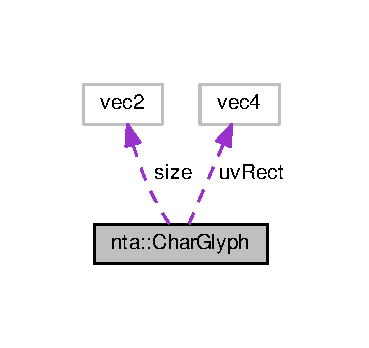
\includegraphics[width=177pt]{df/ddc/structnta_1_1CharGlyph__coll__graph}
\end{center}
\end{figure}
\begin{DoxyFields}{Class Members}
\mbox{\Hypertarget{namespacenta_aa2a40e6fe48ffadb4c7c95af7e82db91}\label{namespacenta_aa2a40e6fe48ffadb4c7c95af7e82db91}} 
vec2&
size&
the size of the rendered glyph \\
\hline

\mbox{\Hypertarget{namespacenta_a46d9ea9c38c8bf5e1c1679e938019f53}\label{namespacenta_a46d9ea9c38c8bf5e1c1679e938019f53}} 
vec4&
uvRect&
the rectangle containing this glyph in the texture \\
\hline

\end{DoxyFields}
\index{nta\+::\+G\+L\+Texture@{nta\+::\+G\+L\+Texture}}\label{structnta_1_1GLTexture}
\Hypertarget{namespacenta_structnta_1_1GLTexture}
\subsubsection{struct nta\+:\+:G\+L\+Texture}
represents a texture 

Definition at line 11 of file G\+L\+Texture.\+h.



Collaboration diagram for nta\+:\+:G\+L\+Texture\+:\nopagebreak
\begin{figure}[H]
\begin{center}
\leavevmode
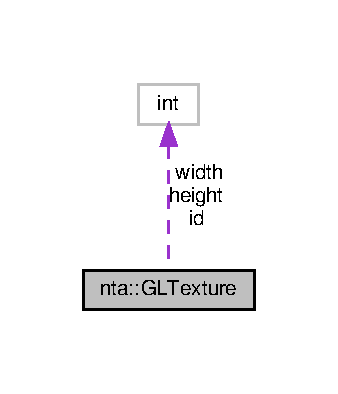
\includegraphics[width=162pt]{d3/d3e/structnta_1_1GLTexture__coll__graph}
\end{center}
\end{figure}
\begin{DoxyFields}{Class Members}
\mbox{\Hypertarget{namespacenta_a4ac2e45733ffb16238eb696d663e62a1}\label{namespacenta_a4ac2e45733ffb16238eb696d663e62a1}} 
GLint&
height&
\\
\hline

\mbox{\Hypertarget{namespacenta_aaf0d536088f4b1062d996679b217c0f9}\label{namespacenta_aaf0d536088f4b1062d996679b217c0f9}} 
GLuint&
id&
the id of the texture \\
\hline

\mbox{\Hypertarget{namespacenta_a8f4d13ab2b19b700f76334c46458ac48}\label{namespacenta_a8f4d13ab2b19b700f76334c46458ac48}} 
GLint&
width&
the width and height, respectively, of the texture \\
\hline

\end{DoxyFields}
\index{nta\+::\+Sprite\+Sheet.\+\_\+\+\_\+unnamed\+\_\+\+\_\+@{nta\+::\+Sprite\+Sheet.\+\_\+\+\_\+unnamed\+\_\+\+\_\+}}\label{unionnta_1_1SpriteSheet_8____unnamed____}
\Hypertarget{namespacenta_unionnta_1_1SpriteSheet_8____unnamed____}
\subsubsection{union nta\+:\+:Sprite\+Sheet.\+\_\+\+\_\+unnamed\+\_\+\+\_\+}
The dimensions of the sheat (rows x cols) 

Definition at line 38 of file Animation2\+D.\+h.

\begin{DoxyFields}{Class Members}
\mbox{\Hypertarget{namespacenta_a1378d7d8767899287b0407055215aa4e}\label{namespacenta_a1378d7d8767899287b0407055215aa4e}} 
\hyperlink{namespacenta_df/d10/structnta_1_1SpriteSheet_8____unnamed_____8____unnamed____}{\_\_unnamed\_\_}&
\_\_unnamed\_\_&
\\
\hline

\mbox{\Hypertarget{namespacenta_a5927205243f12cdc70612cba6dc874fa}\label{namespacenta_a5927205243f12cdc70612cba6dc874fa}} 
ivec2&
dims&
\\
\hline

\end{DoxyFields}
\index{nta\+::\+Sprite\+Sheet.\+\_\+\+\_\+unnamed\+\_\+\+\_\+.\+\_\+\+\_\+unnamed\+\_\+\+\_\+@{nta\+::\+Sprite\+Sheet.\+\_\+\+\_\+unnamed\+\_\+\+\_\+.\+\_\+\+\_\+unnamed\+\_\+\+\_\+}}\label{structnta_1_1SpriteSheet_8____unnamed_____8____unnamed____}
\Hypertarget{namespacenta_structnta_1_1SpriteSheet_8____unnamed_____8____unnamed____}
\subsubsection{struct nta\+:\+:Sprite\+Sheet.\+\_\+\+\_\+unnamed\+\_\+\+\_\+.\+\_\+\+\_\+unnamed\+\_\+\+\_\+}


Definition at line 40 of file Animation2\+D.\+h.

\begin{DoxyFields}{Class Members}
\mbox{\Hypertarget{namespacenta_a2ec7686cdf35752083c4cb22b93e362e}\label{namespacenta_a2ec7686cdf35752083c4cb22b93e362e}} 
int&
num\_cols&
\\
\hline

\mbox{\Hypertarget{namespacenta_ab428d91d44d86e0b79d1a3193951b762}\label{namespacenta_ab428d91d44d86e0b79d1a3193951b762}} 
int&
num\_rows&
\\
\hline

\end{DoxyFields}
\index{nta\+::\+Vertex\+Attrib@{nta\+::\+Vertex\+Attrib}}\label{structnta_1_1VertexAttrib}
\Hypertarget{namespacenta_structnta_1_1VertexAttrib}
\subsubsection{struct nta\+:\+:Vertex\+Attrib}
represents an attribute of a vertex (e.\+g. a call to gl\+Vertex\+Attrib\+Pointer) 

Definition at line 12 of file Vertex.\+h.



Collaboration diagram for nta\+:\+:Vertex\+Attrib\+:\nopagebreak
\begin{figure}[H]
\begin{center}
\leavevmode
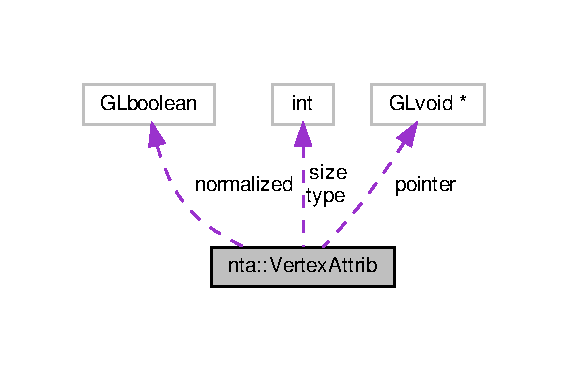
\includegraphics[width=273pt]{d6/d7d/structnta_1_1VertexAttrib__coll__graph}
\end{center}
\end{figure}
\begin{DoxyFields}{Class Members}
\mbox{\Hypertarget{namespacenta_afe78648a02032d5ba376207cf322320a}\label{namespacenta_afe78648a02032d5ba376207cf322320a}} 
GLboolean&
normalized&
\\
\hline

\mbox{\Hypertarget{namespacenta_a926cbe1d958dd6e72ad7f93e8791d9a4}\label{namespacenta_a926cbe1d958dd6e72ad7f93e8791d9a4}} 
GLvoid $\ast$&
pointer&
\\
\hline

\mbox{\Hypertarget{namespacenta_afd253a525c4d086bcc2afa66a2d0118e}\label{namespacenta_afd253a525c4d086bcc2afa66a2d0118e}} 
GLint&
size&
\\
\hline

\mbox{\Hypertarget{namespacenta_a625cbe8f28739965a9ec29b9a426465e}\label{namespacenta_a625cbe8f28739965a9ec29b9a426465e}} 
GLenum&
type&
\\
\hline

\end{DoxyFields}

\hypertarget{namespacenta_1_1utils}{}\section{nta\+:\+:utils Namespace Reference}
\label{namespacenta_1_1utils}\index{nta\+::utils@{nta\+::utils}}


Namespace for classes/functionality not necessarily specific to game/opengl development.  


\subsection*{Classes}
\begin{DoxyCompactItemize}
\item 
class \hyperlink{classnta_1_1utils_1_1IDFactory}{I\+D\+Factory}
\begin{DoxyCompactList}\small\item\em Class for generating unique (integral) I\+Ds. \end{DoxyCompactList}\item 
class \hyperlink{classnta_1_1utils_1_1Json}{Json}
\item 
class \hyperlink{classnta_1_1utils_1_1JsonNum}{Json\+Num}
\item 
struct \hyperlink{structnta_1_1utils_1_1LinkedNode}{Linked\+Node}
\begin{DoxyCompactList}\small\item\em A generic linked list. \end{DoxyCompactList}\item 
class \hyperlink{classnta_1_1utils_1_1Path}{Path}
\begin{DoxyCompactList}\small\item\em A (case-\/sensitive) \hyperlink{classnta_1_1utils_1_1Path}{Path} in a file system. \end{DoxyCompactList}\item 
class \hyperlink{classnta_1_1utils_1_1Semaphore}{Semaphore}
\item 
class \hyperlink{classnta_1_1utils_1_1ThreadPool}{Thread\+Pool}
\begin{DoxyCompactList}\small\item\em Collection of threads for running scheduled functions. \end{DoxyCompactList}\item 
struct \hyperlink{structnta_1_1utils_1_1TypeInfo}{Type\+Info}
\begin{DoxyCompactList}\small\item\em Struct for storing basic information about a type used by \hyperlink{classnta_1_1utils_1_1TypeMap}{Type\+Map}. \end{DoxyCompactList}\item 
class \hyperlink{classnta_1_1utils_1_1TypeMap}{Type\+Map}
\end{DoxyCompactItemize}
\subsection*{Typedefs}
\begin{DoxyCompactItemize}
\item 
\mbox{\Hypertarget{namespacenta_1_1utils_aacec41f909698427351bd2d4e6bfb0ff}\label{namespacenta_1_1utils_aacec41f909698427351bd2d4e6bfb0ff}} 
typedef std\+::map$<$ std\+::string, \hyperlink{classnta_1_1utils_1_1Json}{Json} $>$ {\bfseries Json\+Object}
\item 
\mbox{\Hypertarget{namespacenta_1_1utils_a016ff68f749b52514dae354976f110ea}\label{namespacenta_1_1utils_a016ff68f749b52514dae354976f110ea}} 
typedef std\+::vector$<$ \hyperlink{classnta_1_1utils_1_1Json}{Json} $>$ {\bfseries Json\+Array}
\end{DoxyCompactItemize}
\subsection*{Enumerations}
\begin{DoxyCompactItemize}
\item 
\mbox{\Hypertarget{namespacenta_1_1utils_a83ee7c4cfccd9fa43564f5fe1c0c77d3}\label{namespacenta_1_1utils_a83ee7c4cfccd9fa43564f5fe1c0c77d3}} 
enum \hyperlink{namespacenta_1_1utils_a83ee7c4cfccd9fa43564f5fe1c0c77d3}{Json\+Num\+Type} \{ {\bfseries P\+O\+S\+\_\+\+I\+NT}, 
{\bfseries N\+E\+G\+\_\+\+I\+NT}, 
{\bfseries F\+L\+O\+AT}
 \}\begin{DoxyCompactList}\small\item\em The various types a Json number can take. \end{DoxyCompactList}
\item 
\mbox{\Hypertarget{namespacenta_1_1utils_ac9921c0a3baf86d9facdc4927c66def3}\label{namespacenta_1_1utils_ac9921c0a3baf86d9facdc4927c66def3}} 
enum \hyperlink{namespacenta_1_1utils_ac9921c0a3baf86d9facdc4927c66def3}{Json\+Value\+Type} \{ \newline
{\bfseries S\+T\+R\+I\+NG} = 0, 
{\bfseries N\+U\+M\+B\+ER} = 1, 
{\bfseries O\+B\+J\+E\+CT} = 2, 
{\bfseries A\+R\+R\+AY} = 3, 
\newline
{\bfseries B\+O\+O\+L\+E\+AN} = 4, 
{\bfseries N\+O\+NE} = 5
 \}\begin{DoxyCompactList}\small\item\em The various Json types. \end{DoxyCompactList}
\end{DoxyCompactItemize}
\subsection*{Functions}
\begin{DoxyCompactItemize}
\item 
\mbox{\Hypertarget{namespacenta_1_1utils_aafbc0cf6600011397dc89456e14a706f}\label{namespacenta_1_1utils_aafbc0cf6600011397dc89456e14a706f}} 
std\+::ostream \& {\bfseries operator$<$$<$} (std\+::ostream \&out, const \hyperlink{classnta_1_1utils_1_1Path}{Path} \&path)
\item 
\mbox{\Hypertarget{namespacenta_1_1utils_a9ad5fe63f14dd42c0db25d71e101e85c}\label{namespacenta_1_1utils_a9ad5fe63f14dd42c0db25d71e101e85c}} 
bool \hyperlink{namespacenta_1_1utils_a9ad5fe63f14dd42c0db25d71e101e85c}{starts\+\_\+with} (crstring str, crstring prefix)
\begin{DoxyCompactList}\small\item\em Checks if str starts with prefix. \end{DoxyCompactList}\item 
\mbox{\Hypertarget{namespacenta_1_1utils_aa31e7ef45edfc4fdb60b6459e86b519c}\label{namespacenta_1_1utils_aa31e7ef45edfc4fdb60b6459e86b519c}} 
bool \hyperlink{namespacenta_1_1utils_aa31e7ef45edfc4fdb60b6459e86b519c}{ends\+\_\+with} (crstring str, crstring suffix)
\begin{DoxyCompactList}\small\item\em Checks if str ends with suffix. \end{DoxyCompactList}\item 
\mbox{\Hypertarget{namespacenta_1_1utils_acad0765e34bce437d37871dcf88a9099}\label{namespacenta_1_1utils_acad0765e34bce437d37871dcf88a9099}} 
std\+::string \hyperlink{namespacenta_1_1utils_acad0765e34bce437d37871dcf88a9099}{replace\+\_\+all} (crstring str, crstring o, crstring n)
\begin{DoxyCompactList}\small\item\em Replaces all occurences of o in str with n. \end{DoxyCompactList}\item 
\mbox{\Hypertarget{namespacenta_1_1utils_ac35b6baec75cd7b9d9ab7532cc2f9320}\label{namespacenta_1_1utils_ac35b6baec75cd7b9d9ab7532cc2f9320}} 
std\+::string \hyperlink{namespacenta_1_1utils_ac35b6baec75cd7b9d9ab7532cc2f9320}{replace\+\_\+all} (crstring str, const std\+::vector$<$ std\+::vector$<$ std\+::string $>$$>$ \&os, const std\+::vector$<$ std\+::string $>$ \&ns)
\begin{DoxyCompactList}\small\item\em Replaces all occurences of any string in the ith element of os with the ith element of ns. \end{DoxyCompactList}\item 
\mbox{\Hypertarget{namespacenta_1_1utils_af4c37b245aa436ad6022581a347feb01}\label{namespacenta_1_1utils_af4c37b245aa436ad6022581a347feb01}} 
std\+::string \hyperlink{namespacenta_1_1utils_af4c37b245aa436ad6022581a347feb01}{trim} (crstring str, crstring back\+\_\+trash=\char`\"{} \textbackslash{}\textbackslash{}\textbackslash{}\char`\"{}, crstring front\+\_\+trash=\char`\"{} \textbackslash{}\textbackslash{}\textbackslash{}\char`\"{})
\begin{DoxyCompactList}\small\item\em Removes leading and trailing whitespace. \end{DoxyCompactList}\item 
\mbox{\Hypertarget{namespacenta_1_1utils_ae2b6ac39c9975a5ca13c417395fae759}\label{namespacenta_1_1utils_ae2b6ac39c9975a5ca13c417395fae759}} 
std\+::vector$<$ std\+::string $>$ \hyperlink{namespacenta_1_1utils_ae2b6ac39c9975a5ca13c417395fae759}{split} (crstring str, char delim)
\begin{DoxyCompactList}\small\item\em Splits a string into substrings separated by delim. \end{DoxyCompactList}\item 
\mbox{\Hypertarget{namespacenta_1_1utils_a4171db688c28bc11eb63d3ad0e8bf136}\label{namespacenta_1_1utils_a4171db688c28bc11eb63d3ad0e8bf136}} 
glm\+::vec2 \hyperlink{namespacenta_1_1utils_a4171db688c28bc11eb63d3ad0e8bf136}{rotate} (crvec2 pt, float angle)
\begin{DoxyCompactList}\small\item\em Rotates a point (about the origin) by the given angle. \end{DoxyCompactList}\item 
\mbox{\Hypertarget{namespacenta_1_1utils_aab201e3eaa7a7d050ca81ca029ec2347}\label{namespacenta_1_1utils_aab201e3eaa7a7d050ca81ca029ec2347}} 
{\footnotesize template$<$class T $>$ }\\std\+::string \hyperlink{namespacenta_1_1utils_aab201e3eaa7a7d050ca81ca029ec2347}{to\+\_\+string} (const T \&input, std\+::size\+\_\+t precision=0)
\begin{DoxyCompactList}\small\item\em converts input to a std\+::string \end{DoxyCompactList}\item 
\mbox{\Hypertarget{namespacenta_1_1utils_aaa025ad45973ff6dc3a33800ccea72f0}\label{namespacenta_1_1utils_aaa025ad45973ff6dc3a33800ccea72f0}} 
{\footnotesize template$<$class T $>$ }\\bool \hyperlink{namespacenta_1_1utils_aaa025ad45973ff6dc3a33800ccea72f0}{in\+\_\+range} (T val, T min, T max)
\begin{DoxyCompactList}\small\item\em returns whether or not min $<$= val $<$= max \end{DoxyCompactList}\end{DoxyCompactItemize}


\subsection{Detailed Description}
Namespace for classes/functionality not necessarily specific to game/opengl development. 
\chapter{Class Documentation}
\hypertarget{classnta_1_1Animation2D}{}\section{nta\+:\+:Animation2D Class Reference}
\label{classnta_1_1Animation2D}\index{nta\+::\+Animation2D@{nta\+::\+Animation2D}}


A 2D Animation made from a single \hyperlink{structnta_1_1SpriteSheet}{Sprite\+Sheet}.  




{\ttfamily \#include $<$Animation2\+D.\+h$>$}

\subsection*{Public Member Functions}
\begin{DoxyCompactItemize}
\item 
\mbox{\Hypertarget{classnta_1_1Animation2D_a792bd9b44d471dc526e89dc9b2b4b7e0}\label{classnta_1_1Animation2D_a792bd9b44d471dc526e89dc9b2b4b7e0}} 
{\bfseries Animation2D} (const \hyperlink{structnta_1_1SpriteSheet}{Sprite\+Sheet} \&sheet, std\+::size\+\_\+t start=0, std\+::size\+\_\+t length=1, float speed=1)
\item 
\mbox{\Hypertarget{classnta_1_1Animation2D_a914bde6d79c34f2da580c9de07460e51}\label{classnta_1_1Animation2D_a914bde6d79c34f2da580c9de07460e51}} 
{\bfseries Animation2D} (crstring file\+\_\+path, crivec2 dims, std\+::size\+\_\+t start=0, std\+::size\+\_\+t length=1, float speed=1)
\item 
\mbox{\Hypertarget{classnta_1_1Animation2D_af7e829c4535ff57a41cfecbb9313ef7b}\label{classnta_1_1Animation2D_af7e829c4535ff57a41cfecbb9313ef7b}} 
{\bfseries Animation2D} (crstring file\+\_\+path, int num\+\_\+cols, std\+::size\+\_\+t start=0, std\+::size\+\_\+t length=1, float speed=1)
\item 
\mbox{\Hypertarget{classnta_1_1Animation2D_af7373ff1020b685bd583ae63ba24de55}\label{classnta_1_1Animation2D_af7373ff1020b685bd583ae63ba24de55}} 
glm\+::vec4 {\bfseries get\+\_\+uv} () const
\item 
\mbox{\Hypertarget{classnta_1_1Animation2D_aa46a6c17839ad28c1f6b4c04537b237a}\label{classnta_1_1Animation2D_aa46a6c17839ad28c1f6b4c04537b237a}} 
glm\+::vec4 {\bfseries get\+\_\+flipped\+\_\+uv} () const
\item 
\mbox{\Hypertarget{classnta_1_1Animation2D_a1192a17d29aa798e21eed8a93bd0387a}\label{classnta_1_1Animation2D_a1192a17d29aa798e21eed8a93bd0387a}} 
glm\+::vec2 {\bfseries get\+\_\+frame\+\_\+dims} () const
\item 
\mbox{\Hypertarget{classnta_1_1Animation2D_ac446522438b03f14a532907ba5c3d5af}\label{classnta_1_1Animation2D_ac446522438b03f14a532907ba5c3d5af}} 
std\+::size\+\_\+t {\bfseries get\+\_\+index} () const
\item 
\mbox{\Hypertarget{classnta_1_1Animation2D_a27647ebb0767d114b3330d784be76659}\label{classnta_1_1Animation2D_a27647ebb0767d114b3330d784be76659}} 
std\+::size\+\_\+t {\bfseries get\+\_\+start} () const
\item 
\mbox{\Hypertarget{classnta_1_1Animation2D_a879e528e64c38508ecab2dfff935d5d9}\label{classnta_1_1Animation2D_a879e528e64c38508ecab2dfff935d5d9}} 
std\+::size\+\_\+t {\bfseries get\+\_\+length} () const
\item 
\mbox{\Hypertarget{classnta_1_1Animation2D_ac9848d72d81b4391bffc40473bb6556e}\label{classnta_1_1Animation2D_ac9848d72d81b4391bffc40473bb6556e}} 
float {\bfseries get\+\_\+speed} () const
\item 
\mbox{\Hypertarget{classnta_1_1Animation2D_a0ad6c0188e2b36f42caf1817537ec483}\label{classnta_1_1Animation2D_a0ad6c0188e2b36f42caf1817537ec483}} 
G\+Luint {\bfseries get\+\_\+tex\+\_\+id} () const
\item 
\mbox{\Hypertarget{classnta_1_1Animation2D_aa0aae6f2c69f9edb1e5f0dc35a440e48}\label{classnta_1_1Animation2D_aa0aae6f2c69f9edb1e5f0dc35a440e48}} 
float {\bfseries get\+\_\+time} () const
\item 
\mbox{\Hypertarget{classnta_1_1Animation2D_aa5de467f16ecc3851bcfbf1da68a6103}\label{classnta_1_1Animation2D_aa5de467f16ecc3851bcfbf1da68a6103}} 
void {\bfseries switch\+\_\+animation} (std\+::size\+\_\+t start, std\+::size\+\_\+t length, float speed=1)
\item 
\mbox{\Hypertarget{classnta_1_1Animation2D_ab22616e5abdf38980404a711503f1b99}\label{classnta_1_1Animation2D_ab22616e5abdf38980404a711503f1b99}} 
void {\bfseries set\+\_\+speed} (float speed)
\item 
\mbox{\Hypertarget{classnta_1_1Animation2D_a3bc6f94232a04f3302ab5670ab46be44}\label{classnta_1_1Animation2D_a3bc6f94232a04f3302ab5670ab46be44}} 
void {\bfseries step} (float dt)
\end{DoxyCompactItemize}
\subsection*{Private Attributes}
\begin{DoxyCompactItemize}
\item 
\mbox{\Hypertarget{classnta_1_1Animation2D_a7299c55bbae2e3a8eed7bbfde8362523}\label{classnta_1_1Animation2D_a7299c55bbae2e3a8eed7bbfde8362523}} 
\hyperlink{structnta_1_1SpriteSheet}{Sprite\+Sheet} \hyperlink{classnta_1_1Animation2D_a7299c55bbae2e3a8eed7bbfde8362523}{m\+\_\+sheet}
\begin{DoxyCompactList}\small\item\em The sheet holding the sprites used by the animation. \end{DoxyCompactList}\item 
\mbox{\Hypertarget{classnta_1_1Animation2D_a24497412429334fe270a1b0ba6526203}\label{classnta_1_1Animation2D_a24497412429334fe270a1b0ba6526203}} 
float \hyperlink{classnta_1_1Animation2D_a24497412429334fe270a1b0ba6526203}{m\+\_\+time}
\begin{DoxyCompactList}\small\item\em how far along in the animation we are \end{DoxyCompactList}\item 
\mbox{\Hypertarget{classnta_1_1Animation2D_ae2df81906b0e98c7df18ed19950695e7}\label{classnta_1_1Animation2D_ae2df81906b0e98c7df18ed19950695e7}} 
float \hyperlink{classnta_1_1Animation2D_ae2df81906b0e98c7df18ed19950695e7}{m\+\_\+speed}
\begin{DoxyCompactList}\small\item\em how quickly the animation advances when step is called \end{DoxyCompactList}\item 
\mbox{\Hypertarget{classnta_1_1Animation2D_a61cdaf3599067dc1e2fe3b926b29b838}\label{classnta_1_1Animation2D_a61cdaf3599067dc1e2fe3b926b29b838}} 
std\+::size\+\_\+t \hyperlink{classnta_1_1Animation2D_a61cdaf3599067dc1e2fe3b926b29b838}{m\+\_\+start\+\_\+index}
\begin{DoxyCompactList}\small\item\em A single animation spans m\+\_\+length continuous sprite indices begging with m\+\_\+start\+\_\+index. \end{DoxyCompactList}\item 
\mbox{\Hypertarget{classnta_1_1Animation2D_a7ad254603c0e4c081895989643f6aa9e}\label{classnta_1_1Animation2D_a7ad254603c0e4c081895989643f6aa9e}} 
std\+::size\+\_\+t {\bfseries m\+\_\+length}
\end{DoxyCompactItemize}


\subsection{Detailed Description}
A 2D Animation made from a single \hyperlink{structnta_1_1SpriteSheet}{Sprite\+Sheet}. 

Definition at line 51 of file Animation2\+D.\+h.



Collaboration diagram for nta\+:\+:Animation2D\+:\nopagebreak
\begin{figure}[H]
\begin{center}
\leavevmode
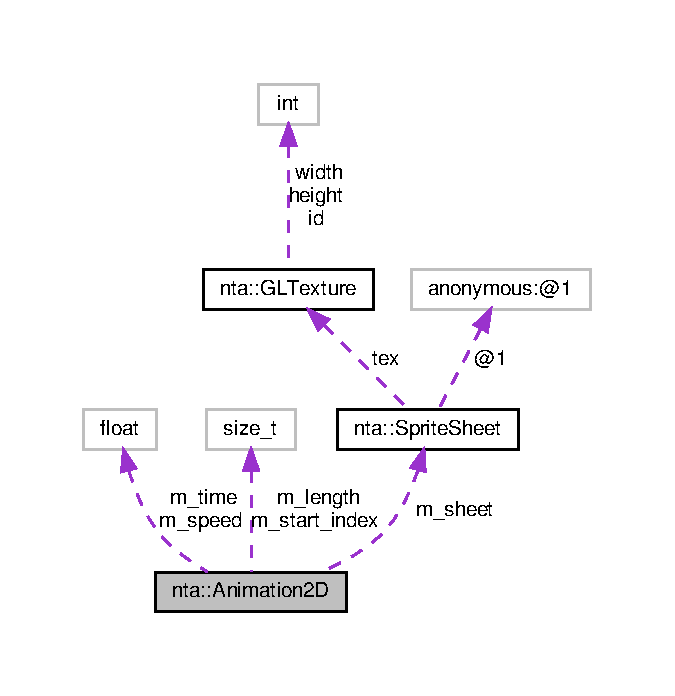
\includegraphics[width=324pt]{db/d21/classnta_1_1Animation2D__coll__graph}
\end{center}
\end{figure}


The documentation for this class was generated from the following files\+:\begin{DoxyCompactItemize}
\item 
include/nta/Animation2\+D.\+h\item 
src/Animation2\+D.\+cpp\end{DoxyCompactItemize}

\hypertarget{classnta_1_1AudioManager}{}\section{nta\+:\+:Audio\+Manager Class Reference}
\label{classnta_1_1AudioManager}\index{nta\+::\+Audio\+Manager@{nta\+::\+Audio\+Manager}}
\subsection*{Static Public Member Functions}
\begin{DoxyCompactItemize}
\item 
\mbox{\Hypertarget{classnta_1_1AudioManager_a4da570a6cee16bd6450031f7910057fd}\label{classnta_1_1AudioManager_a4da570a6cee16bd6450031f7910057fd}} 
static void \hyperlink{classnta_1_1AudioManager_a4da570a6cee16bd6450031f7910057fd}{init} ()
\begin{DoxyCompactList}\small\item\em initializes S\+D\+L\+\_\+\+Mixer \end{DoxyCompactList}\item 
\mbox{\Hypertarget{classnta_1_1AudioManager_aa337e5cc1825c6e2b971e1fc173b17ce}\label{classnta_1_1AudioManager_aa337e5cc1825c6e2b971e1fc173b17ce}} 
static void \hyperlink{classnta_1_1AudioManager_aa337e5cc1825c6e2b971e1fc173b17ce}{destroy} ()
\begin{DoxyCompactList}\small\item\em frees all music \end{DoxyCompactList}\item 
\mbox{\Hypertarget{classnta_1_1AudioManager_a131e8ec62c63fd9a07a77d833b02b598}\label{classnta_1_1AudioManager_a131e8ec62c63fd9a07a77d833b02b598}} 
static \hyperlink{classnta_1_1SoundEffect}{Sound\+Effect} $\ast$ \hyperlink{classnta_1_1AudioManager_a131e8ec62c63fd9a07a77d833b02b598}{get\+Sound\+Effect} (crstring effect\+Path)
\begin{DoxyCompactList}\small\item\em returns sound \end{DoxyCompactList}\item 
\mbox{\Hypertarget{classnta_1_1AudioManager_adb0a0f0efb072f57430835c849caaa39}\label{classnta_1_1AudioManager_adb0a0f0efb072f57430835c849caaa39}} 
static \hyperlink{classnta_1_1Music}{Music} $\ast$ {\bfseries get\+Music} (crstring music\+Path)
\end{DoxyCompactItemize}
\subsection*{Static Private Attributes}
\begin{DoxyCompactItemize}
\item 
\mbox{\Hypertarget{classnta_1_1AudioManager_a745f3ef1216f7e6bf848a9eb4054c5b4}\label{classnta_1_1AudioManager_a745f3ef1216f7e6bf848a9eb4054c5b4}} 
static std\+::map$<$ std\+::string, \hyperlink{classnta_1_1SoundEffect}{Sound\+Effect} $\ast$ $>$ \hyperlink{classnta_1_1AudioManager_a745f3ef1216f7e6bf848a9eb4054c5b4}{m\+\_\+effect\+Map}
\begin{DoxyCompactList}\small\item\em maps for associating sounds with their files \end{DoxyCompactList}\item 
\mbox{\Hypertarget{classnta_1_1AudioManager_ae301717a98c3a7bb0ca0b588c270b122}\label{classnta_1_1AudioManager_ae301717a98c3a7bb0ca0b588c270b122}} 
static std\+::map$<$ std\+::string, \hyperlink{classnta_1_1Music}{Music} $\ast$ $>$ {\bfseries m\+\_\+music\+Map}
\end{DoxyCompactItemize}


\subsection{Detailed Description}


Definition at line 65 of file Audio\+Manager.\+h.



Collaboration diagram for nta\+:\+:Audio\+Manager\+:\nopagebreak
\begin{figure}[H]
\begin{center}
\leavevmode
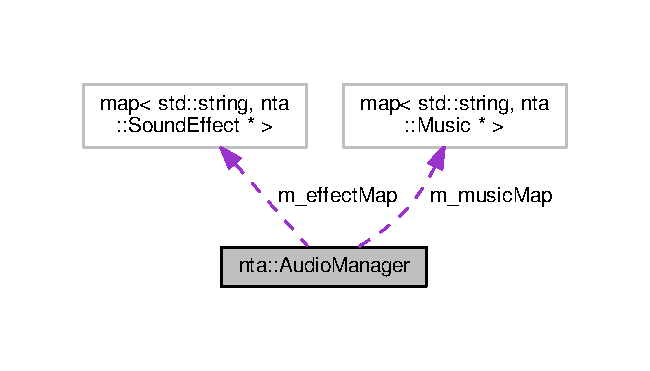
\includegraphics[width=312pt]{d9/d95/classnta_1_1AudioManager__coll__graph}
\end{center}
\end{figure}


The documentation for this class was generated from the following files\+:\begin{DoxyCompactItemize}
\item 
include/nta/Audio\+Manager.\+h\item 
src/Audio\+Manager.\+cpp\end{DoxyCompactItemize}

\hypertarget{classnta_1_1CallbackManager}{}\section{nta\+:\+:Callback\+Manager Class Reference}
\label{classnta_1_1CallbackManager}\index{nta\+::\+Callback\+Manager@{nta\+::\+Callback\+Manager}}


{\ttfamily \#include $<$Callback\+Manager.\+h$>$}

\subsection*{Classes}
\begin{DoxyCompactItemize}
\item 
struct \hyperlink{classnta_1_1CallbackManager_d3/dc5/structnta_1_1CallbackManager_1_1event}{event}
\begin{DoxyCompactList}\small\item\em A function to run at a certain time with some regularity.  \hyperlink{classnta_1_1CallbackManager_d3/dc5/structnta_1_1CallbackManager_1_1event}{More...}\end{DoxyCompactList}\end{DoxyCompactItemize}
\subsection*{Static Public Member Functions}
\begin{DoxyCompactItemize}
\item 
static uint64\+\_\+t \hyperlink{classnta_1_1CallbackManager_a1fd6132e79e49dbcb787bc8a8507a931}{set\+Interval} (const Thunk \&thunk, uint64\+\_\+t when, uint64\+\_\+t period)
\item 
\mbox{\Hypertarget{classnta_1_1CallbackManager_ac51c18a014641ffe9dbfe8ead0f6bae0}\label{classnta_1_1CallbackManager_ac51c18a014641ffe9dbfe8ead0f6bae0}} 
static uint64\+\_\+t \hyperlink{classnta_1_1CallbackManager_ac51c18a014641ffe9dbfe8ead0f6bae0}{set\+Timeout} (const Thunk \&thunk, uint64\+\_\+t when)
\begin{DoxyCompactList}\small\item\em Schedules a function to be called once after when frames and then repeatedly after. \end{DoxyCompactList}\item 
\mbox{\Hypertarget{classnta_1_1CallbackManager_af184e9fbc5353c8e019cf61c51c03448}\label{classnta_1_1CallbackManager_af184e9fbc5353c8e019cf61c51c03448}} 
static bool \hyperlink{classnta_1_1CallbackManager_af184e9fbc5353c8e019cf61c51c03448}{delay} (uint64\+\_\+t id, uint64\+\_\+t when, bool absolute=true)
\begin{DoxyCompactList}\small\item\em Changes when an event is next scheduled to run. \end{DoxyCompactList}\item 
\mbox{\Hypertarget{classnta_1_1CallbackManager_a2c8114a6c1e8de9c59b6484f47dde1a3}\label{classnta_1_1CallbackManager_a2c8114a6c1e8de9c59b6484f47dde1a3}} 
static void \hyperlink{classnta_1_1CallbackManager_a2c8114a6c1e8de9c59b6484f47dde1a3}{init} ()
\begin{DoxyCompactList}\small\item\em Initializes the \hyperlink{classnta_1_1CallbackManager}{Callback\+Manager}. \end{DoxyCompactList}\item 
\mbox{\Hypertarget{classnta_1_1CallbackManager_a4af0feb66d42bd32d5bde2e4a52519a9}\label{classnta_1_1CallbackManager_a4af0feb66d42bd32d5bde2e4a52519a9}} 
static void \hyperlink{classnta_1_1CallbackManager_a4af0feb66d42bd32d5bde2e4a52519a9}{clear} (uint64\+\_\+t id)
\begin{DoxyCompactList}\small\item\em Removes the event with the given id. \end{DoxyCompactList}\item 
\mbox{\Hypertarget{classnta_1_1CallbackManager_ae055387e26996a024065a5b59c833e78}\label{classnta_1_1CallbackManager_ae055387e26996a024065a5b59c833e78}} 
static void \hyperlink{classnta_1_1CallbackManager_ae055387e26996a024065a5b59c833e78}{increment\+\_\+frame} ()
\begin{DoxyCompactList}\small\item\em Informs \hyperlink{classnta_1_1CallbackManager}{Callback\+Manager} that a frame has passed. \end{DoxyCompactList}\item 
\mbox{\Hypertarget{classnta_1_1CallbackManager_a70be77ca2505257376250c660a3082d6}\label{classnta_1_1CallbackManager_a70be77ca2505257376250c660a3082d6}} 
static void \hyperlink{classnta_1_1CallbackManager_a70be77ca2505257376250c660a3082d6}{destroy} ()
\begin{DoxyCompactList}\small\item\em Destroys the \hyperlink{classnta_1_1CallbackManager}{Callback\+Manager}. \end{DoxyCompactList}\end{DoxyCompactItemize}
\subsection*{Static Private Member Functions}
\begin{DoxyCompactItemize}
\item 
static void \hyperlink{classnta_1_1CallbackManager_a7912dc908d7a7a44267ddd8fa6fb8686}{dispatch} ()
\item 
\mbox{\Hypertarget{classnta_1_1CallbackManager_a897df241a317572ff96bb89e28aadc14}\label{classnta_1_1CallbackManager_a897df241a317572ff96bb89e28aadc14}} 
static void \hyperlink{classnta_1_1CallbackManager_a897df241a317572ff96bb89e28aadc14}{dequeue} (uint64\+\_\+t id)
\begin{DoxyCompactList}\small\item\em Removes event from m\+\_\+queue but not m\+\_\+active (assumes id is valid) \end{DoxyCompactList}\end{DoxyCompactItemize}
\subsection*{Static Private Attributes}
\begin{DoxyCompactItemize}
\item 
\mbox{\Hypertarget{classnta_1_1CallbackManager_a03df001cff1afcc19ed4bb35cd51b5d0}\label{classnta_1_1CallbackManager_a03df001cff1afcc19ed4bb35cd51b5d0}} 
static std\+::map$<$ uint64\+\_\+t, \hyperlink{classnta_1_1CallbackManager_d3/dc5/structnta_1_1CallbackManager_1_1event}{event} $>$ \hyperlink{classnta_1_1CallbackManager_a03df001cff1afcc19ed4bb35cd51b5d0}{m\+\_\+active}
\begin{DoxyCompactList}\small\item\em The events waiting to happen (key is \hyperlink{classnta_1_1CallbackManager_a743978e02001b9ceff1145c41214d2e5}{event.\+id}) \end{DoxyCompactList}\item 
\mbox{\Hypertarget{classnta_1_1CallbackManager_af348c39ad7b27a0f8c92e4b90bf944a7}\label{classnta_1_1CallbackManager_af348c39ad7b27a0f8c92e4b90bf944a7}} 
static std\+::map$<$ uint64\+\_\+t, std\+::vector$<$ \hyperlink{classnta_1_1CallbackManager_d3/dc5/structnta_1_1CallbackManager_1_1event}{event} $\ast$ $>$ $>$ \hyperlink{classnta_1_1CallbackManager_af348c39ad7b27a0f8c92e4b90bf944a7}{m\+\_\+queue}
\begin{DoxyCompactList}\small\item\em \char`\"{}\+Priority queue\char`\"{} of events ordered by when they should occur \end{DoxyCompactList}\item 
\mbox{\Hypertarget{classnta_1_1CallbackManager_a4bdfb67cfd791112b1e83159862eefa0}\label{classnta_1_1CallbackManager_a4bdfb67cfd791112b1e83159862eefa0}} 
static \hyperlink{classnta_1_1utils_1_1ThreadPool}{utils\+::\+Thread\+Pool} \hyperlink{classnta_1_1CallbackManager_a4bdfb67cfd791112b1e83159862eefa0}{m\+\_\+pool}
\begin{DoxyCompactList}\small\item\em Thread\+Pool used for scheduling events to happen. \end{DoxyCompactList}\item 
\mbox{\Hypertarget{classnta_1_1CallbackManager_abc47b7e18fc1576edb799be131baf116}\label{classnta_1_1CallbackManager_abc47b7e18fc1576edb799be131baf116}} 
static std\+::thread \hyperlink{classnta_1_1CallbackManager_abc47b7e18fc1576edb799be131baf116}{m\+\_\+dispatcher}
\begin{DoxyCompactList}\small\item\em Thread used to dispatch events. \end{DoxyCompactList}\item 
\mbox{\Hypertarget{classnta_1_1CallbackManager_a714aa329a54538ec5bda528fa3a3ab7f}\label{classnta_1_1CallbackManager_a714aa329a54538ec5bda528fa3a3ab7f}} 
static std\+::atomic$<$ uint64\+\_\+t $>$ \hyperlink{classnta_1_1CallbackManager_a714aa329a54538ec5bda528fa3a3ab7f}{m\+\_\+next}
\begin{DoxyCompactList}\small\item\em id given to the next created event \end{DoxyCompactList}\item 
\mbox{\Hypertarget{classnta_1_1CallbackManager_a56903bee3075ab191f598e36438d6b50}\label{classnta_1_1CallbackManager_a56903bee3075ab191f598e36438d6b50}} 
static std\+::mutex {\bfseries m\+\_\+mutex}
\item 
\mbox{\Hypertarget{classnta_1_1CallbackManager_afa5d7642112c791dcfef35d78aff4d09}\label{classnta_1_1CallbackManager_afa5d7642112c791dcfef35d78aff4d09}} 
static std\+::condition\+\_\+variable\+\_\+any {\bfseries m\+\_\+cv}
\item 
\mbox{\Hypertarget{classnta_1_1CallbackManager_a20cd08f864fd62edbd68f5f309be5c30}\label{classnta_1_1CallbackManager_a20cd08f864fd62edbd68f5f309be5c30}} 
static bool \hyperlink{classnta_1_1CallbackManager_a20cd08f864fd62edbd68f5f309be5c30}{m\+\_\+working}
\begin{DoxyCompactList}\small\item\em Global flag saying whether or not the \hyperlink{classnta_1_1CallbackManager}{Callback\+Manager} has been destroyed. \end{DoxyCompactList}\item 
\mbox{\Hypertarget{classnta_1_1CallbackManager_a69bbc2e4ac29aca06d09b2466b6769c2}\label{classnta_1_1CallbackManager_a69bbc2e4ac29aca06d09b2466b6769c2}} 
static uint64\+\_\+t \hyperlink{classnta_1_1CallbackManager_a69bbc2e4ac29aca06d09b2466b6769c2}{m\+\_\+curr\+\_\+frame}
\begin{DoxyCompactList}\small\item\em The current frame. \end{DoxyCompactList}\end{DoxyCompactItemize}


\subsection{Detailed Description}
Allows scheduling of functions to be called at a later point in time \begin{DoxyRefDesc}{Todo}
\item[\hyperlink{todo__todo000001}{Todo}]Add ability to base timing off of actual time instead of frames 

Debug all this code. I was not at my best when I originally wrote it 

make non-\/static (ideally, one \hyperlink{classnta_1_1CallbackManager}{Callback\+Manager} per \hyperlink{classnta_1_1ScreenManager}{Screen\+Manager}) \end{DoxyRefDesc}


Definition at line 13 of file Callback\+Manager.\+h.



Collaboration diagram for nta\+:\+:Callback\+Manager\+:\nopagebreak
\begin{figure}[H]
\begin{center}
\leavevmode
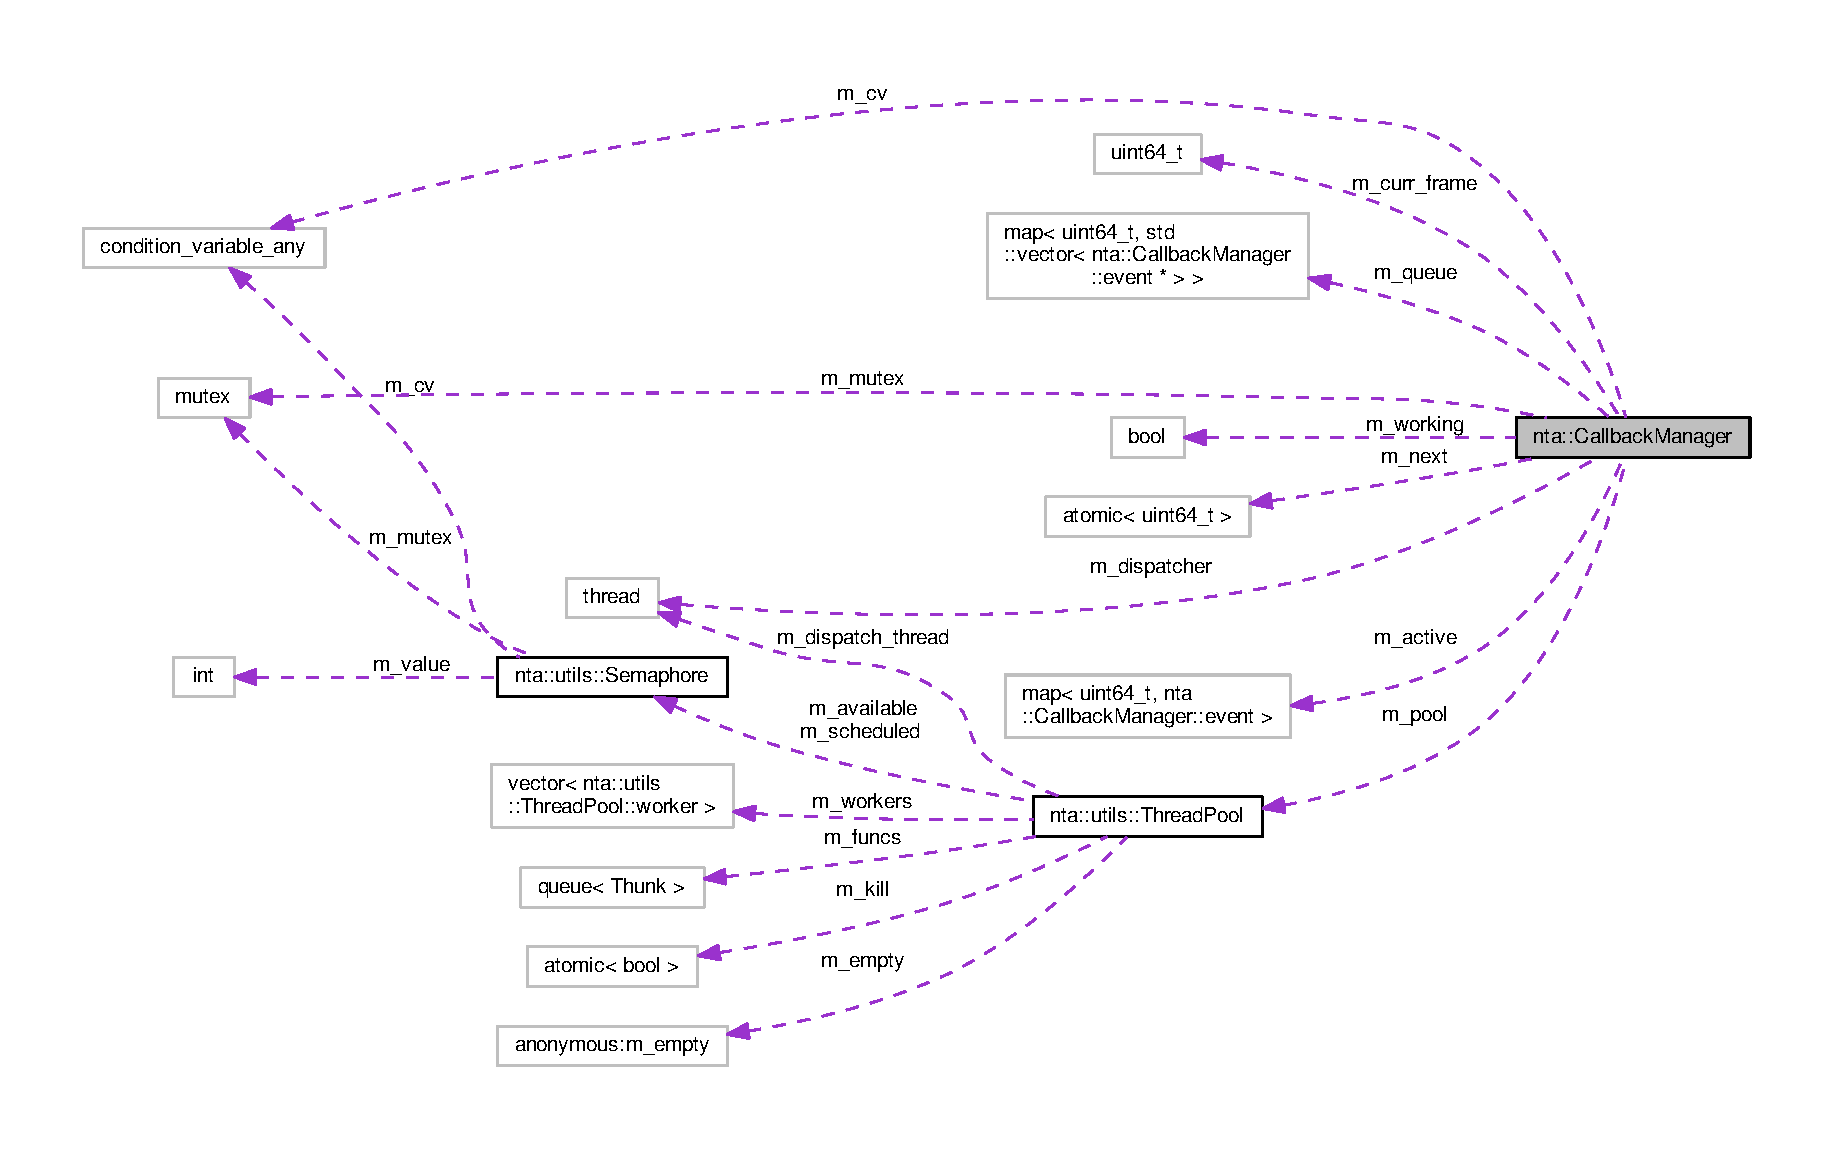
\includegraphics[width=350pt]{dc/df2/classnta_1_1CallbackManager__coll__graph}
\end{center}
\end{figure}


\subsection{Class Documentation}
\index{nta\+::\+Callback\+Manager\+::event@{nta\+::\+Callback\+Manager\+::event}}\label{structnta_1_1CallbackManager_1_1event}
\Hypertarget{classnta_1_1CallbackManager_structnta_1_1CallbackManager_1_1event}
\subsubsection{struct nta\+:\+:Callback\+Manager\+:\+:event}
A function to run at a certain time with some regularity. 

Definition at line 16 of file Callback\+Manager.\+h.



Collaboration diagram for nta\+:\+:Callback\+Manager\+:\+:event\+:\nopagebreak
\begin{figure}[H]
\begin{center}
\leavevmode
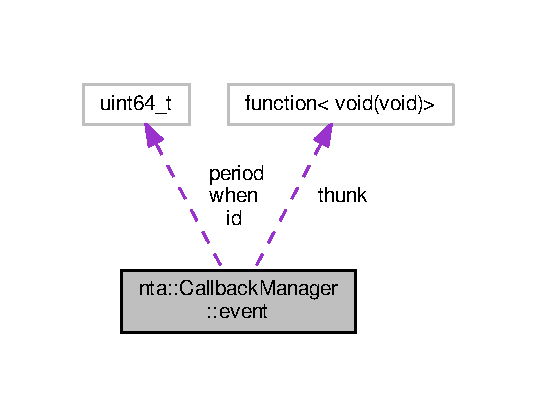
\includegraphics[width=258pt]{da/d01/structnta_1_1CallbackManager_1_1event__coll__graph}
\end{center}
\end{figure}
\begin{DoxyFields}{Class Members}
\mbox{\Hypertarget{classnta_1_1CallbackManager_a743978e02001b9ceff1145c41214d2e5}\label{classnta_1_1CallbackManager_a743978e02001b9ceff1145c41214d2e5}} 
uint64\_t&
id&
id of event \\
\hline

\mbox{\Hypertarget{classnta_1_1CallbackManager_a15dd99ac7d4588c5ac5518c063431ef5}\label{classnta_1_1CallbackManager_a15dd99ac7d4588c5ac5518c063431ef5}} 
uint64\_t&
period&
How many frames between consecutive runs. \\
\hline

\mbox{\Hypertarget{classnta_1_1CallbackManager_ad92bce3b5cee6411a2b2c08b4c13b767}\label{classnta_1_1CallbackManager_ad92bce3b5cee6411a2b2c08b4c13b767}} 
Thunk&
thunk&
Function to execute. \\
\hline

\mbox{\Hypertarget{classnta_1_1CallbackManager_ab20a0382304629ebdc2643a834c9dcff}\label{classnta_1_1CallbackManager_ab20a0382304629ebdc2643a834c9dcff}} 
uint64\_t&
when&
How many frames to run it in. \\
\hline

\end{DoxyFields}


\subsection{Member Function Documentation}
\mbox{\Hypertarget{classnta_1_1CallbackManager_a7912dc908d7a7a44267ddd8fa6fb8686}\label{classnta_1_1CallbackManager_a7912dc908d7a7a44267ddd8fa6fb8686}} 
\index{nta\+::\+Callback\+Manager@{nta\+::\+Callback\+Manager}!dispatch@{dispatch}}
\index{dispatch@{dispatch}!nta\+::\+Callback\+Manager@{nta\+::\+Callback\+Manager}}
\subsubsection{\texorpdfstring{dispatch()}{dispatch()}}
{\footnotesize\ttfamily void nta\+::\+Callback\+Manager\+::dispatch (\begin{DoxyParamCaption}{ }\end{DoxyParamCaption})\hspace{0.3cm}{\ttfamily [static]}, {\ttfamily [private]}}

Function run by m\+\_\+dispatcher Handles calling of the various events at the right times 

Definition at line 56 of file Callback\+Manager.\+cpp.



Referenced by init().

Here is the call graph for this function\+:\nopagebreak
\begin{figure}[H]
\begin{center}
\leavevmode
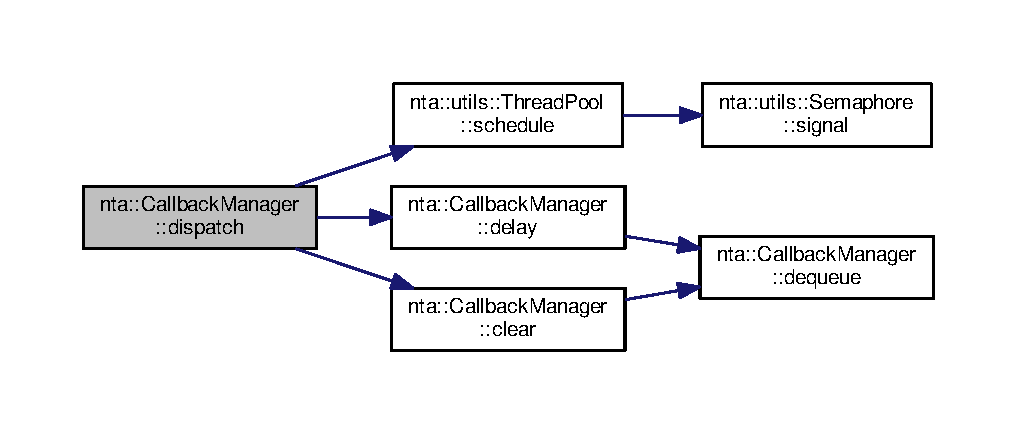
\includegraphics[width=350pt]{d1/de6/classnta_1_1CallbackManager_a7912dc908d7a7a44267ddd8fa6fb8686_cgraph}
\end{center}
\end{figure}
Here is the caller graph for this function\+:\nopagebreak
\begin{figure}[H]
\begin{center}
\leavevmode
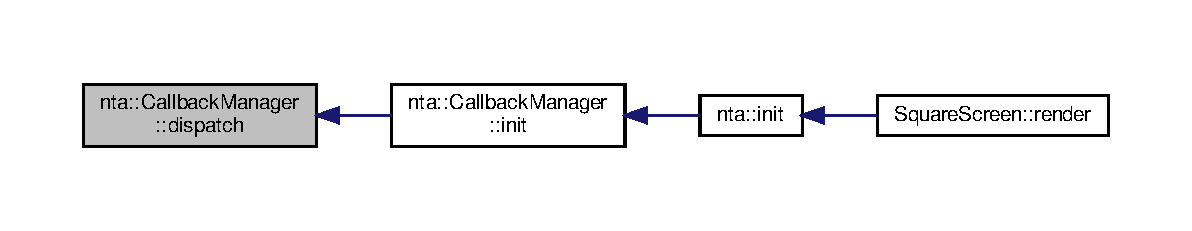
\includegraphics[width=340pt]{d1/de6/classnta_1_1CallbackManager_a7912dc908d7a7a44267ddd8fa6fb8686_icgraph}
\end{center}
\end{figure}
\mbox{\Hypertarget{classnta_1_1CallbackManager_a1fd6132e79e49dbcb787bc8a8507a931}\label{classnta_1_1CallbackManager_a1fd6132e79e49dbcb787bc8a8507a931}} 
\index{nta\+::\+Callback\+Manager@{nta\+::\+Callback\+Manager}!set\+Interval@{set\+Interval}}
\index{set\+Interval@{set\+Interval}!nta\+::\+Callback\+Manager@{nta\+::\+Callback\+Manager}}
\subsubsection{\texorpdfstring{set\+Interval()}{setInterval()}}
{\footnotesize\ttfamily uint64\+\_\+t nta\+::\+Callback\+Manager\+::set\+Interval (\begin{DoxyParamCaption}\item[{const Thunk \&}]{thunk,  }\item[{uint64\+\_\+t}]{when,  }\item[{uint64\+\_\+t}]{period }\end{DoxyParamCaption})\hspace{0.3cm}{\ttfamily [static]}}

Schedules a function to be called after when frames and then repeatedly after each subsequent period frames 

Definition at line 15 of file Callback\+Manager.\+cpp.



Referenced by set\+Timeout().

Here is the caller graph for this function\+:\nopagebreak
\begin{figure}[H]
\begin{center}
\leavevmode
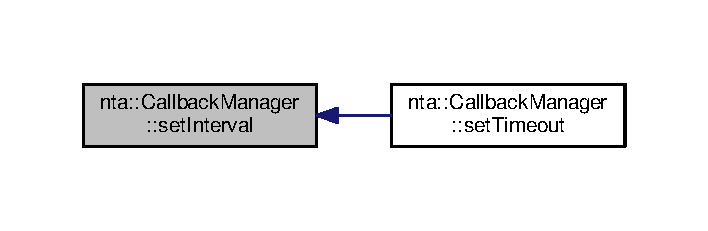
\includegraphics[width=340pt]{d1/de6/classnta_1_1CallbackManager_a1fd6132e79e49dbcb787bc8a8507a931_icgraph}
\end{center}
\end{figure}


The documentation for this class was generated from the following files\+:\begin{DoxyCompactItemize}
\item 
include/nta/Callback\+Manager.\+h\item 
src/Callback\+Manager.\+cpp\end{DoxyCompactItemize}

\hypertarget{classnta_1_1Camera2D}{}\section{nta\+:\+:Camera2D Class Reference}
\label{classnta_1_1Camera2D}\index{nta\+::\+Camera2D@{nta\+::\+Camera2D}}


{\ttfamily \#include $<$Camera2\+D.\+h$>$}

\subsection*{Public Member Functions}
\begin{DoxyCompactItemize}
\item 
\hyperlink{classnta_1_1Camera2D_a11aada3f997c594ade11dd3c46d826f4}{Camera2D} ()
\item 
\mbox{\Hypertarget{classnta_1_1Camera2D_a69171de8322165de5f134a83e33c419a}\label{classnta_1_1Camera2D_a69171de8322165de5f134a83e33c419a}} 
{\bfseries Camera2D} (crvec2 center)
\item 
\mbox{\Hypertarget{classnta_1_1Camera2D_af503a21cf73859010aefbacb1af7078c}\label{classnta_1_1Camera2D_af503a21cf73859010aefbacb1af7078c}} 
{\bfseries Camera2D} (crvec2 center, crvec2 dimensions)
\item 
\mbox{\Hypertarget{classnta_1_1Camera2D_a455d4862168f1dc4fe81040d6fcc80d2}\label{classnta_1_1Camera2D_a455d4862168f1dc4fe81040d6fcc80d2}} 
{\bfseries Camera2D} (crvec2 center, crvec2 dimensions, float orientation)
\item 
\mbox{\Hypertarget{classnta_1_1Camera2D_a18046ff230e055a06c6ca750e6eea8de}\label{classnta_1_1Camera2D_a18046ff230e055a06c6ca750e6eea8de}} 
\hyperlink{classnta_1_1Camera2D_a18046ff230e055a06c6ca750e6eea8de}{$\sim$\+Camera2D} ()
\begin{DoxyCompactList}\small\item\em destructor \end{DoxyCompactList}\item 
\mbox{\Hypertarget{classnta_1_1Camera2D_a5bbd89d9119dcd820e60756b816ad0b3}\label{classnta_1_1Camera2D_a5bbd89d9119dcd820e60756b816ad0b3}} 
glm\+::mat3 \hyperlink{classnta_1_1Camera2D_a5bbd89d9119dcd820e60756b816ad0b3}{get\+Translation\+Matrix} () const
\begin{DoxyCompactList}\small\item\em returns the 3x3 matrix representing the camera\textquotesingle{}s view \end{DoxyCompactList}\item 
\mbox{\Hypertarget{classnta_1_1Camera2D_ab3fb29b12f0b118dd2be95f701b81e2f}\label{classnta_1_1Camera2D_ab3fb29b12f0b118dd2be95f701b81e2f}} 
glm\+::mat3 {\bfseries get\+Rotation\+Matrix} () const
\item 
\mbox{\Hypertarget{classnta_1_1Camera2D_a5b28e343c69aa1f7ded1b8416e556e21}\label{classnta_1_1Camera2D_a5b28e343c69aa1f7ded1b8416e556e21}} 
glm\+::mat3 {\bfseries get\+Inverse\+Rotation\+Matrix} () const
\item 
\mbox{\Hypertarget{classnta_1_1Camera2D_a685dbe2ddad68666132fbf1edec932a6}\label{classnta_1_1Camera2D_a685dbe2ddad68666132fbf1edec932a6}} 
glm\+::mat3 {\bfseries get\+Dilation\+Matrix} () const
\item 
\mbox{\Hypertarget{classnta_1_1Camera2D_a203daa81f32279e969de57a549165297}\label{classnta_1_1Camera2D_a203daa81f32279e969de57a549165297}} 
glm\+::mat3 {\bfseries get\+Camera\+Matrix} () const
\item 
\mbox{\Hypertarget{classnta_1_1Camera2D_ad02d4b9a995f3919c753fd2ea6d9f8f1}\label{classnta_1_1Camera2D_ad02d4b9a995f3919c753fd2ea6d9f8f1}} 
glm\+::vec4 \hyperlink{classnta_1_1Camera2D_ad02d4b9a995f3919c753fd2ea6d9f8f1}{get\+Bounds\+Center} () const
\begin{DoxyCompactList}\small\item\em returns camera bounds in the given format \end{DoxyCompactList}\item 
\mbox{\Hypertarget{classnta_1_1Camera2D_af3b971aa62c8e6ca7287d0d236bb3e3d}\label{classnta_1_1Camera2D_af3b971aa62c8e6ca7287d0d236bb3e3d}} 
glm\+::vec4 {\bfseries get\+Bounds\+Top\+Left} () const
\item 
\mbox{\Hypertarget{classnta_1_1Camera2D_add5061ade3ed4eb82d3e75f6aba97f70}\label{classnta_1_1Camera2D_add5061ade3ed4eb82d3e75f6aba97f70}} 
glm\+::vec2 \hyperlink{classnta_1_1Camera2D_add5061ade3ed4eb82d3e75f6aba97f70}{get\+Center} () const
\begin{DoxyCompactList}\small\item\em returns the center, top left coordinate, and dimensions of the camera\textquotesingle{}s view \end{DoxyCompactList}\item 
\mbox{\Hypertarget{classnta_1_1Camera2D_adbfd52308be6b9c56736400ac67b65c5}\label{classnta_1_1Camera2D_adbfd52308be6b9c56736400ac67b65c5}} 
glm\+::vec2 {\bfseries get\+Top\+Left} () const
\item 
\mbox{\Hypertarget{classnta_1_1Camera2D_a2f688f531a999d2b427ef63a18859e6d}\label{classnta_1_1Camera2D_a2f688f531a999d2b427ef63a18859e6d}} 
glm\+::vec2 {\bfseries get\+Dimensions} () const
\item 
\mbox{\Hypertarget{classnta_1_1Camera2D_a6b3b7c18d66f680c05087b94214bc98f}\label{classnta_1_1Camera2D_a6b3b7c18d66f680c05087b94214bc98f}} 
glm\+::vec2 {\bfseries get\+Rotated\+Dimensions} () const
\item 
\mbox{\Hypertarget{classnta_1_1Camera2D_a5cf5e5e022f29952af085a63980e737c}\label{classnta_1_1Camera2D_a5cf5e5e022f29952af085a63980e737c}} 
float {\bfseries get\+Orientation} () const
\item 
\mbox{\Hypertarget{classnta_1_1Camera2D_a395b5bfa81b603a3d4e78d6c54aa8212}\label{classnta_1_1Camera2D_a395b5bfa81b603a3d4e78d6c54aa8212}} 
std\+::tuple$<$ glm\+::vec2, glm\+::vec2 $>$ \hyperlink{classnta_1_1Camera2D_a395b5bfa81b603a3d4e78d6c54aa8212}{get\+Axes} () const
\begin{DoxyCompactList}\small\item\em returns (normalized) axes aligned with the camera \end{DoxyCompactList}\item 
\mbox{\Hypertarget{classnta_1_1Camera2D_afb20fb9823724babdc8d18b17336169c}\label{classnta_1_1Camera2D_afb20fb9823724babdc8d18b17336169c}} 
glm\+::vec2 \hyperlink{classnta_1_1Camera2D_afb20fb9823724babdc8d18b17336169c}{mouse\+To\+Game} (crvec2 mouse, crvec2 window\+Dimensions) const
\begin{DoxyCompactList}\small\item\em converts mouse coordinates to world coordinates \end{DoxyCompactList}\item 
\mbox{\Hypertarget{classnta_1_1Camera2D_a11a7edceed0964b375fbfe154b9a9895}\label{classnta_1_1Camera2D_a11a7edceed0964b375fbfe154b9a9895}} 
void \hyperlink{classnta_1_1Camera2D_a11a7edceed0964b375fbfe154b9a9895}{set\+Center} (crvec2 center)
\begin{DoxyCompactList}\small\item\em sets the values of the camera\textquotesingle{}s fields \end{DoxyCompactList}\item 
\mbox{\Hypertarget{classnta_1_1Camera2D_a5e887ee36c95789e3455ab2f3bb3f568}\label{classnta_1_1Camera2D_a5e887ee36c95789e3455ab2f3bb3f568}} 
void {\bfseries set\+Center} (float x, float y)
\item 
\mbox{\Hypertarget{classnta_1_1Camera2D_a3b133bef64504b488b04ce18e206544b}\label{classnta_1_1Camera2D_a3b133bef64504b488b04ce18e206544b}} 
void {\bfseries set\+Dimensions} (crvec2 dimensions)
\item 
\mbox{\Hypertarget{classnta_1_1Camera2D_a253821b9dc464678c80ff92c31a8689f}\label{classnta_1_1Camera2D_a253821b9dc464678c80ff92c31a8689f}} 
void {\bfseries set\+Dimensions} (float w, float h)
\item 
\mbox{\Hypertarget{classnta_1_1Camera2D_ae1b3a5ef4259881936317fc0c18c4a13}\label{classnta_1_1Camera2D_ae1b3a5ef4259881936317fc0c18c4a13}} 
void {\bfseries set\+Orientation} (float t)
\item 
void \hyperlink{classnta_1_1Camera2D_a711b1b64b4e0bbca5c598ac15609f498}{translate\+Center} (crvec2 translation, bool move\+\_\+along\+\_\+axes=false)
\item 
\mbox{\Hypertarget{classnta_1_1Camera2D_a95ecd50d9ec6031b4d015f33d442d096}\label{classnta_1_1Camera2D_a95ecd50d9ec6031b4d015f33d442d096}} 
void {\bfseries translate\+Center} (float dx, float dy, bool move\+\_\+along\+\_\+axes=false)
\item 
\mbox{\Hypertarget{classnta_1_1Camera2D_aa89b58a2a5ca0c3df56d07e2722afcd6}\label{classnta_1_1Camera2D_aa89b58a2a5ca0c3df56d07e2722afcd6}} 
void \hyperlink{classnta_1_1Camera2D_aa89b58a2a5ca0c3df56d07e2722afcd6}{scale\+Dimensions} (crvec2 dilation)
\begin{DoxyCompactList}\small\item\em scales the camera\textquotesingle{}s field of view \end{DoxyCompactList}\item 
\mbox{\Hypertarget{classnta_1_1Camera2D_ae5e80a376fe4b6457e712c6bc94b8584}\label{classnta_1_1Camera2D_ae5e80a376fe4b6457e712c6bc94b8584}} 
void {\bfseries scale\+Dimensions} (float dw, float dh)
\item 
\mbox{\Hypertarget{classnta_1_1Camera2D_a4529f2111c2621764c42365df5a504e0}\label{classnta_1_1Camera2D_a4529f2111c2621764c42365df5a504e0}} 
void \hyperlink{classnta_1_1Camera2D_a4529f2111c2621764c42365df5a504e0}{rotate} (float dt)
\begin{DoxyCompactList}\small\item\em rotates the camera \end{DoxyCompactList}\end{DoxyCompactItemize}
\subsection*{Private Attributes}
\begin{DoxyCompactItemize}
\item 
\mbox{\Hypertarget{classnta_1_1Camera2D_a6f63c871727ef4037b164be0b400cd89}\label{classnta_1_1Camera2D_a6f63c871727ef4037b164be0b400cd89}} 
glm\+::vec2 \hyperlink{classnta_1_1Camera2D_a6f63c871727ef4037b164be0b400cd89}{m\+\_\+center}
\begin{DoxyCompactList}\small\item\em center of the camera\textquotesingle{}s view in world coordinates \end{DoxyCompactList}\item 
\mbox{\Hypertarget{classnta_1_1Camera2D_a403ec8d18fd31d5164ba81267cca555e}\label{classnta_1_1Camera2D_a403ec8d18fd31d5164ba81267cca555e}} 
glm\+::vec2 \hyperlink{classnta_1_1Camera2D_a403ec8d18fd31d5164ba81267cca555e}{m\+\_\+dimensions}
\begin{DoxyCompactList}\small\item\em half dimensions of camera\textquotesingle{}s view in world coordinates \end{DoxyCompactList}\item 
\mbox{\Hypertarget{classnta_1_1Camera2D_abdec8877a0bf8cf0ad6c74440aa18eb4}\label{classnta_1_1Camera2D_abdec8877a0bf8cf0ad6c74440aa18eb4}} 
float \hyperlink{classnta_1_1Camera2D_abdec8877a0bf8cf0ad6c74440aa18eb4}{m\+\_\+orientation}
\begin{DoxyCompactList}\small\item\em rotation about axis orthogonal to the world \end{DoxyCompactList}\end{DoxyCompactItemize}


\subsection{Detailed Description}
represents a camera in two dimensions from which the world is viewed

You can imagine the 2D world is flat against the wall, and this camera is facing that wall. You can move the camera in space (i.\+e. set\+Center/set\+Dimensions), and it can be rotated about an axis orthogonal to the world, through its center. 

Definition at line 12 of file Camera2\+D.\+h.



\subsection{Constructor \& Destructor Documentation}
\mbox{\Hypertarget{classnta_1_1Camera2D_a11aada3f997c594ade11dd3c46d826f4}\label{classnta_1_1Camera2D_a11aada3f997c594ade11dd3c46d826f4}} 
\index{nta\+::\+Camera2D@{nta\+::\+Camera2D}!Camera2D@{Camera2D}}
\index{Camera2D@{Camera2D}!nta\+::\+Camera2D@{nta\+::\+Camera2D}}
\subsubsection{\texorpdfstring{Camera2\+D()}{Camera2D()}}
{\footnotesize\ttfamily nta\+::\+Camera2\+D\+::\+Camera2D (\begin{DoxyParamCaption}{ }\end{DoxyParamCaption})}

Constructs a new \hyperlink{classnta_1_1Camera2D}{Camera2D}. By default, the center is at (0,0), the dimensions are (100, 100), and orientation is 0 

Definition at line 4 of file Camera2\+D.\+cpp.



\subsection{Member Function Documentation}
\mbox{\Hypertarget{classnta_1_1Camera2D_a711b1b64b4e0bbca5c598ac15609f498}\label{classnta_1_1Camera2D_a711b1b64b4e0bbca5c598ac15609f498}} 
\index{nta\+::\+Camera2D@{nta\+::\+Camera2D}!translate\+Center@{translate\+Center}}
\index{translate\+Center@{translate\+Center}!nta\+::\+Camera2D@{nta\+::\+Camera2D}}
\subsubsection{\texorpdfstring{translate\+Center()}{translateCenter()}}
{\footnotesize\ttfamily void nta\+::\+Camera2\+D\+::translate\+Center (\begin{DoxyParamCaption}\item[{crvec2}]{translation,  }\item[{bool}]{move\+\_\+along\+\_\+axes = {\ttfamily false} }\end{DoxyParamCaption})}

moves the camera around the world By default, if the world is rotated, it does not move along the rotated axes 

Definition at line 114 of file Camera2\+D.\+cpp.



The documentation for this class was generated from the following files\+:\begin{DoxyCompactItemize}
\item 
include/nta/Camera2\+D.\+h\item 
src/Camera2\+D.\+cpp\end{DoxyCompactItemize}

\hypertarget{structnta_1_1FontMap_1_1CharRect}{}\section{nta\+:\+:Font\+Map\+:\+:Char\+Rect Struct Reference}
\label{structnta_1_1FontMap_1_1CharRect}\index{nta\+::\+Font\+Map\+::\+Char\+Rect@{nta\+::\+Font\+Map\+::\+Char\+Rect}}


a rectangle representing the location of a char in the \hyperlink{classnta_1_1FontMap}{Font\+Map}  


\subsection*{Public Member Functions}
\begin{DoxyCompactItemize}
\item 
\mbox{\Hypertarget{structnta_1_1FontMap_1_1CharRect_aae578d461eba96e8fbf71f507b99a87f}\label{structnta_1_1FontMap_1_1CharRect_aae578d461eba96e8fbf71f507b99a87f}} 
{\bfseries Char\+Rect} (glm\+::vec2 tl, glm\+::vec2 d, bool a)
\end{DoxyCompactItemize}
\subsection*{Public Attributes}
\begin{DoxyCompactItemize}
\item 
\mbox{\Hypertarget{structnta_1_1FontMap_1_1CharRect_a84c89136099916d5e825d487fec1fd50}\label{structnta_1_1FontMap_1_1CharRect_a84c89136099916d5e825d487fec1fd50}} 
glm\+::vec2 {\bfseries top\+Left}
\item 
\mbox{\Hypertarget{structnta_1_1FontMap_1_1CharRect_a3f5d24fdc091d334c532274b9a79fd0d}\label{structnta_1_1FontMap_1_1CharRect_a3f5d24fdc091d334c532274b9a79fd0d}} 
glm\+::vec2 {\bfseries dimensions}
\item 
\mbox{\Hypertarget{structnta_1_1FontMap_1_1CharRect_a605388f5ce8e4e7316276d9b0df740cb}\label{structnta_1_1FontMap_1_1CharRect_a605388f5ce8e4e7316276d9b0df740cb}} 
bool {\bfseries added\+To\+Map}
\end{DoxyCompactItemize}


\subsection{Detailed Description}
a rectangle representing the location of a char in the \hyperlink{classnta_1_1FontMap}{Font\+Map} 

Definition at line 26 of file Sprite\+Font.\+h.



Collaboration diagram for nta\+:\+:Font\+Map\+:\+:Char\+Rect\+:
\nopagebreak
\begin{figure}[H]
\begin{center}
\leavevmode
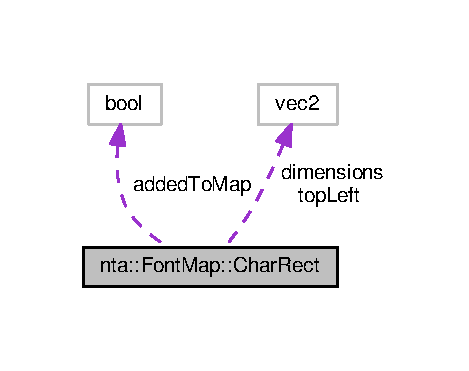
\includegraphics[width=225pt]{de/df1/structnta_1_1FontMap_1_1CharRect__coll__graph}
\end{center}
\end{figure}


The documentation for this struct was generated from the following file\+:\begin{DoxyCompactItemize}
\item 
include/nta/Sprite\+Font.\+h\end{DoxyCompactItemize}

\hypertarget{classnta_1_1Compressor}{}\section{nta\+:\+:Compressor Class Reference}
\label{classnta_1_1Compressor}\index{nta\+::\+Compressor@{nta\+::\+Compressor}}


Static class for compressing byte buffers.  




{\ttfamily \#include $<$Compressor.\+h$>$}

\subsection*{Static Public Member Functions}
\begin{DoxyCompactItemize}
\item 
\mbox{\Hypertarget{classnta_1_1Compressor_aaf2c8b87946d2cee8b4edcf4c48f7f71}\label{classnta_1_1Compressor_aaf2c8b87946d2cee8b4edcf4c48f7f71}} 
static std\+::vector$<$ G\+Lubyte $>$ \hyperlink{classnta_1_1Compressor_aaf2c8b87946d2cee8b4edcf4c48f7f71}{decompress} (const std\+::vector$<$ G\+Lubyte $>$ \&data)
\begin{DoxyCompactList}\small\item\em decompressed data that was compressed by this class \end{DoxyCompactList}\item 
\mbox{\Hypertarget{classnta_1_1Compressor_ac5f5822b598309d4ef6a89edb7bdcf10}\label{classnta_1_1Compressor_ac5f5822b598309d4ef6a89edb7bdcf10}} 
static std\+::vector$<$ G\+Lubyte $>$ \hyperlink{classnta_1_1Compressor_ac5f5822b598309d4ef6a89edb7bdcf10}{compress} (const std\+::vector$<$ G\+Lubyte $>$ \&data)
\begin{DoxyCompactList}\small\item\em compresses a bye buffer \end{DoxyCompactList}\end{DoxyCompactItemize}
\subsection*{Static Private Member Functions}
\begin{DoxyCompactItemize}
\item 
\mbox{\Hypertarget{classnta_1_1Compressor_affed498c6ed43db813de5c46892b9163}\label{classnta_1_1Compressor_affed498c6ed43db813de5c46892b9163}} 
static std\+::string \hyperlink{classnta_1_1Compressor_affed498c6ed43db813de5c46892b9163}{to\+Binary} (int num, int num\+Bits=8)
\begin{DoxyCompactList}\small\item\em converts number to its binary representation \end{DoxyCompactList}\item 
\mbox{\Hypertarget{classnta_1_1Compressor_aa7950ec19d7beda1b1102d1df453861f}\label{classnta_1_1Compressor_aa7950ec19d7beda1b1102d1df453861f}} 
static int \hyperlink{classnta_1_1Compressor_aa7950ec19d7beda1b1102d1df453861f}{from\+Binary} (crstring num)
\begin{DoxyCompactList}\small\item\em reads a binary number from a string \end{DoxyCompactList}\item 
\mbox{\Hypertarget{classnta_1_1Compressor_ade1d9da3d6a4ccc45fb17a83f9d7c4ed}\label{classnta_1_1Compressor_ade1d9da3d6a4ccc45fb17a83f9d7c4ed}} 
static void \hyperlink{classnta_1_1Compressor_ade1d9da3d6a4ccc45fb17a83f9d7c4ed}{create\+Tree} (const std\+::vector$<$ G\+Lubyte $>$ \&data)
\begin{DoxyCompactList}\small\item\em creates a Huffman tree from a buffer \end{DoxyCompactList}\end{DoxyCompactItemize}
\subsection*{Static Private Attributes}
\begin{DoxyCompactItemize}
\item 
\mbox{\Hypertarget{classnta_1_1Compressor_a85e378612ff069d0bc915c87fae74e7d}\label{classnta_1_1Compressor_a85e378612ff069d0bc915c87fae74e7d}} 
static std\+::map$<$ G\+Lubyte, std\+::string $>$ \hyperlink{classnta_1_1Compressor_a85e378612ff069d0bc915c87fae74e7d}{m\+\_\+encodings}
\begin{DoxyCompactList}\small\item\em the encodings generated from the tree \end{DoxyCompactList}\item 
\mbox{\Hypertarget{classnta_1_1Compressor_a9cec9a631892c8cd4b9c2358c7ac41f4}\label{classnta_1_1Compressor_a9cec9a631892c8cd4b9c2358c7ac41f4}} 
static \hyperlink{classnta_1_1HuffmanNode}{Huffman\+Node} $\ast$ \hyperlink{classnta_1_1Compressor_a9cec9a631892c8cd4b9c2358c7ac41f4}{m\+\_\+root}
\begin{DoxyCompactList}\small\item\em the root of the created Huffman tree \end{DoxyCompactList}\end{DoxyCompactItemize}


\subsection{Detailed Description}
Static class for compressing byte buffers. 

Definition at line 53 of file Compressor.\+h.



The documentation for this class was generated from the following files\+:\begin{DoxyCompactItemize}
\item 
include/nta/Compressor.\+h\item 
src/Compressor.\+cpp\end{DoxyCompactItemize}

\hypertarget{classnta_1_1DebugBatch}{}\section{nta\+:\+:Debug\+Batch Class Reference}
\label{classnta_1_1DebugBatch}\index{nta\+::\+Debug\+Batch@{nta\+::\+Debug\+Batch}}


A collection of debug primitives (outlines of shapes) to be drawn.  




{\ttfamily \#include $<$Debug\+Batch.\+h$>$}

\subsection*{Public Member Functions}
\begin{DoxyCompactItemize}
\item 
\mbox{\Hypertarget{classnta_1_1DebugBatch_ab546a069bab54be8d89a3937f418292e}\label{classnta_1_1DebugBatch_ab546a069bab54be8d89a3937f418292e}} 
\hyperlink{classnta_1_1DebugBatch_ab546a069bab54be8d89a3937f418292e}{Debug\+Batch} ()
\begin{DoxyCompactList}\small\item\em Constructor. Doesn\textquotesingle{}t actually do anything; use \hyperlink{classnta_1_1DebugBatch_a9d60f69ba86c7267e69984cc29e1f53c}{init()} to initialize instead. \end{DoxyCompactList}\item 
\mbox{\Hypertarget{classnta_1_1DebugBatch_a9d60f69ba86c7267e69984cc29e1f53c}\label{classnta_1_1DebugBatch_a9d60f69ba86c7267e69984cc29e1f53c}} 
void \hyperlink{classnta_1_1DebugBatch_a9d60f69ba86c7267e69984cc29e1f53c}{init} ()
\begin{DoxyCompactList}\small\item\em initializes the batch (only needs to be called once) \end{DoxyCompactList}\item 
\mbox{\Hypertarget{classnta_1_1DebugBatch_a183ea86f6636aef3aeae66a0eb8aec5a}\label{classnta_1_1DebugBatch_a183ea86f6636aef3aeae66a0eb8aec5a}} 
void \hyperlink{classnta_1_1DebugBatch_a183ea86f6636aef3aeae66a0eb8aec5a}{begin} ()
\begin{DoxyCompactList}\small\item\em begins collecting shapes to be drawn \end{DoxyCompactList}\item 
\mbox{\Hypertarget{classnta_1_1DebugBatch_abc2f517c6dd1fb4a65624335d11c92f1}\label{classnta_1_1DebugBatch_abc2f517c6dd1fb4a65624335d11c92f1}} 
void \hyperlink{classnta_1_1DebugBatch_abc2f517c6dd1fb4a65624335d11c92f1}{end} ()
\begin{DoxyCompactList}\small\item\em ends collecting shapes \end{DoxyCompactList}\item 
\mbox{\Hypertarget{classnta_1_1DebugBatch_abc7c94706f334db36992b486885868a2}\label{classnta_1_1DebugBatch_abc7c94706f334db36992b486885868a2}} 
void \hyperlink{classnta_1_1DebugBatch_abc7c94706f334db36992b486885868a2}{add\+Line} (crvec2 start, crvec2 \hyperlink{classnta_1_1DebugBatch_abc2f517c6dd1fb4a65624335d11c92f1}{end}, crvec4 color=glm\+::vec4(1), int num\+\_\+pieces=2)
\begin{DoxyCompactList}\small\item\em Adds a shape to the batch. \end{DoxyCompactList}\item 
\mbox{\Hypertarget{classnta_1_1DebugBatch_aeb4dbbdb8501560147df6ae3c37f706e}\label{classnta_1_1DebugBatch_aeb4dbbdb8501560147df6ae3c37f706e}} 
void {\bfseries add\+Line} (crvec2 start, crvec2 \hyperlink{classnta_1_1DebugBatch_abc2f517c6dd1fb4a65624335d11c92f1}{end}, int num\+\_\+pieces, crvec4 color=glm\+::vec4(1))
\item 
\mbox{\Hypertarget{classnta_1_1DebugBatch_afd4376b4d4532995c7a7ca2766627d48}\label{classnta_1_1DebugBatch_afd4376b4d4532995c7a7ca2766627d48}} 
void {\bfseries add\+Rect} (crvec4 pos\+Rect, crvec4 color=glm\+::vec4(1), float orientation=0)
\item 
\mbox{\Hypertarget{classnta_1_1DebugBatch_a8b83a2974e7eaaa5bca4bd8038bda51d}\label{classnta_1_1DebugBatch_a8b83a2974e7eaaa5bca4bd8038bda51d}} 
void {\bfseries add\+Rect} (crvec4 pos\+Rect, float orientation, crvec4 color=glm\+::vec4(1))
\item 
\mbox{\Hypertarget{classnta_1_1DebugBatch_a15f5ca4fb6f93d67c417795b5aa8a255}\label{classnta_1_1DebugBatch_a15f5ca4fb6f93d67c417795b5aa8a255}} 
void {\bfseries add\+Circle} (crvec2 center, float radius, crvec4 color=glm\+::vec4(1))
\item 
\mbox{\Hypertarget{classnta_1_1DebugBatch_af610dfb8caf64615bc14cd96eee2a432}\label{classnta_1_1DebugBatch_af610dfb8caf64615bc14cd96eee2a432}} 
void {\bfseries add\+Polygon} (std\+::size\+\_\+t num\+Sides, crvec2 center, float side\+Length, float orientation, crvec4 color=glm\+::vec4(1))
\item 
\mbox{\Hypertarget{classnta_1_1DebugBatch_a3188990f4fd9aeede13573fe00bd0cf4}\label{classnta_1_1DebugBatch_a3188990f4fd9aeede13573fe00bd0cf4}} 
void \hyperlink{classnta_1_1DebugBatch_a3188990f4fd9aeede13573fe00bd0cf4}{render} () const
\begin{DoxyCompactList}\small\item\em renders the batch \end{DoxyCompactList}\end{DoxyCompactItemize}
\subsection*{Private Attributes}
\begin{DoxyCompactItemize}
\item 
\mbox{\Hypertarget{classnta_1_1DebugBatch_a7c699660499350f5717a13dc2266cd9c}\label{classnta_1_1DebugBatch_a7c699660499350f5717a13dc2266cd9c}} 
std\+::vector$<$ \hyperlink{structnta_1_1Vertex2D}{Vertex2D} $>$ {\bfseries m\+\_\+vertices}
\item 
\mbox{\Hypertarget{classnta_1_1DebugBatch_a1c0359676583c9c60d29b74b909939ee}\label{classnta_1_1DebugBatch_a1c0359676583c9c60d29b74b909939ee}} 
std\+::vector$<$ G\+Luint $>$ {\bfseries m\+\_\+indices}
\item 
\mbox{\Hypertarget{classnta_1_1DebugBatch_a13089a13e5a589c9185c566e2957d0b5}\label{classnta_1_1DebugBatch_a13089a13e5a589c9185c566e2957d0b5}} 
G\+Luint {\bfseries m\+\_\+vao} = 0
\item 
\mbox{\Hypertarget{classnta_1_1DebugBatch_a8d3d799f71618a40d9403eda7f62a7de}\label{classnta_1_1DebugBatch_a8d3d799f71618a40d9403eda7f62a7de}} 
G\+Luint {\bfseries m\+\_\+vbo} = 0
\item 
\mbox{\Hypertarget{classnta_1_1DebugBatch_ae85fcc91c2121dd5e438e73dfdf2c638}\label{classnta_1_1DebugBatch_ae85fcc91c2121dd5e438e73dfdf2c638}} 
G\+Luint {\bfseries m\+\_\+ibo} = 0
\end{DoxyCompactItemize}


\subsection{Detailed Description}
A collection of debug primitives (outlines of shapes) to be drawn. 

Definition at line 12 of file Debug\+Batch.\+h.



Collaboration diagram for nta\+:\+:Debug\+Batch\+:\nopagebreak
\begin{figure}[H]
\begin{center}
\leavevmode
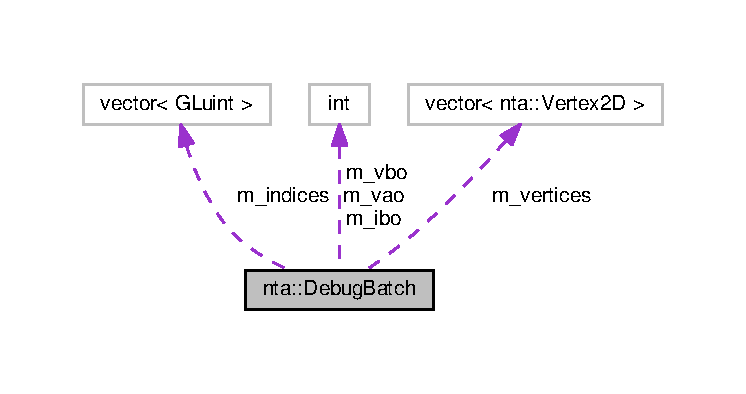
\includegraphics[width=350pt]{db/d88/classnta_1_1DebugBatch__coll__graph}
\end{center}
\end{figure}


The documentation for this class was generated from the following files\+:\begin{DoxyCompactItemize}
\item 
include/nta/Debug\+Batch.\+h\item 
src/Debug\+Batch.\+cpp\end{DoxyCompactItemize}

\hypertarget{structnta_1_1Error}{}\section{nta\+:\+:Error Struct Reference}
\label{structnta_1_1Error}\index{nta\+::\+Error@{nta\+::\+Error}}


Something went wrong.  




{\ttfamily \#include $<$Errors.\+h$>$}

\subsection*{Public Member Functions}
\begin{DoxyCompactItemize}
\item 
\mbox{\Hypertarget{structnta_1_1Error_a6239093a37e2bd25278da1f2be70bcdc}\label{structnta_1_1Error_a6239093a37e2bd25278da1f2be70bcdc}} 
{\bfseries Error} (crstring desc=\char`\"{}\char`\"{}, \hyperlink{namespacenta_a1ddeff35318678e360dfa44ca9577b16}{Error\+Type} t=O\+T\+H\+ER)
\item 
\mbox{\Hypertarget{structnta_1_1Error_a128f41302dac9b5e1e2b783588b6cb28}\label{structnta_1_1Error_a128f41302dac9b5e1e2b783588b6cb28}} 
{\bfseries Error} (const \hyperlink{structnta_1_1Error}{Error} \&other)
\end{DoxyCompactItemize}
\subsection*{Public Attributes}
\begin{DoxyCompactItemize}
\item 
\mbox{\Hypertarget{structnta_1_1Error_afd857a214f99264d095d42fcf076318b}\label{structnta_1_1Error_afd857a214f99264d095d42fcf076318b}} 
std\+::string \hyperlink{structnta_1_1Error_afd857a214f99264d095d42fcf076318b}{description}
\begin{DoxyCompactList}\small\item\em A description of what when wrong. \end{DoxyCompactList}\item 
\mbox{\Hypertarget{structnta_1_1Error_a7bc9638dee4444ef9306b83a889d4257}\label{structnta_1_1Error_a7bc9638dee4444ef9306b83a889d4257}} 
\hyperlink{namespacenta_a1ddeff35318678e360dfa44ca9577b16}{Error\+Type} \hyperlink{structnta_1_1Error_a7bc9638dee4444ef9306b83a889d4257}{type}
\begin{DoxyCompactList}\small\item\em The type of error that occured. \end{DoxyCompactList}\item 
\mbox{\Hypertarget{structnta_1_1Error_a56fe79b4b8e915fa60f580ca80cc4ed7}\label{structnta_1_1Error_a56fe79b4b8e915fa60f580ca80cc4ed7}} 
const \hyperlink{structnta_1_1Error}{Error} $\ast$ \hyperlink{structnta_1_1Error_a56fe79b4b8e915fa60f580ca80cc4ed7}{prev} = nullptr
\begin{DoxyCompactList}\small\item\em The most recent unhandled error before this one. \end{DoxyCompactList}\end{DoxyCompactItemize}


\subsection{Detailed Description}
Something went wrong. 

Definition at line 23 of file Errors.\+h.



Collaboration diagram for nta\+:\+:Error\+:\nopagebreak
\begin{figure}[H]
\begin{center}
\leavevmode
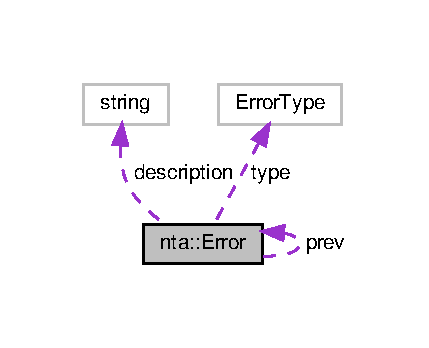
\includegraphics[width=206pt]{d7/dbb/structnta_1_1Error__coll__graph}
\end{center}
\end{figure}


The documentation for this struct was generated from the following file\+:\begin{DoxyCompactItemize}
\item 
include/nta/Errors.\+h\end{DoxyCompactItemize}

\hypertarget{classnta_1_1ErrorManager}{}\section{nta\+:\+:Error\+Manager Class Reference}
\label{classnta_1_1ErrorManager}\index{nta\+::\+Error\+Manager@{nta\+::\+Error\+Manager}}


{\ttfamily \#include $<$Errors.\+h$>$}

\subsection*{Static Public Member Functions}
\begin{DoxyCompactItemize}
\item 
\mbox{\Hypertarget{classnta_1_1ErrorManager_adca13bc3b6b36366c0a803ce43daf90d}\label{classnta_1_1ErrorManager_adca13bc3b6b36366c0a803ce43daf90d}} 
static void \hyperlink{classnta_1_1ErrorManager_adca13bc3b6b36366c0a803ce43daf90d}{handle\+\_\+errors} ()
\begin{DoxyCompactList}\small\item\em Handles all outstanding errors. \end{DoxyCompactList}\item 
\mbox{\Hypertarget{classnta_1_1ErrorManager_a7a8c3c22602b437d160e860da877fffe}\label{classnta_1_1ErrorManager_a7a8c3c22602b437d160e860da877fffe}} 
static void \hyperlink{classnta_1_1ErrorManager_a7a8c3c22602b437d160e860da877fffe}{set\+\_\+periodic\+\_\+callback} (const Error\+Callback \&callback)
\begin{DoxyCompactList}\small\item\em Sets the periodic callback function. \end{DoxyCompactList}\item 
\mbox{\Hypertarget{classnta_1_1ErrorManager_acd7eb6eafdace10701e4e59bd727a823}\label{classnta_1_1ErrorManager_acd7eb6eafdace10701e4e59bd727a823}} 
static void \hyperlink{classnta_1_1ErrorManager_acd7eb6eafdace10701e4e59bd727a823}{set\+\_\+push\+\_\+callback} (const Error\+Callback \&callback)
\begin{DoxyCompactList}\small\item\em Sets the push callback function. \end{DoxyCompactList}\item 
\mbox{\Hypertarget{classnta_1_1ErrorManager_a5e12c42f103bfa290699c08c98d681a2}\label{classnta_1_1ErrorManager_a5e12c42f103bfa290699c08c98d681a2}} 
static void \hyperlink{classnta_1_1ErrorManager_a5e12c42f103bfa290699c08c98d681a2}{push\+\_\+error} (const \hyperlink{structnta_1_1Error}{Error} \&err)
\begin{DoxyCompactList}\small\item\em Adds and error to the front of the list. \end{DoxyCompactList}\item 
\mbox{\Hypertarget{classnta_1_1ErrorManager_a42c52e9cb6537922b10b4f2546af1b7d}\label{classnta_1_1ErrorManager_a42c52e9cb6537922b10b4f2546af1b7d}} 
static const \hyperlink{structnta_1_1Error}{Error} $\ast$ \hyperlink{classnta_1_1ErrorManager_a42c52e9cb6537922b10b4f2546af1b7d}{pop\+\_\+error} ()
\begin{DoxyCompactList}\small\item\em Removes (and returns) the error from the front of the list. \end{DoxyCompactList}\item 
\mbox{\Hypertarget{classnta_1_1ErrorManager_ad156e8dea6b2a7d98d17043ec08cb812}\label{classnta_1_1ErrorManager_ad156e8dea6b2a7d98d17043ec08cb812}} 
static const \hyperlink{structnta_1_1Error}{Error} $\ast$ \hyperlink{classnta_1_1ErrorManager_ad156e8dea6b2a7d98d17043ec08cb812}{peek\+\_\+error} ()
\begin{DoxyCompactList}\small\item\em Returns the error at the front of the list. \end{DoxyCompactList}\item 
\mbox{\Hypertarget{classnta_1_1ErrorManager_a45dcc13a0acec8c4d2cc69d9b52be305}\label{classnta_1_1ErrorManager_a45dcc13a0acec8c4d2cc69d9b52be305}} 
static void \hyperlink{classnta_1_1ErrorManager_a45dcc13a0acec8c4d2cc69d9b52be305}{clear\+\_\+errors} ()
\begin{DoxyCompactList}\small\item\em Deletes all errors (without handling any of them) \end{DoxyCompactList}\end{DoxyCompactItemize}
\subsection*{Static Private Attributes}
\begin{DoxyCompactItemize}
\item 
\mbox{\Hypertarget{classnta_1_1ErrorManager_af652b22446b5ce84c85164a5ff7f30f2}\label{classnta_1_1ErrorManager_af652b22446b5ce84c85164a5ff7f30f2}} 
static const \hyperlink{structnta_1_1Error}{Error} $\ast$ \hyperlink{classnta_1_1ErrorManager_af652b22446b5ce84c85164a5ff7f30f2}{m\+\_\+errors} = nullptr
\begin{DoxyCompactList}\small\item\em A linked list of unhandled errors. \end{DoxyCompactList}\item 
\mbox{\Hypertarget{classnta_1_1ErrorManager_a26a60a2c77e97e5cf4af59bb06f20d7a}\label{classnta_1_1ErrorManager_a26a60a2c77e97e5cf4af59bb06f20d7a}} 
static Error\+Callback \hyperlink{classnta_1_1ErrorManager_a26a60a2c77e97e5cf4af59bb06f20d7a}{m\+\_\+periodic\+\_\+callback} = \mbox{[}$\,$\mbox{]}(const \hyperlink{structnta_1_1Error}{Error}$\ast$ \+\_\+) \{\}
\begin{DoxyCompactList}\small\item\em The function used to handle errors at the end of each frame. \end{DoxyCompactList}\item 
static Error\+Callback \hyperlink{classnta_1_1ErrorManager_a96ac1ed4fb4ee3dd2ca4c055ccfc630c}{m\+\_\+push\+\_\+callback}
\begin{DoxyCompactList}\small\item\em The function used to handle errors as they occur. \end{DoxyCompactList}\end{DoxyCompactItemize}


\subsection{Detailed Description}
Stores and handles Errors \begin{DoxyRefDesc}{Todo}
\item[\hyperlink{todo__todo000002}{Todo}]There should be one of each \char`\"{}\+Manager\char`\"{} class type per \hyperlink{classnta_1_1ScreenManager}{Screen\+Manager} or one per \hyperlink{classnta_1_1Window}{Window} (i.\+e. they should not be static) \end{DoxyRefDesc}


Definition at line 44 of file Errors.\+h.



Collaboration diagram for nta\+:\+:Error\+Manager\+:
\nopagebreak
\begin{figure}[H]
\begin{center}
\leavevmode
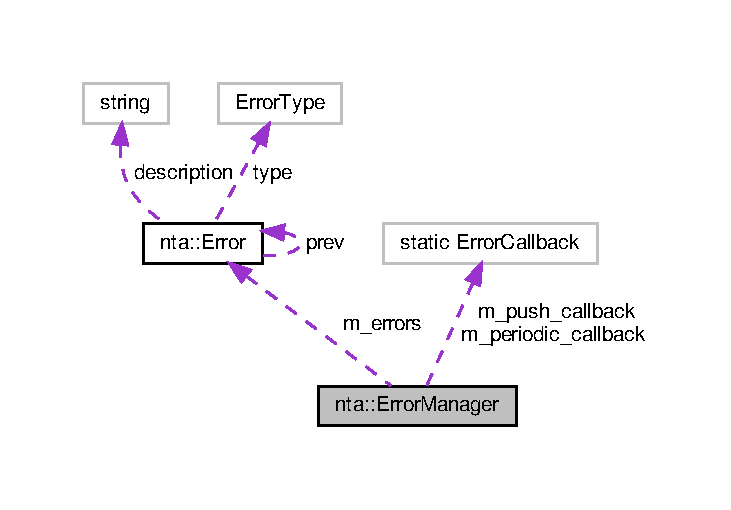
\includegraphics[width=350pt]{d5/d79/classnta_1_1ErrorManager__coll__graph}
\end{center}
\end{figure}


\subsection{Member Data Documentation}
\mbox{\Hypertarget{classnta_1_1ErrorManager_a96ac1ed4fb4ee3dd2ca4c055ccfc630c}\label{classnta_1_1ErrorManager_a96ac1ed4fb4ee3dd2ca4c055ccfc630c}} 
\index{nta\+::\+Error\+Manager@{nta\+::\+Error\+Manager}!m\+\_\+push\+\_\+callback@{m\+\_\+push\+\_\+callback}}
\index{m\+\_\+push\+\_\+callback@{m\+\_\+push\+\_\+callback}!nta\+::\+Error\+Manager@{nta\+::\+Error\+Manager}}
\subsubsection{\texorpdfstring{m\+\_\+push\+\_\+callback}{m\_push\_callback}}
{\footnotesize\ttfamily Error\+Callback nta\+::\+Error\+Manager\+::m\+\_\+push\+\_\+callback\hspace{0.3cm}{\ttfamily [static]}, {\ttfamily [private]}}

{\bfseries Initial value\+:}
\begin{DoxyCode}
= [](\textcolor{keyword}{const} Error* err) \{
        \textcolor{keywordflow}{if} (err) \{
            \hyperlink{namespacenta_a17dc16b021d0dec3749e422b95d39350}{cleanup}();
            std::cout<<\textcolor{stringliteral}{"An error occured. Check Log.log for details"}<<std::endl;
            exit(0xbad);
        \}
    \}
\end{DoxyCode}


The function used to handle errors as they occur. 



Definition at line 51 of file Errors.\+h.



Referenced by push\+\_\+error(), and set\+\_\+push\+\_\+callback().



The documentation for this class was generated from the following files\+:\begin{DoxyCompactItemize}
\item 
include/nta/Errors.\+h\item 
src/Errors.\+cpp\end{DoxyCompactItemize}

\hypertarget{classnta_1_1FontMap}{}\section{nta\+:\+:Font\+Map Class Reference}
\label{classnta_1_1FontMap}\index{nta\+::\+Font\+Map@{nta\+::\+Font\+Map}}


represents the organization of a texture containing the characters  




{\ttfamily \#include $<$Sprite\+Font.\+h$>$}



Collaboration diagram for nta\+:\+:Font\+Map\+:\nopagebreak
\begin{figure}[H]
\begin{center}
\leavevmode
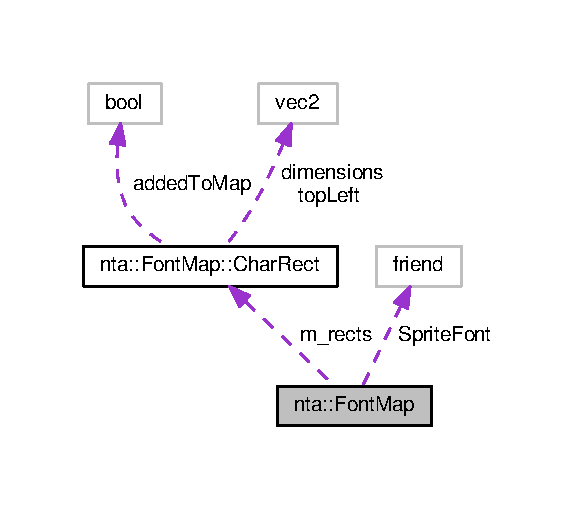
\includegraphics[width=202pt]{d3/d2b/classnta_1_1FontMap__coll__graph}
\end{center}
\end{figure}
\subsection*{Classes}
\begin{DoxyCompactItemize}
\item 
struct \hyperlink{structnta_1_1FontMap_1_1CharRect}{Char\+Rect}
\begin{DoxyCompactList}\small\item\em a rectangle representing the location of a char in the \hyperlink{classnta_1_1FontMap}{Font\+Map} \end{DoxyCompactList}\end{DoxyCompactItemize}
\subsection*{Public Member Functions}
\begin{DoxyCompactItemize}
\item 
\mbox{\Hypertarget{classnta_1_1FontMap_a1839735db2d53428126d3381dc7f3928}\label{classnta_1_1FontMap_a1839735db2d53428126d3381dc7f3928}} 
\hyperlink{classnta_1_1FontMap_a1839735db2d53428126d3381dc7f3928}{Font\+Map} ()
\begin{DoxyCompactList}\small\item\em constructor and destructor \end{DoxyCompactList}\item 
\mbox{\Hypertarget{classnta_1_1FontMap_a3e51706b5955f482f776b0d6980750b3}\label{classnta_1_1FontMap_a3e51706b5955f482f776b0d6980750b3}} 
glm\+::vec2 \hyperlink{classnta_1_1FontMap_a3e51706b5955f482f776b0d6980750b3}{get\+Bounding\+Dimensions} () const
\begin{DoxyCompactList}\small\item\em returns the dimensions of the rectangle that contains the \hyperlink{classnta_1_1FontMap}{Font\+Map} \end{DoxyCompactList}\item 
\mbox{\Hypertarget{classnta_1_1FontMap_a718ff54c2a35546937602ee212bc66a9}\label{classnta_1_1FontMap_a718ff54c2a35546937602ee212bc66a9}} 
void \hyperlink{classnta_1_1FontMap_a718ff54c2a35546937602ee212bc66a9}{add\+Rect} (char c, crvec2 dimensions)
\begin{DoxyCompactList}\small\item\em adds a rectangle and associates it with c (replacing any preexisting rectangle) \end{DoxyCompactList}\item 
\mbox{\Hypertarget{classnta_1_1FontMap_ada51488d206b4a609cc4a5401d90f43d}\label{classnta_1_1FontMap_ada51488d206b4a609cc4a5401d90f43d}} 
void \hyperlink{classnta_1_1FontMap_ada51488d206b4a609cc4a5401d90f43d}{position} ()
\begin{DoxyCompactList}\small\item\em positions map so that the topleft is at (0,0) \end{DoxyCompactList}\end{DoxyCompactItemize}
\subsection*{Public Attributes}
\begin{DoxyCompactItemize}
\item 
\mbox{\Hypertarget{classnta_1_1FontMap_af6e4081f6048d41ce15758c9cdb6092f}\label{classnta_1_1FontMap_af6e4081f6048d41ce15758c9cdb6092f}} 
friend {\bfseries Sprite\+Font}
\end{DoxyCompactItemize}
\subsection*{Private Member Functions}
\begin{DoxyCompactItemize}
\item 
\mbox{\Hypertarget{classnta_1_1FontMap_aae874cb1975e6be920bf785f34f14c3e}\label{classnta_1_1FontMap_aae874cb1975e6be920bf785f34f14c3e}} 
bool \hyperlink{classnta_1_1FontMap_aae874cb1975e6be920bf785f34f14c3e}{is\+Overlapping} (const \hyperlink{structnta_1_1FontMap_1_1CharRect}{Char\+Rect} \&rect) const
\begin{DoxyCompactList}\small\item\em returns whether or not rect is overlapping with any existing \hyperlink{structnta_1_1FontMap_1_1CharRect}{Char\+Rect} \end{DoxyCompactList}\end{DoxyCompactItemize}
\subsection*{Private Attributes}
\begin{DoxyCompactItemize}
\item 
\mbox{\Hypertarget{classnta_1_1FontMap_a24e415fd025230fce6a304a3dfd320a8}\label{classnta_1_1FontMap_a24e415fd025230fce6a304a3dfd320a8}} 
\hyperlink{structnta_1_1FontMap_1_1CharRect}{Char\+Rect} $\ast$ \hyperlink{classnta_1_1FontMap_a24e415fd025230fce6a304a3dfd320a8}{m\+\_\+rects} = nullptr
\begin{DoxyCompactList}\small\item\em the rectangles making up the \hyperlink{classnta_1_1FontMap}{Font\+Map} \end{DoxyCompactList}\end{DoxyCompactItemize}


\subsection{Detailed Description}
represents the organization of a texture containing the characters 

Definition at line 23 of file Sprite\+Font.\+h.



The documentation for this class was generated from the following files\+:\begin{DoxyCompactItemize}
\item 
include/nta/Sprite\+Font.\+h\item 
src/Font\+Map.\+cpp\end{DoxyCompactItemize}

\hypertarget{classnta_1_1FPSLimiter}{}\section{nta\+:\+:F\+P\+S\+Limiter Class Reference}
\label{classnta_1_1FPSLimiter}\index{nta\+::\+F\+P\+S\+Limiter@{nta\+::\+F\+P\+S\+Limiter}}


used to cap the fps of the program at a specific value  




{\ttfamily \#include $<$F\+P\+S\+Limiter.\+h$>$}



Inheritance diagram for nta\+:\+:F\+P\+S\+Limiter\+:
\nopagebreak
\begin{figure}[H]
\begin{center}
\leavevmode
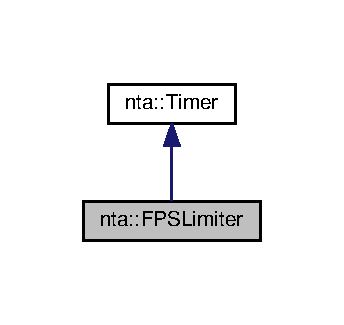
\includegraphics[width=165pt]{de/d03/classnta_1_1FPSLimiter__inherit__graph}
\end{center}
\end{figure}


Collaboration diagram for nta\+:\+:F\+P\+S\+Limiter\+:
\nopagebreak
\begin{figure}[H]
\begin{center}
\leavevmode
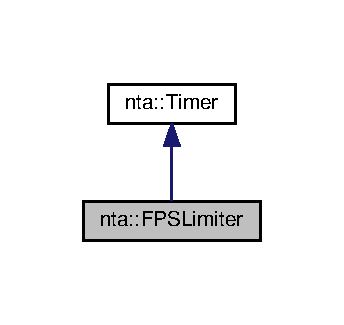
\includegraphics[width=165pt]{de/da2/classnta_1_1FPSLimiter__coll__graph}
\end{center}
\end{figure}
\subsection*{Public Member Functions}
\begin{DoxyCompactItemize}
\item 
\mbox{\Hypertarget{classnta_1_1FPSLimiter_a7a866e0bc883bdd26e80e95748f4052c}\label{classnta_1_1FPSLimiter_a7a866e0bc883bdd26e80e95748f4052c}} 
\hyperlink{classnta_1_1FPSLimiter_a7a866e0bc883bdd26e80e95748f4052c}{F\+P\+S\+Limiter} ()
\begin{DoxyCompactList}\small\item\em constructor and destructor \end{DoxyCompactList}\item 
\mbox{\Hypertarget{classnta_1_1FPSLimiter_ac72ab398095957d9cffa07859e1f97a4}\label{classnta_1_1FPSLimiter_ac72ab398095957d9cffa07859e1f97a4}} 
void \hyperlink{classnta_1_1FPSLimiter_ac72ab398095957d9cffa07859e1f97a4}{set\+Max\+F\+PS} (float max\+F\+PS)
\begin{DoxyCompactList}\small\item\em sets maximum allowed fps \end{DoxyCompactList}\item 
\mbox{\Hypertarget{classnta_1_1FPSLimiter_a682d191b70ddecf8f7ed776dc586fe27}\label{classnta_1_1FPSLimiter_a682d191b70ddecf8f7ed776dc586fe27}} 
float \hyperlink{classnta_1_1FPSLimiter_a682d191b70ddecf8f7ed776dc586fe27}{get\+F\+PS} () const
\begin{DoxyCompactList}\small\item\em gets most recently calculated fps \end{DoxyCompactList}\item 
\mbox{\Hypertarget{classnta_1_1FPSLimiter_a17003ecbc30d60c58112615fcaee4d1e}\label{classnta_1_1FPSLimiter_a17003ecbc30d60c58112615fcaee4d1e}} 
long double \hyperlink{classnta_1_1FPSLimiter_a17003ecbc30d60c58112615fcaee4d1e}{end} ()
\begin{DoxyCompactList}\small\item\em ends fps calculations, delaying if necessary to cap fps \end{DoxyCompactList}\end{DoxyCompactItemize}
\subsection*{Private Attributes}
\begin{DoxyCompactItemize}
\item 
\mbox{\Hypertarget{classnta_1_1FPSLimiter_a06b2818f3bff96da37768829af13df2d}\label{classnta_1_1FPSLimiter_a06b2818f3bff96da37768829af13df2d}} 
float \hyperlink{classnta_1_1FPSLimiter_a06b2818f3bff96da37768829af13df2d}{m\+\_\+fps}
\begin{DoxyCompactList}\small\item\em most recently calculated fps \end{DoxyCompactList}\item 
\mbox{\Hypertarget{classnta_1_1FPSLimiter_ae4a323afb44da70acd962cc4c395183d}\label{classnta_1_1FPSLimiter_ae4a323afb44da70acd962cc4c395183d}} 
float \hyperlink{classnta_1_1FPSLimiter_ae4a323afb44da70acd962cc4c395183d}{m\+\_\+max\+F\+PS}
\begin{DoxyCompactList}\small\item\em maximum allowed fps \end{DoxyCompactList}\end{DoxyCompactItemize}
\subsection*{Additional Inherited Members}


\subsection{Detailed Description}
used to cap the fps of the program at a specific value 

Definition at line 8 of file F\+P\+S\+Limiter.\+h.



The documentation for this class was generated from the following files\+:\begin{DoxyCompactItemize}
\item 
include/nta/F\+P\+S\+Limiter.\+h\item 
src/F\+P\+S\+Limiter.\+cpp\end{DoxyCompactItemize}

\hypertarget{classnta_1_1GetSDLWindowKey}{}\section{nta\+:\+:Get\+S\+D\+L\+Window\+Key Class Reference}
\label{classnta_1_1GetSDLWindowKey}\index{nta\+::\+Get\+S\+D\+L\+Window\+Key@{nta\+::\+Get\+S\+D\+L\+Window\+Key}}


Key for unlocking the Get\+S\+D\+L\+Window() \char`\"{}private\char`\"{} function of class \hyperlink{classnta_1_1Window}{Window}.  




{\ttfamily \#include $<$Window.\+h$>$}

\subsection*{Private Member Functions}
\begin{DoxyCompactItemize}
\item 
\mbox{\Hypertarget{classnta_1_1GetSDLWindowKey_ae963466e80c61d0409855144ad8096e1}\label{classnta_1_1GetSDLWindowKey_ae963466e80c61d0409855144ad8096e1}} 
{\bfseries Get\+S\+D\+L\+Window\+Key} (const \hyperlink{classnta_1_1GetSDLWindowKey}{Get\+S\+D\+L\+Window\+Key} \&)
\item 
\mbox{\Hypertarget{classnta_1_1GetSDLWindowKey_a9753a4f5a30517dce3219a8877fe7cd8}\label{classnta_1_1GetSDLWindowKey_a9753a4f5a30517dce3219a8877fe7cd8}} 
\hyperlink{classnta_1_1GetSDLWindowKey}{Get\+S\+D\+L\+Window\+Key} \& {\bfseries operator=} (const \hyperlink{classnta_1_1GetSDLWindowKey}{Get\+S\+D\+L\+Window\+Key} \&)
\end{DoxyCompactItemize}
\subsection*{Friends}
\begin{DoxyCompactItemize}
\item 
\mbox{\Hypertarget{classnta_1_1GetSDLWindowKey_a888edc649fed896d28811ec69f3f2066}\label{classnta_1_1GetSDLWindowKey_a888edc649fed896d28811ec69f3f2066}} 
class {\bfseries Screen\+Manager}
\end{DoxyCompactItemize}


\subsection{Detailed Description}
Key for unlocking the Get\+S\+D\+L\+Window() \char`\"{}private\char`\"{} function of class \hyperlink{classnta_1_1Window}{Window}. 

Definition at line 14 of file Window.\+h.



The documentation for this class was generated from the following file\+:\begin{DoxyCompactItemize}
\item 
include/nta/Window.\+h\end{DoxyCompactItemize}

\hypertarget{classnta_1_1GLSLProgram}{}\section{nta\+:\+:G\+L\+S\+L\+Program Class Reference}
\label{classnta_1_1GLSLProgram}\index{nta\+::\+G\+L\+S\+L\+Program@{nta\+::\+G\+L\+S\+L\+Program}}


represents a program written in G\+L\+SL comprised of a vertex shader and a fragment shader  




{\ttfamily \#include $<$G\+L\+S\+L\+Program.\+h$>$}

\subsection*{Public Member Functions}
\begin{DoxyCompactItemize}
\item 
\mbox{\Hypertarget{classnta_1_1GLSLProgram_ad8a89f518a3a6ecaa26125d3bbefafaa}\label{classnta_1_1GLSLProgram_ad8a89f518a3a6ecaa26125d3bbefafaa}} 
\hyperlink{classnta_1_1GLSLProgram_ad8a89f518a3a6ecaa26125d3bbefafaa}{G\+L\+S\+L\+Program} ()
\begin{DoxyCompactList}\small\item\em constructor and destructor \end{DoxyCompactList}\item 
\mbox{\Hypertarget{classnta_1_1GLSLProgram_a8140edf8b3d89de4ebf8c4b1db404f59}\label{classnta_1_1GLSLProgram_a8140edf8b3d89de4ebf8c4b1db404f59}} 
G\+Lint \hyperlink{classnta_1_1GLSLProgram_a8140edf8b3d89de4ebf8c4b1db404f59}{get\+Uniform\+Location} (crstring uniform\+Name) const
\begin{DoxyCompactList}\small\item\em returns the location of a uniform in the shaders \end{DoxyCompactList}\item 
\mbox{\Hypertarget{classnta_1_1GLSLProgram_a6067e49c12b542735eff255047cd8ae1}\label{classnta_1_1GLSLProgram_a6067e49c12b542735eff255047cd8ae1}} 
bool \hyperlink{classnta_1_1GLSLProgram_a6067e49c12b542735eff255047cd8ae1}{is\+Linked} () const
\begin{DoxyCompactList}\small\item\em returns whether or not the shaders have been linked \end{DoxyCompactList}\item 
\mbox{\Hypertarget{classnta_1_1GLSLProgram_a708c47abebb9ca01b0eed4d1e711cef7}\label{classnta_1_1GLSLProgram_a708c47abebb9ca01b0eed4d1e711cef7}} 
void \hyperlink{classnta_1_1GLSLProgram_a708c47abebb9ca01b0eed4d1e711cef7}{add\+Attribute} (crstring attribute\+Name)
\begin{DoxyCompactList}\small\item\em makes an attribute useful and assigns it the next available location \end{DoxyCompactList}\item 
\mbox{\Hypertarget{classnta_1_1GLSLProgram_aa1d946246f4b04ba0b947362152ec1c0}\label{classnta_1_1GLSLProgram_aa1d946246f4b04ba0b947362152ec1c0}} 
void \hyperlink{classnta_1_1GLSLProgram_aa1d946246f4b04ba0b947362152ec1c0}{link\+Shaders} ()
\begin{DoxyCompactList}\small\item\em links the compiled shaders to this program \end{DoxyCompactList}\item 
\mbox{\Hypertarget{classnta_1_1GLSLProgram_ac5c8fffb04aec82913b78e35db9ea31f}\label{classnta_1_1GLSLProgram_ac5c8fffb04aec82913b78e35db9ea31f}} 
void \hyperlink{classnta_1_1GLSLProgram_ac5c8fffb04aec82913b78e35db9ea31f}{use} () const
\begin{DoxyCompactList}\small\item\em binds this program \end{DoxyCompactList}\item 
\mbox{\Hypertarget{classnta_1_1GLSLProgram_a3153b4281ab2b6fcf0017c90bbd199af}\label{classnta_1_1GLSLProgram_a3153b4281ab2b6fcf0017c90bbd199af}} 
void \hyperlink{classnta_1_1GLSLProgram_a3153b4281ab2b6fcf0017c90bbd199af}{unuse} () const
\begin{DoxyCompactList}\small\item\em unbinds this program \end{DoxyCompactList}\end{DoxyCompactItemize}
\subsection*{Private Member Functions}
\begin{DoxyCompactItemize}
\item 
\mbox{\Hypertarget{classnta_1_1GLSLProgram_a6de85b6da0514bb9461268ff4806bed5}\label{classnta_1_1GLSLProgram_a6de85b6da0514bb9461268ff4806bed5}} 
void \hyperlink{classnta_1_1GLSLProgram_a6de85b6da0514bb9461268ff4806bed5}{compile\+Shaders} (crstring shader\+Prog\+Name)
\begin{DoxyCompactList}\small\item\em compiles both the vertex and fragment shaders given their name \end{DoxyCompactList}\item 
\mbox{\Hypertarget{classnta_1_1GLSLProgram_a6ec17ca27433ffd2afa0f214fda7eb83}\label{classnta_1_1GLSLProgram_a6ec17ca27433ffd2afa0f214fda7eb83}} 
G\+Luint \hyperlink{classnta_1_1GLSLProgram_a6ec17ca27433ffd2afa0f214fda7eb83}{compile\+Shader} (crstring shader\+File\+Name, G\+Lenum shader\+Type) const
\begin{DoxyCompactList}\small\item\em compiles a shader from a file and returns its id \end{DoxyCompactList}\end{DoxyCompactItemize}
\subsection*{Private Attributes}
\begin{DoxyCompactItemize}
\item 
\mbox{\Hypertarget{classnta_1_1GLSLProgram_ad1019aa2ac0a1cbdef1668870d26c3f2}\label{classnta_1_1GLSLProgram_ad1019aa2ac0a1cbdef1668870d26c3f2}} 
G\+Luint \hyperlink{classnta_1_1GLSLProgram_ad1019aa2ac0a1cbdef1668870d26c3f2}{m\+\_\+program\+ID} = 0
\begin{DoxyCompactList}\small\item\em the id for the program \end{DoxyCompactList}\item 
\mbox{\Hypertarget{classnta_1_1GLSLProgram_a77478858f3885fba34a384ace272565a}\label{classnta_1_1GLSLProgram_a77478858f3885fba34a384ace272565a}} 
G\+Luint \hyperlink{classnta_1_1GLSLProgram_a77478858f3885fba34a384ace272565a}{m\+\_\+vert\+Shader\+ID} = 0
\begin{DoxyCompactList}\small\item\em the ids for the vertex and fragment shaders \end{DoxyCompactList}\item 
\mbox{\Hypertarget{classnta_1_1GLSLProgram_a4762bd58f72875cdda7513684f530bed}\label{classnta_1_1GLSLProgram_a4762bd58f72875cdda7513684f530bed}} 
G\+Luint {\bfseries m\+\_\+frag\+Shader\+ID} = 0
\item 
\mbox{\Hypertarget{classnta_1_1GLSLProgram_aa90cbc60f99bdfc69ef68633e351a118}\label{classnta_1_1GLSLProgram_aa90cbc60f99bdfc69ef68633e351a118}} 
int \hyperlink{classnta_1_1GLSLProgram_aa90cbc60f99bdfc69ef68633e351a118}{m\+\_\+num\+Attributes} = 0
\begin{DoxyCompactList}\small\item\em the number of attributes used by the vertex shader \end{DoxyCompactList}\item 
\mbox{\Hypertarget{classnta_1_1GLSLProgram_af133a0d5d2e15fdff99062f9ea742024}\label{classnta_1_1GLSLProgram_af133a0d5d2e15fdff99062f9ea742024}} 
bool \hyperlink{classnta_1_1GLSLProgram_af133a0d5d2e15fdff99062f9ea742024}{m\+\_\+is\+Linked} = false
\begin{DoxyCompactList}\small\item\em keeps track of whether or not the shaders have been linked \end{DoxyCompactList}\end{DoxyCompactItemize}
\subsection*{Friends}
\begin{DoxyCompactItemize}
\item 
\mbox{\Hypertarget{classnta_1_1GLSLProgram_ab1ef2aa9992dd8ae85793e1a1f980e1e}\label{classnta_1_1GLSLProgram_ab1ef2aa9992dd8ae85793e1a1f980e1e}} 
class {\bfseries System\+Manager}
\end{DoxyCompactItemize}


\subsection{Detailed Description}
represents a program written in G\+L\+SL comprised of a vertex shader and a fragment shader 

Definition at line 13 of file G\+L\+S\+L\+Program.\+h.



The documentation for this class was generated from the following files\+:\begin{DoxyCompactItemize}
\item 
include/nta/G\+L\+S\+L\+Program.\+h\item 
src/G\+L\+S\+L\+Program.\+cpp\end{DoxyCompactItemize}

\hypertarget{structnta_1_1GLTexture}{}\section{nta\+:\+:G\+L\+Texture Struct Reference}
\label{structnta_1_1GLTexture}\index{nta\+::\+G\+L\+Texture@{nta\+::\+G\+L\+Texture}}


represents a texture  




{\ttfamily \#include $<$G\+L\+Texture.\+h$>$}

\subsection*{Public Member Functions}
\begin{DoxyCompactItemize}
\item 
\mbox{\Hypertarget{structnta_1_1GLTexture_a85233cfdf7788bc8461435482caf01d9}\label{structnta_1_1GLTexture_a85233cfdf7788bc8461435482caf01d9}} 
bool {\bfseries is\+\_\+valid} () const
\end{DoxyCompactItemize}
\subsection*{Static Public Member Functions}
\begin{DoxyCompactItemize}
\item 
\mbox{\Hypertarget{structnta_1_1GLTexture_abc80887334f8020512952c6093e99f14}\label{structnta_1_1GLTexture_abc80887334f8020512952c6093e99f14}} 
static \hyperlink{structnta_1_1GLTexture}{G\+L\+Texture} {\bfseries no\+\_\+texture} ()
\end{DoxyCompactItemize}
\subsection*{Public Attributes}
\begin{DoxyCompactItemize}
\item 
\mbox{\Hypertarget{structnta_1_1GLTexture_aaf0d536088f4b1062d996679b217c0f9}\label{structnta_1_1GLTexture_aaf0d536088f4b1062d996679b217c0f9}} 
G\+Luint \hyperlink{structnta_1_1GLTexture_aaf0d536088f4b1062d996679b217c0f9}{id}
\begin{DoxyCompactList}\small\item\em the id of the texture \end{DoxyCompactList}\item 
\mbox{\Hypertarget{structnta_1_1GLTexture_a8f4d13ab2b19b700f76334c46458ac48}\label{structnta_1_1GLTexture_a8f4d13ab2b19b700f76334c46458ac48}} 
G\+Lint \hyperlink{structnta_1_1GLTexture_a8f4d13ab2b19b700f76334c46458ac48}{width}
\begin{DoxyCompactList}\small\item\em the width and height, respectively, of the texture \end{DoxyCompactList}\item 
\mbox{\Hypertarget{structnta_1_1GLTexture_a4ac2e45733ffb16238eb696d663e62a1}\label{structnta_1_1GLTexture_a4ac2e45733ffb16238eb696d663e62a1}} 
G\+Lint {\bfseries height}
\end{DoxyCompactItemize}


\subsection{Detailed Description}
represents a texture 

Definition at line 11 of file G\+L\+Texture.\+h.



Collaboration diagram for nta\+:\+:G\+L\+Texture\+:\nopagebreak
\begin{figure}[H]
\begin{center}
\leavevmode
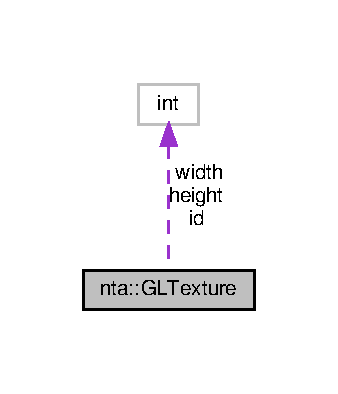
\includegraphics[width=162pt]{d3/d3e/structnta_1_1GLTexture__coll__graph}
\end{center}
\end{figure}


The documentation for this struct was generated from the following file\+:\begin{DoxyCompactItemize}
\item 
include/nta/G\+L\+Texture.\+h\end{DoxyCompactItemize}

\hypertarget{structnta_1_1Glyph}{}\section{nta\+:\+:Glyph Struct Reference}
\label{structnta_1_1Glyph}\index{nta\+::\+Glyph@{nta\+::\+Glyph}}


represents what is essentially a sprite  




{\ttfamily \#include $<$Sprite\+Batch.\+h$>$}



Collaboration diagram for nta\+:\+:Glyph\+:
\nopagebreak
\begin{figure}[H]
\begin{center}
\leavevmode
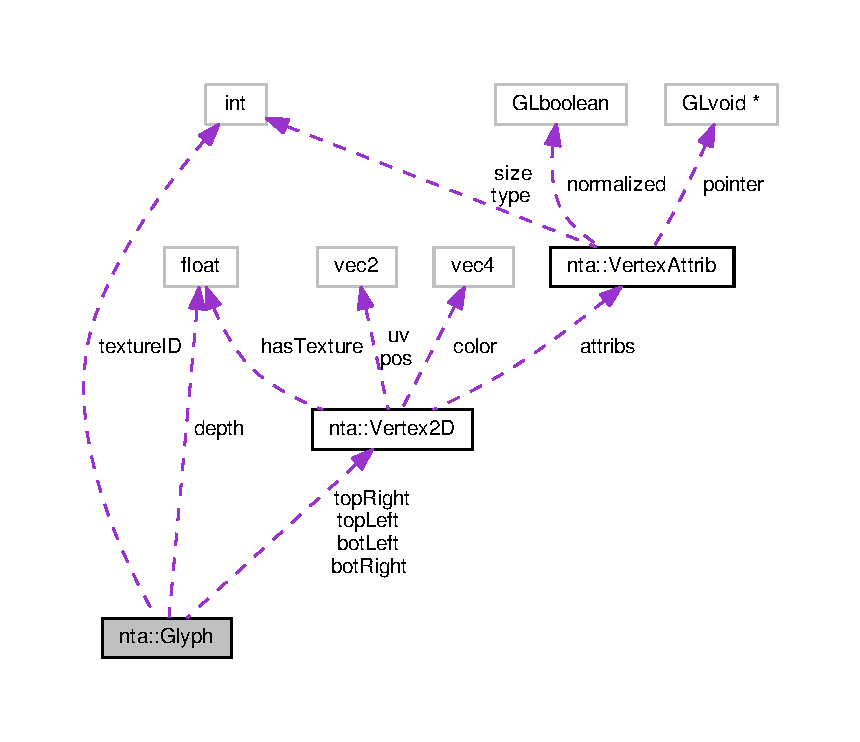
\includegraphics[width=159pt]{d8/d54/structnta_1_1Glyph__coll__graph}
\end{center}
\end{figure}
\subsection*{Public Member Functions}
\begin{DoxyCompactItemize}
\item 
\mbox{\Hypertarget{structnta_1_1Glyph_ae400ec6b413eee3d1f091ff9cc594bba}\label{structnta_1_1Glyph_ae400ec6b413eee3d1f091ff9cc594bba}} 
{\bfseries Glyph} (crvec4 pos\+Rect, crvec4 uv\+Rect, G\+Luint texture, float d, crvec4 color)
\end{DoxyCompactItemize}
\subsection*{Public Attributes}
\begin{DoxyCompactItemize}
\item 
\mbox{\Hypertarget{structnta_1_1Glyph_acd8af1fcb19c4fb960808defbee5abe5}\label{structnta_1_1Glyph_acd8af1fcb19c4fb960808defbee5abe5}} 
G\+Luint \hyperlink{structnta_1_1Glyph_acd8af1fcb19c4fb960808defbee5abe5}{texture\+ID}
\begin{DoxyCompactList}\small\item\em the texture used by the glyph \end{DoxyCompactList}\item 
\mbox{\Hypertarget{structnta_1_1Glyph_a259a2061c71dfd9fa0857f52d4daff8a}\label{structnta_1_1Glyph_a259a2061c71dfd9fa0857f52d4daff8a}} 
float \hyperlink{structnta_1_1Glyph_a259a2061c71dfd9fa0857f52d4daff8a}{depth}
\begin{DoxyCompactList}\small\item\em the depth of the glyph \end{DoxyCompactList}\item 
\mbox{\Hypertarget{structnta_1_1Glyph_a71969ecd8d228e48f9dff95787187282}\label{structnta_1_1Glyph_a71969ecd8d228e48f9dff95787187282}} 
\hyperlink{structnta_1_1Vertex2D}{Vertex2D} \hyperlink{structnta_1_1Glyph_a71969ecd8d228e48f9dff95787187282}{top\+Left}
\begin{DoxyCompactList}\small\item\em the vertices of the four corners of the glyph \end{DoxyCompactList}\item 
\mbox{\Hypertarget{structnta_1_1Glyph_a50ce474e9d7b6088e88d991d16f4b047}\label{structnta_1_1Glyph_a50ce474e9d7b6088e88d991d16f4b047}} 
\hyperlink{structnta_1_1Vertex2D}{Vertex2D} {\bfseries top\+Right}
\item 
\mbox{\Hypertarget{structnta_1_1Glyph_a5d911b010ab2b67cd4c9e642faf3cbf2}\label{structnta_1_1Glyph_a5d911b010ab2b67cd4c9e642faf3cbf2}} 
\hyperlink{structnta_1_1Vertex2D}{Vertex2D} {\bfseries bot\+Right}
\item 
\mbox{\Hypertarget{structnta_1_1Glyph_aba92c1f9cb4d5e17270d90a4f5d19b0b}\label{structnta_1_1Glyph_aba92c1f9cb4d5e17270d90a4f5d19b0b}} 
\hyperlink{structnta_1_1Vertex2D}{Vertex2D} {\bfseries bot\+Left}
\end{DoxyCompactItemize}


\subsection{Detailed Description}
represents what is essentially a sprite 

Definition at line 13 of file Sprite\+Batch.\+h.



The documentation for this struct was generated from the following file\+:\begin{DoxyCompactItemize}
\item 
include/nta/Sprite\+Batch.\+h\end{DoxyCompactItemize}

\hypertarget{classnta_1_1HuffmanLeaf}{}\section{nta\+:\+:Huffman\+Leaf Class Reference}
\label{classnta_1_1HuffmanLeaf}\index{nta\+::\+Huffman\+Leaf@{nta\+::\+Huffman\+Leaf}}


represents a leaf in a Huffman tree  




{\ttfamily \#include $<$Compressor.\+h$>$}



Inheritance diagram for nta\+:\+:Huffman\+Leaf\+:\nopagebreak
\begin{figure}[H]
\begin{center}
\leavevmode
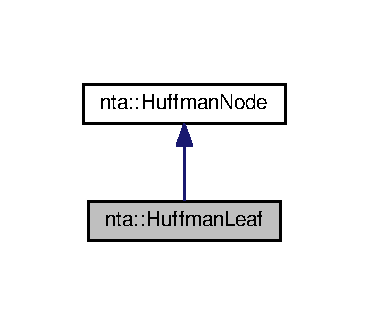
\includegraphics[width=177pt]{df/d39/classnta_1_1HuffmanLeaf__inherit__graph}
\end{center}
\end{figure}


Collaboration diagram for nta\+:\+:Huffman\+Leaf\+:\nopagebreak
\begin{figure}[H]
\begin{center}
\leavevmode
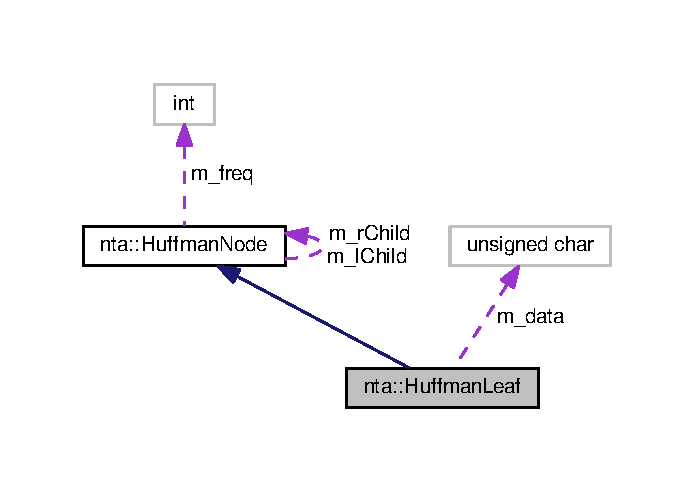
\includegraphics[width=238pt]{d7/d69/classnta_1_1HuffmanLeaf__coll__graph}
\end{center}
\end{figure}
\subsection*{Public Member Functions}
\begin{DoxyCompactItemize}
\item 
\mbox{\Hypertarget{classnta_1_1HuffmanLeaf_afcd113b293d90d3297d409421bbfb285}\label{classnta_1_1HuffmanLeaf_afcd113b293d90d3297d409421bbfb285}} 
\hyperlink{classnta_1_1HuffmanLeaf_afcd113b293d90d3297d409421bbfb285}{Huffman\+Leaf} ()
\begin{DoxyCompactList}\small\item\em basic constructor \end{DoxyCompactList}\item 
\mbox{\Hypertarget{classnta_1_1HuffmanLeaf_a68e98537fe635d83cc04a2ce70e99993}\label{classnta_1_1HuffmanLeaf_a68e98537fe635d83cc04a2ce70e99993}} 
\hyperlink{classnta_1_1HuffmanLeaf_a68e98537fe635d83cc04a2ce70e99993}{Huffman\+Leaf} (G\+Lubyte data, int freq)
\begin{DoxyCompactList}\small\item\em constructs a leaf with given data and freq \end{DoxyCompactList}\item 
\mbox{\Hypertarget{classnta_1_1HuffmanLeaf_a579b5b814ae18f2230a07c186f96890f}\label{classnta_1_1HuffmanLeaf_a579b5b814ae18f2230a07c186f96890f}} 
\hyperlink{classnta_1_1HuffmanLeaf_a579b5b814ae18f2230a07c186f96890f}{$\sim$\+Huffman\+Leaf} ()
\begin{DoxyCompactList}\small\item\em destroys leaf \end{DoxyCompactList}\item 
\mbox{\Hypertarget{classnta_1_1HuffmanLeaf_aebdea9a65041b1bca7dc89a32a44d0f3}\label{classnta_1_1HuffmanLeaf_aebdea9a65041b1bca7dc89a32a44d0f3}} 
G\+Lubyte \hyperlink{classnta_1_1HuffmanLeaf_aebdea9a65041b1bca7dc89a32a44d0f3}{get\+Data} () const
\begin{DoxyCompactList}\small\item\em returns m\+\_\+data \end{DoxyCompactList}\end{DoxyCompactItemize}
\subsection*{Private Attributes}
\begin{DoxyCompactItemize}
\item 
\mbox{\Hypertarget{classnta_1_1HuffmanLeaf_a1a02d12c1ee80e4d3686fb05a0d140b0}\label{classnta_1_1HuffmanLeaf_a1a02d12c1ee80e4d3686fb05a0d140b0}} 
G\+Lubyte \hyperlink{classnta_1_1HuffmanLeaf_a1a02d12c1ee80e4d3686fb05a0d140b0}{m\+\_\+data}
\begin{DoxyCompactList}\small\item\em the byte associated with the leaf \end{DoxyCompactList}\end{DoxyCompactItemize}
\subsection*{Additional Inherited Members}


\subsection{Detailed Description}
represents a leaf in a Huffman tree 

Definition at line 38 of file Compressor.\+h.



The documentation for this class was generated from the following files\+:\begin{DoxyCompactItemize}
\item 
include/nta/Compressor.\+h\item 
src/Huffman\+Leaf.\+cpp\end{DoxyCompactItemize}

\hypertarget{classnta_1_1HuffmanNode}{}\section{nta\+:\+:Huffman\+Node Class Reference}
\label{classnta_1_1HuffmanNode}\index{nta\+::\+Huffman\+Node@{nta\+::\+Huffman\+Node}}


A node in a Huffman tree.  




{\ttfamily \#include $<$Compressor.\+h$>$}



Inheritance diagram for nta\+:\+:Huffman\+Node\+:\nopagebreak
\begin{figure}[H]
\begin{center}
\leavevmode
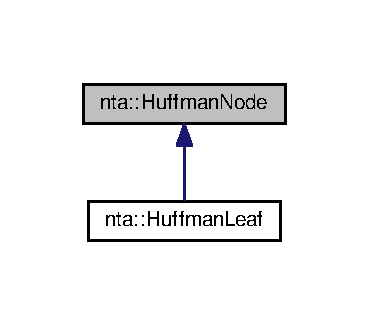
\includegraphics[width=177pt]{d4/d0d/classnta_1_1HuffmanNode__inherit__graph}
\end{center}
\end{figure}


Collaboration diagram for nta\+:\+:Huffman\+Node\+:\nopagebreak
\begin{figure}[H]
\begin{center}
\leavevmode
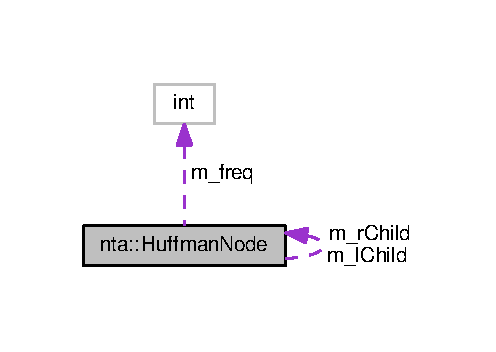
\includegraphics[width=238pt]{d5/d0a/classnta_1_1HuffmanNode__coll__graph}
\end{center}
\end{figure}
\subsection*{Public Member Functions}
\begin{DoxyCompactItemize}
\item 
\mbox{\Hypertarget{classnta_1_1HuffmanNode_a6e92a7ee38fd56994c2eb2d894d3d108}\label{classnta_1_1HuffmanNode_a6e92a7ee38fd56994c2eb2d894d3d108}} 
\hyperlink{classnta_1_1HuffmanNode_a6e92a7ee38fd56994c2eb2d894d3d108}{Huffman\+Node} ()
\begin{DoxyCompactList}\small\item\em basic constructor \end{DoxyCompactList}\item 
\mbox{\Hypertarget{classnta_1_1HuffmanNode_ae9aa27c2ed1cd215e3fe6a5fc48a0527}\label{classnta_1_1HuffmanNode_ae9aa27c2ed1cd215e3fe6a5fc48a0527}} 
\hyperlink{classnta_1_1HuffmanNode_ae9aa27c2ed1cd215e3fe6a5fc48a0527}{Huffman\+Node} (\hyperlink{classnta_1_1HuffmanNode}{Huffman\+Node} $\ast$l, \hyperlink{classnta_1_1HuffmanNode}{Huffman\+Node} $\ast$r)
\begin{DoxyCompactList}\small\item\em sets l and r as children of this and sets m\+\_\+freq to the sum of their frequencies \end{DoxyCompactList}\item 
\mbox{\Hypertarget{classnta_1_1HuffmanNode_a45afade3ee4a50baba8daa66edd32e72}\label{classnta_1_1HuffmanNode_a45afade3ee4a50baba8daa66edd32e72}} 
virtual \hyperlink{classnta_1_1HuffmanNode_a45afade3ee4a50baba8daa66edd32e72}{$\sim$\+Huffman\+Node} ()
\begin{DoxyCompactList}\small\item\em recursively destroys node \end{DoxyCompactList}\item 
\mbox{\Hypertarget{classnta_1_1HuffmanNode_abbdee24e11a5a72a54f6187228f9b7f0}\label{classnta_1_1HuffmanNode_abbdee24e11a5a72a54f6187228f9b7f0}} 
auto \hyperlink{classnta_1_1HuffmanNode_abbdee24e11a5a72a54f6187228f9b7f0}{get\+Encodings} (crstring enc=\char`\"{}\char`\"{}) const -\/$>$ std\+::map$<$ G\+Lubyte, std\+::string $>$
\begin{DoxyCompactList}\small\item\em returns map of all the bytes and how they are encoded \end{DoxyCompactList}\item 
\mbox{\Hypertarget{classnta_1_1HuffmanNode_a2f67fd062ac5079cd40a0a82352d5a45}\label{classnta_1_1HuffmanNode_a2f67fd062ac5079cd40a0a82352d5a45}} 
\hyperlink{classnta_1_1HuffmanNode}{Huffman\+Node} $\ast$ \hyperlink{classnta_1_1HuffmanNode_a2f67fd062ac5079cd40a0a82352d5a45}{get\+Left} () const
\begin{DoxyCompactList}\small\item\em returns children \end{DoxyCompactList}\item 
\mbox{\Hypertarget{classnta_1_1HuffmanNode_a3be8400f944090f38c48b17e890e5105}\label{classnta_1_1HuffmanNode_a3be8400f944090f38c48b17e890e5105}} 
\hyperlink{classnta_1_1HuffmanNode}{Huffman\+Node} $\ast$ {\bfseries get\+Right} () const
\item 
\mbox{\Hypertarget{classnta_1_1HuffmanNode_a429374a0e433063935f6e86816be8831}\label{classnta_1_1HuffmanNode_a429374a0e433063935f6e86816be8831}} 
bool \hyperlink{classnta_1_1HuffmanNode_a429374a0e433063935f6e86816be8831}{has\+Children} () const
\begin{DoxyCompactList}\small\item\em returns whether or not the node has children \end{DoxyCompactList}\item 
\mbox{\Hypertarget{classnta_1_1HuffmanNode_aaae7f78797726f30ce584e6fd0a282c1}\label{classnta_1_1HuffmanNode_aaae7f78797726f30ce584e6fd0a282c1}} 
int \hyperlink{classnta_1_1HuffmanNode_aaae7f78797726f30ce584e6fd0a282c1}{get\+Frequency} () const
\begin{DoxyCompactList}\small\item\em returns the frequency of the node \end{DoxyCompactList}\end{DoxyCompactItemize}
\subsection*{Protected Attributes}
\begin{DoxyCompactItemize}
\item 
\mbox{\Hypertarget{classnta_1_1HuffmanNode_acba67dc4c5cda81fa4f761a314b57d86}\label{classnta_1_1HuffmanNode_acba67dc4c5cda81fa4f761a314b57d86}} 
int \hyperlink{classnta_1_1HuffmanNode_acba67dc4c5cda81fa4f761a314b57d86}{m\+\_\+freq}
\begin{DoxyCompactList}\small\item\em the frequency of the nodes associated bytes \end{DoxyCompactList}\end{DoxyCompactItemize}
\subsection*{Private Attributes}
\begin{DoxyCompactItemize}
\item 
\mbox{\Hypertarget{classnta_1_1HuffmanNode_ae8cdbf035355dfbe64bdba9b2b29a589}\label{classnta_1_1HuffmanNode_ae8cdbf035355dfbe64bdba9b2b29a589}} 
\hyperlink{classnta_1_1HuffmanNode}{Huffman\+Node} $\ast$ \hyperlink{classnta_1_1HuffmanNode_ae8cdbf035355dfbe64bdba9b2b29a589}{m\+\_\+l\+Child}
\begin{DoxyCompactList}\small\item\em the children of the node \end{DoxyCompactList}\item 
\mbox{\Hypertarget{classnta_1_1HuffmanNode_adfc2e8ad6db0b3a46d7187a7c839d350}\label{classnta_1_1HuffmanNode_adfc2e8ad6db0b3a46d7187a7c839d350}} 
\hyperlink{classnta_1_1HuffmanNode}{Huffman\+Node} $\ast$ {\bfseries m\+\_\+r\+Child}
\end{DoxyCompactItemize}


\subsection{Detailed Description}
A node in a Huffman tree. 

Definition at line 13 of file Compressor.\+h.



The documentation for this class was generated from the following files\+:\begin{DoxyCompactItemize}
\item 
include/nta/Compressor.\+h\item 
src/Huffman\+Node.\+cpp\end{DoxyCompactItemize}

\hypertarget{classnta_1_1ImageLoader}{}\section{nta\+:\+:Image\+Loader Class Reference}
\label{classnta_1_1ImageLoader}\index{nta\+::\+Image\+Loader@{nta\+::\+Image\+Loader}}


loads images as G\+L\+Textures  




{\ttfamily \#include $<$G\+L\+Texture.\+h$>$}

\subsection*{Static Private Member Functions}
\begin{DoxyCompactItemize}
\item 
\mbox{\Hypertarget{classnta_1_1ImageLoader_a9144fea6007e8dc1af75ee4da5a02f10}\label{classnta_1_1ImageLoader_a9144fea6007e8dc1af75ee4da5a02f10}} 
static \hyperlink{namespacenta_d3/dff/structnta_1_1GLTexture}{G\+L\+Texture} \hyperlink{classnta_1_1ImageLoader_a9144fea6007e8dc1af75ee4da5a02f10}{read\+Image} (crstring file\+Path, G\+Lint min\+Filt, G\+Lint mag\+Filt, crvec2 dimensions)
\begin{DoxyCompactList}\small\item\em loads in any image file \end{DoxyCompactList}\end{DoxyCompactItemize}
\subsection*{Friends}
\begin{DoxyCompactItemize}
\item 
\mbox{\Hypertarget{classnta_1_1ImageLoader_a54c1252abc87a78a301e6b6984470408}\label{classnta_1_1ImageLoader_a54c1252abc87a78a301e6b6984470408}} 
class {\bfseries Resource\+Manager}
\end{DoxyCompactItemize}


\subsection{Detailed Description}
loads images as G\+L\+Textures 

Definition at line 18 of file G\+L\+Texture.\+h.



The documentation for this class was generated from the following files\+:\begin{DoxyCompactItemize}
\item 
include/nta/G\+L\+Texture.\+h\item 
src/G\+L\+Texture.\+cpp\end{DoxyCompactItemize}

\hypertarget{classnta_1_1InputManager}{}\section{nta\+:\+:Input\+Manager Class Reference}
\label{classnta_1_1InputManager}\index{nta\+::\+Input\+Manager@{nta\+::\+Input\+Manager}}


keeps track of all input  




{\ttfamily \#include $<$Input\+Manager.\+h$>$}

\subsection*{Static Public Member Functions}
\begin{DoxyCompactItemize}
\item 
\mbox{\Hypertarget{classnta_1_1InputManager_abaa04adc67f8025133fd1360b171b95f}\label{classnta_1_1InputManager_abaa04adc67f8025133fd1360b171b95f}} 
static glm\+::vec2 \hyperlink{classnta_1_1InputManager_abaa04adc67f8025133fd1360b171b95f}{get\+Mouse\+Coords} ()
\begin{DoxyCompactList}\small\item\em returns the mouse\textquotesingle{}s coordinates \end{DoxyCompactList}\item 
\mbox{\Hypertarget{classnta_1_1InputManager_a899371ac784e0a1aeb6f9dc1e7f0f58c}\label{classnta_1_1InputManager_a899371ac784e0a1aeb6f9dc1e7f0f58c}} 
static glm\+::vec2 \hyperlink{classnta_1_1InputManager_a899371ac784e0a1aeb6f9dc1e7f0f58c}{get\+Mouse\+Coords\+Standard} (int height)
\begin{DoxyCompactList}\small\item\em returns the mouse\textquotesingle{}s coordinates with the y axis flipped (0 represents the bottom of the screen instead of top) \end{DoxyCompactList}\item 
\mbox{\Hypertarget{classnta_1_1InputManager_a9f308e79f224806eb923ce2ef0f8023a}\label{classnta_1_1InputManager_a9f308e79f224806eb923ce2ef0f8023a}} 
static \hyperlink{namespacenta_aabafd53ba7264997db9e6e934a8ade2b}{Mouse\+Wheel\+Motion} \hyperlink{classnta_1_1InputManager_a9f308e79f224806eb923ce2ef0f8023a}{get\+Mouse\+Wheel\+Motion} ()
\begin{DoxyCompactList}\small\item\em returns the mouse wheel\textquotesingle{}s motion \end{DoxyCompactList}\item 
\mbox{\Hypertarget{classnta_1_1InputManager_ae97dfcf9043a3590a02387af85669871}\label{classnta_1_1InputManager_ae97dfcf9043a3590a02387af85669871}} 
static bool \hyperlink{classnta_1_1InputManager_ae97dfcf9043a3590a02387af85669871}{is\+Pressed} (unsigned int key)
\begin{DoxyCompactList}\small\item\em returns whether or not specified key is pressed \end{DoxyCompactList}\item 
\mbox{\Hypertarget{classnta_1_1InputManager_a63f1bc4d75790755fa260f273546630d}\label{classnta_1_1InputManager_a63f1bc4d75790755fa260f273546630d}} 
static bool \hyperlink{classnta_1_1InputManager_a63f1bc4d75790755fa260f273546630d}{just\+Pressed} (unsigned int key)
\begin{DoxyCompactList}\small\item\em returns whether or not the key was just pressed this frame \end{DoxyCompactList}\item 
\mbox{\Hypertarget{classnta_1_1InputManager_a2e4b4450234805eca3837bc8d365d0bc}\label{classnta_1_1InputManager_a2e4b4450234805eca3837bc8d365d0bc}} 
static bool \hyperlink{classnta_1_1InputManager_a2e4b4450234805eca3837bc8d365d0bc}{just\+Released} (unsigned int key)
\begin{DoxyCompactList}\small\item\em returns whether or not the key was just released this frame \end{DoxyCompactList}\item 
\mbox{\Hypertarget{classnta_1_1InputManager_a190e5a8e2c26f28648538be7b4bea9e0}\label{classnta_1_1InputManager_a190e5a8e2c26f28648538be7b4bea9e0}} 
static void \hyperlink{classnta_1_1InputManager_a190e5a8e2c26f28648538be7b4bea9e0}{press\+Key} (unsigned int key)
\begin{DoxyCompactList}\small\item\em tells \hyperlink{classnta_1_1InputManager}{Input\+Manager} that specified key was pressed \end{DoxyCompactList}\item 
\mbox{\Hypertarget{classnta_1_1InputManager_acb2f11b5580141d4c3345499eea485c0}\label{classnta_1_1InputManager_acb2f11b5580141d4c3345499eea485c0}} 
static void \hyperlink{classnta_1_1InputManager_acb2f11b5580141d4c3345499eea485c0}{release\+Key} (unsigned int key)
\begin{DoxyCompactList}\small\item\em tells \hyperlink{classnta_1_1InputManager}{Input\+Manager} that specified key was released \end{DoxyCompactList}\item 
\mbox{\Hypertarget{classnta_1_1InputManager_a42590ba480b5fd5280cbc69732bb025f}\label{classnta_1_1InputManager_a42590ba480b5fd5280cbc69732bb025f}} 
static void \hyperlink{classnta_1_1InputManager_a42590ba480b5fd5280cbc69732bb025f}{set\+Mouse\+Coords} (float x, float y)
\begin{DoxyCompactList}\small\item\em tells \hyperlink{classnta_1_1InputManager}{Input\+Manager} where the mouse is \end{DoxyCompactList}\item 
\mbox{\Hypertarget{classnta_1_1InputManager_a716c722f10dfe636b79384087bbf1a6e}\label{classnta_1_1InputManager_a716c722f10dfe636b79384087bbf1a6e}} 
static void \hyperlink{classnta_1_1InputManager_a716c722f10dfe636b79384087bbf1a6e}{set\+Mouse\+Wheel\+Motion} (const \hyperlink{namespacenta_aabafd53ba7264997db9e6e934a8ade2b}{Mouse\+Wheel\+Motion} \&motion)
\begin{DoxyCompactList}\small\item\em tells \hyperlink{classnta_1_1InputManager}{Input\+Manager} how the wheel is rolling \end{DoxyCompactList}\item 
\mbox{\Hypertarget{classnta_1_1InputManager_a7c555e0a2ce37af042b5016140414f18}\label{classnta_1_1InputManager_a7c555e0a2ce37af042b5016140414f18}} 
static void \hyperlink{classnta_1_1InputManager_a7c555e0a2ce37af042b5016140414f18}{update} (S\+D\+L\+\_\+\+Event \&event)
\begin{DoxyCompactList}\small\item\em updates the state of m\+\_\+\+Key\+Map \end{DoxyCompactList}\item 
\mbox{\Hypertarget{classnta_1_1InputManager_aea4219a830a2b1d9ee87bdc5f954903d}\label{classnta_1_1InputManager_aea4219a830a2b1d9ee87bdc5f954903d}} 
static void \hyperlink{classnta_1_1InputManager_aea4219a830a2b1d9ee87bdc5f954903d}{update\+Prev} ()
\begin{DoxyCompactList}\small\item\em updates the state of m\+\_\+prev\+Key\+Map \end{DoxyCompactList}\end{DoxyCompactItemize}
\subsection*{Static Private Attributes}
\begin{DoxyCompactItemize}
\item 
\mbox{\Hypertarget{classnta_1_1InputManager_a00aa67b739a6762219dc97cc2e23c3f5}\label{classnta_1_1InputManager_a00aa67b739a6762219dc97cc2e23c3f5}} 
static std\+::unordered\+\_\+map$<$ unsigned int, bool $>$ \hyperlink{classnta_1_1InputManager_a00aa67b739a6762219dc97cc2e23c3f5}{m\+\_\+key\+Map}
\begin{DoxyCompactList}\small\item\em stores whether each key is pressed or not \end{DoxyCompactList}\item 
\mbox{\Hypertarget{classnta_1_1InputManager_a5fef83321ad801f59f5a4f3b2542db47}\label{classnta_1_1InputManager_a5fef83321ad801f59f5a4f3b2542db47}} 
static std\+::unordered\+\_\+map$<$ unsigned int, bool $>$ \hyperlink{classnta_1_1InputManager_a5fef83321ad801f59f5a4f3b2542db47}{m\+\_\+prev\+Key\+Map}
\begin{DoxyCompactList}\small\item\em stores whether the key was pressed last frame or not \end{DoxyCompactList}\item 
\mbox{\Hypertarget{classnta_1_1InputManager_a9f0b4d6c78182a49313144c712cb460e}\label{classnta_1_1InputManager_a9f0b4d6c78182a49313144c712cb460e}} 
static glm\+::vec2 \hyperlink{classnta_1_1InputManager_a9f0b4d6c78182a49313144c712cb460e}{m\+\_\+mouse\+Coords}
\begin{DoxyCompactList}\small\item\em stores the location of the mouse in mouse coordinates \end{DoxyCompactList}\item 
\mbox{\Hypertarget{classnta_1_1InputManager_ae66e8c723d33a51ece6700e266191f01}\label{classnta_1_1InputManager_ae66e8c723d33a51ece6700e266191f01}} 
static \hyperlink{namespacenta_aabafd53ba7264997db9e6e934a8ade2b}{Mouse\+Wheel\+Motion} \hyperlink{classnta_1_1InputManager_ae66e8c723d33a51ece6700e266191f01}{m\+\_\+mouse\+Wheel\+Motion}
\begin{DoxyCompactList}\small\item\em stores the motion of the mouse wheel \end{DoxyCompactList}\end{DoxyCompactItemize}


\subsection{Detailed Description}
keeps track of all input 

Definition at line 12 of file Input\+Manager.\+h.



Collaboration diagram for nta\+:\+:Input\+Manager\+:\nopagebreak
\begin{figure}[H]
\begin{center}
\leavevmode
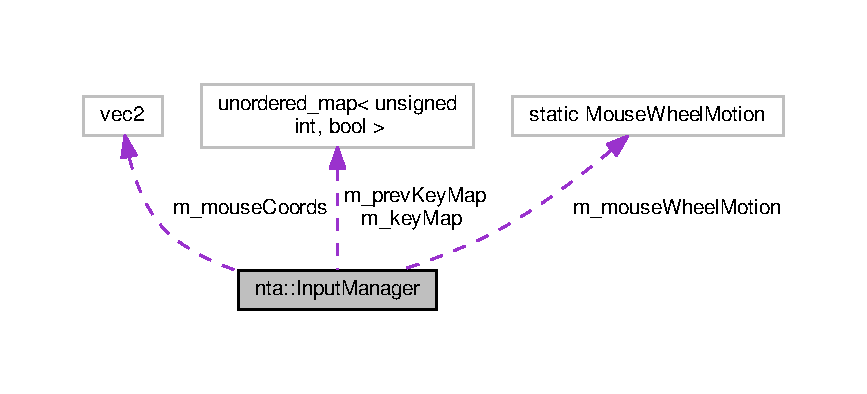
\includegraphics[width=350pt]{dc/d97/classnta_1_1InputManager__coll__graph}
\end{center}
\end{figure}


The documentation for this class was generated from the following files\+:\begin{DoxyCompactItemize}
\item 
include/nta/Input\+Manager.\+h\item 
src/Input\+Manager.\+cpp\end{DoxyCompactItemize}

\hypertarget{classnta_1_1IOManager}{}\section{nta\+:\+:I\+O\+Manager Class Reference}
\label{classnta_1_1IOManager}\index{nta\+::\+I\+O\+Manager@{nta\+::\+I\+O\+Manager}}


Handles binary file operations.  




{\ttfamily \#include $<$I\+O\+Manager.\+h$>$}

\subsection*{Static Public Member Functions}
\begin{DoxyCompactItemize}
\item 
\mbox{\Hypertarget{classnta_1_1IOManager_a8225f73838465f27e6fa60b689496d10}\label{classnta_1_1IOManager_a8225f73838465f27e6fa60b689496d10}} 
static void \hyperlink{classnta_1_1IOManager_a8225f73838465f27e6fa60b689496d10}{read\+File\+To\+Buffer} (crstring file\+Path, File\+Buffer \&buffer)
\begin{DoxyCompactList}\small\item\em stores the entire contents of a file in a buffer \end{DoxyCompactList}\item 
static void \hyperlink{classnta_1_1IOManager_abbfd9da05b22aa488043a19344d38e0a}{read\+File\+To\+Buffer} (crstring file\+Path, std\+::string \&buffer)
\item 
\mbox{\Hypertarget{classnta_1_1IOManager_a8e22ef5a2e46a48abdefa21847cf9eff}\label{classnta_1_1IOManager_a8e22ef5a2e46a48abdefa21847cf9eff}} 
static void \hyperlink{classnta_1_1IOManager_a8e22ef5a2e46a48abdefa21847cf9eff}{write\+File\+From\+Buffer} (crstring file\+Path, const File\+Buffer \&buffer)
\begin{DoxyCompactList}\small\item\em stores the entire contents of a buffer in a file \end{DoxyCompactList}\item 
\mbox{\Hypertarget{classnta_1_1IOManager_a88a69469ca9a8c4a632e7d7e14ae3d79}\label{classnta_1_1IOManager_a88a69469ca9a8c4a632e7d7e14ae3d79}} 
static void {\bfseries write\+File\+From\+Buffer} (crstring file\+Path, crstring buffer)
\item 
\mbox{\Hypertarget{classnta_1_1IOManager_aa9855baef3ed91e4e95e3a5e899ba473}\label{classnta_1_1IOManager_aa9855baef3ed91e4e95e3a5e899ba473}} 
static void \hyperlink{classnta_1_1IOManager_aa9855baef3ed91e4e95e3a5e899ba473}{write\+Float\+LE} (float val, std\+::ofstream \&file)
\begin{DoxyCompactList}\small\item\em writes/reads a float to/from a file \end{DoxyCompactList}\item 
\mbox{\Hypertarget{classnta_1_1IOManager_adc695b9f45e8eed4224ab1889619883c}\label{classnta_1_1IOManager_adc695b9f45e8eed4224ab1889619883c}} 
static void {\bfseries write\+Float\+LE} (float val, File\+Buffer \&buffer)
\item 
\mbox{\Hypertarget{classnta_1_1IOManager_aeb9265151298c4c9f5868ec7624eee2a}\label{classnta_1_1IOManager_aeb9265151298c4c9f5868ec7624eee2a}} 
static float {\bfseries read\+Float\+LE} (std\+::ifstream \&file)
\item 
\mbox{\Hypertarget{classnta_1_1IOManager_ab96b9f46c4a0deeb326d3eea844b1898}\label{classnta_1_1IOManager_ab96b9f46c4a0deeb326d3eea844b1898}} 
static float {\bfseries read\+Float\+LE} (const File\+Buffer \&buffer, int pos)
\item 
\mbox{\Hypertarget{classnta_1_1IOManager_ae5350032528c4909c5c23bb771f969fd}\label{classnta_1_1IOManager_ae5350032528c4909c5c23bb771f969fd}} 
static void {\bfseries write\+Float\+BE} (float val, std\+::ofstream \&file)
\item 
\mbox{\Hypertarget{classnta_1_1IOManager_a9dd584ae18cdb0f9a5277e2b5b9a44ff}\label{classnta_1_1IOManager_a9dd584ae18cdb0f9a5277e2b5b9a44ff}} 
static void {\bfseries write\+Float\+BE} (float val, File\+Buffer \&buffer)
\item 
\mbox{\Hypertarget{classnta_1_1IOManager_a4c7e24624617b27fe3292bc93f932f93}\label{classnta_1_1IOManager_a4c7e24624617b27fe3292bc93f932f93}} 
static float {\bfseries read\+Float\+BE} (std\+::ifstream \&file)
\item 
\mbox{\Hypertarget{classnta_1_1IOManager_a9874eea8a64cd1407a5841232cdae3c6}\label{classnta_1_1IOManager_a9874eea8a64cd1407a5841232cdae3c6}} 
static float {\bfseries read\+Float\+BE} (const File\+Buffer \&buffer, int pos)
\item 
\mbox{\Hypertarget{classnta_1_1IOManager_ad6ed0ff2efedb9388641d9456fd215b5}\label{classnta_1_1IOManager_ad6ed0ff2efedb9388641d9456fd215b5}} 
static void \hyperlink{classnta_1_1IOManager_ad6ed0ff2efedb9388641d9456fd215b5}{write\+Int\+LE} (int val, std\+::ofstream \&file)
\begin{DoxyCompactList}\small\item\em writes/reads an int to/from a file \end{DoxyCompactList}\item 
\mbox{\Hypertarget{classnta_1_1IOManager_a83cc5430e709fddd4db99c563078f257}\label{classnta_1_1IOManager_a83cc5430e709fddd4db99c563078f257}} 
static void {\bfseries write\+Int\+LE} (int val, File\+Buffer \&buffer)
\item 
\mbox{\Hypertarget{classnta_1_1IOManager_ac28bb1e7b2643c99635939be2db5d35e}\label{classnta_1_1IOManager_ac28bb1e7b2643c99635939be2db5d35e}} 
static int {\bfseries read\+Int\+LE} (std\+::ifstream \&file)
\item 
\mbox{\Hypertarget{classnta_1_1IOManager_abc104299f21748dc3e58be173ded744a}\label{classnta_1_1IOManager_abc104299f21748dc3e58be173ded744a}} 
static int {\bfseries read\+Int\+LE} (const File\+Buffer \&buffer, int pos)
\item 
\mbox{\Hypertarget{classnta_1_1IOManager_a18ec253cf29a9457b00f227b8d380a24}\label{classnta_1_1IOManager_a18ec253cf29a9457b00f227b8d380a24}} 
static void {\bfseries write\+Int\+BE} (int val, std\+::ofstream \&file)
\item 
\mbox{\Hypertarget{classnta_1_1IOManager_ac6f46b1b1043bd7fa0cfc9c0c9e5aeee}\label{classnta_1_1IOManager_ac6f46b1b1043bd7fa0cfc9c0c9e5aeee}} 
static void {\bfseries write\+Int\+BE} (int val, File\+Buffer \&buffer)
\item 
\mbox{\Hypertarget{classnta_1_1IOManager_af56979a1069b35d72c69649a13eadef1}\label{classnta_1_1IOManager_af56979a1069b35d72c69649a13eadef1}} 
static int {\bfseries read\+Int\+BE} (std\+::ifstream \&file)
\item 
\mbox{\Hypertarget{classnta_1_1IOManager_a0a12d9ea5f6b1e4f242ca87301650445}\label{classnta_1_1IOManager_a0a12d9ea5f6b1e4f242ca87301650445}} 
static int {\bfseries read\+Int\+BE} (const File\+Buffer \&buffer, int pos)
\item 
\mbox{\Hypertarget{classnta_1_1IOManager_aa9d8d060c137fddc3880ce7dae7f23bf}\label{classnta_1_1IOManager_aa9d8d060c137fddc3880ce7dae7f23bf}} 
static void \hyperlink{classnta_1_1IOManager_aa9d8d060c137fddc3880ce7dae7f23bf}{write\+Short\+LE} (short val, std\+::ofstream \&file)
\begin{DoxyCompactList}\small\item\em writes/reads a short to/from a file \end{DoxyCompactList}\item 
\mbox{\Hypertarget{classnta_1_1IOManager_af82bd388b442f6a000a77db9db1a0531}\label{classnta_1_1IOManager_af82bd388b442f6a000a77db9db1a0531}} 
static void {\bfseries write\+Short\+LE} (short val, File\+Buffer \&buffer)
\item 
\mbox{\Hypertarget{classnta_1_1IOManager_a8b27fbf996c44a65b0af6b828d8e9c77}\label{classnta_1_1IOManager_a8b27fbf996c44a65b0af6b828d8e9c77}} 
static short {\bfseries read\+Short\+LE} (std\+::ifstream \&file)
\item 
\mbox{\Hypertarget{classnta_1_1IOManager_a919417bb852149b2b26e39701f39d1e7}\label{classnta_1_1IOManager_a919417bb852149b2b26e39701f39d1e7}} 
static short {\bfseries read\+Short\+LE} (const File\+Buffer \&buffer, int pos)
\item 
\mbox{\Hypertarget{classnta_1_1IOManager_a6051d755ed8d3ec7decb1220e074ff7f}\label{classnta_1_1IOManager_a6051d755ed8d3ec7decb1220e074ff7f}} 
static void {\bfseries write\+Short\+BE} (short val, std\+::ofstream \&file)
\item 
\mbox{\Hypertarget{classnta_1_1IOManager_ae259ec671f9b93d9cb187ef90f099529}\label{classnta_1_1IOManager_ae259ec671f9b93d9cb187ef90f099529}} 
static void {\bfseries write\+Short\+BE} (short val, File\+Buffer \&buffer)
\item 
\mbox{\Hypertarget{classnta_1_1IOManager_a7efe1f57000ebd15ec5cdd7266183495}\label{classnta_1_1IOManager_a7efe1f57000ebd15ec5cdd7266183495}} 
static short {\bfseries read\+Short\+BE} (std\+::ifstream \&file)
\item 
\mbox{\Hypertarget{classnta_1_1IOManager_a110e5635fb70e27268c9feeac9ac9a09}\label{classnta_1_1IOManager_a110e5635fb70e27268c9feeac9ac9a09}} 
static short {\bfseries read\+Short\+BE} (const File\+Buffer \&buffer, int pos)
\end{DoxyCompactItemize}


\subsection{Detailed Description}
Handles binary file operations. 

Definition at line 13 of file I\+O\+Manager.\+h.



\subsection{Member Function Documentation}
\mbox{\Hypertarget{classnta_1_1IOManager_abbfd9da05b22aa488043a19344d38e0a}\label{classnta_1_1IOManager_abbfd9da05b22aa488043a19344d38e0a}} 
\index{nta\+::\+I\+O\+Manager@{nta\+::\+I\+O\+Manager}!read\+File\+To\+Buffer@{read\+File\+To\+Buffer}}
\index{read\+File\+To\+Buffer@{read\+File\+To\+Buffer}!nta\+::\+I\+O\+Manager@{nta\+::\+I\+O\+Manager}}
\subsubsection{\texorpdfstring{read\+File\+To\+Buffer()}{readFileToBuffer()}}
{\footnotesize\ttfamily void nta\+::\+I\+O\+Manager\+::read\+File\+To\+Buffer (\begin{DoxyParamCaption}\item[{crstring}]{file\+Path,  }\item[{std\+::string \&}]{buffer }\end{DoxyParamCaption})\hspace{0.3cm}{\ttfamily [static]}}

\begin{DoxyRefDesc}{Todo}
\item[\hyperlink{todo__todo000010}{Todo}]Not copy code? \end{DoxyRefDesc}


Definition at line 22 of file I\+O\+Manager.\+cpp.

Here is the call graph for this function\+:\nopagebreak
\begin{figure}[H]
\begin{center}
\leavevmode
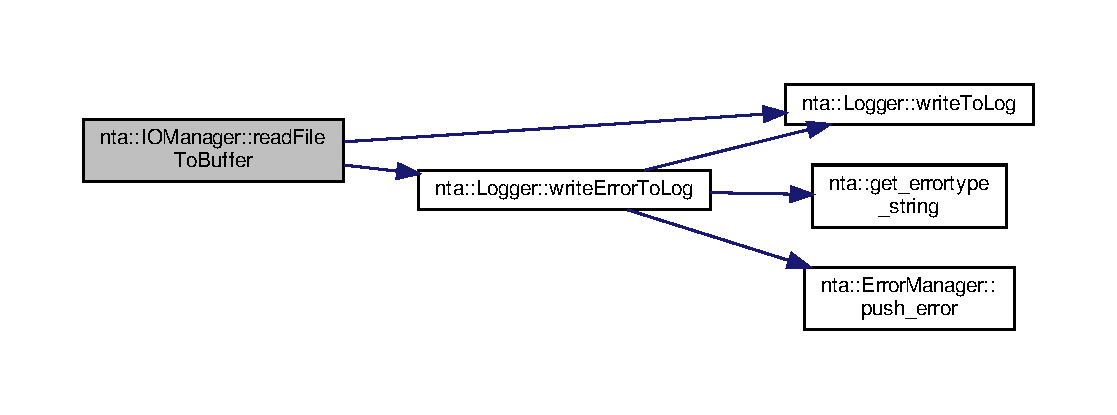
\includegraphics[width=350pt]{d2/d54/classnta_1_1IOManager_abbfd9da05b22aa488043a19344d38e0a_cgraph}
\end{center}
\end{figure}


The documentation for this class was generated from the following files\+:\begin{DoxyCompactItemize}
\item 
include/nta/I\+O\+Manager.\+h\item 
src/I\+O\+Manager.\+cpp\end{DoxyCompactItemize}

\hypertarget{classnta_1_1utils_1_1Json_1_1iterator}{}\section{nta\+:\+:utils\+:\+:Json\+:\+:iterator$<$ c $>$ Class Template Reference}
\label{classnta_1_1utils_1_1Json_1_1iterator}\index{nta\+::utils\+::\+Json\+::iterator$<$ c $>$@{nta\+::utils\+::\+Json\+::iterator$<$ c $>$}}


{\ttfamily \#include $<$json.\+h$>$}

\subsection*{Public Types}
\begin{DoxyCompactItemize}
\item 
\mbox{\Hypertarget{classnta_1_1utils_1_1Json_1_1iterator_a4f7a3947bf631f014b6af1fba6e55650}\label{classnta_1_1utils_1_1Json_1_1iterator_a4f7a3947bf631f014b6af1fba6e55650}} 
using {\bfseries value\+\_\+type} = typename std\+::conditional$<$ c, const \hyperlink{classnta_1_1utils_1_1Json}{Json}, \hyperlink{classnta_1_1utils_1_1Json}{Json} $>$\+::type
\item 
\mbox{\Hypertarget{classnta_1_1utils_1_1Json_1_1iterator_a1de62fed92f8ed1612fa584b191dce13}\label{classnta_1_1utils_1_1Json_1_1iterator_a1de62fed92f8ed1612fa584b191dce13}} 
using {\bfseries difference\+\_\+type} = std\+::ptrdiff\+\_\+t
\item 
\mbox{\Hypertarget{classnta_1_1utils_1_1Json_1_1iterator_a9724b64941d2b7097a56ae3bd26f6d6c}\label{classnta_1_1utils_1_1Json_1_1iterator_a9724b64941d2b7097a56ae3bd26f6d6c}} 
using {\bfseries pointer} = typename std\+::conditional$<$ c, const \hyperlink{classnta_1_1utils_1_1Json}{Json} $\ast$, \hyperlink{classnta_1_1utils_1_1Json}{Json} $\ast$ $>$\+::type
\item 
\mbox{\Hypertarget{classnta_1_1utils_1_1Json_1_1iterator_a0b2b7e34047092ab09ea3e6217cd52a9}\label{classnta_1_1utils_1_1Json_1_1iterator_a0b2b7e34047092ab09ea3e6217cd52a9}} 
using {\bfseries reference} = typename std\+::conditional$<$ c, const \hyperlink{classnta_1_1utils_1_1Json}{Json} \&, \hyperlink{classnta_1_1utils_1_1Json}{Json} \& $>$\+::type
\item 
\mbox{\Hypertarget{classnta_1_1utils_1_1Json_1_1iterator_a09be53898b73b32af274b07393dc9ce8}\label{classnta_1_1utils_1_1Json_1_1iterator_a09be53898b73b32af274b07393dc9ce8}} 
using {\bfseries iterator\+\_\+category} = std\+::bidirectional\+\_\+iterator\+\_\+tag
\end{DoxyCompactItemize}
\subsection*{Public Member Functions}
\begin{DoxyCompactItemize}
\item 
\mbox{\Hypertarget{classnta_1_1utils_1_1Json_1_1iterator_a6feab6e42b8715108b66903f03f6057c}\label{classnta_1_1utils_1_1Json_1_1iterator_a6feab6e42b8715108b66903f03f6057c}} 
{\bfseries iterator} (pointer json)
\item 
\mbox{\Hypertarget{classnta_1_1utils_1_1Json_1_1iterator_ac0600fba7bf18f0a137923480a5c2474}\label{classnta_1_1utils_1_1Json_1_1iterator_ac0600fba7bf18f0a137923480a5c2474}} 
reference {\bfseries operator$\ast$} () const
\item 
\mbox{\Hypertarget{classnta_1_1utils_1_1Json_1_1iterator_aa47fddf615e22f633d2c6e40ca530d25}\label{classnta_1_1utils_1_1Json_1_1iterator_aa47fddf615e22f633d2c6e40ca530d25}} 
pointer {\bfseries operator-\/$>$} () const
\item 
\mbox{\Hypertarget{classnta_1_1utils_1_1Json_1_1iterator_a879a28de0152d11e0ef4b3779906d63d}\label{classnta_1_1utils_1_1Json_1_1iterator_a879a28de0152d11e0ef4b3779906d63d}} 
\hyperlink{classnta_1_1utils_1_1Json_1_1iterator}{iterator} \& {\bfseries operator++} ()
\item 
\mbox{\Hypertarget{classnta_1_1utils_1_1Json_1_1iterator_a7fce204edabbca38ea7617e80e74df12}\label{classnta_1_1utils_1_1Json_1_1iterator_a7fce204edabbca38ea7617e80e74df12}} 
\hyperlink{classnta_1_1utils_1_1Json_1_1iterator}{iterator} {\bfseries operator++} (int)
\item 
\mbox{\Hypertarget{classnta_1_1utils_1_1Json_1_1iterator_a237ca5a76a15dddf6e802aab1cace840}\label{classnta_1_1utils_1_1Json_1_1iterator_a237ca5a76a15dddf6e802aab1cace840}} 
\hyperlink{classnta_1_1utils_1_1Json_1_1iterator}{iterator} \& {\bfseries operator-\/-\/} ()
\item 
\mbox{\Hypertarget{classnta_1_1utils_1_1Json_1_1iterator_aee5842b7d5dcc491b4b11be224ed5377}\label{classnta_1_1utils_1_1Json_1_1iterator_aee5842b7d5dcc491b4b11be224ed5377}} 
\hyperlink{classnta_1_1utils_1_1Json_1_1iterator}{iterator} {\bfseries operator-\/-\/} (int)
\item 
\mbox{\Hypertarget{classnta_1_1utils_1_1Json_1_1iterator_a99e56e5fc1b47c4f94b1fc26e2665b52}\label{classnta_1_1utils_1_1Json_1_1iterator_a99e56e5fc1b47c4f94b1fc26e2665b52}} 
bool {\bfseries operator==} (const \hyperlink{classnta_1_1utils_1_1Json_1_1iterator}{iterator} \&rhs) const
\item 
\mbox{\Hypertarget{classnta_1_1utils_1_1Json_1_1iterator_a19704e34d1c4ce82c453ebcd08937bd9}\label{classnta_1_1utils_1_1Json_1_1iterator_a19704e34d1c4ce82c453ebcd08937bd9}} 
bool {\bfseries operator!=} (const \hyperlink{classnta_1_1utils_1_1Json_1_1iterator}{iterator} \&rhs) const
\item 
\mbox{\Hypertarget{classnta_1_1utils_1_1Json_1_1iterator_a0abc8151c0931f7ff0912de6478d6b63}\label{classnta_1_1utils_1_1Json_1_1iterator_a0abc8151c0931f7ff0912de6478d6b63}} 
std\+::string {\bfseries key} ()
\item 
\mbox{\Hypertarget{classnta_1_1utils_1_1Json_1_1iterator_aa86005b7dab48886c6358633634107ec}\label{classnta_1_1utils_1_1Json_1_1iterator_aa86005b7dab48886c6358633634107ec}} 
reference {\bfseries value} ()
\item 
\mbox{\Hypertarget{classnta_1_1utils_1_1Json_1_1iterator_a28508255d518c92490808787f8484696}\label{classnta_1_1utils_1_1Json_1_1iterator_a28508255d518c92490808787f8484696}} 
void {\bfseries set\+\_\+begin} (\hyperlink{classnta_1_1utils_1_1Json_1_1SetBeginEndKey}{Set\+Begin\+End\+Key} \+\_\+)
\item 
\mbox{\Hypertarget{classnta_1_1utils_1_1Json_1_1iterator_aa4ec95c97de3e953f123e2eeeeb883ef}\label{classnta_1_1utils_1_1Json_1_1iterator_aa4ec95c97de3e953f123e2eeeeb883ef}} 
void {\bfseries set\+\_\+end} (\hyperlink{classnta_1_1utils_1_1Json_1_1SetBeginEndKey}{Set\+Begin\+End\+Key} \+\_\+)
\end{DoxyCompactItemize}
\subsection*{Private Attributes}
\begin{DoxyCompactItemize}
\item 
\mbox{\Hypertarget{classnta_1_1utils_1_1Json_1_1iterator_aac92c76abc16e630ed681ba9ac2f2bce}\label{classnta_1_1utils_1_1Json_1_1iterator_aac92c76abc16e630ed681ba9ac2f2bce}} 
pointer {\bfseries m\+\_\+json}
\item 
\mbox{\Hypertarget{classnta_1_1utils_1_1Json_1_1iterator_a2f232282e680fe262d82b4da48682ff0}\label{classnta_1_1utils_1_1Json_1_1iterator_a2f232282e680fe262d82b4da48682ff0}} 
\begin{tabbing}
xx\=xx\=xx\=xx\=xx\=xx\=xx\=xx\=xx\=\kill
union \{\\
\mbox{\Hypertarget{classnta_1_1utils_1_1Json_1_1iterator_a36a093f85a0d8cc50364669d6954a1d7}\label{classnta_1_1utils_1_1Json_1_1iterator_a36a093f85a0d8cc50364669d6954a1d7}} 
JsonObject::iterator {\bfseries m\_obj\_iter}\\
\mbox{\Hypertarget{classnta_1_1utils_1_1Json_1_1iterator_abde803dad4db632a37d34e56efc60ab0}\label{classnta_1_1utils_1_1Json_1_1iterator_abde803dad4db632a37d34e56efc60ab0}} 
JsonArray::iterator {\bfseries m\_arr\_iter}\\
\}; \\

\end{tabbing}\end{DoxyCompactItemize}


\subsection{Detailed Description}
\subsubsection*{template$<$bool c = 0$>$\newline
class nta\+::utils\+::\+Json\+::iterator$<$ c $>$}

Custom iterator for looping over \hyperlink{classnta_1_1utils_1_1Json}{Json} values For Arrays\+: loops over the elements For Objects\+: loops over the values (keys accessible via Json\+::iterator\+::key()) For anything else (except None)\+: returns the value itself (see tets/json\+\_\+tests.\+cpp) For None\+: empty iterator c=0 gives a regular iterator and c=1 gives a const\+\_\+iterator 

Definition at line 112 of file json.\+h.



Collaboration diagram for nta\+:\+:utils\+:\+:Json\+:\+:iterator$<$ c $>$\+:\nopagebreak
\begin{figure}[H]
\begin{center}
\leavevmode
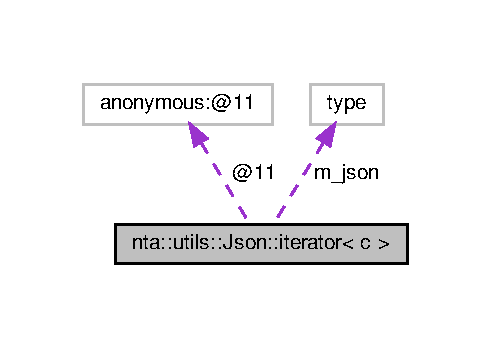
\includegraphics[width=236pt]{da/dc2/classnta_1_1utils_1_1Json_1_1iterator__coll__graph}
\end{center}
\end{figure}


The documentation for this class was generated from the following file\+:\begin{DoxyCompactItemize}
\item 
include/nta/json.\+h\end{DoxyCompactItemize}

\hypertarget{classnta_1_1utils_1_1Json}{}\section{nta\+:\+:utils\+:\+:Json Class Reference}
\label{classnta_1_1utils_1_1Json}\index{nta\+::utils\+::\+Json@{nta\+::utils\+::\+Json}}


{\ttfamily \#include $<$json.\+h$>$}

\subsection*{Classes}
\begin{DoxyCompactItemize}
\item 
class \hyperlink{classnta_1_1utils_1_1Json_1_1iterator}{iterator}
\item 
struct \hyperlink{structnta_1_1utils_1_1Json_1_1JsonToken}{Json\+Token}
\begin{DoxyCompactList}\small\item\em Used for tokenizing strings before parsing them into \hyperlink{classnta_1_1utils_1_1Json}{Json} objects. \end{DoxyCompactList}\item 
union \hyperlink{classnta_1_1utils_1_1Json_d6/d05/unionnta_1_1utils_1_1Json_1_1JsonToken_8____unnamed____}{Json\+Token.\+\_\+\+\_\+unnamed\+\_\+\+\_\+}
\item 
class \hyperlink{classnta_1_1utils_1_1Json_1_1SetBeginEndKey}{Set\+Begin\+End\+Key}
\begin{DoxyCompactList}\small\item\em Key unlocking the set\+\_\+\{begin,end\}() \char`\"{}private\char`\"{} functions of class \hyperlink{classnta_1_1utils_1_1Json_1_1iterator}{Json\+::iterator}. \end{DoxyCompactList}\end{DoxyCompactItemize}
\subsection*{Public Member Functions}
\begin{DoxyCompactItemize}
\item 
\mbox{\Hypertarget{classnta_1_1utils_1_1Json_ac5545c76dd66497cb21edc184f54ffc6}\label{classnta_1_1utils_1_1Json_ac5545c76dd66497cb21edc184f54ffc6}} 
{\bfseries Json} (crstring str)
\item 
\mbox{\Hypertarget{classnta_1_1utils_1_1Json_abf8ba44154d7599b3ca25258c01aa942}\label{classnta_1_1utils_1_1Json_abf8ba44154d7599b3ca25258c01aa942}} 
{\bfseries Json} (const char $\ast$str)
\item 
\mbox{\Hypertarget{classnta_1_1utils_1_1Json_a0460390bd414652905615907ceb3ada7}\label{classnta_1_1utils_1_1Json_a0460390bd414652905615907ceb3ada7}} 
{\bfseries Json} (\hyperlink{classnta_1_1utils_1_1JsonNum}{Json\+Num} num)
\item 
\mbox{\Hypertarget{classnta_1_1utils_1_1Json_acc9de30296d8e0d02b63d57f874ea7bf}\label{classnta_1_1utils_1_1Json_acc9de30296d8e0d02b63d57f874ea7bf}} 
{\bfseries Json} (double num)
\item 
\mbox{\Hypertarget{classnta_1_1utils_1_1Json_aba92a41e2aac44739cf2e77a915c04d6}\label{classnta_1_1utils_1_1Json_aba92a41e2aac44739cf2e77a915c04d6}} 
{\bfseries Json} (int num)
\item 
\mbox{\Hypertarget{classnta_1_1utils_1_1Json_aec39487dbef21bd53b7d4d0bdb2642c2}\label{classnta_1_1utils_1_1Json_aec39487dbef21bd53b7d4d0bdb2642c2}} 
{\bfseries Json} (Json\+Object obj)
\item 
\mbox{\Hypertarget{classnta_1_1utils_1_1Json_aadd85ffafca337080613b36c1e4777f3}\label{classnta_1_1utils_1_1Json_aadd85ffafca337080613b36c1e4777f3}} 
{\bfseries Json} (Json\+Array arr)
\item 
\mbox{\Hypertarget{classnta_1_1utils_1_1Json_a7798a8f8a99468552f505ed3fc2dd86d}\label{classnta_1_1utils_1_1Json_a7798a8f8a99468552f505ed3fc2dd86d}} 
{\bfseries Json} (bool b)
\item 
\mbox{\Hypertarget{classnta_1_1utils_1_1Json_ac2987fdc6d1fc751b9072cc95c09ecd7}\label{classnta_1_1utils_1_1Json_ac2987fdc6d1fc751b9072cc95c09ecd7}} 
{\bfseries Json} (const std\+::initializer\+\_\+list$<$ \hyperlink{classnta_1_1utils_1_1Json}{Json} $>$ \&data)
\item 
\mbox{\Hypertarget{classnta_1_1utils_1_1Json_a77c547bae6a9f97f14e41f235226044c}\label{classnta_1_1utils_1_1Json_a77c547bae6a9f97f14e41f235226044c}} 
{\bfseries Json} (const \hyperlink{classnta_1_1utils_1_1Json}{Json} \&other)
\item 
\mbox{\Hypertarget{classnta_1_1utils_1_1Json_a2c5cf35d9ea355ad8d994857644d215b}\label{classnta_1_1utils_1_1Json_a2c5cf35d9ea355ad8d994857644d215b}} 
{\bfseries Json} (\hyperlink{classnta_1_1utils_1_1Json}{Json} \&\&other)
\item 
\mbox{\Hypertarget{classnta_1_1utils_1_1Json_a2ff34559e1b1189cf528d0f379d2de10}\label{classnta_1_1utils_1_1Json_a2ff34559e1b1189cf528d0f379d2de10}} 
\hyperlink{namespacenta_1_1utils_ac9921c0a3baf86d9facdc4927c66def3}{Json\+Value\+Type} {\bfseries get\+\_\+type} () const
\item 
\mbox{\Hypertarget{classnta_1_1utils_1_1Json_ab6e22f7c4f594c466f1cbc800050a230}\label{classnta_1_1utils_1_1Json_ab6e22f7c4f594c466f1cbc800050a230}} 
bool {\bfseries is\+\_\+string} () const
\item 
\mbox{\Hypertarget{classnta_1_1utils_1_1Json_a1daee4fe2157c815fcc56a709dd696de}\label{classnta_1_1utils_1_1Json_a1daee4fe2157c815fcc56a709dd696de}} 
bool {\bfseries is\+\_\+number} () const
\item 
\mbox{\Hypertarget{classnta_1_1utils_1_1Json_a706bcf555ab4d474ed18871c6d70e2eb}\label{classnta_1_1utils_1_1Json_a706bcf555ab4d474ed18871c6d70e2eb}} 
bool {\bfseries is\+\_\+object} () const
\item 
\mbox{\Hypertarget{classnta_1_1utils_1_1Json_a199bd3270733f1c6d5e69f0bbcad09a5}\label{classnta_1_1utils_1_1Json_a199bd3270733f1c6d5e69f0bbcad09a5}} 
bool {\bfseries is\+\_\+array} () const
\item 
\mbox{\Hypertarget{classnta_1_1utils_1_1Json_a8ad7cc5cd4c4ac8dd18c44792a87794d}\label{classnta_1_1utils_1_1Json_a8ad7cc5cd4c4ac8dd18c44792a87794d}} 
bool {\bfseries is\+\_\+bool} () const
\item 
\mbox{\Hypertarget{classnta_1_1utils_1_1Json_aa065ba60501dde7721468dcfcbd418a5}\label{classnta_1_1utils_1_1Json_aa065ba60501dde7721468dcfcbd418a5}} 
bool {\bfseries is\+\_\+null} () const
\item 
\mbox{\Hypertarget{classnta_1_1utils_1_1Json_a770c5bfc20eab5c6df65e927d526696f}\label{classnta_1_1utils_1_1Json_a770c5bfc20eab5c6df65e927d526696f}} 
std\+::string {\bfseries as\+\_\+string} () const
\item 
\mbox{\Hypertarget{classnta_1_1utils_1_1Json_a500ca051d80c21f9f3339db8c3225ae5}\label{classnta_1_1utils_1_1Json_a500ca051d80c21f9f3339db8c3225ae5}} 
\hyperlink{classnta_1_1utils_1_1JsonNum}{Json\+Num} {\bfseries as\+\_\+number} () const
\item 
\mbox{\Hypertarget{classnta_1_1utils_1_1Json_ae8e43e1645fa2ba2e26c56f3a9f5938d}\label{classnta_1_1utils_1_1Json_ae8e43e1645fa2ba2e26c56f3a9f5938d}} 
uint64\+\_\+t {\bfseries as\+\_\+uint} () const
\item 
\mbox{\Hypertarget{classnta_1_1utils_1_1Json_a81ab98ec58659a3c722c165b2f2cad26}\label{classnta_1_1utils_1_1Json_a81ab98ec58659a3c722c165b2f2cad26}} 
int64\+\_\+t {\bfseries as\+\_\+int} () const
\item 
\mbox{\Hypertarget{classnta_1_1utils_1_1Json_ad0654a2845c1957e9e26e0d349190aae}\label{classnta_1_1utils_1_1Json_ad0654a2845c1957e9e26e0d349190aae}} 
double {\bfseries as\+\_\+float} () const
\item 
\mbox{\Hypertarget{classnta_1_1utils_1_1Json_af99b16247ed73aceacea08b1b5a9c08d}\label{classnta_1_1utils_1_1Json_af99b16247ed73aceacea08b1b5a9c08d}} 
double {\bfseries as\+\_\+double} () const
\item 
\mbox{\Hypertarget{classnta_1_1utils_1_1Json_a9ff2984098105b164e0110684cd6d4f1}\label{classnta_1_1utils_1_1Json_a9ff2984098105b164e0110684cd6d4f1}} 
Json\+Object {\bfseries as\+\_\+object} () const
\item 
\mbox{\Hypertarget{classnta_1_1utils_1_1Json_ab42df34419fb892f2210527f01a82154}\label{classnta_1_1utils_1_1Json_ab42df34419fb892f2210527f01a82154}} 
Json\+Array {\bfseries as\+\_\+array} () const
\item 
\mbox{\Hypertarget{classnta_1_1utils_1_1Json_ad6d8da49cb8355c956ab75faa79cad2c}\label{classnta_1_1utils_1_1Json_ad6d8da49cb8355c956ab75faa79cad2c}} 
bool {\bfseries as\+\_\+bool} () const
\item 
\mbox{\Hypertarget{classnta_1_1utils_1_1Json_a2f3d19984b11f942d0725f76e8e9a165}\label{classnta_1_1utils_1_1Json_a2f3d19984b11f942d0725f76e8e9a165}} 
std\+::size\+\_\+t {\bfseries size} () const
\item 
\mbox{\Hypertarget{classnta_1_1utils_1_1Json_af306c2488e1a4ea456b37dc2dc1205f1}\label{classnta_1_1utils_1_1Json_af306c2488e1a4ea456b37dc2dc1205f1}} 
bool {\bfseries is\+\_\+empty} () const
\item 
bool \hyperlink{classnta_1_1utils_1_1Json_a19f47693bafb5d8e0fe384e0357d0da1}{resize} (std\+::size\+\_\+t size)
\item 
bool \hyperlink{classnta_1_1utils_1_1Json_a2015e471fd47c1a077ca752c9b1fabbd}{push\+\_\+back} (const \hyperlink{classnta_1_1utils_1_1Json}{Json} \&val)
\item 
\mbox{\Hypertarget{classnta_1_1utils_1_1Json_aba3c346a598ddeaec56f016be3da6c50}\label{classnta_1_1utils_1_1Json_aba3c346a598ddeaec56f016be3da6c50}} 
\hyperlink{classnta_1_1utils_1_1Json}{Json} \& \hyperlink{classnta_1_1utils_1_1Json_aba3c346a598ddeaec56f016be3da6c50}{front} ()
\begin{DoxyCompactList}\small\item\em Returns first element if this is an array. \end{DoxyCompactList}\item 
\mbox{\Hypertarget{classnta_1_1utils_1_1Json_a5ac0dc1f03cedaae9944fb7ff71e3893}\label{classnta_1_1utils_1_1Json_a5ac0dc1f03cedaae9944fb7ff71e3893}} 
\hyperlink{classnta_1_1utils_1_1Json}{Json} \& \hyperlink{classnta_1_1utils_1_1Json_a5ac0dc1f03cedaae9944fb7ff71e3893}{back} ()
\begin{DoxyCompactList}\small\item\em Returns last element if this is an array. \end{DoxyCompactList}\item 
\hyperlink{classnta_1_1utils_1_1Json}{Json} \& \hyperlink{classnta_1_1utils_1_1Json_ac33a8a65bdfaff7c365f99c9ca71eeab}{merge} (const \hyperlink{classnta_1_1utils_1_1Json}{Json} \&other)
\item 
std\+::string \hyperlink{classnta_1_1utils_1_1Json_ab0e60f7a55d12aab005d420c8f924035}{dump} (std\+::size\+\_\+t indent=0, std\+::size\+\_\+t offset=0) const
\item 
\mbox{\Hypertarget{classnta_1_1utils_1_1Json_a8b160dd0764464cafc047b185fdbc2f1}\label{classnta_1_1utils_1_1Json_a8b160dd0764464cafc047b185fdbc2f1}} 
{\bfseries operator std\+::string} () const
\item 
\mbox{\Hypertarget{classnta_1_1utils_1_1Json_aa1d29487b097a1485c83c1f153e6b1ef}\label{classnta_1_1utils_1_1Json_aa1d29487b097a1485c83c1f153e6b1ef}} 
{\bfseries operator Json\+Num} () const
\item 
\mbox{\Hypertarget{classnta_1_1utils_1_1Json_a40268cb84b0556e07dd9184a98632f5b}\label{classnta_1_1utils_1_1Json_a40268cb84b0556e07dd9184a98632f5b}} 
{\bfseries operator uint64\+\_\+t} () const
\item 
\mbox{\Hypertarget{classnta_1_1utils_1_1Json_a06d392cd9356cacdfd356fcb16161220}\label{classnta_1_1utils_1_1Json_a06d392cd9356cacdfd356fcb16161220}} 
{\bfseries operator int64\+\_\+t} () const
\item 
\mbox{\Hypertarget{classnta_1_1utils_1_1Json_a68ad0d74dc88bb726bbe4245097ec209}\label{classnta_1_1utils_1_1Json_a68ad0d74dc88bb726bbe4245097ec209}} 
{\bfseries operator int} () const
\item 
\mbox{\Hypertarget{classnta_1_1utils_1_1Json_a7a3b26250aeaa82f9ab0c03a80082a0b}\label{classnta_1_1utils_1_1Json_a7a3b26250aeaa82f9ab0c03a80082a0b}} 
{\bfseries operator float} () const
\item 
\mbox{\Hypertarget{classnta_1_1utils_1_1Json_aa008316811bc941ea29073ae46a358b4}\label{classnta_1_1utils_1_1Json_aa008316811bc941ea29073ae46a358b4}} 
{\bfseries operator double} () const
\item 
\mbox{\Hypertarget{classnta_1_1utils_1_1Json_a5511be349de94fa21d72582d86429d53}\label{classnta_1_1utils_1_1Json_a5511be349de94fa21d72582d86429d53}} 
{\bfseries operator Json\+Object} () const
\item 
\mbox{\Hypertarget{classnta_1_1utils_1_1Json_aed69f0d4f5090100d9e1e8d5df0f01ac}\label{classnta_1_1utils_1_1Json_aed69f0d4f5090100d9e1e8d5df0f01ac}} 
{\bfseries operator Json\+Array} () const
\item 
\mbox{\Hypertarget{classnta_1_1utils_1_1Json_ab1284552f59903991ed0ad31fc2ad91f}\label{classnta_1_1utils_1_1Json_ab1284552f59903991ed0ad31fc2ad91f}} 
{\bfseries operator bool} () const
\item 
\mbox{\Hypertarget{classnta_1_1utils_1_1Json_a3f673cffc8988a0d3d68e081dd3360ed}\label{classnta_1_1utils_1_1Json_a3f673cffc8988a0d3d68e081dd3360ed}} 
\hyperlink{classnta_1_1utils_1_1Json}{Json} \& {\bfseries operator=} (const \hyperlink{classnta_1_1utils_1_1Json}{Json} \&other)
\item 
\mbox{\Hypertarget{classnta_1_1utils_1_1Json_a52fbe1664fe12b582c5e2b18cc2cfdc8}\label{classnta_1_1utils_1_1Json_a52fbe1664fe12b582c5e2b18cc2cfdc8}} 
\hyperlink{classnta_1_1utils_1_1Json}{Json} \& {\bfseries operator=} (\hyperlink{classnta_1_1utils_1_1Json}{Json} \&\&other)
\item 
\mbox{\Hypertarget{classnta_1_1utils_1_1Json_a5ef5f3aea0472da1682d1a6757073491}\label{classnta_1_1utils_1_1Json_a5ef5f3aea0472da1682d1a6757073491}} 
bool {\bfseries operator==} (const \hyperlink{classnta_1_1utils_1_1Json}{Json} \&other) const
\item 
\mbox{\Hypertarget{classnta_1_1utils_1_1Json_a97b88c3b36c4ea7640074b676abe7a89}\label{classnta_1_1utils_1_1Json_a97b88c3b36c4ea7640074b676abe7a89}} 
bool {\bfseries operator!=} (const \hyperlink{classnta_1_1utils_1_1Json}{Json} \&other) const
\item 
\mbox{\Hypertarget{classnta_1_1utils_1_1Json_a70675599c2188f99903ac40f30a10615}\label{classnta_1_1utils_1_1Json_a70675599c2188f99903ac40f30a10615}} 
bool {\bfseries operator==} (const std\+::string \&other) const
\item 
\mbox{\Hypertarget{classnta_1_1utils_1_1Json_a8f4bfd013e4e02783f2283506590b5f6}\label{classnta_1_1utils_1_1Json_a8f4bfd013e4e02783f2283506590b5f6}} 
bool {\bfseries operator!=} (const std\+::string \&other) const
\item 
\mbox{\Hypertarget{classnta_1_1utils_1_1Json_a5ed2511971393973e89721cdebefd839}\label{classnta_1_1utils_1_1Json_a5ed2511971393973e89721cdebefd839}} 
bool {\bfseries operator==} (const char $\ast$other) const
\item 
\mbox{\Hypertarget{classnta_1_1utils_1_1Json_a8ff4372a5deec91c76406aa9db38fb29}\label{classnta_1_1utils_1_1Json_a8ff4372a5deec91c76406aa9db38fb29}} 
bool {\bfseries operator!=} (const char $\ast$other) const
\item 
\mbox{\Hypertarget{classnta_1_1utils_1_1Json_afd19449d8c0ef71a4a5e3544841f9e9b}\label{classnta_1_1utils_1_1Json_afd19449d8c0ef71a4a5e3544841f9e9b}} 
bool {\bfseries operator==} (const \hyperlink{classnta_1_1utils_1_1JsonNum}{Json\+Num} \&other) const
\item 
\mbox{\Hypertarget{classnta_1_1utils_1_1Json_a0fe90155a63c4de53af0d2568e526701}\label{classnta_1_1utils_1_1Json_a0fe90155a63c4de53af0d2568e526701}} 
bool {\bfseries operator!=} (const \hyperlink{classnta_1_1utils_1_1JsonNum}{Json\+Num} \&other) const
\item 
\mbox{\Hypertarget{classnta_1_1utils_1_1Json_a7508ebbd9d94e223b75d942056b6f1d3}\label{classnta_1_1utils_1_1Json_a7508ebbd9d94e223b75d942056b6f1d3}} 
bool {\bfseries operator==} (const int \&other) const
\item 
\mbox{\Hypertarget{classnta_1_1utils_1_1Json_abd71013faafbf7ed1d0c2eb13ef22102}\label{classnta_1_1utils_1_1Json_abd71013faafbf7ed1d0c2eb13ef22102}} 
bool {\bfseries operator!=} (const int \&other) const
\item 
\mbox{\Hypertarget{classnta_1_1utils_1_1Json_a07c84e02229b829d3ce687a47251c28e}\label{classnta_1_1utils_1_1Json_a07c84e02229b829d3ce687a47251c28e}} 
bool {\bfseries operator==} (const Json\+Object \&other) const
\item 
\mbox{\Hypertarget{classnta_1_1utils_1_1Json_a2c47bda59351fc39af7d01af617c8e51}\label{classnta_1_1utils_1_1Json_a2c47bda59351fc39af7d01af617c8e51}} 
bool {\bfseries operator!=} (const Json\+Object \&other) const
\item 
\mbox{\Hypertarget{classnta_1_1utils_1_1Json_a4f8c29566c86919ab1693e4ab709a1b5}\label{classnta_1_1utils_1_1Json_a4f8c29566c86919ab1693e4ab709a1b5}} 
bool {\bfseries operator==} (const Json\+Array \&other) const
\item 
\mbox{\Hypertarget{classnta_1_1utils_1_1Json_a45778e95342f5b95a9f69273eb481f48}\label{classnta_1_1utils_1_1Json_a45778e95342f5b95a9f69273eb481f48}} 
bool {\bfseries operator!=} (const Json\+Array \&other) const
\item 
\mbox{\Hypertarget{classnta_1_1utils_1_1Json_a5a66e88580ae3c456d16d8ec4d2d4556}\label{classnta_1_1utils_1_1Json_a5a66e88580ae3c456d16d8ec4d2d4556}} 
bool {\bfseries operator==} (const bool \&other) const
\item 
\mbox{\Hypertarget{classnta_1_1utils_1_1Json_a05bb2f19f7b4239c1bbe718e8350c8d0}\label{classnta_1_1utils_1_1Json_a05bb2f19f7b4239c1bbe718e8350c8d0}} 
bool {\bfseries operator!=} (const bool \&other) const
\item 
\hyperlink{classnta_1_1utils_1_1Json}{Json} \& \hyperlink{classnta_1_1utils_1_1Json_adf2d340a2bf7d59c537e398a1be66cf7}{operator\mbox{[}$\,$\mbox{]}} (crstring key)
\begin{DoxyCompactList}\small\item\em When m\+\_\+type == N\+O\+NE, first converts this into an Object. \end{DoxyCompactList}\item 
\hyperlink{classnta_1_1utils_1_1Json}{Json} \& \hyperlink{classnta_1_1utils_1_1Json_ab3b51a07ebed90330c98fd8e20785781}{operator\mbox{[}$\,$\mbox{]}} (crstring key) const
\item 
\mbox{\Hypertarget{classnta_1_1utils_1_1Json_a4dcba3e4e113c3204212fea031725c9c}\label{classnta_1_1utils_1_1Json_a4dcba3e4e113c3204212fea031725c9c}} 
\hyperlink{classnta_1_1utils_1_1Json}{Json} \& {\bfseries operator\mbox{[}$\,$\mbox{]}} (const char $\ast$key)
\item 
\mbox{\Hypertarget{classnta_1_1utils_1_1Json_adf46f886ad73e0cacb7d0e5cc40841b3}\label{classnta_1_1utils_1_1Json_adf46f886ad73e0cacb7d0e5cc40841b3}} 
\hyperlink{classnta_1_1utils_1_1Json}{Json} \& {\bfseries operator\mbox{[}$\,$\mbox{]}} (const char $\ast$key) const
\item 
\hyperlink{classnta_1_1utils_1_1Json}{Json} \& \hyperlink{classnta_1_1utils_1_1Json_a236b5885612b74c21fbad169b21eaf55}{operator\mbox{[}$\,$\mbox{]}} (std\+::size\+\_\+t idx)
\item 
\hyperlink{classnta_1_1utils_1_1Json}{Json} \& \hyperlink{classnta_1_1utils_1_1Json_a893f191111e604995488d147aaa711f8}{operator\mbox{[}$\,$\mbox{]}} (std\+::size\+\_\+t idx) const
\item 
\mbox{\Hypertarget{classnta_1_1utils_1_1Json_a7d094a2061036a579a63923ae30171a4}\label{classnta_1_1utils_1_1Json_a7d094a2061036a579a63923ae30171a4}} 
\hyperlink{classnta_1_1utils_1_1Json}{Json} \& {\bfseries operator\mbox{[}$\,$\mbox{]}} (int idx)
\item 
\mbox{\Hypertarget{classnta_1_1utils_1_1Json_aba70b2f342f889783480ef72c606b240}\label{classnta_1_1utils_1_1Json_aba70b2f342f889783480ef72c606b240}} 
\hyperlink{classnta_1_1utils_1_1Json}{Json} \& {\bfseries operator\mbox{[}$\,$\mbox{]}} (int idx) const
\item 
\mbox{\Hypertarget{classnta_1_1utils_1_1Json_a9f001e2bb1883915bee5fa9a0df8258b}\label{classnta_1_1utils_1_1Json_a9f001e2bb1883915bee5fa9a0df8258b}} 
\hyperlink{classnta_1_1utils_1_1Json_1_1iterator}{iterator}$<$ 0 $>$ {\bfseries begin} ()
\item 
\mbox{\Hypertarget{classnta_1_1utils_1_1Json_a712d6d5350c2390677e3aab6b9ce2b80}\label{classnta_1_1utils_1_1Json_a712d6d5350c2390677e3aab6b9ce2b80}} 
\hyperlink{classnta_1_1utils_1_1Json_1_1iterator}{iterator}$<$ 1 $>$ {\bfseries cbegin} () const
\item 
\mbox{\Hypertarget{classnta_1_1utils_1_1Json_a37ac10b5f6baad85be2625c1efbccf74}\label{classnta_1_1utils_1_1Json_a37ac10b5f6baad85be2625c1efbccf74}} 
\hyperlink{classnta_1_1utils_1_1Json_1_1iterator}{iterator}$<$ 0 $>$ {\bfseries end} ()
\item 
\mbox{\Hypertarget{classnta_1_1utils_1_1Json_a58fc30fc1f2e1498093070c848f63847}\label{classnta_1_1utils_1_1Json_a58fc30fc1f2e1498093070c848f63847}} 
\hyperlink{classnta_1_1utils_1_1Json_1_1iterator}{iterator}$<$ 1 $>$ {\bfseries cend} () const
\end{DoxyCompactItemize}
\subsection*{Static Public Member Functions}
\begin{DoxyCompactItemize}
\item 
\mbox{\Hypertarget{classnta_1_1utils_1_1Json_add20ea70d84582b2446dc53be92ac50c}\label{classnta_1_1utils_1_1Json_add20ea70d84582b2446dc53be92ac50c}} 
static \hyperlink{classnta_1_1utils_1_1Json}{Json} {\bfseries string} (crstring str)
\item 
\mbox{\Hypertarget{classnta_1_1utils_1_1Json_a84415d3c83a91fed0689276c538e886e}\label{classnta_1_1utils_1_1Json_a84415d3c83a91fed0689276c538e886e}} 
static \hyperlink{classnta_1_1utils_1_1Json}{Json} {\bfseries string} (const char $\ast$str)
\item 
\mbox{\Hypertarget{classnta_1_1utils_1_1Json_a5e985dfb6c9148df9401b89265a0852c}\label{classnta_1_1utils_1_1Json_a5e985dfb6c9148df9401b89265a0852c}} 
static \hyperlink{classnta_1_1utils_1_1Json}{Json} {\bfseries number} (\hyperlink{classnta_1_1utils_1_1JsonNum}{Json\+Num} num)
\item 
\mbox{\Hypertarget{classnta_1_1utils_1_1Json_ac5e29dac15a59829e1f6e927fe8cde5d}\label{classnta_1_1utils_1_1Json_ac5e29dac15a59829e1f6e927fe8cde5d}} 
static \hyperlink{classnta_1_1utils_1_1Json}{Json} {\bfseries object} (Json\+Object obj)
\item 
\mbox{\Hypertarget{classnta_1_1utils_1_1Json_a2a99930e97628a41cf647cbdb52d8a76}\label{classnta_1_1utils_1_1Json_a2a99930e97628a41cf647cbdb52d8a76}} 
static \hyperlink{classnta_1_1utils_1_1Json}{Json} {\bfseries array} (Json\+Array arr)
\item 
\mbox{\Hypertarget{classnta_1_1utils_1_1Json_a023ca360caf8dbb385a805b0c21c98c3}\label{classnta_1_1utils_1_1Json_a023ca360caf8dbb385a805b0c21c98c3}} 
static \hyperlink{classnta_1_1utils_1_1Json}{Json} {\bfseries boolean} (bool boolean)
\item 
\mbox{\Hypertarget{classnta_1_1utils_1_1Json_a89aa8497a420120774eec8335a6bf42e}\label{classnta_1_1utils_1_1Json_a89aa8497a420120774eec8335a6bf42e}} 
static \hyperlink{classnta_1_1utils_1_1Json}{Json} {\bfseries null} ()
\item 
\mbox{\Hypertarget{classnta_1_1utils_1_1Json_ac4e9f86cd5c15c077f993d86a68eb044}\label{classnta_1_1utils_1_1Json_ac4e9f86cd5c15c077f993d86a68eb044}} 
static \hyperlink{classnta_1_1utils_1_1Json}{Json} \hyperlink{classnta_1_1utils_1_1Json_ac4e9f86cd5c15c077f993d86a68eb044}{parse} (crstring json)
\begin{DoxyCompactList}\small\item\em Parses \hyperlink{classnta_1_1utils_1_1Json}{Json} value from a string. \end{DoxyCompactList}\item 
\mbox{\Hypertarget{classnta_1_1utils_1_1Json_a1f9c21e0ba80e348e2c6c19070cbc45e}\label{classnta_1_1utils_1_1Json_a1f9c21e0ba80e348e2c6c19070cbc45e}} 
static \hyperlink{classnta_1_1utils_1_1Json}{Json} {\bfseries from\+\_\+file} (crstring path)
\end{DoxyCompactItemize}
\subsection*{Private Types}
\begin{DoxyCompactItemize}
\item 
\mbox{\Hypertarget{classnta_1_1utils_1_1Json_aa2dc580b7a31ea9cef4226527b4599f3}\label{classnta_1_1utils_1_1Json_aa2dc580b7a31ea9cef4226527b4599f3}} 
enum {\bfseries Json\+Token\+Type} \{ {\bfseries S\+Y\+M\+B\+OL}, 
{\bfseries N\+U\+M\+T\+KN}
 \}
\end{DoxyCompactItemize}
\subsection*{Private Member Functions}
\begin{DoxyCompactItemize}
\item 
\mbox{\Hypertarget{classnta_1_1utils_1_1Json_ac86f6995528403eb265d2cd8a46ed4eb}\label{classnta_1_1utils_1_1Json_ac86f6995528403eb265d2cd8a46ed4eb}} 
{\bfseries Json} (\hyperlink{namespacenta_1_1utils_ac9921c0a3baf86d9facdc4927c66def3}{Json\+Value\+Type} type)
\end{DoxyCompactItemize}
\subsection*{Static Private Member Functions}
\begin{DoxyCompactItemize}
\item 
\mbox{\Hypertarget{classnta_1_1utils_1_1Json_a085ef4e12b6ac83ef239425037b5bf73}\label{classnta_1_1utils_1_1Json_a085ef4e12b6ac83ef239425037b5bf73}} 
static bool \hyperlink{classnta_1_1utils_1_1Json_a085ef4e12b6ac83ef239425037b5bf73}{lex\+\_\+string} (std\+::string \&str, \hyperlink{structnta_1_1utils_1_1Json_1_1JsonToken}{Json\+Token} \&ret)
\begin{DoxyCompactList}\small\item\em Attempts to retreive a string token from the beginning of str. \end{DoxyCompactList}\item 
\mbox{\Hypertarget{classnta_1_1utils_1_1Json_a85d932ecf9fc69f93af5da7349a8e265}\label{classnta_1_1utils_1_1Json_a85d932ecf9fc69f93af5da7349a8e265}} 
static bool \hyperlink{classnta_1_1utils_1_1Json_a85d932ecf9fc69f93af5da7349a8e265}{lex\+\_\+number} (std\+::string \&str, \hyperlink{structnta_1_1utils_1_1Json_1_1JsonToken}{Json\+Token} \&ret)
\begin{DoxyCompactList}\small\item\em Attempts to retreive a number token from the beginning of str. \end{DoxyCompactList}\item 
\mbox{\Hypertarget{classnta_1_1utils_1_1Json_af563232c6a9334fe69f05ae33ee76573}\label{classnta_1_1utils_1_1Json_af563232c6a9334fe69f05ae33ee76573}} 
static bool \hyperlink{classnta_1_1utils_1_1Json_af563232c6a9334fe69f05ae33ee76573}{lex\+\_\+bool} (std\+::string \&str, \hyperlink{structnta_1_1utils_1_1Json_1_1JsonToken}{Json\+Token} \&ret)
\begin{DoxyCompactList}\small\item\em Attempts to retreive a boolean token from the beginning of str. \end{DoxyCompactList}\item 
\mbox{\Hypertarget{classnta_1_1utils_1_1Json_aea0272293c585f0d30811afe6a43917b}\label{classnta_1_1utils_1_1Json_aea0272293c585f0d30811afe6a43917b}} 
static bool \hyperlink{classnta_1_1utils_1_1Json_aea0272293c585f0d30811afe6a43917b}{lex\+\_\+null} (std\+::string \&str, \hyperlink{structnta_1_1utils_1_1Json_1_1JsonToken}{Json\+Token} \&ret)
\begin{DoxyCompactList}\small\item\em Attempts to retreive a null token from the beginning of str. \end{DoxyCompactList}\item 
static std\+::queue$<$ \hyperlink{structnta_1_1utils_1_1Json_1_1JsonToken}{Json\+Token} $>$ \hyperlink{classnta_1_1utils_1_1Json_a905d67b125a7aadd771bb74a1bb63f34}{tokenize} (std\+::string curr)
\begin{DoxyCompactList}\small\item\em Converts curr into a stream of tokens. \end{DoxyCompactList}\item 
\mbox{\Hypertarget{classnta_1_1utils_1_1Json_a6952edc41983e76a7e548d9c426bc680}\label{classnta_1_1utils_1_1Json_a6952edc41983e76a7e548d9c426bc680}} 
static \hyperlink{classnta_1_1utils_1_1Json}{Json} \hyperlink{classnta_1_1utils_1_1Json_a6952edc41983e76a7e548d9c426bc680}{parse\+\_\+tokens} (std\+::queue$<$ \hyperlink{structnta_1_1utils_1_1Json_1_1JsonToken}{Json\+Token} $>$ \&tokens)
\begin{DoxyCompactList}\small\item\em Converts stream of tokens into a \hyperlink{classnta_1_1utils_1_1Json}{Json} value. \end{DoxyCompactList}\end{DoxyCompactItemize}
\subsection*{Private Attributes}
\begin{DoxyCompactItemize}
\item 
\mbox{\Hypertarget{classnta_1_1utils_1_1Json_ab4a7cc232d1c4ba37f9dcb35f0ac5417}\label{classnta_1_1utils_1_1Json_ab4a7cc232d1c4ba37f9dcb35f0ac5417}} 
\hyperlink{namespacenta_1_1utils_ac9921c0a3baf86d9facdc4927c66def3}{Json\+Value\+Type} {\bfseries m\+\_\+type}
\item 
\mbox{\Hypertarget{classnta_1_1utils_1_1Json_a6a4d3082c4d8f9987cb8ce281b87744d}\label{classnta_1_1utils_1_1Json_a6a4d3082c4d8f9987cb8ce281b87744d}} 
\begin{tabbing}
xx\=xx\=xx\=xx\=xx\=xx\=xx\=xx\=xx\=\kill
union \{\\
\mbox{\Hypertarget{classnta_1_1utils_1_1Json_ad70123a682fef22afdcf75d20d028e3e}\label{classnta_1_1utils_1_1Json_ad70123a682fef22afdcf75d20d028e3e}} 
char $\ast$ {\bfseries m\_str}\\
\mbox{\Hypertarget{classnta_1_1utils_1_1Json_aad4acf20f0eef3112e633df34b799b5a}\label{classnta_1_1utils_1_1Json_aad4acf20f0eef3112e633df34b799b5a}} 
\hyperlink{classnta_1_1utils_1_1JsonNum}{JsonNum} {\bfseries m\_num}\\
\mbox{\Hypertarget{classnta_1_1utils_1_1Json_a15a631f10ecc26ba5fba053140bc7500}\label{classnta_1_1utils_1_1Json_a15a631f10ecc26ba5fba053140bc7500}} 
JsonObject $\ast$ {\bfseries m\_obj}\\
\mbox{\Hypertarget{classnta_1_1utils_1_1Json_a1ddb791c97e2d345cad4ad63bcb38b6b}\label{classnta_1_1utils_1_1Json_a1ddb791c97e2d345cad4ad63bcb38b6b}} 
JsonArray $\ast$ {\bfseries m\_arr}\\
\mbox{\Hypertarget{classnta_1_1utils_1_1Json_a4ca79ced26d31b35a7d2f9e0fc8ec347}\label{classnta_1_1utils_1_1Json_a4ca79ced26d31b35a7d2f9e0fc8ec347}} 
bool {\bfseries m\_bool}\\
\}; \\

\end{tabbing}\end{DoxyCompactItemize}


\subsection{Detailed Description}
\begin{DoxyRefDesc}{Todo}
\item[\hyperlink{todo__todo000006}{Todo}]Make as\+\_\+$\ast$ functions safer and more versatile An arbitrary \hyperlink{classnta_1_1utils_1_1Json}{Json} value \end{DoxyRefDesc}


Definition at line 95 of file json.\+h.



Collaboration diagram for nta\+:\+:utils\+:\+:Json\+:\nopagebreak
\begin{figure}[H]
\begin{center}
\leavevmode
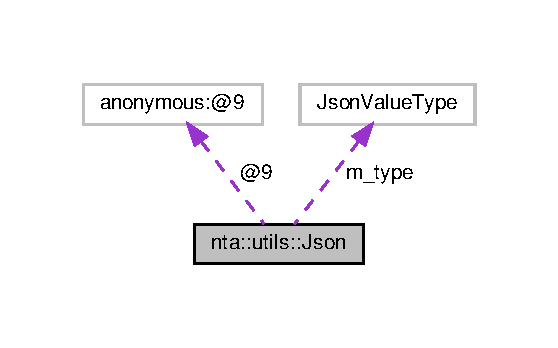
\includegraphics[width=268pt]{d2/de6/classnta_1_1utils_1_1Json__coll__graph}
\end{center}
\end{figure}


\subsection{Class Documentation}
\index{nta\+::utils\+::\+Json\+::\+Json\+Token.\+\_\+\+\_\+unnamed\+\_\+\+\_\+@{nta\+::utils\+::\+Json\+::\+Json\+Token.\+\_\+\+\_\+unnamed\+\_\+\+\_\+}}\label{unionnta_1_1utils_1_1Json_1_1JsonToken_8____unnamed____}
\Hypertarget{classnta_1_1utils_1_1Json_unionnta_1_1utils_1_1Json_1_1JsonToken_8____unnamed____}
\subsubsection{union nta\+:\+:utils\+:\+:Json\+:\+:Json\+Token.\+\_\+\+\_\+unnamed\+\_\+\+\_\+}


Definition at line 254 of file json.\+h.

\begin{DoxyFields}{Class Members}
\mbox{\Hypertarget{classnta_1_1utils_1_1Json_a0fc3cfbc27e91ea60a787de13dae3e3c}\label{classnta_1_1utils_1_1Json_a0fc3cfbc27e91ea60a787de13dae3e3c}} 
\hyperlink{classnta_1_1utils_1_1JsonNum}{JsonNum}&
num&
\\
\hline

\mbox{\Hypertarget{classnta_1_1utils_1_1Json_a341be97d9aff90c9978347f66f945b77}\label{classnta_1_1utils_1_1Json_a341be97d9aff90c9978347f66f945b77}} 
char $\ast$&
str&
\\
\hline

\end{DoxyFields}


\subsection{Member Function Documentation}
\mbox{\Hypertarget{classnta_1_1utils_1_1Json_ab0e60f7a55d12aab005d420c8f924035}\label{classnta_1_1utils_1_1Json_ab0e60f7a55d12aab005d420c8f924035}} 
\index{nta\+::utils\+::\+Json@{nta\+::utils\+::\+Json}!dump@{dump}}
\index{dump@{dump}!nta\+::utils\+::\+Json@{nta\+::utils\+::\+Json}}
\subsubsection{\texorpdfstring{dump()}{dump()}}
{\footnotesize\ttfamily std\+::string nta\+::utils\+::\+Json\+::dump (\begin{DoxyParamCaption}\item[{std\+::size\+\_\+t}]{indent = {\ttfamily 0},  }\item[{std\+::size\+\_\+t}]{offset = {\ttfamily 0} }\end{DoxyParamCaption}) const}

Returns a string representation of the value Note\+: never set second parameter

\begin{DoxyRefDesc}{Todo}
\item[\hyperlink{todo__todo000024}{Todo}]Clean up code \end{DoxyRefDesc}


Definition at line 185 of file json.\+cpp.

\mbox{\Hypertarget{classnta_1_1utils_1_1Json_ac33a8a65bdfaff7c365f99c9ca71eeab}\label{classnta_1_1utils_1_1Json_ac33a8a65bdfaff7c365f99c9ca71eeab}} 
\index{nta\+::utils\+::\+Json@{nta\+::utils\+::\+Json}!merge@{merge}}
\index{merge@{merge}!nta\+::utils\+::\+Json@{nta\+::utils\+::\+Json}}
\subsubsection{\texorpdfstring{merge()}{merge()}}
{\footnotesize\ttfamily \hyperlink{classnta_1_1utils_1_1Json}{Json} \& nta\+::utils\+::\+Json\+::merge (\begin{DoxyParamCaption}\item[{const \hyperlink{classnta_1_1utils_1_1Json}{Json} \&}]{other }\end{DoxyParamCaption})}

Adds everything stored in other into this Returns this 

Definition at line 149 of file json.\+cpp.

\mbox{\Hypertarget{classnta_1_1utils_1_1Json_adf2d340a2bf7d59c537e398a1be66cf7}\label{classnta_1_1utils_1_1Json_adf2d340a2bf7d59c537e398a1be66cf7}} 
\index{nta\+::utils\+::\+Json@{nta\+::utils\+::\+Json}!operator\mbox{[}\mbox{]}@{operator[]}}
\index{operator\mbox{[}\mbox{]}@{operator[]}!nta\+::utils\+::\+Json@{nta\+::utils\+::\+Json}}
\subsubsection{\texorpdfstring{operator[]()}{operator[]()}\hspace{0.1cm}{\footnotesize\ttfamily [1/4]}}
{\footnotesize\ttfamily \hyperlink{classnta_1_1utils_1_1Json}{Json} \& nta\+::utils\+::\+Json\+::operator\mbox{[}$\,$\mbox{]} (\begin{DoxyParamCaption}\item[{crstring}]{key }\end{DoxyParamCaption})}



When m\+\_\+type == N\+O\+NE, first converts this into an Object. 

\begin{DoxyRefDesc}{Todo}
\item[\hyperlink{todo__todo000018}{Todo}]Signal error if m\+\_\+type != O\+B\+J\+E\+CT \end{DoxyRefDesc}


Definition at line 84 of file json.\+cpp.

\mbox{\Hypertarget{classnta_1_1utils_1_1Json_ab3b51a07ebed90330c98fd8e20785781}\label{classnta_1_1utils_1_1Json_ab3b51a07ebed90330c98fd8e20785781}} 
\index{nta\+::utils\+::\+Json@{nta\+::utils\+::\+Json}!operator\mbox{[}\mbox{]}@{operator[]}}
\index{operator\mbox{[}\mbox{]}@{operator[]}!nta\+::utils\+::\+Json@{nta\+::utils\+::\+Json}}
\subsubsection{\texorpdfstring{operator[]()}{operator[]()}\hspace{0.1cm}{\footnotesize\ttfamily [2/4]}}
{\footnotesize\ttfamily \hyperlink{classnta_1_1utils_1_1Json}{Json} \& nta\+::utils\+::\+Json\+::operator\mbox{[}$\,$\mbox{]} (\begin{DoxyParamCaption}\item[{crstring}]{key }\end{DoxyParamCaption}) const}

\begin{DoxyRefDesc}{Todo}
\item[\hyperlink{todo__todo000019}{Todo}]Signal error if m\+\_\+type != O\+B\+J\+E\+CT \end{DoxyRefDesc}


Definition at line 92 of file json.\+cpp.

\mbox{\Hypertarget{classnta_1_1utils_1_1Json_a236b5885612b74c21fbad169b21eaf55}\label{classnta_1_1utils_1_1Json_a236b5885612b74c21fbad169b21eaf55}} 
\index{nta\+::utils\+::\+Json@{nta\+::utils\+::\+Json}!operator\mbox{[}\mbox{]}@{operator[]}}
\index{operator\mbox{[}\mbox{]}@{operator[]}!nta\+::utils\+::\+Json@{nta\+::utils\+::\+Json}}
\subsubsection{\texorpdfstring{operator[]()}{operator[]()}\hspace{0.1cm}{\footnotesize\ttfamily [3/4]}}
{\footnotesize\ttfamily \hyperlink{classnta_1_1utils_1_1Json}{Json} \& nta\+::utils\+::\+Json\+::operator\mbox{[}$\,$\mbox{]} (\begin{DoxyParamCaption}\item[{std\+::size\+\_\+t}]{idx }\end{DoxyParamCaption})}

\begin{DoxyRefDesc}{Todo}
\item[\hyperlink{todo__todo000020}{Todo}]Signal error if m\+\_\+type != A\+R\+R\+AY \end{DoxyRefDesc}
\begin{DoxyRefDesc}{Todo}
\item[\hyperlink{todo__todo000021}{Todo}]Signal error if idx is out of bounds \end{DoxyRefDesc}


Definition at line 96 of file json.\+cpp.

\mbox{\Hypertarget{classnta_1_1utils_1_1Json_a893f191111e604995488d147aaa711f8}\label{classnta_1_1utils_1_1Json_a893f191111e604995488d147aaa711f8}} 
\index{nta\+::utils\+::\+Json@{nta\+::utils\+::\+Json}!operator\mbox{[}\mbox{]}@{operator[]}}
\index{operator\mbox{[}\mbox{]}@{operator[]}!nta\+::utils\+::\+Json@{nta\+::utils\+::\+Json}}
\subsubsection{\texorpdfstring{operator[]()}{operator[]()}\hspace{0.1cm}{\footnotesize\ttfamily [4/4]}}
{\footnotesize\ttfamily \hyperlink{classnta_1_1utils_1_1Json}{Json} \& nta\+::utils\+::\+Json\+::operator\mbox{[}$\,$\mbox{]} (\begin{DoxyParamCaption}\item[{std\+::size\+\_\+t}]{idx }\end{DoxyParamCaption}) const}

\begin{DoxyRefDesc}{Todo}
\item[\hyperlink{todo__todo000022}{Todo}]Signal error if m\+\_\+type != A\+R\+R\+AY \end{DoxyRefDesc}
\begin{DoxyRefDesc}{Todo}
\item[\hyperlink{todo__todo000023}{Todo}]Signal error if idx is out of bounds \end{DoxyRefDesc}


Definition at line 105 of file json.\+cpp.

\mbox{\Hypertarget{classnta_1_1utils_1_1Json_a2015e471fd47c1a077ca752c9b1fabbd}\label{classnta_1_1utils_1_1Json_a2015e471fd47c1a077ca752c9b1fabbd}} 
\index{nta\+::utils\+::\+Json@{nta\+::utils\+::\+Json}!push\+\_\+back@{push\+\_\+back}}
\index{push\+\_\+back@{push\+\_\+back}!nta\+::utils\+::\+Json@{nta\+::utils\+::\+Json}}
\subsubsection{\texorpdfstring{push\+\_\+back()}{push\_back()}}
{\footnotesize\ttfamily bool nta\+::utils\+::\+Json\+::push\+\_\+back (\begin{DoxyParamCaption}\item[{const \hyperlink{classnta_1_1utils_1_1Json}{Json} \&}]{val }\end{DoxyParamCaption})}

Returns false if m\+\_\+type != A\+R\+R\+AY (or N\+O\+NE) If m\+\_\+type == N\+O\+NE, converts this into an A\+R\+R\+AY 

Definition at line 127 of file json.\+cpp.



Referenced by parse\+\_\+tokens().

Here is the caller graph for this function\+:\nopagebreak
\begin{figure}[H]
\begin{center}
\leavevmode
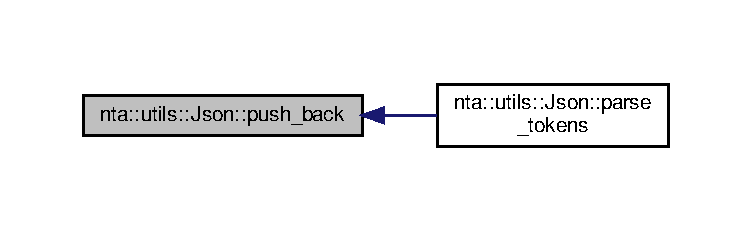
\includegraphics[width=350pt]{d1/d3d/classnta_1_1utils_1_1Json_a2015e471fd47c1a077ca752c9b1fabbd_icgraph}
\end{center}
\end{figure}
\mbox{\Hypertarget{classnta_1_1utils_1_1Json_a19f47693bafb5d8e0fe384e0357d0da1}\label{classnta_1_1utils_1_1Json_a19f47693bafb5d8e0fe384e0357d0da1}} 
\index{nta\+::utils\+::\+Json@{nta\+::utils\+::\+Json}!resize@{resize}}
\index{resize@{resize}!nta\+::utils\+::\+Json@{nta\+::utils\+::\+Json}}
\subsubsection{\texorpdfstring{resize()}{resize()}}
{\footnotesize\ttfamily bool nta\+::utils\+::\+Json\+::resize (\begin{DoxyParamCaption}\item[{std\+::size\+\_\+t}]{size }\end{DoxyParamCaption})}

Returns false if m\+\_\+type is not N\+O\+NE or A\+R\+R\+AY If m\+\_\+type == N\+O\+NE, converts this into an A\+R\+R\+AY 

Definition at line 117 of file json.\+cpp.

\mbox{\Hypertarget{classnta_1_1utils_1_1Json_a905d67b125a7aadd771bb74a1bb63f34}\label{classnta_1_1utils_1_1Json_a905d67b125a7aadd771bb74a1bb63f34}} 
\index{nta\+::utils\+::\+Json@{nta\+::utils\+::\+Json}!tokenize@{tokenize}}
\index{tokenize@{tokenize}!nta\+::utils\+::\+Json@{nta\+::utils\+::\+Json}}
\subsubsection{\texorpdfstring{tokenize()}{tokenize()}}
{\footnotesize\ttfamily std\+::queue$<$ \hyperlink{structnta_1_1utils_1_1Json_1_1JsonToken}{Json\+::\+Json\+Token} $>$ nta\+::utils\+::\+Json\+::tokenize (\begin{DoxyParamCaption}\item[{std\+::string}]{curr }\end{DoxyParamCaption})\hspace{0.3cm}{\ttfamily [static]}, {\ttfamily [private]}}



Converts curr into a stream of tokens. 

\begin{DoxyRefDesc}{Todo}
\item[\hyperlink{todo__todo000025}{Todo}]\hyperlink{structnta_1_1Error}{Error} cleanly \end{DoxyRefDesc}


Definition at line 277 of file json.\+cpp.



The documentation for this class was generated from the following files\+:\begin{DoxyCompactItemize}
\item 
include/nta/json.\+h\item 
src/json.\+cpp\end{DoxyCompactItemize}

\hypertarget{classnta_1_1utils_1_1JsonNum}{}\section{nta\+:\+:utils\+:\+:Json\+Num Class Reference}
\label{classnta_1_1utils_1_1JsonNum}\index{nta\+::utils\+::\+Json\+Num@{nta\+::utils\+::\+Json\+Num}}


{\ttfamily \#include $<$json.\+h$>$}

\subsection*{Public Member Functions}
\begin{DoxyCompactItemize}
\item 
\mbox{\Hypertarget{classnta_1_1utils_1_1JsonNum_a4c16668854577689d9ae6e6a9f7fd62d}\label{classnta_1_1utils_1_1JsonNum_a4c16668854577689d9ae6e6a9f7fd62d}} 
\hyperlink{classnta_1_1utils_1_1JsonNum_a4c16668854577689d9ae6e6a9f7fd62d}{Json\+Num} ()
\begin{DoxyCompactList}\small\item\em By default, this is 0. \end{DoxyCompactList}\item 
\mbox{\Hypertarget{classnta_1_1utils_1_1JsonNum_a2a17dbe70a84cd8d202b6ad5b865ec28}\label{classnta_1_1utils_1_1JsonNum_a2a17dbe70a84cd8d202b6ad5b865ec28}} 
{\bfseries Json\+Num} (uint64\+\_\+t n)
\item 
\mbox{\Hypertarget{classnta_1_1utils_1_1JsonNum_a30dcf42823f7d99800c2eac63fdd8026}\label{classnta_1_1utils_1_1JsonNum_a30dcf42823f7d99800c2eac63fdd8026}} 
{\bfseries Json\+Num} (int64\+\_\+t n)
\item 
\mbox{\Hypertarget{classnta_1_1utils_1_1JsonNum_a94ecf5200ab6caa555850d96441dae29}\label{classnta_1_1utils_1_1JsonNum_a94ecf5200ab6caa555850d96441dae29}} 
{\bfseries Json\+Num} (double n)
\item 
\mbox{\Hypertarget{classnta_1_1utils_1_1JsonNum_ae4cd0552c7196301f7adf62394ad7e0c}\label{classnta_1_1utils_1_1JsonNum_ae4cd0552c7196301f7adf62394ad7e0c}} 
{\bfseries Json\+Num} (int n)
\item 
\mbox{\Hypertarget{classnta_1_1utils_1_1JsonNum_a9df08dcba9a39706221cd215a295f16c}\label{classnta_1_1utils_1_1JsonNum_a9df08dcba9a39706221cd215a295f16c}} 
Json\+Num\+Type {\bfseries get\+\_\+type} ()
\item 
uint64\+\_\+t \hyperlink{classnta_1_1utils_1_1JsonNum_a89e8033a247c3342d99a762f6110d877}{as\+\_\+uint} () const
\item 
\mbox{\Hypertarget{classnta_1_1utils_1_1JsonNum_a0467c186ef4b7e9e72f703e1cd165737}\label{classnta_1_1utils_1_1JsonNum_a0467c186ef4b7e9e72f703e1cd165737}} 
int64\+\_\+t {\bfseries as\+\_\+int} () const
\item 
\mbox{\Hypertarget{classnta_1_1utils_1_1JsonNum_a5ca1010f8bfd27569f5cb2ddabacded7}\label{classnta_1_1utils_1_1JsonNum_a5ca1010f8bfd27569f5cb2ddabacded7}} 
double {\bfseries as\+\_\+float} () const
\item 
\mbox{\Hypertarget{classnta_1_1utils_1_1JsonNum_a7853ed40074bf81aa5cc0d139df753aa}\label{classnta_1_1utils_1_1JsonNum_a7853ed40074bf81aa5cc0d139df753aa}} 
double {\bfseries as\+\_\+double} () const
\item 
\mbox{\Hypertarget{classnta_1_1utils_1_1JsonNum_a01eada48d909adc6edef2dbe75809b9e}\label{classnta_1_1utils_1_1JsonNum_a01eada48d909adc6edef2dbe75809b9e}} 
{\bfseries operator uint64\+\_\+t} () const
\item 
\mbox{\Hypertarget{classnta_1_1utils_1_1JsonNum_a5d31c8dcc19bf7d03c83b547b922806f}\label{classnta_1_1utils_1_1JsonNum_a5d31c8dcc19bf7d03c83b547b922806f}} 
{\bfseries operator int64\+\_\+t} () const
\item 
\mbox{\Hypertarget{classnta_1_1utils_1_1JsonNum_ac71592324ce19e5c2da0d2b130243bab}\label{classnta_1_1utils_1_1JsonNum_ac71592324ce19e5c2da0d2b130243bab}} 
{\bfseries operator double} () const
\item 
\mbox{\Hypertarget{classnta_1_1utils_1_1JsonNum_afd53b30172e0414c7ca735d7d4118877}\label{classnta_1_1utils_1_1JsonNum_afd53b30172e0414c7ca735d7d4118877}} 
bool {\bfseries operator==} (const \hyperlink{classnta_1_1utils_1_1JsonNum}{Json\+Num} \&rhs) const
\item 
\mbox{\Hypertarget{classnta_1_1utils_1_1JsonNum_a7038acc17c49e0162d6462dc0591a82d}\label{classnta_1_1utils_1_1JsonNum_a7038acc17c49e0162d6462dc0591a82d}} 
std\+::string \hyperlink{classnta_1_1utils_1_1JsonNum_a7038acc17c49e0162d6462dc0591a82d}{to\+\_\+string} () const
\begin{DoxyCompactList}\small\item\em Return string equivalent of stored value. \end{DoxyCompactList}\item 
\mbox{\Hypertarget{classnta_1_1utils_1_1JsonNum_a304a9adefcdf875554ef0bd04225594a}\label{classnta_1_1utils_1_1JsonNum_a304a9adefcdf875554ef0bd04225594a}} 
std\+::string \hyperlink{classnta_1_1utils_1_1JsonNum_a304a9adefcdf875554ef0bd04225594a}{dump} () const
\begin{DoxyCompactList}\small\item\em Same as \hyperlink{classnta_1_1utils_1_1JsonNum_a7038acc17c49e0162d6462dc0591a82d}{to\+\_\+string()} \end{DoxyCompactList}\end{DoxyCompactItemize}
\subsection*{Private Attributes}
\begin{DoxyCompactItemize}
\item 
\mbox{\Hypertarget{classnta_1_1utils_1_1JsonNum_abd54e505bcd33dc45877c4b4bb92fa4e}\label{classnta_1_1utils_1_1JsonNum_abd54e505bcd33dc45877c4b4bb92fa4e}} 
Json\+Num\+Type \hyperlink{classnta_1_1utils_1_1JsonNum_abd54e505bcd33dc45877c4b4bb92fa4e}{m\+\_\+type}
\begin{DoxyCompactList}\small\item\em The type of number. \end{DoxyCompactList}\item 
\mbox{\Hypertarget{classnta_1_1utils_1_1JsonNum_a8f60aff135bd41d1680ecdaa738a4a02}\label{classnta_1_1utils_1_1JsonNum_a8f60aff135bd41d1680ecdaa738a4a02}} 
\begin{tabbing}
xx\=xx\=xx\=xx\=xx\=xx\=xx\=xx\=xx\=\kill
union \{\\
\mbox{\Hypertarget{classnta_1_1utils_1_1JsonNum_a266052a158fca895978bb7d9ec43f6ff}\label{classnta_1_1utils_1_1JsonNum_a266052a158fca895978bb7d9ec43f6ff}} 
uint64\_t {\bfseries m\_pos}\\
\>\>{\em Positive integer. }\\
\mbox{\Hypertarget{classnta_1_1utils_1_1JsonNum_af488d5d931bc8979df8671070365ac2b}\label{classnta_1_1utils_1_1JsonNum_af488d5d931bc8979df8671070365ac2b}} 
int64\_t {\bfseries m\_neg}\\
\>\>{\em Negative integer. }\\
\mbox{\Hypertarget{classnta_1_1utils_1_1JsonNum_a01cf51bb14293115a5b3f140ade23d4d}\label{classnta_1_1utils_1_1JsonNum_a01cf51bb14293115a5b3f140ade23d4d}} 
double {\bfseries m\_flt}\\
\>\>{\em (Double precision) floating point number }\\
\}; \\

\end{tabbing}\end{DoxyCompactItemize}


\subsection{Detailed Description}
\begin{DoxyRefDesc}{Todo}
\item[\hyperlink{todo__todo000005}{Todo}]Make as\+\_\+$\ast$ functions safer and more versatile 

add math operators A \hyperlink{classnta_1_1utils_1_1Json}{Json} Number \end{DoxyRefDesc}


Definition at line 27 of file json.\+h.



Collaboration diagram for nta\+:\+:utils\+:\+:Json\+Num\+:\nopagebreak
\begin{figure}[H]
\begin{center}
\leavevmode
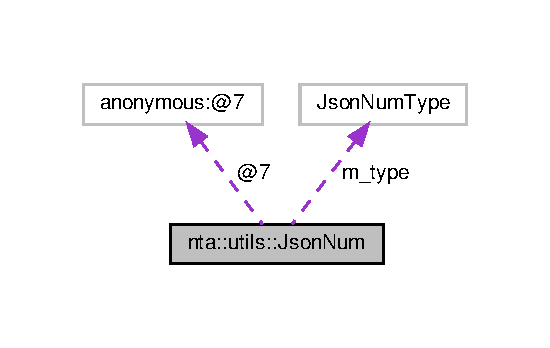
\includegraphics[width=264pt]{d6/d43/classnta_1_1utils_1_1JsonNum__coll__graph}
\end{center}
\end{figure}


\subsection{Member Function Documentation}
\mbox{\Hypertarget{classnta_1_1utils_1_1JsonNum_a89e8033a247c3342d99a762f6110d877}\label{classnta_1_1utils_1_1JsonNum_a89e8033a247c3342d99a762f6110d877}} 
\index{nta\+::utils\+::\+Json\+Num@{nta\+::utils\+::\+Json\+Num}!as\+\_\+uint@{as\+\_\+uint}}
\index{as\+\_\+uint@{as\+\_\+uint}!nta\+::utils\+::\+Json\+Num@{nta\+::utils\+::\+Json\+Num}}
\subsubsection{\texorpdfstring{as\+\_\+uint()}{as\_uint()}}
{\footnotesize\ttfamily uint64\+\_\+t nta\+::utils\+::\+Json\+Num\+::as\+\_\+uint (\begin{DoxyParamCaption}{ }\end{DoxyParamCaption}) const\hspace{0.3cm}{\ttfamily [inline]}}

\begin{DoxyRefDesc}{Todo}
\item[\hyperlink{todo__todo000007}{Todo}]Signal \hyperlink{classnta_1_1ErrorManager}{Error\+Manager} if wrong type \end{DoxyRefDesc}


Definition at line 54 of file json.\+h.



The documentation for this class was generated from the following file\+:\begin{DoxyCompactItemize}
\item 
include/nta/json.\+h\end{DoxyCompactItemize}

\hypertarget{structnta_1_1utils_1_1Json_1_1JsonToken}{}\section{nta\+:\+:utils\+:\+:Json\+:\+:Json\+Token Struct Reference}
\label{structnta_1_1utils_1_1Json_1_1JsonToken}\index{nta\+::utils\+::\+Json\+::\+Json\+Token@{nta\+::utils\+::\+Json\+::\+Json\+Token}}


Used for tokenizing strings before parsing them into \hyperlink{classnta_1_1utils_1_1Json}{Json} objects.  


\subsection*{Public Member Functions}
\begin{DoxyCompactItemize}
\item 
\mbox{\Hypertarget{structnta_1_1utils_1_1Json_1_1JsonToken_a92c89581d01b1bcb9e020455b26d3357}\label{structnta_1_1utils_1_1Json_1_1JsonToken_a92c89581d01b1bcb9e020455b26d3357}} 
{\bfseries Json\+Token} (char c)
\item 
\mbox{\Hypertarget{structnta_1_1utils_1_1Json_1_1JsonToken_af7f642d246c7ed4ef6c8b49505da3ed7}\label{structnta_1_1utils_1_1Json_1_1JsonToken_af7f642d246c7ed4ef6c8b49505da3ed7}} 
{\bfseries Json\+Token} (crstring str)
\item 
\mbox{\Hypertarget{structnta_1_1utils_1_1Json_1_1JsonToken_a4c3b2c9fd0aef1f4b64a50c97044fb16}\label{structnta_1_1utils_1_1Json_1_1JsonToken_a4c3b2c9fd0aef1f4b64a50c97044fb16}} 
{\bfseries Json\+Token} (const \hyperlink{structnta_1_1utils_1_1Json_1_1JsonToken}{Json\+Token} \&other)
\item 
\mbox{\Hypertarget{structnta_1_1utils_1_1Json_1_1JsonToken_abbe6a2f4ad86b45cc89e7f6c1930719f}\label{structnta_1_1utils_1_1Json_1_1JsonToken_abbe6a2f4ad86b45cc89e7f6c1930719f}} 
\hyperlink{structnta_1_1utils_1_1Json_1_1JsonToken}{Json\+Token} \& {\bfseries operator=} (const \hyperlink{structnta_1_1utils_1_1Json_1_1JsonToken}{Json\+Token} \&other)
\item 
\mbox{\Hypertarget{structnta_1_1utils_1_1Json_1_1JsonToken_aaa56bd1310c36cb4a8180079ac9fe627}\label{structnta_1_1utils_1_1Json_1_1JsonToken_aaa56bd1310c36cb4a8180079ac9fe627}} 
bool {\bfseries operator==} (const \hyperlink{structnta_1_1utils_1_1Json_1_1JsonToken}{Json\+Token} \&rhs) const
\item 
\mbox{\Hypertarget{structnta_1_1utils_1_1Json_1_1JsonToken_ae225afc2fbb368fe808b8ed527181a40}\label{structnta_1_1utils_1_1Json_1_1JsonToken_ae225afc2fbb368fe808b8ed527181a40}} 
bool {\bfseries operator!=} (const \hyperlink{structnta_1_1utils_1_1Json_1_1JsonToken}{Json\+Token} \&rhs) const
\end{DoxyCompactItemize}
\subsection*{Public Attributes}
\begin{DoxyCompactItemize}
\item 
\mbox{\Hypertarget{structnta_1_1utils_1_1Json_1_1JsonToken_ab0bf0cda189a3063f326abcbf57532bb}\label{structnta_1_1utils_1_1Json_1_1JsonToken_ab0bf0cda189a3063f326abcbf57532bb}} 
Json\+Token\+Type {\bfseries type}
\item 
\mbox{\Hypertarget{structnta_1_1utils_1_1Json_1_1JsonToken_a7123d444ecb1662248a2b54d4f27d087}\label{structnta_1_1utils_1_1Json_1_1JsonToken_a7123d444ecb1662248a2b54d4f27d087}} 
\begin{tabbing}
xx\=xx\=xx\=xx\=xx\=xx\=xx\=xx\=xx\=\kill
union \{\\
\mbox{\Hypertarget{structnta_1_1utils_1_1Json_1_1JsonToken_a249048bb34d397d9f9034391f07e8666}\label{structnta_1_1utils_1_1Json_1_1JsonToken_a249048bb34d397d9f9034391f07e8666}} 
char $\ast$ {\bfseries str}\\
\mbox{\Hypertarget{structnta_1_1utils_1_1Json_1_1JsonToken_a276868d3bfc600a8e9b00a9719d09122}\label{structnta_1_1utils_1_1Json_1_1JsonToken_a276868d3bfc600a8e9b00a9719d09122}} 
\hyperlink{classnta_1_1utils_1_1JsonNum}{JsonNum} {\bfseries num}\\
\}; \\

\end{tabbing}\end{DoxyCompactItemize}


\subsection{Detailed Description}
Used for tokenizing strings before parsing them into \hyperlink{classnta_1_1utils_1_1Json}{Json} objects. 

Definition at line 225 of file json.\+h.



Collaboration diagram for nta\+:\+:utils\+:\+:Json\+:\+:Json\+Token\+:\nopagebreak
\begin{figure}[H]
\begin{center}
\leavevmode
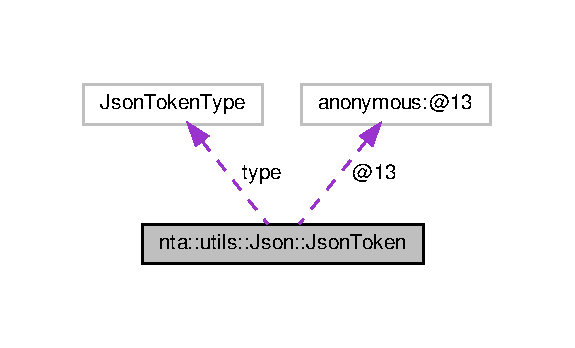
\includegraphics[width=276pt]{d9/d6a/structnta_1_1utils_1_1Json_1_1JsonToken__coll__graph}
\end{center}
\end{figure}


The documentation for this struct was generated from the following file\+:\begin{DoxyCompactItemize}
\item 
include/nta/json.\+h\end{DoxyCompactItemize}

\hypertarget{classnta_1_1Logger}{}\section{nta\+:\+:Logger Class Reference}
\label{classnta_1_1Logger}\index{nta\+::\+Logger@{nta\+::\+Logger}}


stores program information in internal and external logs  




{\ttfamily \#include $<$Logger.\+h$>$}

\subsection*{Static Public Member Functions}
\begin{DoxyCompactItemize}
\item 
\mbox{\Hypertarget{classnta_1_1Logger_a308a3ec22f996556b3d54737ace33543}\label{classnta_1_1Logger_a308a3ec22f996556b3d54737ace33543}} 
static void \hyperlink{classnta_1_1Logger_a308a3ec22f996556b3d54737ace33543}{create\+Log} ()
\begin{DoxyCompactList}\small\item\em creates the log \end{DoxyCompactList}\item 
\mbox{\Hypertarget{classnta_1_1Logger_a71196417598ddd975959924c2ce53c13}\label{classnta_1_1Logger_a71196417598ddd975959924c2ce53c13}} 
static void \hyperlink{classnta_1_1Logger_a71196417598ddd975959924c2ce53c13}{write\+To\+Log} (crstring entry)
\begin{DoxyCompactList}\small\item\em writes an entry in the log \end{DoxyCompactList}\item 
static \hyperlink{structnta_1_1Error}{Error} \hyperlink{classnta_1_1Logger_a22e0cfbb0e04de2c377cdd5297c39eee}{write\+Error\+To\+Log} (crstring error, \hyperlink{namespacenta_a1ddeff35318678e360dfa44ca9577b16}{Error\+Type} type=O\+T\+H\+ER)
\begin{DoxyCompactList}\small\item\em writes entry in log and then exits program \end{DoxyCompactList}\item 
\mbox{\Hypertarget{classnta_1_1Logger_aae8be3709ec3023f987f9b70304cd641}\label{classnta_1_1Logger_aae8be3709ec3023f987f9b70304cd641}} 
static void \hyperlink{classnta_1_1Logger_aae8be3709ec3023f987f9b70304cd641}{indent} (size\+\_\+t tab\+\_\+size=T\+A\+B\+\_\+\+S\+I\+ZE)
\begin{DoxyCompactList}\small\item\em indents entries \end{DoxyCompactList}\item 
\mbox{\Hypertarget{classnta_1_1Logger_a34abdfe89740b8e37461a610f441c8fa}\label{classnta_1_1Logger_a34abdfe89740b8e37461a610f441c8fa}} 
static void \hyperlink{classnta_1_1Logger_a34abdfe89740b8e37461a610f441c8fa}{unindent} (size\+\_\+t tab\+\_\+size=T\+A\+B\+\_\+\+S\+I\+ZE)
\begin{DoxyCompactList}\small\item\em unindents entries \end{DoxyCompactList}\end{DoxyCompactItemize}
\subsection*{Static Private Attributes}
\begin{DoxyCompactItemize}
\item 
\mbox{\Hypertarget{classnta_1_1Logger_aba94cb82e0a5f5dd72719c80de5c3571}\label{classnta_1_1Logger_aba94cb82e0a5f5dd72719c80de5c3571}} 
static std\+::ofstream \hyperlink{classnta_1_1Logger_aba94cb82e0a5f5dd72719c80de5c3571}{m\+\_\+log\+File}
\begin{DoxyCompactList}\small\item\em the file that keeps the external log \end{DoxyCompactList}\item 
\mbox{\Hypertarget{classnta_1_1Logger_a853462b3f8725ff55d36a14220335d72}\label{classnta_1_1Logger_a853462b3f8725ff55d36a14220335d72}} 
static size\+\_\+t {\bfseries m\+\_\+tabs} = 0
\item 
\mbox{\Hypertarget{classnta_1_1Logger_a15106f36caca5fb9554163f3ae47663f}\label{classnta_1_1Logger_a15106f36caca5fb9554163f3ae47663f}} 
static const size\+\_\+t {\bfseries T\+A\+B\+\_\+\+S\+I\+ZE} = 4
\end{DoxyCompactItemize}


\subsection{Detailed Description}
stores program information in internal and external logs 

Definition at line 10 of file Logger.\+h.



Collaboration diagram for nta\+:\+:Logger\+:\nopagebreak
\begin{figure}[H]
\begin{center}
\leavevmode
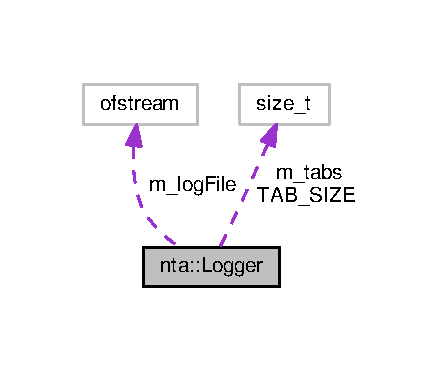
\includegraphics[width=212pt]{d4/d22/classnta_1_1Logger__coll__graph}
\end{center}
\end{figure}


\subsection{Member Function Documentation}
\mbox{\Hypertarget{classnta_1_1Logger_a22e0cfbb0e04de2c377cdd5297c39eee}\label{classnta_1_1Logger_a22e0cfbb0e04de2c377cdd5297c39eee}} 
\index{nta\+::\+Logger@{nta\+::\+Logger}!write\+Error\+To\+Log@{write\+Error\+To\+Log}}
\index{write\+Error\+To\+Log@{write\+Error\+To\+Log}!nta\+::\+Logger@{nta\+::\+Logger}}
\subsubsection{\texorpdfstring{write\+Error\+To\+Log()}{writeErrorToLog()}}
{\footnotesize\ttfamily \hyperlink{structnta_1_1Error}{Error} nta\+::\+Logger\+::write\+Error\+To\+Log (\begin{DoxyParamCaption}\item[{crstring}]{error,  }\item[{\hyperlink{namespacenta_a1ddeff35318678e360dfa44ca9577b16}{Error\+Type}}]{type = {\ttfamily OTHER} }\end{DoxyParamCaption})\hspace{0.3cm}{\ttfamily [static]}}



writes entry in log and then exits program 

\begin{DoxyRefDesc}{Todo}
\item[\hyperlink{todo__todo000026}{Todo}]Make sure all the code that previously assumed this function always exits still behaves sensibly \end{DoxyRefDesc}


Definition at line 23 of file Logger.\+cpp.



Referenced by nta\+::\+G\+L\+S\+L\+Program\+::compile\+Shader(), nta\+::\+Window\+::create\+Window(), nta\+::\+Audio\+Manager\+::get\+Sound\+Effect(), nta\+::\+Resource\+Manager\+::get\+Texture(), nta\+::\+G\+L\+S\+L\+Program\+::get\+Uniform\+Location(), nta\+::init(), nta\+::\+Audio\+Manager\+::init(), nta\+::\+G\+L\+S\+L\+Program\+::link\+Shaders(), nta\+::\+I\+O\+Manager\+::read\+File\+To\+Buffer(), nta\+::\+Image\+Loader\+::read\+Image(), and nta\+::\+Sprite\+Font\+::\+Sprite\+Font().

Here is the call graph for this function\+:\nopagebreak
\begin{figure}[H]
\begin{center}
\leavevmode
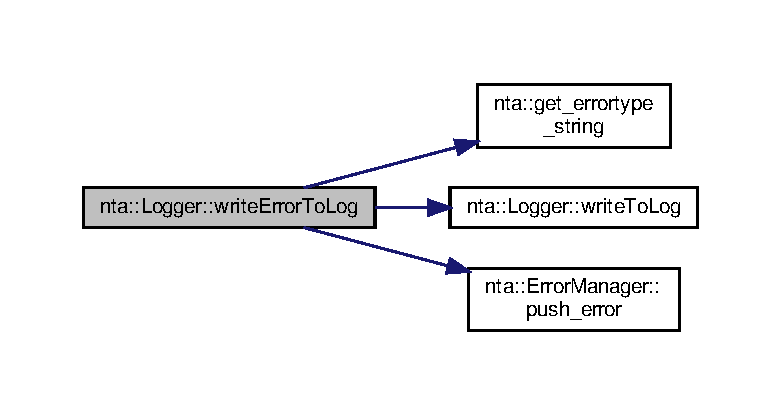
\includegraphics[width=350pt]{d6/d0d/classnta_1_1Logger_a22e0cfbb0e04de2c377cdd5297c39eee_cgraph}
\end{center}
\end{figure}
Here is the caller graph for this function\+:\nopagebreak
\begin{figure}[H]
\begin{center}
\leavevmode
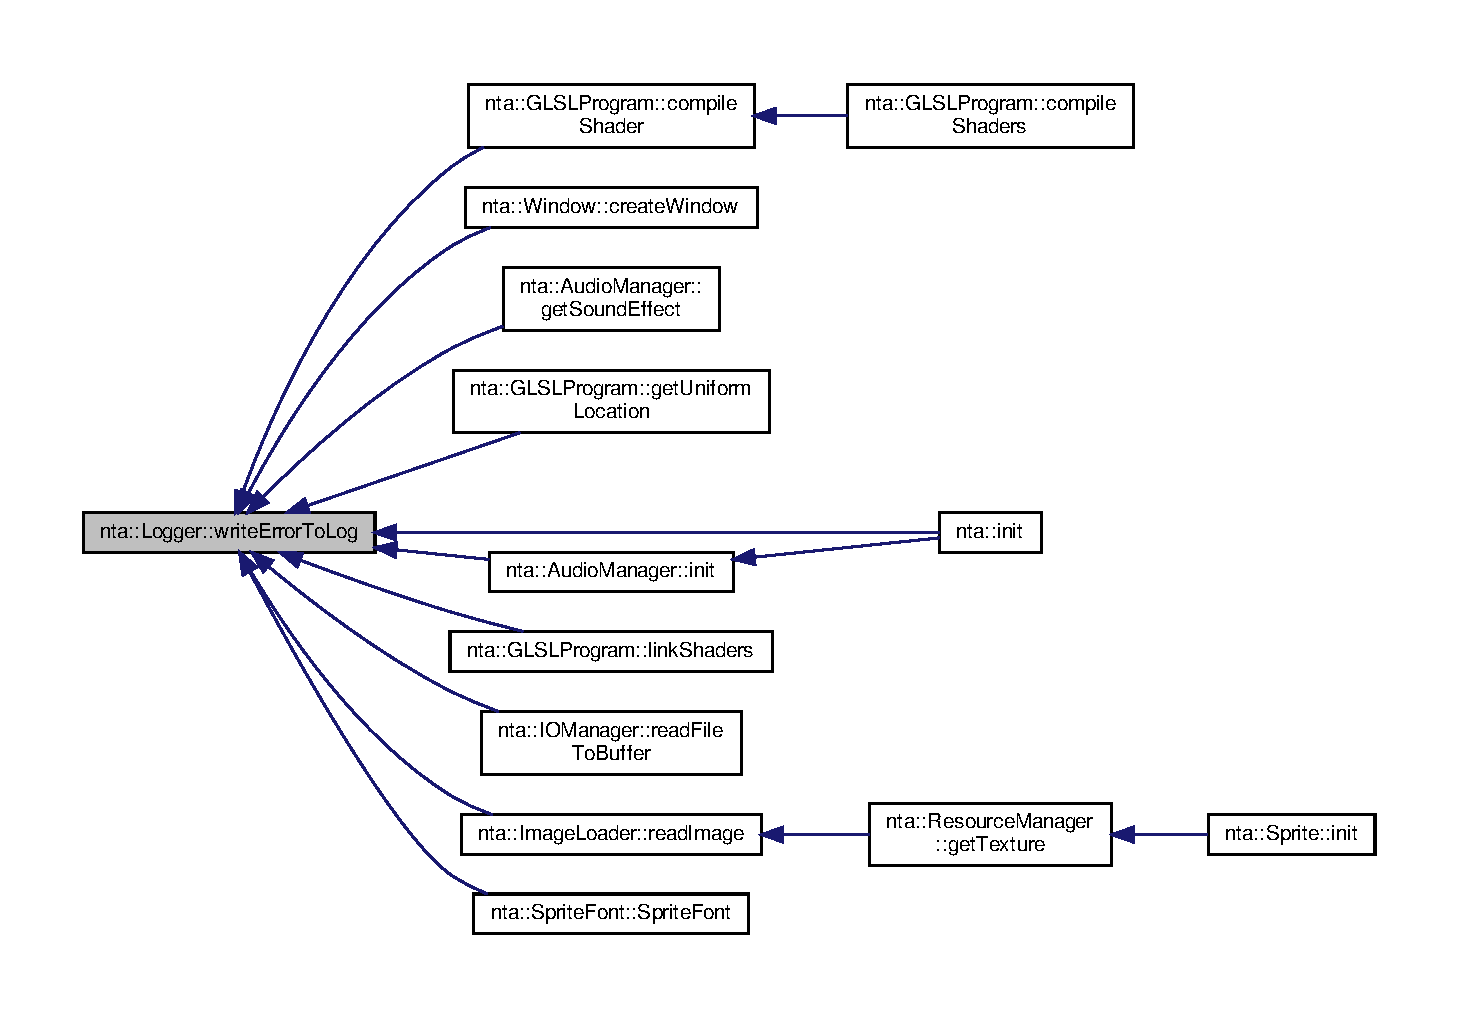
\includegraphics[width=350pt]{d6/d0d/classnta_1_1Logger_a22e0cfbb0e04de2c377cdd5297c39eee_icgraph}
\end{center}
\end{figure}


The documentation for this class was generated from the following files\+:\begin{DoxyCompactItemize}
\item 
include/nta/Logger.\+h\item 
src/Logger.\+cpp\end{DoxyCompactItemize}

\hypertarget{classnta_1_1Music}{}\section{nta\+:\+:Music Class Reference}
\label{classnta_1_1Music}\index{nta\+::\+Music@{nta\+::\+Music}}


Represents a longer piece of music.  




{\ttfamily \#include $<$Audio\+Manager.\+h$>$}

\subsection*{Public Member Functions}
\begin{DoxyCompactItemize}
\item 
\mbox{\Hypertarget{classnta_1_1Music_a2987f4f84b0c0a0094967821a7b14f64}\label{classnta_1_1Music_a2987f4f84b0c0a0094967821a7b14f64}} 
void \hyperlink{classnta_1_1Music_a2987f4f84b0c0a0094967821a7b14f64}{play} (int num\+Loops=1) const
\begin{DoxyCompactList}\small\item\em plays music \end{DoxyCompactList}\item 
\mbox{\Hypertarget{classnta_1_1Music_a8382cffd123f37f3f1426a0d461e9541}\label{classnta_1_1Music_a8382cffd123f37f3f1426a0d461e9541}} 
void \hyperlink{classnta_1_1Music_a8382cffd123f37f3f1426a0d461e9541}{pause} () const
\begin{DoxyCompactList}\small\item\em pauses music (can be resumed) \end{DoxyCompactList}\item 
\mbox{\Hypertarget{classnta_1_1Music_ade2d11ebc9273494b344e089cd7b58b8}\label{classnta_1_1Music_ade2d11ebc9273494b344e089cd7b58b8}} 
void \hyperlink{classnta_1_1Music_ade2d11ebc9273494b344e089cd7b58b8}{stop} () const
\begin{DoxyCompactList}\small\item\em stops music (must be replayed from beginning) \end{DoxyCompactList}\item 
\mbox{\Hypertarget{classnta_1_1Music_a7eb8159db905f34ebf6ad48ec9a1afa1}\label{classnta_1_1Music_a7eb8159db905f34ebf6ad48ec9a1afa1}} 
void \hyperlink{classnta_1_1Music_a7eb8159db905f34ebf6ad48ec9a1afa1}{resume} () const
\begin{DoxyCompactList}\small\item\em resumes paused music \end{DoxyCompactList}\end{DoxyCompactItemize}
\subsection*{Private Member Functions}
\begin{DoxyCompactItemize}
\item 
\mbox{\Hypertarget{classnta_1_1Music_aa38f19729b8afd2591d236dde3c65edd}\label{classnta_1_1Music_aa38f19729b8afd2591d236dde3c65edd}} 
\hyperlink{classnta_1_1Music_aa38f19729b8afd2591d236dde3c65edd}{Music} (Mix\+\_\+\+Music $\ast$m)
\begin{DoxyCompactList}\small\item\em constructor simply stores music \end{DoxyCompactList}\item 
\mbox{\Hypertarget{classnta_1_1Music_a5cb0a3bbc5222752b0cbc9a90468e98b}\label{classnta_1_1Music_a5cb0a3bbc5222752b0cbc9a90468e98b}} 
\hyperlink{classnta_1_1Music_a5cb0a3bbc5222752b0cbc9a90468e98b}{$\sim$\+Music} ()
\begin{DoxyCompactList}\small\item\em destructor frees stored music \end{DoxyCompactList}\end{DoxyCompactItemize}
\subsection*{Private Attributes}
\begin{DoxyCompactItemize}
\item 
\mbox{\Hypertarget{classnta_1_1Music_a8a39359bb2dc8d8d350119ee47a7c3a0}\label{classnta_1_1Music_a8a39359bb2dc8d8d350119ee47a7c3a0}} 
Mix\+\_\+\+Music $\ast$ \hyperlink{classnta_1_1Music_a8a39359bb2dc8d8d350119ee47a7c3a0}{m\+\_\+music} = nullptr
\begin{DoxyCompactList}\small\item\em the stored music \end{DoxyCompactList}\end{DoxyCompactItemize}
\subsection*{Friends}
\begin{DoxyCompactItemize}
\item 
\mbox{\Hypertarget{classnta_1_1Music_a85edaa7e5c3ae68dabadd5373890591e}\label{classnta_1_1Music_a85edaa7e5c3ae68dabadd5373890591e}} 
class {\bfseries Audio\+Manager}
\end{DoxyCompactItemize}


\subsection{Detailed Description}
Represents a longer piece of music. 

Definition at line 33 of file Audio\+Manager.\+h.



The documentation for this class was generated from the following file\+:\begin{DoxyCompactItemize}
\item 
include/nta/Audio\+Manager.\+h\end{DoxyCompactItemize}

\hypertarget{structnta_1_1Particle2D}{}\section{nta\+:\+:Particle2D Struct Reference}
\label{structnta_1_1Particle2D}\index{nta\+::\+Particle2D@{nta\+::\+Particle2D}}


Represents a simple 2d particle.  




{\ttfamily \#include $<$Particle\+Batch2\+D.\+h$>$}

\subsection*{Public Member Functions}
\begin{DoxyCompactItemize}
\item 
\mbox{\Hypertarget{structnta_1_1Particle2D_abfe29bfc0b8719eeb17df8268368ce52}\label{structnta_1_1Particle2D_abfe29bfc0b8719eeb17df8268368ce52}} 
{\bfseries Particle2D} (crvec2 c, crvec2 v, crvec4 col)
\end{DoxyCompactItemize}
\subsection*{Public Attributes}
\begin{DoxyCompactItemize}
\item 
\mbox{\Hypertarget{structnta_1_1Particle2D_a47ae411f47152a2b064dc216692302be}\label{structnta_1_1Particle2D_a47ae411f47152a2b064dc216692302be}} 
glm\+::vec2 {\bfseries center}
\item 
\mbox{\Hypertarget{structnta_1_1Particle2D_a7194c7ec065b7221ed61c861595cabb5}\label{structnta_1_1Particle2D_a7194c7ec065b7221ed61c861595cabb5}} 
glm\+::vec2 {\bfseries velocity}
\item 
\mbox{\Hypertarget{structnta_1_1Particle2D_a3d3233a4de4f2c2b46715dd9a7187994}\label{structnta_1_1Particle2D_a3d3233a4de4f2c2b46715dd9a7187994}} 
glm\+::vec4 {\bfseries color}
\item 
\mbox{\Hypertarget{structnta_1_1Particle2D_acfae159a4e2072f7896fac058e11e66f}\label{structnta_1_1Particle2D_acfae159a4e2072f7896fac058e11e66f}} 
float {\bfseries life}
\end{DoxyCompactItemize}


\subsection{Detailed Description}
Represents a simple 2d particle. 

Definition at line 10 of file Particle\+Batch2\+D.\+h.



Collaboration diagram for nta\+:\+:Particle2D\+:\nopagebreak
\begin{figure}[H]
\begin{center}
\leavevmode
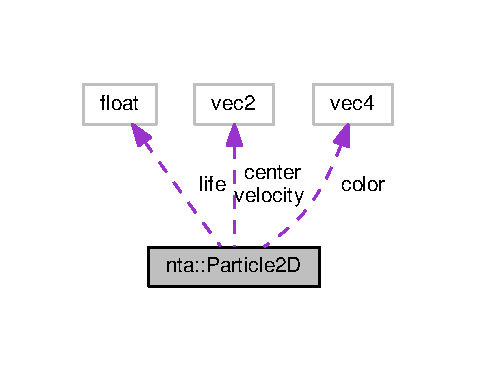
\includegraphics[width=229pt]{df/d87/structnta_1_1Particle2D__coll__graph}
\end{center}
\end{figure}


The documentation for this struct was generated from the following file\+:\begin{DoxyCompactItemize}
\item 
include/nta/Particle\+Batch2\+D.\+h\end{DoxyCompactItemize}

\hypertarget{classnta_1_1ParticleBatch2D}{}\section{nta\+:\+:Particle\+Batch2D Class Reference}
\label{classnta_1_1ParticleBatch2D}\index{nta\+::\+Particle\+Batch2D@{nta\+::\+Particle\+Batch2D}}


Represents a batch of particles of the same \char`\"{}type\char`\"{}.  




{\ttfamily \#include $<$Particle\+Batch2\+D.\+h$>$}

\subsection*{Public Member Functions}
\begin{DoxyCompactItemize}
\item 
\mbox{\Hypertarget{classnta_1_1ParticleBatch2D_af81efd4598cd578c2eddbcab6b5d3f5d}\label{classnta_1_1ParticleBatch2D_af81efd4598cd578c2eddbcab6b5d3f5d}} 
\hyperlink{classnta_1_1ParticleBatch2D_af81efd4598cd578c2eddbcab6b5d3f5d}{Particle\+Batch2D} ()
\begin{DoxyCompactList}\small\item\em basic constructor \end{DoxyCompactList}\item 
\mbox{\Hypertarget{classnta_1_1ParticleBatch2D_ac21b6437fdd8e746c6fce095b4dbc03a}\label{classnta_1_1ParticleBatch2D_ac21b6437fdd8e746c6fce095b4dbc03a}} 
\hyperlink{classnta_1_1ParticleBatch2D_ac21b6437fdd8e746c6fce095b4dbc03a}{$\sim$\+Particle\+Batch2D} ()
\begin{DoxyCompactList}\small\item\em deletes particles \end{DoxyCompactList}\item 
\mbox{\Hypertarget{classnta_1_1ParticleBatch2D_a328f04a39eb9baa821ad95b2f455a7b0}\label{classnta_1_1ParticleBatch2D_a328f04a39eb9baa821ad95b2f455a7b0}} 
void \hyperlink{classnta_1_1ParticleBatch2D_a328f04a39eb9baa821ad95b2f455a7b0}{init} (float il, float dr, float r, int mp, int tex, std\+::function$<$ void(\hyperlink{structnta_1_1Particle2D}{Particle2D} \&, float)$>$ update\+Func)
\begin{DoxyCompactList}\small\item\em initializes particle batch by specifying properties \end{DoxyCompactList}\item 
\mbox{\Hypertarget{classnta_1_1ParticleBatch2D_aeb80340cf60145569e7d30e5e25fd9c0}\label{classnta_1_1ParticleBatch2D_aeb80340cf60145569e7d30e5e25fd9c0}} 
void \hyperlink{classnta_1_1ParticleBatch2D_aeb80340cf60145569e7d30e5e25fd9c0}{add\+Particle} (\hyperlink{structnta_1_1Particle2D}{Particle2D} p)
\begin{DoxyCompactList}\small\item\em adds a particle to the batch \end{DoxyCompactList}\item 
\mbox{\Hypertarget{classnta_1_1ParticleBatch2D_a270e573b2a767bf32fde34d17d838e69}\label{classnta_1_1ParticleBatch2D_a270e573b2a767bf32fde34d17d838e69}} 
void \hyperlink{classnta_1_1ParticleBatch2D_a270e573b2a767bf32fde34d17d838e69}{draw} (\hyperlink{classnta_1_1SpriteBatch}{Sprite\+Batch} \&batch) const
\begin{DoxyCompactList}\small\item\em draws all the particles \end{DoxyCompactList}\item 
\mbox{\Hypertarget{classnta_1_1ParticleBatch2D_a55d3f2b663039bb95e847f0770c864cf}\label{classnta_1_1ParticleBatch2D_a55d3f2b663039bb95e847f0770c864cf}} 
void \hyperlink{classnta_1_1ParticleBatch2D_a55d3f2b663039bb95e847f0770c864cf}{update} (float dt)
\begin{DoxyCompactList}\small\item\em updates the particles \end{DoxyCompactList}\item 
\mbox{\Hypertarget{classnta_1_1ParticleBatch2D_a1046b22d239222435e74011b3683a5c6}\label{classnta_1_1ParticleBatch2D_a1046b22d239222435e74011b3683a5c6}} 
void \hyperlink{classnta_1_1ParticleBatch2D_a1046b22d239222435e74011b3683a5c6}{clear} ()
\begin{DoxyCompactList}\small\item\em removes all particles \end{DoxyCompactList}\end{DoxyCompactItemize}
\subsection*{Private Member Functions}
\begin{DoxyCompactItemize}
\item 
\mbox{\Hypertarget{classnta_1_1ParticleBatch2D_a123aac9af29133bfe358b9895de2b2ce}\label{classnta_1_1ParticleBatch2D_a123aac9af29133bfe358b9895de2b2ce}} 
int \hyperlink{classnta_1_1ParticleBatch2D_a123aac9af29133bfe358b9895de2b2ce}{get\+Free\+Particle} () const
\begin{DoxyCompactList}\small\item\em returns index of particle with the minimum life \end{DoxyCompactList}\end{DoxyCompactItemize}
\subsection*{Private Attributes}
\begin{DoxyCompactItemize}
\item 
\mbox{\Hypertarget{classnta_1_1ParticleBatch2D_abfe8d182f35c8eb0f882902d292129be}\label{classnta_1_1ParticleBatch2D_abfe8d182f35c8eb0f882902d292129be}} 
std\+::function$<$ void(\hyperlink{structnta_1_1Particle2D}{Particle2D} \&, float)$>$ \hyperlink{classnta_1_1ParticleBatch2D_abfe8d182f35c8eb0f882902d292129be}{m\+\_\+update\+Function}
\begin{DoxyCompactList}\small\item\em the function used to update the particles \end{DoxyCompactList}\item 
\mbox{\Hypertarget{classnta_1_1ParticleBatch2D_ad410f47c5312b018125795882db9aa6c}\label{classnta_1_1ParticleBatch2D_ad410f47c5312b018125795882db9aa6c}} 
\hyperlink{structnta_1_1Particle2D}{Particle2D} $\ast$ \hyperlink{classnta_1_1ParticleBatch2D_ad410f47c5312b018125795882db9aa6c}{m\+\_\+particles} = nullptr
\begin{DoxyCompactList}\small\item\em the particles themselves \end{DoxyCompactList}\item 
\mbox{\Hypertarget{classnta_1_1ParticleBatch2D_a9c789bf8a6449ed7db554cee6f3c918e}\label{classnta_1_1ParticleBatch2D_a9c789bf8a6449ed7db554cee6f3c918e}} 
float \hyperlink{classnta_1_1ParticleBatch2D_a9c789bf8a6449ed7db554cee6f3c918e}{m\+\_\+initial\+Life}
\begin{DoxyCompactList}\small\item\em the life every particle starts out with \end{DoxyCompactList}\item 
\mbox{\Hypertarget{classnta_1_1ParticleBatch2D_a59d0ca59a6f1c83d7a2c7c210e87bcc1}\label{classnta_1_1ParticleBatch2D_a59d0ca59a6f1c83d7a2c7c210e87bcc1}} 
float \hyperlink{classnta_1_1ParticleBatch2D_a59d0ca59a6f1c83d7a2c7c210e87bcc1}{m\+\_\+decay\+Rate}
\begin{DoxyCompactList}\small\item\em the rate with which particles lose life \end{DoxyCompactList}\item 
\mbox{\Hypertarget{classnta_1_1ParticleBatch2D_ac564b88da2f73d5692cbdec15478fe4d}\label{classnta_1_1ParticleBatch2D_ac564b88da2f73d5692cbdec15478fe4d}} 
float \hyperlink{classnta_1_1ParticleBatch2D_ac564b88da2f73d5692cbdec15478fe4d}{m\+\_\+radius}
\begin{DoxyCompactList}\small\item\em the radius of an individual particle \end{DoxyCompactList}\item 
\mbox{\Hypertarget{classnta_1_1ParticleBatch2D_acf0dbc3bae31f962ed403daf06848948}\label{classnta_1_1ParticleBatch2D_acf0dbc3bae31f962ed403daf06848948}} 
int \hyperlink{classnta_1_1ParticleBatch2D_acf0dbc3bae31f962ed403daf06848948}{m\+\_\+max\+Particles}
\begin{DoxyCompactList}\small\item\em maximum number of particles allowed \end{DoxyCompactList}\item 
\mbox{\Hypertarget{classnta_1_1ParticleBatch2D_a73232a0481db52884b42c50deb456add}\label{classnta_1_1ParticleBatch2D_a73232a0481db52884b42c50deb456add}} 
int \hyperlink{classnta_1_1ParticleBatch2D_a73232a0481db52884b42c50deb456add}{m\+\_\+texture\+ID}
\begin{DoxyCompactList}\small\item\em texture used by the particles \end{DoxyCompactList}\end{DoxyCompactItemize}


\subsection{Detailed Description}
Represents a batch of particles of the same \char`\"{}type\char`\"{}. 

Definition at line 21 of file Particle\+Batch2\+D.\+h.



Collaboration diagram for nta\+:\+:Particle\+Batch2D\+:
\nopagebreak
\begin{figure}[H]
\begin{center}
\leavevmode
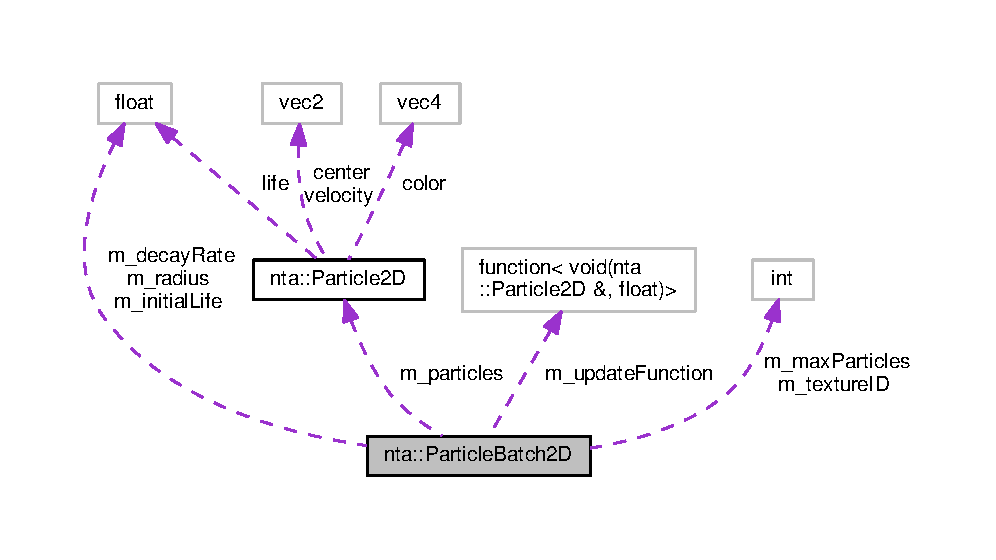
\includegraphics[width=350pt]{d4/d22/classnta_1_1ParticleBatch2D__coll__graph}
\end{center}
\end{figure}


The documentation for this class was generated from the following files\+:\begin{DoxyCompactItemize}
\item 
include/nta/Particle\+Batch2\+D.\+h\item 
src/Particle\+Batch2\+D.\+cpp\end{DoxyCompactItemize}

\hypertarget{classnta_1_1ParticleEngine2D}{}\section{nta\+:\+:Particle\+Engine2D Class Reference}
\label{classnta_1_1ParticleEngine2D}\index{nta\+::\+Particle\+Engine2D@{nta\+::\+Particle\+Engine2D}}


Responsible for handling multiple particle batches.  




{\ttfamily \#include $<$Particle\+Engine2\+D.\+h$>$}

\subsection*{Public Member Functions}
\begin{DoxyCompactItemize}
\item 
\mbox{\Hypertarget{classnta_1_1ParticleEngine2D_a0fdd494f4e47d56ac2cee6306e682c0f}\label{classnta_1_1ParticleEngine2D_a0fdd494f4e47d56ac2cee6306e682c0f}} 
\hyperlink{classnta_1_1ParticleEngine2D_a0fdd494f4e47d56ac2cee6306e682c0f}{Particle\+Engine2D} ()
\begin{DoxyCompactList}\small\item\em basic constructor \end{DoxyCompactList}\item 
\mbox{\Hypertarget{classnta_1_1ParticleEngine2D_a9819d90a1852b474bb3014a8c8d506a1}\label{classnta_1_1ParticleEngine2D_a9819d90a1852b474bb3014a8c8d506a1}} 
\hyperlink{classnta_1_1ParticleEngine2D_a9819d90a1852b474bb3014a8c8d506a1}{$\sim$\+Particle\+Engine2D} ()
\begin{DoxyCompactList}\small\item\em deletes batches \end{DoxyCompactList}\item 
\mbox{\Hypertarget{classnta_1_1ParticleEngine2D_a1543908144e9aeb9ae1b7529e82c0ad7}\label{classnta_1_1ParticleEngine2D_a1543908144e9aeb9ae1b7529e82c0ad7}} 
void \hyperlink{classnta_1_1ParticleEngine2D_a1543908144e9aeb9ae1b7529e82c0ad7}{add\+Batch} (\hyperlink{classnta_1_1ParticleBatch2D}{Particle\+Batch2D} $\ast$batch)
\begin{DoxyCompactList}\small\item\em adds a batch \end{DoxyCompactList}\item 
\mbox{\Hypertarget{classnta_1_1ParticleEngine2D_a759937cf45e74162ce85269ddf59237b}\label{classnta_1_1ParticleEngine2D_a759937cf45e74162ce85269ddf59237b}} 
void \hyperlink{classnta_1_1ParticleEngine2D_a759937cf45e74162ce85269ddf59237b}{draw} (\hyperlink{classnta_1_1SpriteBatch}{Sprite\+Batch} \&batch) const
\begin{DoxyCompactList}\small\item\em renders all batches \end{DoxyCompactList}\item 
\mbox{\Hypertarget{classnta_1_1ParticleEngine2D_ad9c7f1be65505d86c23f5754e5fd9430}\label{classnta_1_1ParticleEngine2D_ad9c7f1be65505d86c23f5754e5fd9430}} 
void \hyperlink{classnta_1_1ParticleEngine2D_ad9c7f1be65505d86c23f5754e5fd9430}{update} (float dt) const
\begin{DoxyCompactList}\small\item\em updates all batches \end{DoxyCompactList}\end{DoxyCompactItemize}
\subsection*{Private Attributes}
\begin{DoxyCompactItemize}
\item 
\mbox{\Hypertarget{classnta_1_1ParticleEngine2D_a7d928b070dbc09e68d13fd7f9d087549}\label{classnta_1_1ParticleEngine2D_a7d928b070dbc09e68d13fd7f9d087549}} 
std\+::vector$<$ \hyperlink{classnta_1_1ParticleBatch2D}{Particle\+Batch2D} $\ast$ $>$ \hyperlink{classnta_1_1ParticleEngine2D_a7d928b070dbc09e68d13fd7f9d087549}{m\+\_\+batches}
\begin{DoxyCompactList}\small\item\em the particle batches \end{DoxyCompactList}\end{DoxyCompactItemize}


\subsection{Detailed Description}
Responsible for handling multiple particle batches. 

Definition at line 10 of file Particle\+Engine2\+D.\+h.



Collaboration diagram for nta\+:\+:Particle\+Engine2D\+:\nopagebreak
\begin{figure}[H]
\begin{center}
\leavevmode
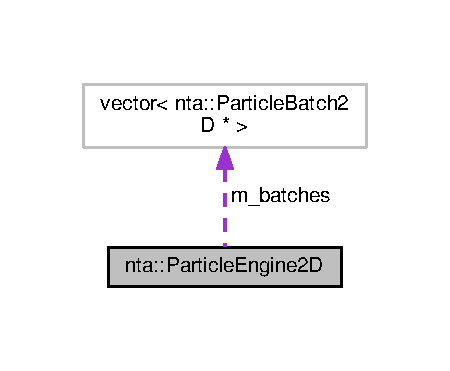
\includegraphics[width=216pt]{db/dbd/classnta_1_1ParticleEngine2D__coll__graph}
\end{center}
\end{figure}


The documentation for this class was generated from the following files\+:\begin{DoxyCompactItemize}
\item 
include/nta/Particle\+Engine2\+D.\+h\item 
src/Particle\+Engine2\+D.\+cpp\end{DoxyCompactItemize}

\hypertarget{structnta_1_1Primitive}{}\section{nta\+:\+:Primitive Struct Reference}
\label{structnta_1_1Primitive}\index{nta\+::\+Primitive@{nta\+::\+Primitive}}


represents a primitive (point, line, triangle, etc.)  




{\ttfamily \#include $<$Primitive\+Batch.\+h$>$}

\subsection*{Public Member Functions}
\begin{DoxyCompactItemize}
\item 
\mbox{\Hypertarget{structnta_1_1Primitive_ad8eb45115ed7647d71360ce6366eb2bc}\label{structnta_1_1Primitive_ad8eb45115ed7647d71360ce6366eb2bc}} 
\hyperlink{structnta_1_1Primitive_ad8eb45115ed7647d71360ce6366eb2bc}{Primitive} (const std\+::initializer\+\_\+list$<$ \hyperlink{structnta_1_1Vertex2D}{Vertex2D} $>$ \&verts, G\+Luint tex\+ID, float d)
\begin{DoxyCompactList}\small\item\em Constructs a primitive from a list of vertices. \end{DoxyCompactList}\item 
\mbox{\Hypertarget{structnta_1_1Primitive_aa0325b0eb7dc6ec40294b9e47feb750b}\label{structnta_1_1Primitive_aa0325b0eb7dc6ec40294b9e47feb750b}} 
{\footnotesize template$<$class Iterator $>$ }\\{\bfseries Primitive} (Iterator first, Iterator last, G\+Luint tex\+ID, float d)
\item 
\mbox{\Hypertarget{structnta_1_1Primitive_a6f5cc606b1b9e6537daa5f9413912416}\label{structnta_1_1Primitive_a6f5cc606b1b9e6537daa5f9413912416}} 
\hyperlink{structnta_1_1Primitive_a6f5cc606b1b9e6537daa5f9413912416}{Primitive} (std\+::size\+\_\+t num\+Sides, crvec2 center, float side\+Length, crvec4 color, float d)
\begin{DoxyCompactList}\small\item\em Constructs an untextured regular polygon. \end{DoxyCompactList}\item 
\mbox{\Hypertarget{structnta_1_1Primitive_a39fbab541466b58744a8c7a0aa4eb49c}\label{structnta_1_1Primitive_a39fbab541466b58744a8c7a0aa4eb49c}} 
\hyperlink{structnta_1_1Primitive_a39fbab541466b58744a8c7a0aa4eb49c}{$\sim$\+Primitive} ()
\begin{DoxyCompactList}\small\item\em destructor \end{DoxyCompactList}\end{DoxyCompactItemize}
\subsection*{Public Attributes}
\begin{DoxyCompactItemize}
\item 
\mbox{\Hypertarget{structnta_1_1Primitive_a4443e427fb512898693bba61a8ac4654}\label{structnta_1_1Primitive_a4443e427fb512898693bba61a8ac4654}} 
float \hyperlink{structnta_1_1Primitive_a4443e427fb512898693bba61a8ac4654}{depth}
\begin{DoxyCompactList}\small\item\em the depth of the primitive \end{DoxyCompactList}\item 
\mbox{\Hypertarget{structnta_1_1Primitive_a203f519bb8fefeaae5253ef3739b7701}\label{structnta_1_1Primitive_a203f519bb8fefeaae5253ef3739b7701}} 
G\+Luint \hyperlink{structnta_1_1Primitive_a203f519bb8fefeaae5253ef3739b7701}{texture\+ID}
\begin{DoxyCompactList}\small\item\em the texture used by the primitive \end{DoxyCompactList}\item 
\mbox{\Hypertarget{structnta_1_1Primitive_a4fbc49e3dcd593551b6e65e59d842687}\label{structnta_1_1Primitive_a4fbc49e3dcd593551b6e65e59d842687}} 
std\+::vector$<$ \hyperlink{structnta_1_1Vertex2D}{Vertex2D} $>$ \hyperlink{structnta_1_1Primitive_a4fbc49e3dcd593551b6e65e59d842687}{vertices}
\begin{DoxyCompactList}\small\item\em the vertices that make up the primitive \end{DoxyCompactList}\end{DoxyCompactItemize}


\subsection{Detailed Description}
represents a primitive (point, line, triangle, etc.) 

Definition at line 8 of file Primitive\+Batch.\+h.



The documentation for this struct was generated from the following file\+:\begin{DoxyCompactItemize}
\item 
include/nta/Primitive\+Batch.\+h\end{DoxyCompactItemize}

\hypertarget{classnta_1_1PrimitiveBatch}{}\section{nta\+:\+:Primitive\+Batch Class Reference}
\label{classnta_1_1PrimitiveBatch}\index{nta\+::\+Primitive\+Batch@{nta\+::\+Primitive\+Batch}}


represents a collection of primitives to be drawn  




{\ttfamily \#include $<$Primitive\+Batch.\+h$>$}

\subsection*{Public Member Functions}
\begin{DoxyCompactItemize}
\item 
\mbox{\Hypertarget{classnta_1_1PrimitiveBatch_a28628a90db31796dd0d1cf770dbe9ff5}\label{classnta_1_1PrimitiveBatch_a28628a90db31796dd0d1cf770dbe9ff5}} 
\hyperlink{classnta_1_1PrimitiveBatch_a28628a90db31796dd0d1cf770dbe9ff5}{Primitive\+Batch} ()
\begin{DoxyCompactList}\small\item\em constructor and destructor \end{DoxyCompactList}\item 
\mbox{\Hypertarget{classnta_1_1PrimitiveBatch_a3cf74d5aaf9e56b0d98512ba8b94d01f}\label{classnta_1_1PrimitiveBatch_a3cf74d5aaf9e56b0d98512ba8b94d01f}} 
int \hyperlink{classnta_1_1PrimitiveBatch_a3cf74d5aaf9e56b0d98512ba8b94d01f}{num\+Primitives} () const
\begin{DoxyCompactList}\small\item\em returns number of primitives to be rendered \end{DoxyCompactList}\item 
\mbox{\Hypertarget{classnta_1_1PrimitiveBatch_a425c70802333e18a6cd019aec145f07b}\label{classnta_1_1PrimitiveBatch_a425c70802333e18a6cd019aec145f07b}} 
void \hyperlink{classnta_1_1PrimitiveBatch_a425c70802333e18a6cd019aec145f07b}{init} ()
\begin{DoxyCompactList}\small\item\em initializes the batch \end{DoxyCompactList}\item 
\mbox{\Hypertarget{classnta_1_1PrimitiveBatch_a589f1ebad11f83187f2ce8f81875fe22}\label{classnta_1_1PrimitiveBatch_a589f1ebad11f83187f2ce8f81875fe22}} 
void \hyperlink{classnta_1_1PrimitiveBatch_a589f1ebad11f83187f2ce8f81875fe22}{begin} ()
\begin{DoxyCompactList}\small\item\em begins collection of primitive \end{DoxyCompactList}\item 
\mbox{\Hypertarget{classnta_1_1PrimitiveBatch_a570927ae1e495ff444d44bd6d19c74ff}\label{classnta_1_1PrimitiveBatch_a570927ae1e495ff444d44bd6d19c74ff}} 
void \hyperlink{classnta_1_1PrimitiveBatch_a570927ae1e495ff444d44bd6d19c74ff}{end} ()
\begin{DoxyCompactList}\small\item\em ends collection of primitive and prepares for rendering \end{DoxyCompactList}\item 
\mbox{\Hypertarget{classnta_1_1PrimitiveBatch_a61a1fd06003233eac050ea7317fafc43}\label{classnta_1_1PrimitiveBatch_a61a1fd06003233eac050ea7317fafc43}} 
void \hyperlink{classnta_1_1PrimitiveBatch_a61a1fd06003233eac050ea7317fafc43}{add\+Primitive} (\hyperlink{structnta_1_1Primitive}{Primitive} $\ast$primitive)
\begin{DoxyCompactList}\small\item\em adds a primitive to the batch \end{DoxyCompactList}\item 
\mbox{\Hypertarget{classnta_1_1PrimitiveBatch_a3e27ba0adbccc7d83254ea1877025d05}\label{classnta_1_1PrimitiveBatch_a3e27ba0adbccc7d83254ea1877025d05}} 
void {\bfseries add\+Primitive} (const std\+::initializer\+\_\+list$<$ \hyperlink{structnta_1_1Vertex2D}{Vertex2D} $>$ \&vertices, G\+Luint texture\+ID=-\/1, float depth=N\+T\+A\+\_\+\+D\+E\+F\+A\+U\+L\+T\+\_\+\+D\+E\+P\+TH)
\item 
\mbox{\Hypertarget{classnta_1_1PrimitiveBatch_a632c197f0f3362d52ce8c0ff1e03745c}\label{classnta_1_1PrimitiveBatch_a632c197f0f3362d52ce8c0ff1e03745c}} 
{\footnotesize template$<$class Iterator $>$ }\\void {\bfseries add\+Primitive} (Iterator first, Iterator last, G\+Luint texture\+ID=-\/1, float depth=N\+T\+A\+\_\+\+D\+E\+F\+A\+U\+L\+T\+\_\+\+D\+E\+P\+TH)
\item 
\mbox{\Hypertarget{classnta_1_1PrimitiveBatch_ac66007384a7932b1082c5d9baab8d836}\label{classnta_1_1PrimitiveBatch_ac66007384a7932b1082c5d9baab8d836}} 
void {\bfseries add\+Primitive} (std\+::size\+\_\+t num\+Sides, crvec2 center=glm\+::vec2(0), float side\+Length=1.\+0, crvec4 color=glm\+::vec4(1), float orientation=0., float depth=N\+T\+A\+\_\+\+D\+E\+F\+A\+U\+L\+T\+\_\+\+D\+E\+P\+TH)
\item 
\mbox{\Hypertarget{classnta_1_1PrimitiveBatch_a899411db2d7abc313d8bef4a19fd097e}\label{classnta_1_1PrimitiveBatch_a899411db2d7abc313d8bef4a19fd097e}} 
void \hyperlink{classnta_1_1PrimitiveBatch_a899411db2d7abc313d8bef4a19fd097e}{render} () const
\begin{DoxyCompactList}\small\item\em renders the primitives \end{DoxyCompactList}\end{DoxyCompactItemize}
\subsection*{Private Member Functions}
\begin{DoxyCompactItemize}
\item 
\mbox{\Hypertarget{classnta_1_1PrimitiveBatch_a1968cc783eb6ce57dec923a7d3ab3a7d}\label{classnta_1_1PrimitiveBatch_a1968cc783eb6ce57dec923a7d3ab3a7d}} 
void \hyperlink{classnta_1_1PrimitiveBatch_a1968cc783eb6ce57dec923a7d3ab3a7d}{create\+Vertex\+Array\+Object} ()
\begin{DoxyCompactList}\small\item\em creates vertex array object \end{DoxyCompactList}\item 
\mbox{\Hypertarget{classnta_1_1PrimitiveBatch_a8b1bcf740a16d65a79566c0a9aebd117}\label{classnta_1_1PrimitiveBatch_a8b1bcf740a16d65a79566c0a9aebd117}} 
void \hyperlink{classnta_1_1PrimitiveBatch_a8b1bcf740a16d65a79566c0a9aebd117}{create\+Render\+Batches} ()
\begin{DoxyCompactList}\small\item\em creates render batches \end{DoxyCompactList}\item 
\mbox{\Hypertarget{classnta_1_1PrimitiveBatch_ab3bcbcbff64333a994938d6b6862db10}\label{classnta_1_1PrimitiveBatch_ab3bcbcbff64333a994938d6b6862db10}} 
void \hyperlink{classnta_1_1PrimitiveBatch_ab3bcbcbff64333a994938d6b6862db10}{sort\+Primitives} ()
\begin{DoxyCompactList}\small\item\em sorts primitives \end{DoxyCompactList}\item 
\mbox{\Hypertarget{classnta_1_1PrimitiveBatch_aaa6f5af45276d6562599e82ef430a8ce}\label{classnta_1_1PrimitiveBatch_aaa6f5af45276d6562599e82ef430a8ce}} 
G\+Lenum \hyperlink{classnta_1_1PrimitiveBatch_aaa6f5af45276d6562599e82ef430a8ce}{to\+Primitive\+Type} (unsigned int num\+Vertices) const
\begin{DoxyCompactList}\small\item\em return primitive to be drawn \end{DoxyCompactList}\end{DoxyCompactItemize}
\subsection*{Static Private Member Functions}
\begin{DoxyCompactItemize}
\item 
\mbox{\Hypertarget{classnta_1_1PrimitiveBatch_a84712b51e21465f4943cce9f7b20a36b}\label{classnta_1_1PrimitiveBatch_a84712b51e21465f4943cce9f7b20a36b}} 
static bool \hyperlink{classnta_1_1PrimitiveBatch_a84712b51e21465f4943cce9f7b20a36b}{compare\+Texture} (\hyperlink{structnta_1_1Primitive}{Primitive} $\ast$lhs, \hyperlink{structnta_1_1Primitive}{Primitive} $\ast$rhs)
\begin{DoxyCompactList}\small\item\em comparers used for sorting \end{DoxyCompactList}\item 
\mbox{\Hypertarget{classnta_1_1PrimitiveBatch_ad2da44830d62dda2177542faf32404e2}\label{classnta_1_1PrimitiveBatch_ad2da44830d62dda2177542faf32404e2}} 
static bool {\bfseries compare\+Primitive} (\hyperlink{structnta_1_1Primitive}{Primitive} $\ast$lhs, \hyperlink{structnta_1_1Primitive}{Primitive} $\ast$rhs)
\item 
\mbox{\Hypertarget{classnta_1_1PrimitiveBatch_a8e08dc9967ad1fc382360ea02344e1d7}\label{classnta_1_1PrimitiveBatch_a8e08dc9967ad1fc382360ea02344e1d7}} 
static bool {\bfseries compare\+Depth} (\hyperlink{structnta_1_1Primitive}{Primitive} $\ast$lhs, \hyperlink{structnta_1_1Primitive}{Primitive} $\ast$rhs)
\end{DoxyCompactItemize}
\subsection*{Private Attributes}
\begin{DoxyCompactItemize}
\item 
\mbox{\Hypertarget{classnta_1_1PrimitiveBatch_a85b1ab0111c7d02d5899f47fe1946c4f}\label{classnta_1_1PrimitiveBatch_a85b1ab0111c7d02d5899f47fe1946c4f}} 
std\+::vector$<$ \hyperlink{structnta_1_1Primitive}{Primitive} $\ast$ $>$ \hyperlink{classnta_1_1PrimitiveBatch_a85b1ab0111c7d02d5899f47fe1946c4f}{m\+\_\+primitives}
\begin{DoxyCompactList}\small\item\em the primitives to be drawn \end{DoxyCompactList}\item 
\mbox{\Hypertarget{classnta_1_1PrimitiveBatch_a3abb09d0693913206ed7e580827d6fd7}\label{classnta_1_1PrimitiveBatch_a3abb09d0693913206ed7e580827d6fd7}} 
std\+::vector$<$ \hyperlink{structnta_1_1RenderBatch}{Render\+Batch} $>$ \hyperlink{classnta_1_1PrimitiveBatch_a3abb09d0693913206ed7e580827d6fd7}{m\+\_\+render\+Batches}
\begin{DoxyCompactList}\small\item\em the render batches used to draw the primitives \end{DoxyCompactList}\item 
\mbox{\Hypertarget{classnta_1_1PrimitiveBatch_aa2d837d036dd9f57145870546f7514e6}\label{classnta_1_1PrimitiveBatch_aa2d837d036dd9f57145870546f7514e6}} 
G\+Luint \hyperlink{classnta_1_1PrimitiveBatch_aa2d837d036dd9f57145870546f7514e6}{m\+\_\+vao} = 0
\begin{DoxyCompactList}\small\item\em ids for the vertex buffer object and vertex array object used for rendering \end{DoxyCompactList}\item 
\mbox{\Hypertarget{classnta_1_1PrimitiveBatch_a2ba3a776569269877d67e8754ca68db2}\label{classnta_1_1PrimitiveBatch_a2ba3a776569269877d67e8754ca68db2}} 
G\+Luint {\bfseries m\+\_\+vbo} = 0
\end{DoxyCompactItemize}


\subsection{Detailed Description}
represents a collection of primitives to be drawn 

Definition at line 46 of file Primitive\+Batch.\+h.



Collaboration diagram for nta\+:\+:Primitive\+Batch\+:\nopagebreak
\begin{figure}[H]
\begin{center}
\leavevmode
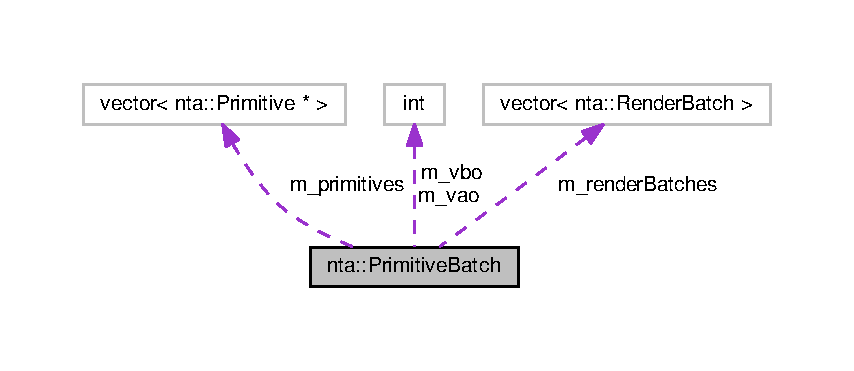
\includegraphics[width=350pt]{de/d68/classnta_1_1PrimitiveBatch__coll__graph}
\end{center}
\end{figure}


The documentation for this class was generated from the following files\+:\begin{DoxyCompactItemize}
\item 
include/nta/Primitive\+Batch.\+h\item 
src/Primitive\+Batch.\+cpp\end{DoxyCompactItemize}

\hypertarget{classnta_1_1Random}{}\section{nta\+:\+:Random Class Reference}
\label{classnta_1_1Random}\index{nta\+::\+Random@{nta\+::\+Random}}


Used for generating random numbers.  




{\ttfamily \#include $<$Random.\+h$>$}

\subsection*{Static Public Member Functions}
\begin{DoxyCompactItemize}
\item 
\mbox{\Hypertarget{classnta_1_1Random_ac310b6b657b1bdb78795d529c48f537f}\label{classnta_1_1Random_ac310b6b657b1bdb78795d529c48f537f}} 
static void \hyperlink{classnta_1_1Random_ac310b6b657b1bdb78795d529c48f537f}{init} ()
\begin{DoxyCompactList}\small\item\em initializes random number generation \end{DoxyCompactList}\item 
\mbox{\Hypertarget{classnta_1_1Random_a5cde49f2ac5cbd8d9d9844dbe7644759}\label{classnta_1_1Random_a5cde49f2ac5cbd8d9d9844dbe7644759}} 
static bool \hyperlink{classnta_1_1Random_a5cde49f2ac5cbd8d9d9844dbe7644759}{rand\+Bool} ()
\begin{DoxyCompactList}\small\item\em randomly returns true or false \end{DoxyCompactList}\item 
\mbox{\Hypertarget{classnta_1_1Random_aee5fa8d97f0cf1ccee84c6270b42a50d}\label{classnta_1_1Random_aee5fa8d97f0cf1ccee84c6270b42a50d}} 
static long \hyperlink{classnta_1_1Random_aee5fa8d97f0cf1ccee84c6270b42a50d}{rand\+Int} (long min, long max)
\begin{DoxyCompactList}\small\item\em returns a random int in the specified range exclusive (uniform distribution) \end{DoxyCompactList}\item 
\mbox{\Hypertarget{classnta_1_1Random_aa4bbbb087b7651836f53b515ffb154ad}\label{classnta_1_1Random_aa4bbbb087b7651836f53b515ffb154ad}} 
static long {\bfseries rand\+Int} (long max)
\item 
\mbox{\Hypertarget{classnta_1_1Random_aa380bcf4be06bc5b5e4707b7ae5a7907}\label{classnta_1_1Random_aa380bcf4be06bc5b5e4707b7ae5a7907}} 
static long {\bfseries rand\+Int} ()
\item 
\mbox{\Hypertarget{classnta_1_1Random_a102ed2efec77f974731e5dcdb428174a}\label{classnta_1_1Random_a102ed2efec77f974731e5dcdb428174a}} 
static float \hyperlink{classnta_1_1Random_a102ed2efec77f974731e5dcdb428174a}{rand\+Float} (float min, float max)
\begin{DoxyCompactList}\small\item\em returns a random float in the specified range (uniform distribution) \end{DoxyCompactList}\item 
\mbox{\Hypertarget{classnta_1_1Random_a6820a1c36b820baa68f7bdb2f5f5bf88}\label{classnta_1_1Random_a6820a1c36b820baa68f7bdb2f5f5bf88}} 
static float {\bfseries rand\+Float} (float max)
\item 
\mbox{\Hypertarget{classnta_1_1Random_aae9df8240d99108188bd6cb223b384a2}\label{classnta_1_1Random_aae9df8240d99108188bd6cb223b384a2}} 
static float {\bfseries rand\+Float} ()
\item 
\mbox{\Hypertarget{classnta_1_1Random_a6e12bc86e5851f01d70debf422746e0e}\label{classnta_1_1Random_a6e12bc86e5851f01d70debf422746e0e}} 
static float \hyperlink{classnta_1_1Random_a6e12bc86e5851f01d70debf422746e0e}{rand\+Gaussian} (float mean, float sd)
\begin{DoxyCompactList}\small\item\em returns a random float using the specified distribution \end{DoxyCompactList}\item 
\mbox{\Hypertarget{classnta_1_1Random_a45b43eef244823ccb5d016f79bad4ced}\label{classnta_1_1Random_a45b43eef244823ccb5d016f79bad4ced}} 
static glm\+::vec3 \hyperlink{classnta_1_1Random_a45b43eef244823ccb5d016f79bad4ced}{rand\+R\+GB} ()
\begin{DoxyCompactList}\small\item\em returns a random color \end{DoxyCompactList}\item 
\mbox{\Hypertarget{classnta_1_1Random_a6592035f3647ba9192469ea7a149c2e2}\label{classnta_1_1Random_a6592035f3647ba9192469ea7a149c2e2}} 
static glm\+::vec4 {\bfseries rand\+R\+G\+BA} ()
\item 
\mbox{\Hypertarget{classnta_1_1Random_ac4fdaa10f7d4646d4489933b48aca148}\label{classnta_1_1Random_ac4fdaa10f7d4646d4489933b48aca148}} 
static glm\+::vec2 \hyperlink{classnta_1_1Random_ac4fdaa10f7d4646d4489933b48aca148}{rand\+Vec2} (float min, float max)
\begin{DoxyCompactList}\small\item\em returna a random vector \end{DoxyCompactList}\item 
\mbox{\Hypertarget{classnta_1_1Random_a70719bc927413d2df83593c243499c88}\label{classnta_1_1Random_a70719bc927413d2df83593c243499c88}} 
static std\+::default\+\_\+random\+\_\+engine \hyperlink{classnta_1_1Random_a70719bc927413d2df83593c243499c88}{get\+R\+NG} ()
\begin{DoxyCompactList}\small\item\em returns the random number generator \end{DoxyCompactList}\end{DoxyCompactItemize}
\subsection*{Static Private Attributes}
\begin{DoxyCompactItemize}
\item 
\mbox{\Hypertarget{classnta_1_1Random_ae9a96e05f269c06af6c8dda212dae11a}\label{classnta_1_1Random_ae9a96e05f269c06af6c8dda212dae11a}} 
static std\+::default\+\_\+random\+\_\+engine {\bfseries m\+\_\+generator}
\end{DoxyCompactItemize}


\subsection{Detailed Description}
Used for generating random numbers. 

Definition at line 14 of file Random.\+h.



Collaboration diagram for nta\+:\+:Random\+:
\nopagebreak
\begin{figure}[H]
\begin{center}
\leavevmode
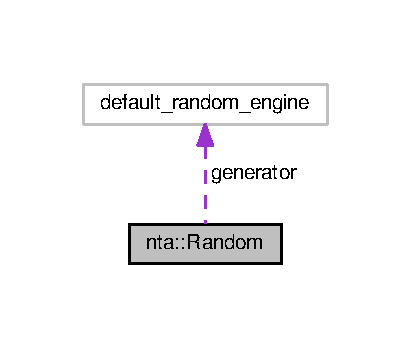
\includegraphics[width=197pt]{de/dda/classnta_1_1Random__coll__graph}
\end{center}
\end{figure}


The documentation for this class was generated from the following files\+:\begin{DoxyCompactItemize}
\item 
include/nta/Random.\+h\item 
src/Random.\+cpp\end{DoxyCompactItemize}

\hypertarget{structnta_1_1RenderBatch}{}\section{nta\+:\+:Render\+Batch Struct Reference}
\label{structnta_1_1RenderBatch}\index{nta\+::\+Render\+Batch@{nta\+::\+Render\+Batch}}


stores information about batches of vertices with the same texture in a vertex buffer object  




{\ttfamily \#include $<$Sprite\+Batch.\+h$>$}

\subsection*{Public Member Functions}
\begin{DoxyCompactItemize}
\item 
\mbox{\Hypertarget{structnta_1_1RenderBatch_a02a531d942296d7194ca96f7ed614f14}\label{structnta_1_1RenderBatch_a02a531d942296d7194ca96f7ed614f14}} 
\hyperlink{structnta_1_1RenderBatch_a02a531d942296d7194ca96f7ed614f14}{Render\+Batch} (G\+Luint t, G\+Luint o, G\+Luint n, G\+Lenum m=G\+L\+\_\+\+T\+R\+I\+A\+N\+G\+L\+ES)
\begin{DoxyCompactList}\small\item\em constructor \end{DoxyCompactList}\end{DoxyCompactItemize}
\subsection*{Public Attributes}
\begin{DoxyCompactItemize}
\item 
\mbox{\Hypertarget{structnta_1_1RenderBatch_a65aa121e11783396f753c8f937fe9d04}\label{structnta_1_1RenderBatch_a65aa121e11783396f753c8f937fe9d04}} 
G\+Luint \hyperlink{structnta_1_1RenderBatch_a65aa121e11783396f753c8f937fe9d04}{texture\+ID}
\begin{DoxyCompactList}\small\item\em the texture used by the batch \end{DoxyCompactList}\item 
\mbox{\Hypertarget{structnta_1_1RenderBatch_ab73ef79a5cbf8b60ad9991eb0a1ea9e6}\label{structnta_1_1RenderBatch_ab73ef79a5cbf8b60ad9991eb0a1ea9e6}} 
G\+Luint \hyperlink{structnta_1_1RenderBatch_ab73ef79a5cbf8b60ad9991eb0a1ea9e6}{offset}
\begin{DoxyCompactList}\small\item\em the starting point of the batch in the vertex buffer \end{DoxyCompactList}\item 
\mbox{\Hypertarget{structnta_1_1RenderBatch_a18e1cb5ff84364540a871db321557b7c}\label{structnta_1_1RenderBatch_a18e1cb5ff84364540a871db321557b7c}} 
G\+Luint \hyperlink{structnta_1_1RenderBatch_a18e1cb5ff84364540a871db321557b7c}{num\+Vertices}
\begin{DoxyCompactList}\small\item\em the number of vertices comprising the vertex buffer \end{DoxyCompactList}\item 
\mbox{\Hypertarget{structnta_1_1RenderBatch_ae2cc5e3b2e34aff278ba863443b0fdae}\label{structnta_1_1RenderBatch_ae2cc5e3b2e34aff278ba863443b0fdae}} 
G\+Lenum \hyperlink{structnta_1_1RenderBatch_ae2cc5e3b2e34aff278ba863443b0fdae}{mode}
\begin{DoxyCompactList}\small\item\em the primitive type to be drawn (G\+L\+\_\+\+P\+O\+I\+N\+TS, G\+L\+\_\+\+L\+I\+N\+ES, etc.) \end{DoxyCompactList}\end{DoxyCompactItemize}


\subsection{Detailed Description}
stores information about batches of vertices with the same texture in a vertex buffer object 

Definition at line 44 of file Sprite\+Batch.\+h.



The documentation for this struct was generated from the following file\+:\begin{DoxyCompactItemize}
\item 
include/nta/Sprite\+Batch.\+h\end{DoxyCompactItemize}

\hypertarget{classnta_1_1ResourceManager}{}\section{nta\+:\+:Resource\+Manager Class Reference}
\label{classnta_1_1ResourceManager}\index{nta\+::\+Resource\+Manager@{nta\+::\+Resource\+Manager}}


Handles storing and retrieving textures so an image isn\textquotesingle{}t loaded multiple times.  




{\ttfamily \#include $<$Resource\+Manager.\+h$>$}

\subsection*{Static Public Member Functions}
\begin{DoxyCompactItemize}
\item 
static \hyperlink{classnta_1_1Result}{Result}$<$ \hyperlink{structnta_1_1GLTexture}{G\+L\+Texture} $>$ \hyperlink{classnta_1_1ResourceManager_a60911bfeef0df3802c6ef03cc10fb5c1}{get\+Texture} (crstring image\+Path, G\+Lint min\+Filt=G\+L\+\_\+\+L\+I\+N\+E\+A\+R\+\_\+\+M\+I\+P\+M\+A\+P\+\_\+\+L\+I\+N\+E\+AR, G\+Lint mag\+Filt=G\+L\+\_\+\+L\+I\+N\+E\+AR, crvec2 dimensions=glm\+::vec2(0))
\item 
\mbox{\Hypertarget{classnta_1_1ResourceManager_ae14b4380aae490abd97d0bb1073d3a0b}\label{classnta_1_1ResourceManager_ae14b4380aae490abd97d0bb1073d3a0b}} 
static \hyperlink{classnta_1_1Result}{Result}$<$ \hyperlink{structnta_1_1GLTexture}{G\+L\+Texture} $>$ {\bfseries get\+Texture} (crstring image\+Path, crvec2 dimensions, G\+Lint min\+Filt=G\+L\+\_\+\+L\+I\+N\+E\+A\+R\+\_\+\+M\+I\+P\+M\+A\+P\+\_\+\+L\+I\+N\+E\+AR, G\+Lint mag\+Filt=G\+L\+\_\+\+L\+I\+N\+E\+AR)
\item 
\mbox{\Hypertarget{classnta_1_1ResourceManager_a5a9625aa03f75fad3d34c0ce222014e9}\label{classnta_1_1ResourceManager_a5a9625aa03f75fad3d34c0ce222014e9}} 
static \hyperlink{classnta_1_1Result}{Result}$<$ std\+::string $>$ {\bfseries get\+File} (\hyperlink{structnta_1_1GLTexture}{G\+L\+Texture} tex)
\item 
\mbox{\Hypertarget{classnta_1_1ResourceManager_a0411e5cf357d6d285820338d92d06a0e}\label{classnta_1_1ResourceManager_a0411e5cf357d6d285820338d92d06a0e}} 
static \hyperlink{classnta_1_1SpriteFont}{Sprite\+Font} $\ast$ {\bfseries get\+Sprite\+Font} (crstring font\+Path, int font\+Size=32)
\item 
\mbox{\Hypertarget{classnta_1_1ResourceManager_a2f9971f86fc9e50d7a62aa5f6f91a489}\label{classnta_1_1ResourceManager_a2f9971f86fc9e50d7a62aa5f6f91a489}} 
static void \hyperlink{classnta_1_1ResourceManager_a2f9971f86fc9e50d7a62aa5f6f91a489}{delete\+Texture} (crstring image\+Path)
\begin{DoxyCompactList}\small\item\em removes the resource with the given path from the map and deletes it \end{DoxyCompactList}\item 
\mbox{\Hypertarget{classnta_1_1ResourceManager_a16c549cb1496d1f38b5900258b0624c7}\label{classnta_1_1ResourceManager_a16c549cb1496d1f38b5900258b0624c7}} 
static void {\bfseries delete\+Sprite\+Font} (crstring font\+Path, int font\+Size=32)
\item 
\mbox{\Hypertarget{classnta_1_1ResourceManager_a26ff6f1cb4044d8f47fa5db9a3df2514}\label{classnta_1_1ResourceManager_a26ff6f1cb4044d8f47fa5db9a3df2514}} 
static void {\bfseries destroy} ()
\end{DoxyCompactItemize}
\subsection*{Static Private Attributes}
\begin{DoxyCompactItemize}
\item 
\mbox{\Hypertarget{classnta_1_1ResourceManager_abf9bb10402834f05b2673e0c1d8cb9aa}\label{classnta_1_1ResourceManager_abf9bb10402834f05b2673e0c1d8cb9aa}} 
static std\+::map$<$ std\+::string, \hyperlink{structnta_1_1GLTexture}{G\+L\+Texture} $>$ \hyperlink{classnta_1_1ResourceManager_abf9bb10402834f05b2673e0c1d8cb9aa}{m\+\_\+texture\+Map}
\begin{DoxyCompactList}\small\item\em a map for associating a texture with the name of its file \end{DoxyCompactList}\item 
\mbox{\Hypertarget{classnta_1_1ResourceManager_a4255640b4c0ba44f1ad8289d3d912897}\label{classnta_1_1ResourceManager_a4255640b4c0ba44f1ad8289d3d912897}} 
static std\+::unordered\+\_\+map$<$ \hyperlink{structnta_1_1GLTexture}{G\+L\+Texture}, std\+::string $>$ \hyperlink{classnta_1_1ResourceManager_a4255640b4c0ba44f1ad8289d3d912897}{m\+\_\+texture\+Files}
\begin{DoxyCompactList}\small\item\em Inverse map to m\+\_\+texture\+Map. \end{DoxyCompactList}\item 
\mbox{\Hypertarget{classnta_1_1ResourceManager_ac6a87b69211ba52452b4c02847ea934e}\label{classnta_1_1ResourceManager_ac6a87b69211ba52452b4c02847ea934e}} 
static std\+::map$<$ std\+::pair$<$ std\+::string, int $>$, \hyperlink{classnta_1_1SpriteFont}{Sprite\+Font} $\ast$ $>$ \hyperlink{classnta_1_1ResourceManager_ac6a87b69211ba52452b4c02847ea934e}{m\+\_\+font\+Map}
\begin{DoxyCompactList}\small\item\em Why does this hold pointers? \end{DoxyCompactList}\end{DoxyCompactItemize}


\subsection{Detailed Description}
Handles storing and retrieving textures so an image isn\textquotesingle{}t loaded multiple times. 

Definition at line 12 of file Resource\+Manager.\+h.



Collaboration diagram for nta\+:\+:Resource\+Manager\+:
\nopagebreak
\begin{figure}[H]
\begin{center}
\leavevmode
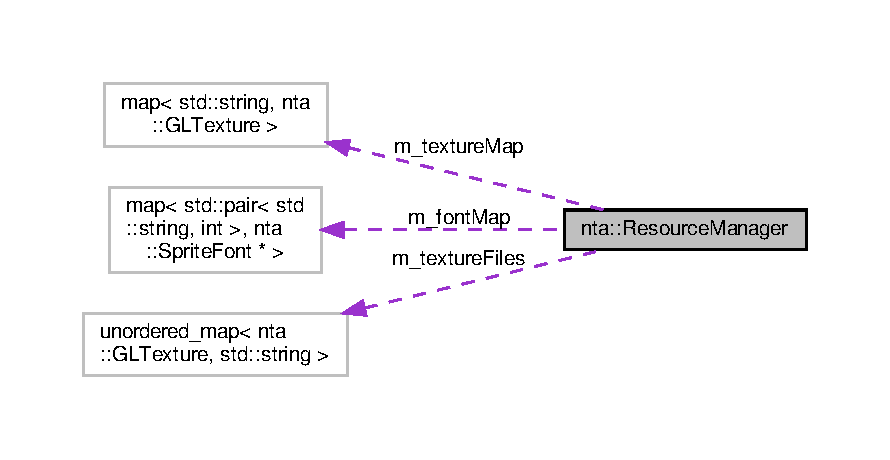
\includegraphics[width=350pt]{d2/d39/classnta_1_1ResourceManager__coll__graph}
\end{center}
\end{figure}


\subsection{Member Function Documentation}
\mbox{\Hypertarget{classnta_1_1ResourceManager_a60911bfeef0df3802c6ef03cc10fb5c1}\label{classnta_1_1ResourceManager_a60911bfeef0df3802c6ef03cc10fb5c1}} 
\index{nta\+::\+Resource\+Manager@{nta\+::\+Resource\+Manager}!get\+Texture@{get\+Texture}}
\index{get\+Texture@{get\+Texture}!nta\+::\+Resource\+Manager@{nta\+::\+Resource\+Manager}}
\subsubsection{\texorpdfstring{get\+Texture()}{getTexture()}}
{\footnotesize\ttfamily \hyperlink{classnta_1_1Result}{Result}$<$ \hyperlink{structnta_1_1GLTexture}{G\+L\+Texture} $>$ nta\+::\+Resource\+Manager\+::get\+Texture (\begin{DoxyParamCaption}\item[{crstring}]{image\+Path,  }\item[{G\+Lint}]{min\+Filt = {\ttfamily GL\+\_\+LINEAR\+\_\+MIPMAP\+\_\+LINEAR},  }\item[{G\+Lint}]{mag\+Filt = {\ttfamily GL\+\_\+LINEAR},  }\item[{crvec2}]{dimensions = {\ttfamily glm\+:\+:vec2(0)} }\end{DoxyParamCaption})\hspace{0.3cm}{\ttfamily [static]}}

returns the resource with the given path, loading it if need be  Why was I returning references before? 

Definition at line 8 of file Resource\+Manager.\+cpp.



Referenced by nta\+::\+Sprite\+::init().

Here is the call graph for this function\+:
\nopagebreak
\begin{figure}[H]
\begin{center}
\leavevmode
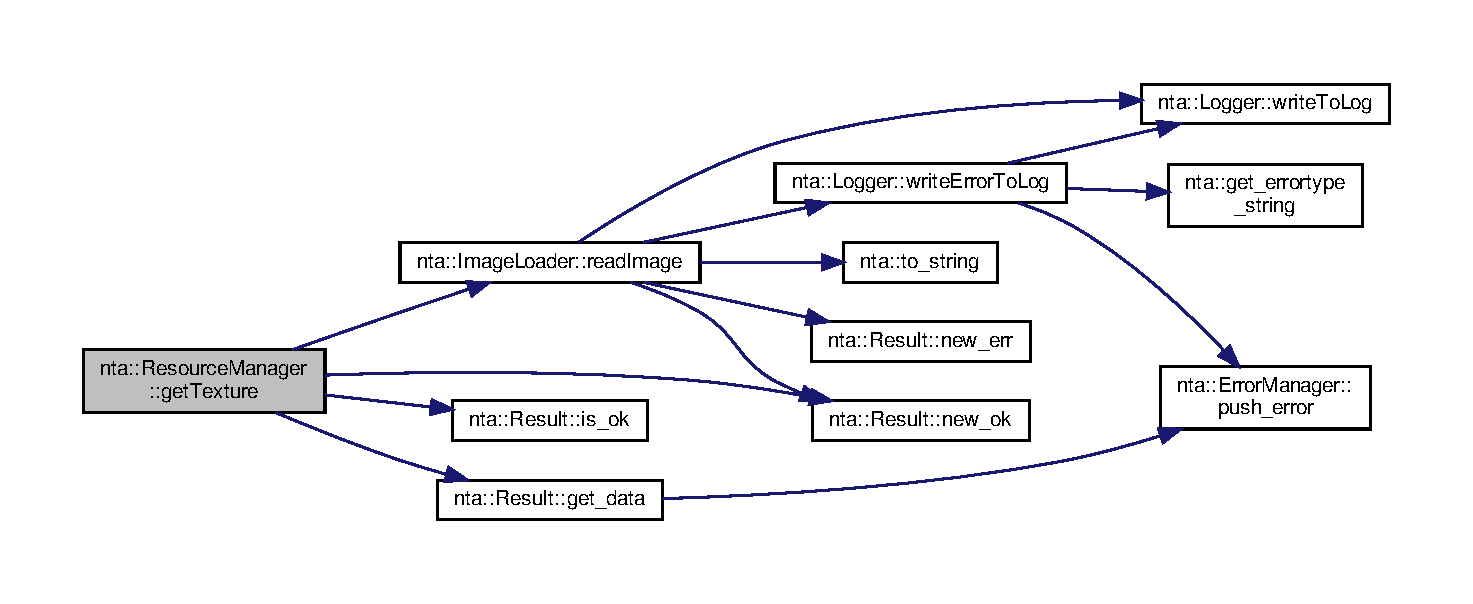
\includegraphics[width=350pt]{d5/d87/classnta_1_1ResourceManager_a60911bfeef0df3802c6ef03cc10fb5c1_cgraph}
\end{center}
\end{figure}
Here is the caller graph for this function\+:\nopagebreak
\begin{figure}[H]
\begin{center}
\leavevmode
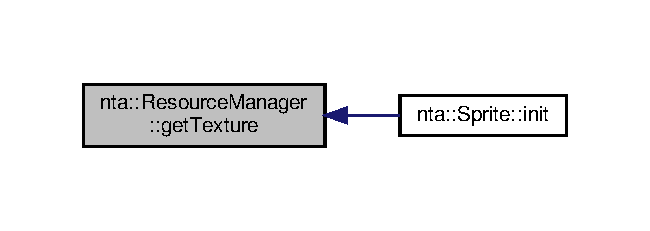
\includegraphics[width=312pt]{d5/d87/classnta_1_1ResourceManager_a60911bfeef0df3802c6ef03cc10fb5c1_icgraph}
\end{center}
\end{figure}


The documentation for this class was generated from the following files\+:\begin{DoxyCompactItemize}
\item 
include/nta/Resource\+Manager.\+h\item 
src/Resource\+Manager.\+cpp\end{DoxyCompactItemize}

\hypertarget{classnta_1_1Result}{}\section{nta\+:\+:Result$<$ T $>$ Class Template Reference}
\label{classnta_1_1Result}\index{nta\+::\+Result$<$ T $>$@{nta\+::\+Result$<$ T $>$}}


{\ttfamily \#include $<$Errors.\+h$>$}

\subsection*{Public Member Functions}
\begin{DoxyCompactItemize}
\item 
\mbox{\Hypertarget{classnta_1_1Result_a2410d4b139bc036b9ff6d30ab5e15f8d}\label{classnta_1_1Result_a2410d4b139bc036b9ff6d30ab5e15f8d}} 
\hyperlink{classnta_1_1Result_a2410d4b139bc036b9ff6d30ab5e15f8d}{Result} (const \hyperlink{classnta_1_1Result}{Result} \&other)
\begin{DoxyCompactList}\small\item\em Public copy constructor. \end{DoxyCompactList}\item 
\mbox{\Hypertarget{classnta_1_1Result_a5fd9525155666ef2eaf605d82d13bd77}\label{classnta_1_1Result_a5fd9525155666ef2eaf605d82d13bd77}} 
\hyperlink{classnta_1_1Result_a5fd9525155666ef2eaf605d82d13bd77}{$\sim$\+Result} ()
\begin{DoxyCompactList}\small\item\em Public destructor. \end{DoxyCompactList}\item 
\mbox{\Hypertarget{classnta_1_1Result_ab742b047f1e670bc6a374f32c3fd48ea}\label{classnta_1_1Result_ab742b047f1e670bc6a374f32c3fd48ea}} 
bool \hyperlink{classnta_1_1Result_ab742b047f1e670bc6a374f32c3fd48ea}{is\+\_\+err} () const
\begin{DoxyCompactList}\small\item\em Is this an \hyperlink{structnta_1_1Error}{Error}. \end{DoxyCompactList}\item 
\mbox{\Hypertarget{classnta_1_1Result_a61deaa087694eae4fdaece2996fedda0}\label{classnta_1_1Result_a61deaa087694eae4fdaece2996fedda0}} 
bool \hyperlink{classnta_1_1Result_a61deaa087694eae4fdaece2996fedda0}{is\+\_\+ok} () const
\begin{DoxyCompactList}\small\item\em Is this normal data. \end{DoxyCompactList}\item 
\mbox{\Hypertarget{classnta_1_1Result_a96baacea35085048d694279d5de8c82e}\label{classnta_1_1Result_a96baacea35085048d694279d5de8c82e}} 
T \hyperlink{classnta_1_1Result_a96baacea35085048d694279d5de8c82e}{get\+\_\+data} () const
\begin{DoxyCompactList}\small\item\em Get the data (only use if \hyperlink{classnta_1_1Result_a61deaa087694eae4fdaece2996fedda0}{is\+\_\+ok()} returns true) \end{DoxyCompactList}\item 
\mbox{\Hypertarget{classnta_1_1Result_a9ea9717e77d5e9a2371eb3cf9c896bc7}\label{classnta_1_1Result_a9ea9717e77d5e9a2371eb3cf9c896bc7}} 
\hyperlink{structnta_1_1Error}{Error} \hyperlink{classnta_1_1Result_a9ea9717e77d5e9a2371eb3cf9c896bc7}{get\+\_\+err} () const
\begin{DoxyCompactList}\small\item\em Get the \hyperlink{structnta_1_1Error}{Error} (only use if \hyperlink{classnta_1_1Result_ab742b047f1e670bc6a374f32c3fd48ea}{is\+\_\+err()} returns true) \end{DoxyCompactList}\item 
\mbox{\Hypertarget{classnta_1_1Result_ae5fb7648fc0ecfbab99404a97fb27c83}\label{classnta_1_1Result_ae5fb7648fc0ecfbab99404a97fb27c83}} 
T \hyperlink{classnta_1_1Result_ae5fb7648fc0ecfbab99404a97fb27c83}{get\+\_\+data\+\_\+or} (T optb) const
\begin{DoxyCompactList}\small\item\em Tries getting data, returning a default value if this is an error. \end{DoxyCompactList}\end{DoxyCompactItemize}
\subsection*{Static Public Member Functions}
\begin{DoxyCompactItemize}
\item 
static \hyperlink{classnta_1_1Result}{Result} \hyperlink{classnta_1_1Result_af193a336ab789de94a975c6f0a039e40}{new\+\_\+ok} (const T \&data)
\item 
static \hyperlink{classnta_1_1Result}{Result} \hyperlink{classnta_1_1Result_ad65a9140ae2a03cfb13bd30f848b1aa5}{new\+\_\+err} (const \hyperlink{structnta_1_1Error}{Error} \&err)
\end{DoxyCompactItemize}
\subsection*{Private Member Functions}
\begin{DoxyCompactItemize}
\item 
\mbox{\Hypertarget{classnta_1_1Result_a6bb10dacafbf334b7209adc5615de44e}\label{classnta_1_1Result_a6bb10dacafbf334b7209adc5615de44e}} 
\hyperlink{classnta_1_1Result_a6bb10dacafbf334b7209adc5615de44e}{Result} ()
\begin{DoxyCompactList}\small\item\em Private constructor (use new\+\_\+ok or new\+\_\+err) \end{DoxyCompactList}\end{DoxyCompactItemize}
\subsection*{Private Attributes}
\begin{DoxyCompactItemize}
\item 
\mbox{\Hypertarget{classnta_1_1Result_a225adf68d093d584826f4aab98cacf97}\label{classnta_1_1Result_a225adf68d093d584826f4aab98cacf97}} 
\begin{tabbing}
xx\=xx\=xx\=xx\=xx\=xx\=xx\=xx\=xx\=\kill
union \{\\
\mbox{\Hypertarget{classnta_1_1Result_ab084104dfedebe7715d97987595ad147}\label{classnta_1_1Result_ab084104dfedebe7715d97987595ad147}} 
T {\bfseries data}\\
\mbox{\Hypertarget{classnta_1_1Result_acd60a522df7b4adf81729de1dc626955}\label{classnta_1_1Result_acd60a522df7b4adf81729de1dc626955}} 
\hyperlink{structnta_1_1Error}{Error} {\bfseries err}\\
\}; \\

\end{tabbing}\begin{DoxyCompactList}\small\item\em The data or error held by this \hyperlink{classnta_1_1Result}{Result}. \end{DoxyCompactList}\item 
\mbox{\Hypertarget{classnta_1_1Result_a27f85dc35976426c1f5c01431ac2e1cc}\label{classnta_1_1Result_a27f85dc35976426c1f5c01431ac2e1cc}} 
bool \hyperlink{classnta_1_1Result_a27f85dc35976426c1f5c01431ac2e1cc}{is\+\_\+err\+\_\+variant}
\begin{DoxyCompactList}\small\item\em Whether or not an error occured. \end{DoxyCompactList}\end{DoxyCompactItemize}


\subsection{Detailed Description}
\subsubsection*{template$<$typename T$>$\newline
class nta\+::\+Result$<$ T $>$}

Used for returning data when an error could potentially occur \begin{DoxyRefDesc}{Todo}
\item[\hyperlink{todo__todo000005}{Todo}]Use \hyperlink{classnta_1_1Result}{Result} type everywhere it needs to be used \end{DoxyRefDesc}


Definition at line 74 of file Errors.\+h.



Collaboration diagram for nta\+:\+:Result$<$ T $>$\+:\nopagebreak
\begin{figure}[H]
\begin{center}
\leavevmode
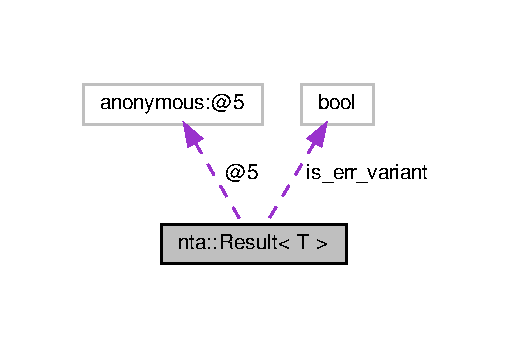
\includegraphics[width=246pt]{d6/da5/classnta_1_1Result__coll__graph}
\end{center}
\end{figure}


\subsection{Member Function Documentation}
\mbox{\Hypertarget{classnta_1_1Result_ad65a9140ae2a03cfb13bd30f848b1aa5}\label{classnta_1_1Result_ad65a9140ae2a03cfb13bd30f848b1aa5}} 
\index{nta\+::\+Result@{nta\+::\+Result}!new\+\_\+err@{new\+\_\+err}}
\index{new\+\_\+err@{new\+\_\+err}!nta\+::\+Result@{nta\+::\+Result}}
\subsubsection{\texorpdfstring{new\+\_\+err()}{new\_err()}}
{\footnotesize\ttfamily template$<$typename T$>$ \\
static \hyperlink{classnta_1_1Result}{Result} \hyperlink{classnta_1_1Result}{nta\+::\+Result}$<$ T $>$\+::new\+\_\+err (\begin{DoxyParamCaption}\item[{const \hyperlink{structnta_1_1Error}{Error} \&}]{err }\end{DoxyParamCaption})\hspace{0.3cm}{\ttfamily [inline]}, {\ttfamily [static]}}

Create new \hyperlink{classnta_1_1Result}{Result} holding an \hyperlink{structnta_1_1Error}{Error} This takes ownership of the err passed in 

Definition at line 109 of file Errors.\+h.



Referenced by nta\+::\+Resource\+Manager\+::get\+Texture(), and nta\+::\+Image\+Loader\+::read\+Image().

Here is the caller graph for this function\+:\nopagebreak
\begin{figure}[H]
\begin{center}
\leavevmode
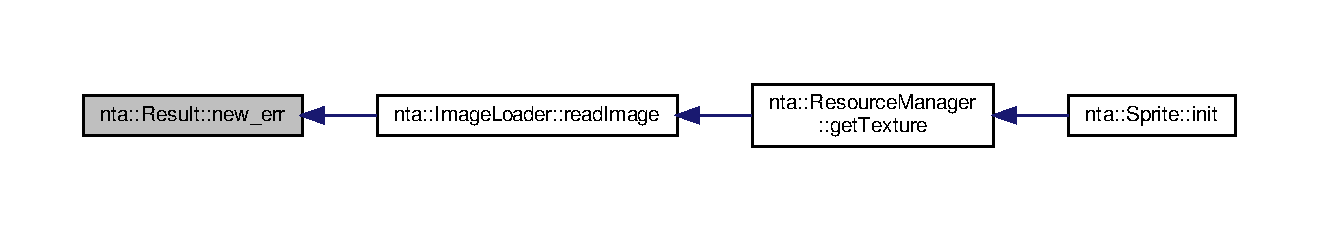
\includegraphics[width=350pt]{d8/d2e/classnta_1_1Result_ad65a9140ae2a03cfb13bd30f848b1aa5_icgraph}
\end{center}
\end{figure}
\mbox{\Hypertarget{classnta_1_1Result_af193a336ab789de94a975c6f0a039e40}\label{classnta_1_1Result_af193a336ab789de94a975c6f0a039e40}} 
\index{nta\+::\+Result@{nta\+::\+Result}!new\+\_\+ok@{new\+\_\+ok}}
\index{new\+\_\+ok@{new\+\_\+ok}!nta\+::\+Result@{nta\+::\+Result}}
\subsubsection{\texorpdfstring{new\+\_\+ok()}{new\_ok()}}
{\footnotesize\ttfamily template$<$typename T$>$ \\
static \hyperlink{classnta_1_1Result}{Result} \hyperlink{classnta_1_1Result}{nta\+::\+Result}$<$ T $>$\+::new\+\_\+ok (\begin{DoxyParamCaption}\item[{const T \&}]{data }\end{DoxyParamCaption})\hspace{0.3cm}{\ttfamily [inline]}, {\ttfamily [static]}}

Create new \hyperlink{classnta_1_1Result}{Result} holding normal data This takes ownership of the data passed in 

Definition at line 100 of file Errors.\+h.



Referenced by nta\+::\+Resource\+Manager\+::get\+Texture(), and nta\+::\+Image\+Loader\+::read\+Image().

Here is the caller graph for this function\+:\nopagebreak
\begin{figure}[H]
\begin{center}
\leavevmode
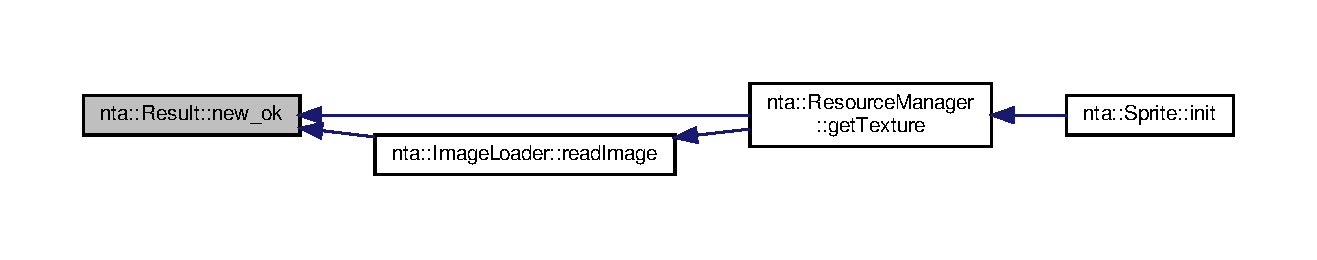
\includegraphics[width=350pt]{d8/d2e/classnta_1_1Result_af193a336ab789de94a975c6f0a039e40_icgraph}
\end{center}
\end{figure}


The documentation for this class was generated from the following file\+:\begin{DoxyCompactItemize}
\item 
include/nta/Errors.\+h\end{DoxyCompactItemize}

\hypertarget{classnta_1_1Screen}{}\section{nta\+:\+:Screen Class Reference}
\label{classnta_1_1Screen}\index{nta\+::\+Screen@{nta\+::\+Screen}}


Represents a game screen.  




{\ttfamily \#include $<$Screen.\+h$>$}

\subsection*{Public Member Functions}
\begin{DoxyCompactItemize}
\item 
\mbox{\Hypertarget{classnta_1_1Screen_a86944d19cec1189fee2945a4f8dae477}\label{classnta_1_1Screen_a86944d19cec1189fee2945a4f8dae477}} 
\hyperlink{classnta_1_1Screen_a86944d19cec1189fee2945a4f8dae477}{Screen} ()
\begin{DoxyCompactList}\small\item\em basic constructor and destructor \end{DoxyCompactList}\item 
\mbox{\Hypertarget{classnta_1_1Screen_a2d53fc8f7ac43307896863fd6b3cad1c}\label{classnta_1_1Screen_a2d53fc8f7ac43307896863fd6b3cad1c}} 
Screen\+State \hyperlink{classnta_1_1Screen_a2d53fc8f7ac43307896863fd6b3cad1c}{get\+State} () const
\begin{DoxyCompactList}\small\item\em returns state of screen \end{DoxyCompactList}\item 
\mbox{\Hypertarget{classnta_1_1Screen_a506f2266b008ccd071f630a5c252567e}\label{classnta_1_1Screen_a506f2266b008ccd071f630a5c252567e}} 
int \hyperlink{classnta_1_1Screen_a506f2266b008ccd071f630a5c252567e}{get\+Esc\+Index} () const
\begin{DoxyCompactList}\small\item\em sets/gets various screen indices \end{DoxyCompactList}\item 
\mbox{\Hypertarget{classnta_1_1Screen_a01f4fdd4cadd6abe4fef2605a0fde52a}\label{classnta_1_1Screen_a01f4fdd4cadd6abe4fef2605a0fde52a}} 
int {\bfseries get\+X\+Index} () const
\item 
\mbox{\Hypertarget{classnta_1_1Screen_aba9c09cd06dfc05557b86d866a7fb2b9}\label{classnta_1_1Screen_aba9c09cd06dfc05557b86d866a7fb2b9}} 
int {\bfseries get\+Next\+Index} () const
\item 
\mbox{\Hypertarget{classnta_1_1Screen_ae149bdd787f8f41b45c667faef971326}\label{classnta_1_1Screen_ae149bdd787f8f41b45c667faef971326}} 
int {\bfseries get\+Index} () const
\item 
\mbox{\Hypertarget{classnta_1_1Screen_a9c9329a6700fbed8ab6513d471835bfa}\label{classnta_1_1Screen_a9c9329a6700fbed8ab6513d471835bfa}} 
void \hyperlink{classnta_1_1Screen_a9c9329a6700fbed8ab6513d471835bfa}{set\+Manager} (\hyperlink{classnta_1_1ScreenManager}{Screen\+Manager} $\ast$manager, \hyperlink{classnta_1_1SetManagerKey}{Set\+Manager\+Key} key)
\begin{DoxyCompactList}\small\item\em Sets the manager of this screen. \end{DoxyCompactList}\item 
\mbox{\Hypertarget{classnta_1_1Screen_a06a0cb178a3bedde883e7a9b5c825a3d}\label{classnta_1_1Screen_a06a0cb178a3bedde883e7a9b5c825a3d}} 
void {\bfseries set\+Indices} (int index, int esc\+Index, int x\+Index)
\item 
\mbox{\Hypertarget{classnta_1_1Screen_a3c74cd84437e8897850ce4bae98bc8b2}\label{classnta_1_1Screen_a3c74cd84437e8897850ce4bae98bc8b2}} 
void \hyperlink{classnta_1_1Screen_a3c74cd84437e8897850ce4bae98bc8b2}{set\+Window} (crstring title)
\begin{DoxyCompactList}\small\item\em sets the window to associate with this screen \end{DoxyCompactList}\item 
\mbox{\Hypertarget{classnta_1_1Screen_a323ff61ac31f55bd39fa818ccd8200fb}\label{classnta_1_1Screen_a323ff61ac31f55bd39fa818ccd8200fb}} 
virtual void \hyperlink{classnta_1_1Screen_a323ff61ac31f55bd39fa818ccd8200fb}{render} ()=0
\begin{DoxyCompactList}\small\item\em renders screen \end{DoxyCompactList}\item 
\mbox{\Hypertarget{classnta_1_1Screen_a6892f9b74b033d8bd5f4e9f190d49efa}\label{classnta_1_1Screen_a6892f9b74b033d8bd5f4e9f190d49efa}} 
virtual void \hyperlink{classnta_1_1Screen_a6892f9b74b033d8bd5f4e9f190d49efa}{update} ()=0
\begin{DoxyCompactList}\small\item\em updates screen \end{DoxyCompactList}\item 
\mbox{\Hypertarget{classnta_1_1Screen_a645ccabe314f6c9084b493617c3eeafe}\label{classnta_1_1Screen_a645ccabe314f6c9084b493617c3eeafe}} 
virtual void \hyperlink{classnta_1_1Screen_a645ccabe314f6c9084b493617c3eeafe}{handle\+Input} ()
\begin{DoxyCompactList}\small\item\em handles user input \end{DoxyCompactList}\item 
\mbox{\Hypertarget{classnta_1_1Screen_af29956d6f8ac437ef2f26c9d0973e509}\label{classnta_1_1Screen_af29956d6f8ac437ef2f26c9d0973e509}} 
virtual void \hyperlink{classnta_1_1Screen_af29956d6f8ac437ef2f26c9d0973e509}{on\+Focus} ()
\begin{DoxyCompactList}\small\item\em called when the screen becomes active \end{DoxyCompactList}\item 
\mbox{\Hypertarget{classnta_1_1Screen_a172d24c2224aef718d151b621379def1}\label{classnta_1_1Screen_a172d24c2224aef718d151b621379def1}} 
virtual void \hyperlink{classnta_1_1Screen_a172d24c2224aef718d151b621379def1}{off\+Focus} ()
\begin{DoxyCompactList}\small\item\em called when the screen is no longer active \end{DoxyCompactList}\item 
\mbox{\Hypertarget{classnta_1_1Screen_ae749bdd554cea6beb81ed8bcd1cd4ed1}\label{classnta_1_1Screen_ae749bdd554cea6beb81ed8bcd1cd4ed1}} 
virtual void \hyperlink{classnta_1_1Screen_ae749bdd554cea6beb81ed8bcd1cd4ed1}{init} ()=0
\begin{DoxyCompactList}\small\item\em initializes the screen \end{DoxyCompactList}\end{DoxyCompactItemize}
\subsection*{Protected Attributes}
\begin{DoxyCompactItemize}
\item 
\mbox{\Hypertarget{classnta_1_1Screen_a68d2c095aadfb248263f43cb12cd34a1}\label{classnta_1_1Screen_a68d2c095aadfb248263f43cb12cd34a1}} 
Screen\+State \hyperlink{classnta_1_1Screen_a68d2c095aadfb248263f43cb12cd34a1}{m\+\_\+state} = Screen\+State\+::\+N\+O\+NE
\begin{DoxyCompactList}\small\item\em the state of this screen \end{DoxyCompactList}\item 
\mbox{\Hypertarget{classnta_1_1Screen_a712bfbeb6f85d9c4229de9b974b05e58}\label{classnta_1_1Screen_a712bfbeb6f85d9c4229de9b974b05e58}} 
\hyperlink{classnta_1_1Window}{Window} $\ast$ \hyperlink{classnta_1_1Screen_a712bfbeb6f85d9c4229de9b974b05e58}{m\+\_\+window} = nullptr
\begin{DoxyCompactList}\small\item\em the window the screen is rendered in \end{DoxyCompactList}\item 
\mbox{\Hypertarget{classnta_1_1Screen_a3496a69b02f4b120d907042d3201deff}\label{classnta_1_1Screen_a3496a69b02f4b120d907042d3201deff}} 
\hyperlink{classnta_1_1ScreenManager}{Screen\+Manager} $\ast$ \hyperlink{classnta_1_1Screen_a3496a69b02f4b120d907042d3201deff}{m\+\_\+manager} = nullptr
\begin{DoxyCompactList}\small\item\em the \hyperlink{classnta_1_1ScreenManager}{Screen\+Manager} that owns this screen \end{DoxyCompactList}\item 
\mbox{\Hypertarget{classnta_1_1Screen_a6be3b899f3bc9e531d64676cbbd6815e}\label{classnta_1_1Screen_a6be3b899f3bc9e531d64676cbbd6815e}} 
int \hyperlink{classnta_1_1Screen_a6be3b899f3bc9e531d64676cbbd6815e}{m\+\_\+next\+Index} = -\/1
\begin{DoxyCompactList}\small\item\em the index of the screen to go to in special circumstances \end{DoxyCompactList}\end{DoxyCompactItemize}
\subsection*{Private Attributes}
\begin{DoxyCompactItemize}
\item 
\mbox{\Hypertarget{classnta_1_1Screen_a60c7a5b3894ec6f42042dac0f1f3c54c}\label{classnta_1_1Screen_a60c7a5b3894ec6f42042dac0f1f3c54c}} 
int \hyperlink{classnta_1_1Screen_a60c7a5b3894ec6f42042dac0f1f3c54c}{m\+\_\+index} = -\/1
\begin{DoxyCompactList}\small\item\em the index of this screen in its container \end{DoxyCompactList}\item 
\mbox{\Hypertarget{classnta_1_1Screen_a5e38ecb4efb8ea6487774052f9d3281d}\label{classnta_1_1Screen_a5e38ecb4efb8ea6487774052f9d3281d}} 
int \hyperlink{classnta_1_1Screen_a5e38ecb4efb8ea6487774052f9d3281d}{m\+\_\+esc\+Index} = -\/1
\begin{DoxyCompactList}\small\item\em the index of the screen to go to when the Esc key is pressed \end{DoxyCompactList}\item 
\mbox{\Hypertarget{classnta_1_1Screen_afba24e281f497022a32416f707785b9c}\label{classnta_1_1Screen_afba24e281f497022a32416f707785b9c}} 
int \hyperlink{classnta_1_1Screen_afba24e281f497022a32416f707785b9c}{m\+\_\+x\+Index} = -\/1
\begin{DoxyCompactList}\small\item\em the index of the screen to go to when the window\textquotesingle{}s X button is pressed \end{DoxyCompactList}\end{DoxyCompactItemize}


\subsection{Detailed Description}
Represents a game screen. 

Definition at line 17 of file Screen.\+h.



Collaboration diagram for nta\+:\+:Screen\+:\nopagebreak
\begin{figure}[H]
\begin{center}
\leavevmode
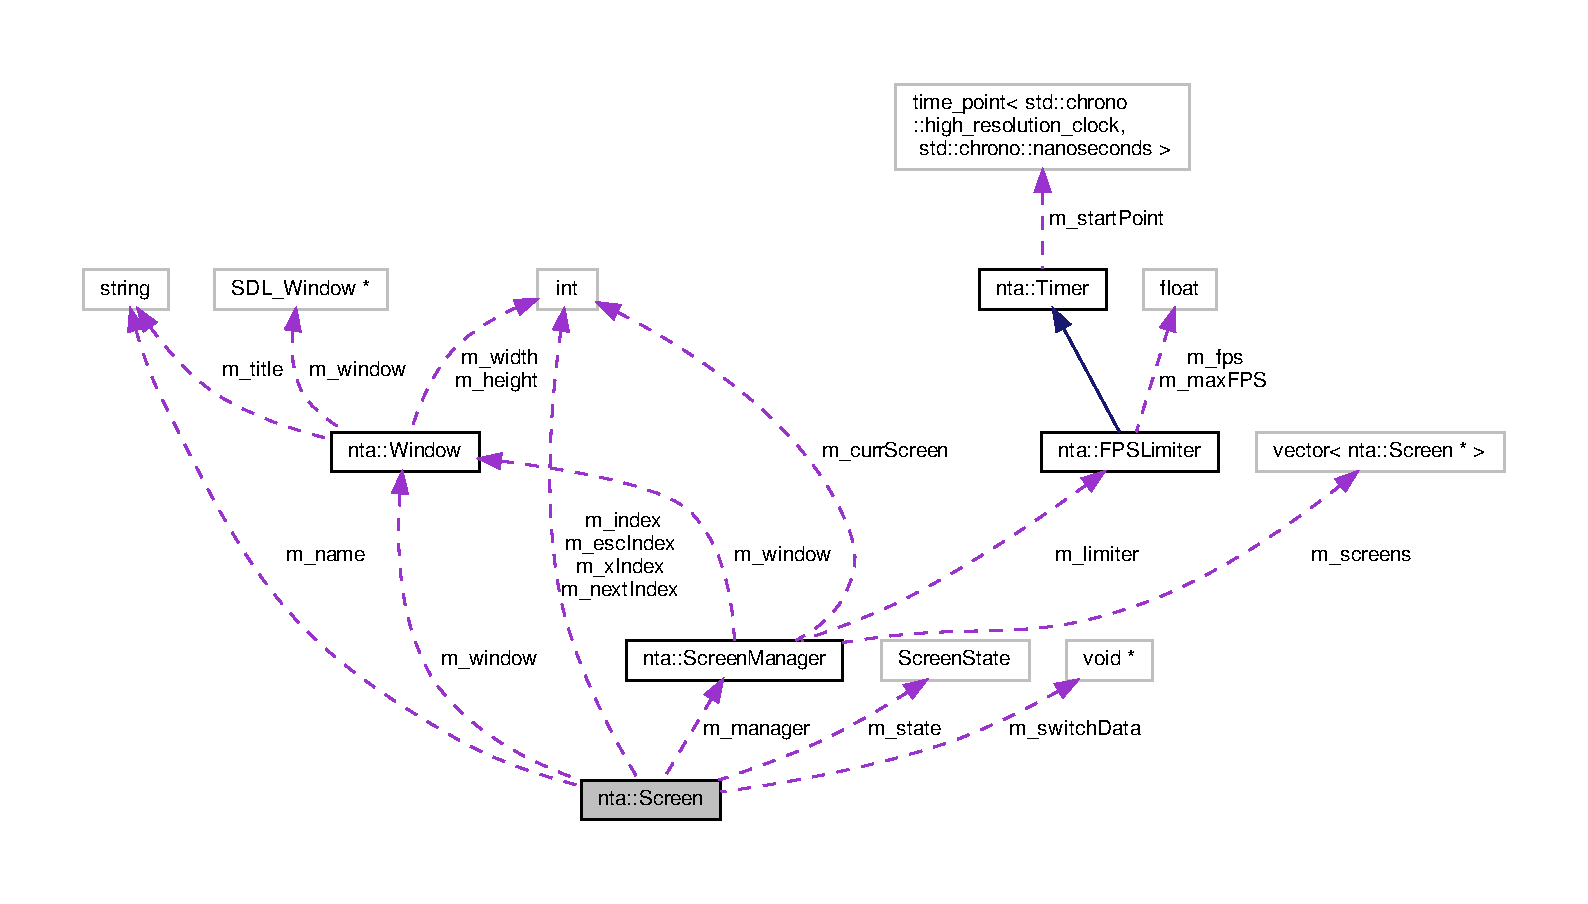
\includegraphics[width=350pt]{d4/df6/classnta_1_1Screen__coll__graph}
\end{center}
\end{figure}


The documentation for this class was generated from the following files\+:\begin{DoxyCompactItemize}
\item 
include/nta/Screen.\+h\item 
src/Screen.\+cpp\end{DoxyCompactItemize}

\hypertarget{classnta_1_1ScreenManager}{}\section{nta\+:\+:Screen\+Manager Class Reference}
\label{classnta_1_1ScreenManager}\index{nta\+::\+Screen\+Manager@{nta\+::\+Screen\+Manager}}


Manages a collection of screens.  




{\ttfamily \#include $<$Screen\+Manager.\+h$>$}

\subsection*{Public Member Functions}
\begin{DoxyCompactItemize}
\item 
\mbox{\Hypertarget{classnta_1_1ScreenManager_a46a7adb4a69fea8e074fa2251c815bad}\label{classnta_1_1ScreenManager_a46a7adb4a69fea8e074fa2251c815bad}} 
\hyperlink{classnta_1_1ScreenManager_a46a7adb4a69fea8e074fa2251c815bad}{Screen\+Manager} (crstring title, float max\+F\+PS)
\begin{DoxyCompactList}\small\item\em sets the max fps and the window to use \end{DoxyCompactList}\item 
\mbox{\Hypertarget{classnta_1_1ScreenManager_aea609a639ffdc377e798eda054e6a4ba}\label{classnta_1_1ScreenManager_aea609a639ffdc377e798eda054e6a4ba}} 
\hyperlink{classnta_1_1ScreenManager_aea609a639ffdc377e798eda054e6a4ba}{$\sim$\+Screen\+Manager} ()
\begin{DoxyCompactList}\small\item\em basic destructor \end{DoxyCompactList}\item 
\hyperlink{classnta_1_1Screen}{Screen} $\ast$ \hyperlink{classnta_1_1ScreenManager_a4b26e8adc481bfb37a088e047e4ccc2a}{get\+Curr\+Screen} () const
\begin{DoxyCompactList}\small\item\em returns the active screen \end{DoxyCompactList}\item 
\mbox{\Hypertarget{classnta_1_1ScreenManager_a24e61f523b383277b7284cab76ad9e5a}\label{classnta_1_1ScreenManager_a24e61f523b383277b7284cab76ad9e5a}} 
float \hyperlink{classnta_1_1ScreenManager_a24e61f523b383277b7284cab76ad9e5a}{get\+F\+PS} () const
\begin{DoxyCompactList}\small\item\em returns the current fps \end{DoxyCompactList}\item 
\mbox{\Hypertarget{classnta_1_1ScreenManager_a18659a2edcddd60d53094ac46ac0b0df}\label{classnta_1_1ScreenManager_a18659a2edcddd60d53094ac46ac0b0df}} 
void \hyperlink{classnta_1_1ScreenManager_a18659a2edcddd60d53094ac46ac0b0df}{add\+Screen} (\hyperlink{classnta_1_1Screen}{Screen} $\ast$new\+Screen, int esc\+Index=-\/1, int x\+Index=-\/1, crstring title=\char`\"{}\char`\"{})
\begin{DoxyCompactList}\small\item\em adds a screen and sets some of its properties \end{DoxyCompactList}\item 
\mbox{\Hypertarget{classnta_1_1ScreenManager_a97edbb147671d2b94e1f5a13cb6f7660}\label{classnta_1_1ScreenManager_a97edbb147671d2b94e1f5a13cb6f7660}} 
void \hyperlink{classnta_1_1ScreenManager_a97edbb147671d2b94e1f5a13cb6f7660}{switch\+Screen} (int new\+Index)
\begin{DoxyCompactList}\small\item\em switches the to a new screen \end{DoxyCompactList}\item 
\mbox{\Hypertarget{classnta_1_1ScreenManager_ad4e28094d9293b55f38ea463ac802219}\label{classnta_1_1ScreenManager_ad4e28094d9293b55f38ea463ac802219}} 
void \hyperlink{classnta_1_1ScreenManager_ad4e28094d9293b55f38ea463ac802219}{destroy} ()
\begin{DoxyCompactList}\small\item\em destroys screens \end{DoxyCompactList}\item 
\mbox{\Hypertarget{classnta_1_1ScreenManager_a19a9c4c96209d37d928c05777a1135b9}\label{classnta_1_1ScreenManager_a19a9c4c96209d37d928c05777a1135b9}} 
void \hyperlink{classnta_1_1ScreenManager_a19a9c4c96209d37d928c05777a1135b9}{run} ()
\begin{DoxyCompactList}\small\item\em runs screen logic (render, update, handle\+Input, etc.) \end{DoxyCompactList}\end{DoxyCompactItemize}
\subsection*{Private Attributes}
\begin{DoxyCompactItemize}
\item 
\mbox{\Hypertarget{classnta_1_1ScreenManager_aed16963ad12365acbaf0191e1a72243d}\label{classnta_1_1ScreenManager_aed16963ad12365acbaf0191e1a72243d}} 
std\+::vector$<$ \hyperlink{classnta_1_1Screen}{Screen} $\ast$ $>$ \hyperlink{classnta_1_1ScreenManager_aed16963ad12365acbaf0191e1a72243d}{m\+\_\+screens}
\begin{DoxyCompactList}\small\item\em the screens \end{DoxyCompactList}\item 
\mbox{\Hypertarget{classnta_1_1ScreenManager_a6de9c180b4f4575a75659e2fc172b744}\label{classnta_1_1ScreenManager_a6de9c180b4f4575a75659e2fc172b744}} 
\hyperlink{classnta_1_1FPSLimiter}{F\+P\+S\+Limiter} \hyperlink{classnta_1_1ScreenManager_a6de9c180b4f4575a75659e2fc172b744}{m\+\_\+limiter}
\begin{DoxyCompactList}\small\item\em used to cap the F\+PS \end{DoxyCompactList}\item 
\mbox{\Hypertarget{classnta_1_1ScreenManager_a9df0128adeaa72737aab61513842de50}\label{classnta_1_1ScreenManager_a9df0128adeaa72737aab61513842de50}} 
\hyperlink{classnta_1_1Window}{Window} $\ast$ \hyperlink{classnta_1_1ScreenManager_a9df0128adeaa72737aab61513842de50}{m\+\_\+window}
\begin{DoxyCompactList}\small\item\em the main window used by the manager \end{DoxyCompactList}\item 
\mbox{\Hypertarget{classnta_1_1ScreenManager_a65bc9c1f61548f548caf7e2e5da68693}\label{classnta_1_1ScreenManager_a65bc9c1f61548f548caf7e2e5da68693}} 
int \hyperlink{classnta_1_1ScreenManager_a65bc9c1f61548f548caf7e2e5da68693}{m\+\_\+curr\+Screen} = -\/1
\begin{DoxyCompactList}\small\item\em the index of the currently active screen \end{DoxyCompactList}\end{DoxyCompactItemize}


\subsection{Detailed Description}
Manages a collection of screens. 

Definition at line 12 of file Screen\+Manager.\+h.



Collaboration diagram for nta\+:\+:Screen\+Manager\+:\nopagebreak
\begin{figure}[H]
\begin{center}
\leavevmode
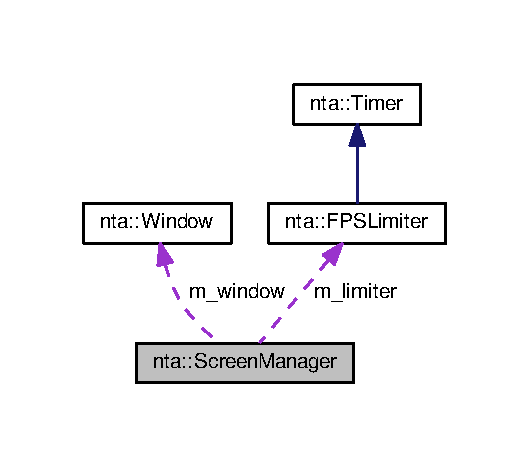
\includegraphics[width=350pt]{d6/d00/classnta_1_1ScreenManager__coll__graph}
\end{center}
\end{figure}


\subsection{Member Function Documentation}
\mbox{\Hypertarget{classnta_1_1ScreenManager_a4b26e8adc481bfb37a088e047e4ccc2a}\label{classnta_1_1ScreenManager_a4b26e8adc481bfb37a088e047e4ccc2a}} 
\index{nta\+::\+Screen\+Manager@{nta\+::\+Screen\+Manager}!get\+Curr\+Screen@{get\+Curr\+Screen}}
\index{get\+Curr\+Screen@{get\+Curr\+Screen}!nta\+::\+Screen\+Manager@{nta\+::\+Screen\+Manager}}
\subsubsection{\texorpdfstring{get\+Curr\+Screen()}{getCurrScreen()}}
{\footnotesize\ttfamily \hyperlink{classnta_1_1Screen}{Screen} $\ast$ nta\+::\+Screen\+Manager\+::get\+Curr\+Screen (\begin{DoxyParamCaption}{ }\end{DoxyParamCaption}) const}



returns the active screen 

\begin{DoxyRefDesc}{Todo}
\item[\hyperlink{todo__todo000009}{Todo}]write log error if m\+\_\+curr\+Screen is out of range \end{DoxyRefDesc}


Definition at line 14 of file Screen\+Manager.\+cpp.



Referenced by run(), and switch\+Screen().

Here is the caller graph for this function\+:
\nopagebreak
\begin{figure}[H]
\begin{center}
\leavevmode
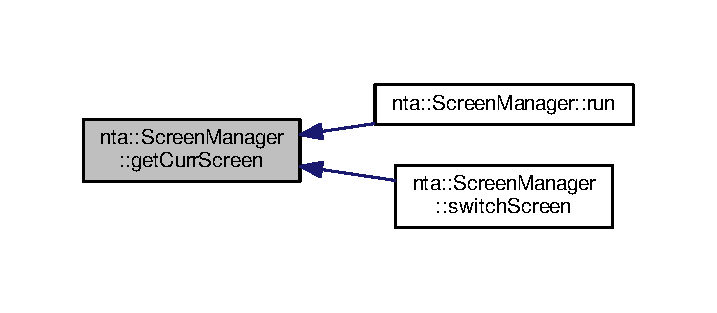
\includegraphics[width=344pt]{d0/dc4/classnta_1_1ScreenManager_a4b26e8adc481bfb37a088e047e4ccc2a_icgraph}
\end{center}
\end{figure}


The documentation for this class was generated from the following files\+:\begin{DoxyCompactItemize}
\item 
include/nta/Screen\+Manager.\+h\item 
src/Screen\+Manager.\+cpp\end{DoxyCompactItemize}

\hypertarget{structnta_1_1ScreenSwitchInfo}{}\section{nta\+:\+:Screen\+Switch\+Info Struct Reference}
\label{structnta_1_1ScreenSwitchInfo}\index{nta\+::\+Screen\+Switch\+Info@{nta\+::\+Screen\+Switch\+Info}}


Info passed to \hyperlink{classnta_1_1Screen_a895548cdf2a5170d671983fc9189579a}{Screen\+::on\+Focus}.  




{\ttfamily \#include $<$Screen.\+h$>$}

\subsection*{Public Member Functions}
\begin{DoxyCompactItemize}
\item 
\mbox{\Hypertarget{structnta_1_1ScreenSwitchInfo_a8d35bf79c11197bd91325798f5e4ed1c}\label{structnta_1_1ScreenSwitchInfo_a8d35bf79c11197bd91325798f5e4ed1c}} 
{\bfseries Screen\+Switch\+Info} (void $\ast$\hyperlink{structnta_1_1ScreenSwitchInfo_aed1a9c21a062863f6777c0cf3a00f23e}{data})
\item 
\mbox{\Hypertarget{structnta_1_1ScreenSwitchInfo_a6ad26e7cd2339ac667e1d1f909eacecb}\label{structnta_1_1ScreenSwitchInfo_a6ad26e7cd2339ac667e1d1f909eacecb}} 
{\bfseries Screen\+Switch\+Info} (void $\ast$\hyperlink{structnta_1_1ScreenSwitchInfo_aed1a9c21a062863f6777c0cf3a00f23e}{data}, int index)
\end{DoxyCompactItemize}
\subsection*{Public Attributes}
\begin{DoxyCompactItemize}
\item 
\mbox{\Hypertarget{structnta_1_1ScreenSwitchInfo_aed1a9c21a062863f6777c0cf3a00f23e}\label{structnta_1_1ScreenSwitchInfo_aed1a9c21a062863f6777c0cf3a00f23e}} 
void $\ast$ \hyperlink{structnta_1_1ScreenSwitchInfo_aed1a9c21a062863f6777c0cf3a00f23e}{data}
\begin{DoxyCompactList}\small\item\em arbitrary data to pass along \end{DoxyCompactList}\item 
\mbox{\Hypertarget{structnta_1_1ScreenSwitchInfo_a92f6d94b44a2945cbb0a6f93a98c9b94}\label{structnta_1_1ScreenSwitchInfo_a92f6d94b44a2945cbb0a6f93a98c9b94}} 
int \hyperlink{structnta_1_1ScreenSwitchInfo_a92f6d94b44a2945cbb0a6f93a98c9b94}{from\+Index}
\begin{DoxyCompactList}\small\item\em the index of the screen switched from \end{DoxyCompactList}\end{DoxyCompactItemize}


\subsection{Detailed Description}
Info passed to \hyperlink{classnta_1_1Screen_a895548cdf2a5170d671983fc9189579a}{Screen\+::on\+Focus}. 

Definition at line 31 of file Screen.\+h.



Collaboration diagram for nta\+:\+:Screen\+Switch\+Info\+:\nopagebreak
\begin{figure}[H]
\begin{center}
\leavevmode
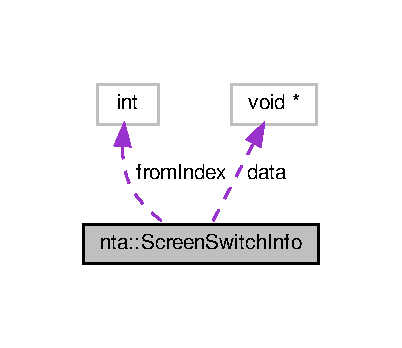
\includegraphics[width=193pt]{d3/d86/structnta_1_1ScreenSwitchInfo__coll__graph}
\end{center}
\end{figure}


The documentation for this struct was generated from the following file\+:\begin{DoxyCompactItemize}
\item 
include/nta/Screen.\+h\end{DoxyCompactItemize}

\hypertarget{classnta_1_1utils_1_1Semaphore}{}\section{nta\+:\+:utils\+:\+:Semaphore Class Reference}
\label{classnta_1_1utils_1_1Semaphore}\index{nta\+::utils\+::\+Semaphore@{nta\+::utils\+::\+Semaphore}}
\subsection*{Public Member Functions}
\begin{DoxyCompactItemize}
\item 
\mbox{\Hypertarget{classnta_1_1utils_1_1Semaphore_ae01dc768910e74be62cbc81765693f44}\label{classnta_1_1utils_1_1Semaphore_ae01dc768910e74be62cbc81765693f44}} 
\hyperlink{classnta_1_1utils_1_1Semaphore_ae01dc768910e74be62cbc81765693f44}{Semaphore} (int value=0)
\begin{DoxyCompactList}\small\item\em Constructs \hyperlink{classnta_1_1utils_1_1Semaphore}{Semaphore} with given value. \end{DoxyCompactList}\item 
\mbox{\Hypertarget{classnta_1_1utils_1_1Semaphore_a252683ad84d75e12d30f29441f7178bc}\label{classnta_1_1utils_1_1Semaphore_a252683ad84d75e12d30f29441f7178bc}} 
void \hyperlink{classnta_1_1utils_1_1Semaphore_a252683ad84d75e12d30f29441f7178bc}{wait} ()
\begin{DoxyCompactList}\small\item\em Halts until value of \hyperlink{classnta_1_1utils_1_1Semaphore}{Semaphore} is $>$ 0. \end{DoxyCompactList}\item 
\mbox{\Hypertarget{classnta_1_1utils_1_1Semaphore_ac80b0637a59c63cf9c553954c6cd0be9}\label{classnta_1_1utils_1_1Semaphore_ac80b0637a59c63cf9c553954c6cd0be9}} 
void \hyperlink{classnta_1_1utils_1_1Semaphore_ac80b0637a59c63cf9c553954c6cd0be9}{signal} ()
\begin{DoxyCompactList}\small\item\em Increments value of \hyperlink{classnta_1_1utils_1_1Semaphore}{Semaphore}. \end{DoxyCompactList}\item 
\mbox{\Hypertarget{classnta_1_1utils_1_1Semaphore_ad21972675a3dcc4c1876384ddd225fde}\label{classnta_1_1utils_1_1Semaphore_ad21972675a3dcc4c1876384ddd225fde}} 
{\bfseries Semaphore} (const \hyperlink{classnta_1_1utils_1_1Semaphore}{Semaphore} \&)=delete
\item 
\mbox{\Hypertarget{classnta_1_1utils_1_1Semaphore_afa2313271f3a4572f5dc8e79dff7a41f}\label{classnta_1_1utils_1_1Semaphore_afa2313271f3a4572f5dc8e79dff7a41f}} 
const \hyperlink{classnta_1_1utils_1_1Semaphore}{Semaphore} \& {\bfseries operator=} (const \hyperlink{classnta_1_1utils_1_1Semaphore}{Semaphore} \&)=delete
\end{DoxyCompactItemize}
\subsection*{Private Attributes}
\begin{DoxyCompactItemize}
\item 
\mbox{\Hypertarget{classnta_1_1utils_1_1Semaphore_a5d349e7ced70eb07eea6b9cfa50a6637}\label{classnta_1_1utils_1_1Semaphore_a5d349e7ced70eb07eea6b9cfa50a6637}} 
std\+::mutex \hyperlink{classnta_1_1utils_1_1Semaphore_a5d349e7ced70eb07eea6b9cfa50a6637}{m\+\_\+mutex}
\begin{DoxyCompactList}\small\item\em Thread safety stuff. \end{DoxyCompactList}\item 
\mbox{\Hypertarget{classnta_1_1utils_1_1Semaphore_a30bfcf40c58c71847933806aeab36b30}\label{classnta_1_1utils_1_1Semaphore_a30bfcf40c58c71847933806aeab36b30}} 
std\+::condition\+\_\+variable\+\_\+any {\bfseries m\+\_\+cv}
\item 
\mbox{\Hypertarget{classnta_1_1utils_1_1Semaphore_a7b21b47d4cfecfeeb97758916e23c9bc}\label{classnta_1_1utils_1_1Semaphore_a7b21b47d4cfecfeeb97758916e23c9bc}} 
int \hyperlink{classnta_1_1utils_1_1Semaphore_a7b21b47d4cfecfeeb97758916e23c9bc}{m\+\_\+value}
\begin{DoxyCompactList}\small\item\em The number of resources available. \end{DoxyCompactList}\end{DoxyCompactItemize}


\subsection{Detailed Description}


Definition at line 18 of file Thread\+Pool.\+h.



Collaboration diagram for nta\+:\+:utils\+:\+:Semaphore\+:
\nopagebreak
\begin{figure}[H]
\begin{center}
\leavevmode
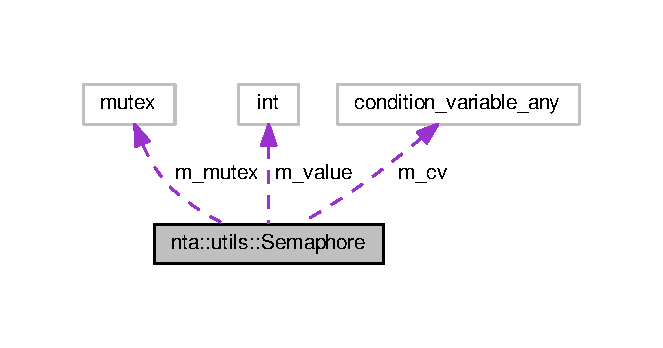
\includegraphics[width=318pt]{da/d79/classnta_1_1utils_1_1Semaphore__coll__graph}
\end{center}
\end{figure}


The documentation for this class was generated from the following files\+:\begin{DoxyCompactItemize}
\item 
include/nta/Thread\+Pool.\+h\item 
src/Semaphore.\+cpp\end{DoxyCompactItemize}

\hypertarget{classnta_1_1utils_1_1Json_1_1SetBeginEndKey}{}\section{nta\+:\+:utils\+:\+:Json\+:\+:Set\+Begin\+End\+Key Class Reference}
\label{classnta_1_1utils_1_1Json_1_1SetBeginEndKey}\index{nta\+::utils\+::\+Json\+::\+Set\+Begin\+End\+Key@{nta\+::utils\+::\+Json\+::\+Set\+Begin\+End\+Key}}


Key unlocking the set\+\_\+\{begin,end\}() \char`\"{}private\char`\"{} functions of class \hyperlink{classnta_1_1utils_1_1Json_1_1iterator}{Json\+::iterator}.  




{\ttfamily \#include $<$Json.\+h$>$}

\subsection*{Private Member Functions}
\begin{DoxyCompactItemize}
\item 
\mbox{\Hypertarget{classnta_1_1utils_1_1Json_1_1SetBeginEndKey_a8b763786a663ac1f4480536569502b03}\label{classnta_1_1utils_1_1Json_1_1SetBeginEndKey_a8b763786a663ac1f4480536569502b03}} 
{\bfseries Set\+Begin\+End\+Key} (const \hyperlink{classnta_1_1utils_1_1Json_1_1SetBeginEndKey}{Set\+Begin\+End\+Key} \&)
\item 
\mbox{\Hypertarget{classnta_1_1utils_1_1Json_1_1SetBeginEndKey_acedfb4474597563556da2ae4df424e5e}\label{classnta_1_1utils_1_1Json_1_1SetBeginEndKey_acedfb4474597563556da2ae4df424e5e}} 
\hyperlink{classnta_1_1utils_1_1Json_1_1SetBeginEndKey}{Set\+Begin\+End\+Key} \& {\bfseries operator=} (const \hyperlink{classnta_1_1utils_1_1Json_1_1SetBeginEndKey}{Set\+Begin\+End\+Key} \&)
\end{DoxyCompactItemize}
\subsection*{Friends}
\begin{DoxyCompactItemize}
\item 
\mbox{\Hypertarget{classnta_1_1utils_1_1Json_1_1SetBeginEndKey_a7dd8a79e9210a2a230d000eee63c6e8a}\label{classnta_1_1utils_1_1Json_1_1SetBeginEndKey_a7dd8a79e9210a2a230d000eee63c6e8a}} 
class {\bfseries Json}
\end{DoxyCompactItemize}


\subsection{Detailed Description}
Key unlocking the set\+\_\+\{begin,end\}() \char`\"{}private\char`\"{} functions of class \hyperlink{classnta_1_1utils_1_1Json_1_1iterator}{Json\+::iterator}. 

Definition at line 99 of file Json.\+h.



The documentation for this class was generated from the following file\+:\begin{DoxyCompactItemize}
\item 
include/nta/Json.\+h\end{DoxyCompactItemize}

\hypertarget{classnta_1_1SetIndicesKey}{}\section{nta\+:\+:Set\+Indices\+Key Class Reference}
\label{classnta_1_1SetIndicesKey}\index{nta\+::\+Set\+Indices\+Key@{nta\+::\+Set\+Indices\+Key}}


Key unlocking the set\+Indices() \char`\"{}private\char`\"{} function of class \hyperlink{classnta_1_1Screen}{Screen}.  




{\ttfamily \#include $<$Screen.\+h$>$}

\subsection*{Private Member Functions}
\begin{DoxyCompactItemize}
\item 
\mbox{\Hypertarget{classnta_1_1SetIndicesKey_a1b4bf4c2c1cedda8165b75fc9647943b}\label{classnta_1_1SetIndicesKey_a1b4bf4c2c1cedda8165b75fc9647943b}} 
{\bfseries Set\+Indices\+Key} (const \hyperlink{classnta_1_1SetIndicesKey}{Set\+Indices\+Key} \&)
\item 
\mbox{\Hypertarget{classnta_1_1SetIndicesKey_adef93d7ba4e08efef31699a128c1f6cc}\label{classnta_1_1SetIndicesKey_adef93d7ba4e08efef31699a128c1f6cc}} 
\hyperlink{classnta_1_1SetIndicesKey}{Set\+Indices\+Key} \& {\bfseries operator=} (const \hyperlink{classnta_1_1SetIndicesKey}{Set\+Indices\+Key} \&)
\end{DoxyCompactItemize}
\subsection*{Friends}
\begin{DoxyCompactItemize}
\item 
\mbox{\Hypertarget{classnta_1_1SetIndicesKey_a888edc649fed896d28811ec69f3f2066}\label{classnta_1_1SetIndicesKey_a888edc649fed896d28811ec69f3f2066}} 
class {\bfseries Screen\+Manager}
\end{DoxyCompactItemize}


\subsection{Detailed Description}
Key unlocking the set\+Indices() \char`\"{}private\char`\"{} function of class \hyperlink{classnta_1_1Screen}{Screen}. 

Definition at line 17 of file Screen.\+h.



The documentation for this class was generated from the following file\+:\begin{DoxyCompactItemize}
\item 
include/nta/Screen.\+h\end{DoxyCompactItemize}

\hypertarget{classnta_1_1SetManagerKey}{}\section{nta\+:\+:Set\+Manager\+Key Class Reference}
\label{classnta_1_1SetManagerKey}\index{nta\+::\+Set\+Manager\+Key@{nta\+::\+Set\+Manager\+Key}}


Key unlocking the set\+Manager() private function of class \hyperlink{classnta_1_1Screen}{Screen}.  




{\ttfamily \#include $<$Screen.\+h$>$}

\subsection*{Private Member Functions}
\begin{DoxyCompactItemize}
\item 
\mbox{\Hypertarget{classnta_1_1SetManagerKey_a39cf977d72e792fd57d861e46ff0de5a}\label{classnta_1_1SetManagerKey_a39cf977d72e792fd57d861e46ff0de5a}} 
{\bfseries Set\+Manager\+Key} (const \hyperlink{classnta_1_1SetManagerKey}{Set\+Manager\+Key} \&)
\item 
\mbox{\Hypertarget{classnta_1_1SetManagerKey_a2827a71fc493a6c61697c42dc999389e}\label{classnta_1_1SetManagerKey_a2827a71fc493a6c61697c42dc999389e}} 
\hyperlink{classnta_1_1SetManagerKey}{Set\+Manager\+Key} \& {\bfseries operator=} (const \hyperlink{classnta_1_1SetManagerKey}{Set\+Manager\+Key} \&)
\end{DoxyCompactItemize}
\subsection*{Friends}
\begin{DoxyCompactItemize}
\item 
\mbox{\Hypertarget{classnta_1_1SetManagerKey_a888edc649fed896d28811ec69f3f2066}\label{classnta_1_1SetManagerKey_a888edc649fed896d28811ec69f3f2066}} 
class {\bfseries Screen\+Manager}
\end{DoxyCompactItemize}


\subsection{Detailed Description}
Key unlocking the set\+Manager() private function of class \hyperlink{classnta_1_1Screen}{Screen}. 

Definition at line 10 of file Screen.\+h.



The documentation for this class was generated from the following file\+:\begin{DoxyCompactItemize}
\item 
include/nta/Screen.\+h\end{DoxyCompactItemize}

\hypertarget{classnta_1_1SetWindowKey}{}\section{nta\+:\+:Set\+Window\+Key Class Reference}
\label{classnta_1_1SetWindowKey}\index{nta\+::\+Set\+Window\+Key@{nta\+::\+Set\+Window\+Key}}


Key unlocking the set\+Window() \char`\"{}private\char`\"{} function of class \hyperlink{classnta_1_1Screen}{Screen}.  




{\ttfamily \#include $<$Screen.\+h$>$}

\subsection*{Private Member Functions}
\begin{DoxyCompactItemize}
\item 
\mbox{\Hypertarget{classnta_1_1SetWindowKey_a0f684f229f8eab0cb2344656dfb11a4f}\label{classnta_1_1SetWindowKey_a0f684f229f8eab0cb2344656dfb11a4f}} 
{\bfseries Set\+Window\+Key} (const \hyperlink{classnta_1_1SetWindowKey}{Set\+Window\+Key} \&)
\item 
\mbox{\Hypertarget{classnta_1_1SetWindowKey_abb91da101149ee2639f043b51ebf9def}\label{classnta_1_1SetWindowKey_abb91da101149ee2639f043b51ebf9def}} 
\hyperlink{classnta_1_1SetWindowKey}{Set\+Window\+Key} \& {\bfseries operator=} (const \hyperlink{classnta_1_1SetWindowKey}{Set\+Window\+Key} \&)
\end{DoxyCompactItemize}
\subsection*{Friends}
\begin{DoxyCompactItemize}
\item 
\mbox{\Hypertarget{classnta_1_1SetWindowKey_a888edc649fed896d28811ec69f3f2066}\label{classnta_1_1SetWindowKey_a888edc649fed896d28811ec69f3f2066}} 
class {\bfseries Screen\+Manager}
\end{DoxyCompactItemize}


\subsection{Detailed Description}
Key unlocking the set\+Window() \char`\"{}private\char`\"{} function of class \hyperlink{classnta_1_1Screen}{Screen}. 

Definition at line 24 of file Screen.\+h.



The documentation for this class was generated from the following file\+:\begin{DoxyCompactItemize}
\item 
include/nta/Screen.\+h\end{DoxyCompactItemize}

\hypertarget{classnta_1_1SoundEffect}{}\section{nta\+:\+:Sound\+Effect Class Reference}
\label{classnta_1_1SoundEffect}\index{nta\+::\+Sound\+Effect@{nta\+::\+Sound\+Effect}}


Represents a sound effect or short audio clip.  




{\ttfamily \#include $<$Audio\+Manager.\+h$>$}

\subsection*{Public Member Functions}
\begin{DoxyCompactItemize}
\item 
\mbox{\Hypertarget{classnta_1_1SoundEffect_a2955a9f115c4e3690a9ef82eb05d498c}\label{classnta_1_1SoundEffect_a2955a9f115c4e3690a9ef82eb05d498c}} 
void \hyperlink{classnta_1_1SoundEffect_a2955a9f115c4e3690a9ef82eb05d498c}{play} (int num\+Loops=0) const
\begin{DoxyCompactList}\small\item\em plays the sound effect \end{DoxyCompactList}\end{DoxyCompactItemize}
\subsection*{Friends}
\begin{DoxyCompactItemize}
\item 
\mbox{\Hypertarget{classnta_1_1SoundEffect_a85edaa7e5c3ae68dabadd5373890591e}\label{classnta_1_1SoundEffect_a85edaa7e5c3ae68dabadd5373890591e}} 
class {\bfseries Audio\+Manager}
\end{DoxyCompactItemize}


\subsection{Detailed Description}
Represents a sound effect or short audio clip. 

Definition at line 12 of file Audio\+Manager.\+h.



The documentation for this class was generated from the following file\+:\begin{DoxyCompactItemize}
\item 
include/nta/Audio\+Manager.\+h\end{DoxyCompactItemize}

\hypertarget{classnta_1_1Sprite}{}\section{nta\+:\+:Sprite Class Reference}
\label{classnta_1_1Sprite}\index{nta\+::\+Sprite@{nta\+::\+Sprite}}


represents a textured quad  




{\ttfamily \#include $<$Sprite.\+h$>$}

\subsection*{Public Member Functions}
\begin{DoxyCompactItemize}
\item 
\mbox{\Hypertarget{classnta_1_1Sprite_a5d208eb1b82f0a60155887b5f4103dbc}\label{classnta_1_1Sprite_a5d208eb1b82f0a60155887b5f4103dbc}} 
\hyperlink{classnta_1_1Sprite_a5d208eb1b82f0a60155887b5f4103dbc}{Sprite} ()
\begin{DoxyCompactList}\small\item\em constructor and destructor \end{DoxyCompactList}\item 
void \hyperlink{classnta_1_1Sprite_a1054dba693836caca9e755acc530d2fd}{init} (float x, float y, float w, float h, crstring image\+Path, float d=0)
\begin{DoxyCompactList}\small\item\em creates the sprite \end{DoxyCompactList}\item 
\mbox{\Hypertarget{classnta_1_1Sprite_a01e831cda46d73acd8a4eff3cb56d5d3}\label{classnta_1_1Sprite_a01e831cda46d73acd8a4eff3cb56d5d3}} 
void \hyperlink{classnta_1_1Sprite_a01e831cda46d73acd8a4eff3cb56d5d3}{render} () const
\begin{DoxyCompactList}\small\item\em renders the sprite \end{DoxyCompactList}\end{DoxyCompactItemize}


\subsection{Detailed Description}
represents a textured quad 

Definition at line 10 of file Sprite.\+h.



\subsection{Member Function Documentation}
\mbox{\Hypertarget{classnta_1_1Sprite_a1054dba693836caca9e755acc530d2fd}\label{classnta_1_1Sprite_a1054dba693836caca9e755acc530d2fd}} 
\index{nta\+::\+Sprite@{nta\+::\+Sprite}!init@{init}}
\index{init@{init}!nta\+::\+Sprite@{nta\+::\+Sprite}}
\subsubsection{\texorpdfstring{init()}{init()}}
{\footnotesize\ttfamily void nta\+::\+Sprite\+::init (\begin{DoxyParamCaption}\item[{float}]{x,  }\item[{float}]{y,  }\item[{float}]{w,  }\item[{float}]{h,  }\item[{crstring}]{image\+Path,  }\item[{float}]{d = {\ttfamily 0} }\end{DoxyParamCaption})}



creates the sprite 

first triangle

second triangle 

Definition at line 11 of file Sprite.\+cpp.



The documentation for this class was generated from the following files\+:\begin{DoxyCompactItemize}
\item 
include/nta/Sprite.\+h\item 
src/Sprite.\+cpp\end{DoxyCompactItemize}

\hypertarget{classnta_1_1SpriteBatch}{}\section{nta\+:\+:Sprite\+Batch Class Reference}
\label{classnta_1_1SpriteBatch}\index{nta\+::\+Sprite\+Batch@{nta\+::\+Sprite\+Batch}}


{\ttfamily \#include $<$Sprite\+Batch.\+h$>$}

\subsection*{Public Member Functions}
\begin{DoxyCompactItemize}
\item 
\mbox{\Hypertarget{classnta_1_1SpriteBatch_a554ec4ee678b6f97621d299e4a258f95}\label{classnta_1_1SpriteBatch_a554ec4ee678b6f97621d299e4a258f95}} 
\hyperlink{classnta_1_1SpriteBatch_a554ec4ee678b6f97621d299e4a258f95}{Sprite\+Batch} ()
\begin{DoxyCompactList}\small\item\em constructor and destructor \end{DoxyCompactList}\item 
\mbox{\Hypertarget{classnta_1_1SpriteBatch_a91cb54c5e459f9cb0142f7d4b6e3272c}\label{classnta_1_1SpriteBatch_a91cb54c5e459f9cb0142f7d4b6e3272c}} 
void \hyperlink{classnta_1_1SpriteBatch_a91cb54c5e459f9cb0142f7d4b6e3272c}{init} ()
\begin{DoxyCompactList}\small\item\em initializes the batch \end{DoxyCompactList}\item 
\mbox{\Hypertarget{classnta_1_1SpriteBatch_a8ceff37f4b281bfb1f627876bb420978}\label{classnta_1_1SpriteBatch_a8ceff37f4b281bfb1f627876bb420978}} 
void \hyperlink{classnta_1_1SpriteBatch_a8ceff37f4b281bfb1f627876bb420978}{begin} ()
\begin{DoxyCompactList}\small\item\em begins collection of glyphs for the batch \end{DoxyCompactList}\item 
\mbox{\Hypertarget{classnta_1_1SpriteBatch_abadacd5bfcfc6ed0cf5a4470a22010ed}\label{classnta_1_1SpriteBatch_abadacd5bfcfc6ed0cf5a4470a22010ed}} 
void \hyperlink{classnta_1_1SpriteBatch_abadacd5bfcfc6ed0cf5a4470a22010ed}{end} ()
\begin{DoxyCompactList}\small\item\em ends collection of glyphs and prepares to render \end{DoxyCompactList}\item 
\mbox{\Hypertarget{classnta_1_1SpriteBatch_aa703fb92d0bd42865c21fdfb2625660d}\label{classnta_1_1SpriteBatch_aa703fb92d0bd42865c21fdfb2625660d}} 
void \hyperlink{classnta_1_1SpriteBatch_aa703fb92d0bd42865c21fdfb2625660d}{add\+Glyph} (crvec4 pos\+Rect, crvec4 uv\+Rect, G\+Luint texture, float depth=N\+T\+A\+\_\+\+D\+E\+F\+A\+U\+L\+T\+\_\+\+D\+E\+P\+TH, crvec4 color=glm\+::vec4(1))
\begin{DoxyCompactList}\small\item\em adds a glyph to the batch \end{DoxyCompactList}\item 
\mbox{\Hypertarget{classnta_1_1SpriteBatch_a4a6041951ba065a9ad0e7265bef531ef}\label{classnta_1_1SpriteBatch_a4a6041951ba065a9ad0e7265bef531ef}} 
void {\bfseries add\+Glyph} (crvec2 corner1, crvec2 corner2, crvec4 uv\+Rect, G\+Luint texture, float depth=N\+T\+A\+\_\+\+D\+E\+F\+A\+U\+L\+T\+\_\+\+D\+E\+P\+TH, crvec4 color=glm\+::vec4(1))
\item 
\mbox{\Hypertarget{classnta_1_1SpriteBatch_a5bfd87da8549218f739977bb3fa3361c}\label{classnta_1_1SpriteBatch_a5bfd87da8549218f739977bb3fa3361c}} 
void {\bfseries add\+Glyph} (crvec4 pos\+Rect, crvec4 uv\+Rect, G\+Luint texture, crvec4 color, float depth=N\+T\+A\+\_\+\+D\+E\+F\+A\+U\+L\+T\+\_\+\+D\+E\+P\+TH)
\item 
\mbox{\Hypertarget{classnta_1_1SpriteBatch_a1acc97aec74cdd4709ea0e2bc064a3ce}\label{classnta_1_1SpriteBatch_a1acc97aec74cdd4709ea0e2bc064a3ce}} 
void {\bfseries add\+Glyph} (crvec2 corner1, crvec2 corner2, crvec4 uv\+Rect, G\+Luint texture, crvec4 color, float depth=N\+T\+A\+\_\+\+D\+E\+F\+A\+U\+L\+T\+\_\+\+D\+E\+P\+TH)
\item 
\mbox{\Hypertarget{classnta_1_1SpriteBatch_ae7566d38b0cdd33f2b3e16dfcf993714}\label{classnta_1_1SpriteBatch_ae7566d38b0cdd33f2b3e16dfcf993714}} 
void \hyperlink{classnta_1_1SpriteBatch_ae7566d38b0cdd33f2b3e16dfcf993714}{render} () const
\begin{DoxyCompactList}\small\item\em renders the batch \end{DoxyCompactList}\end{DoxyCompactItemize}
\subsection*{Private Member Functions}
\begin{DoxyCompactItemize}
\item 
\mbox{\Hypertarget{classnta_1_1SpriteBatch_a3355b0c2840d3d78c092508925bf9565}\label{classnta_1_1SpriteBatch_a3355b0c2840d3d78c092508925bf9565}} 
void \hyperlink{classnta_1_1SpriteBatch_a3355b0c2840d3d78c092508925bf9565}{create\+Vertex\+Array\+Object} ()
\begin{DoxyCompactList}\small\item\em creates the vertex array object \end{DoxyCompactList}\item 
\mbox{\Hypertarget{classnta_1_1SpriteBatch_af22e3c4af01fef017e9522021545928f}\label{classnta_1_1SpriteBatch_af22e3c4af01fef017e9522021545928f}} 
void \hyperlink{classnta_1_1SpriteBatch_af22e3c4af01fef017e9522021545928f}{create\+Render\+Batches} ()
\begin{DoxyCompactList}\small\item\em creates the render batches \end{DoxyCompactList}\item 
\mbox{\Hypertarget{classnta_1_1SpriteBatch_ae8cf94595c26211521df9e1580776289}\label{classnta_1_1SpriteBatch_ae8cf94595c26211521df9e1580776289}} 
void \hyperlink{classnta_1_1SpriteBatch_ae8cf94595c26211521df9e1580776289}{sort\+Glyphs} ()
\begin{DoxyCompactList}\small\item\em sorts the glyphs \end{DoxyCompactList}\end{DoxyCompactItemize}
\subsection*{Static Private Member Functions}
\begin{DoxyCompactItemize}
\item 
\mbox{\Hypertarget{classnta_1_1SpriteBatch_acd5b622817c1bab5c60de488b089f0f9}\label{classnta_1_1SpriteBatch_acd5b622817c1bab5c60de488b089f0f9}} 
static bool \hyperlink{classnta_1_1SpriteBatch_acd5b622817c1bab5c60de488b089f0f9}{compare\+Texture} (\hyperlink{structnta_1_1Glyph}{Glyph} $\ast$lhs, \hyperlink{structnta_1_1Glyph}{Glyph} $\ast$rhs)
\begin{DoxyCompactList}\small\item\em comparers used to sort \end{DoxyCompactList}\item 
\mbox{\Hypertarget{classnta_1_1SpriteBatch_ae7aea3ca736e40b3a861048e883eabdc}\label{classnta_1_1SpriteBatch_ae7aea3ca736e40b3a861048e883eabdc}} 
static bool {\bfseries compare\+Depth} (\hyperlink{structnta_1_1Glyph}{Glyph} $\ast$lhs, \hyperlink{structnta_1_1Glyph}{Glyph} $\ast$rhs)
\end{DoxyCompactItemize}
\subsection*{Private Attributes}
\begin{DoxyCompactItemize}
\item 
\mbox{\Hypertarget{classnta_1_1SpriteBatch_ae6c42878b427eef6fcd07aad0a60c6aa}\label{classnta_1_1SpriteBatch_ae6c42878b427eef6fcd07aad0a60c6aa}} 
std\+::vector$<$ \hyperlink{structnta_1_1Glyph}{Glyph} $\ast$ $>$ \hyperlink{classnta_1_1SpriteBatch_ae6c42878b427eef6fcd07aad0a60c6aa}{m\+\_\+glyph\+Pointers}
\begin{DoxyCompactList}\small\item\em pointers to the glyphs to be rendered (used for sorting) \end{DoxyCompactList}\item 
\mbox{\Hypertarget{classnta_1_1SpriteBatch_ac8291bea20d3a963bbe006587f35bf6f}\label{classnta_1_1SpriteBatch_ac8291bea20d3a963bbe006587f35bf6f}} 
std\+::vector$<$ \hyperlink{structnta_1_1Glyph}{Glyph} $>$ \hyperlink{classnta_1_1SpriteBatch_ac8291bea20d3a963bbe006587f35bf6f}{m\+\_\+glyphs}
\begin{DoxyCompactList}\small\item\em the glyphs to be rendered (used for fast vector operations) \end{DoxyCompactList}\item 
\mbox{\Hypertarget{classnta_1_1SpriteBatch_ae194b160a5de1c3a45ccebc570acd4b5}\label{classnta_1_1SpriteBatch_ae194b160a5de1c3a45ccebc570acd4b5}} 
std\+::vector$<$ \hyperlink{structnta_1_1RenderBatch}{Render\+Batch} $>$ \hyperlink{classnta_1_1SpriteBatch_ae194b160a5de1c3a45ccebc570acd4b5}{m\+\_\+render\+Batches}
\begin{DoxyCompactList}\small\item\em the render batches used for rendering the glyphs \end{DoxyCompactList}\item 
\mbox{\Hypertarget{classnta_1_1SpriteBatch_ad0606266e8d335e3e10692f64ece5a77}\label{classnta_1_1SpriteBatch_ad0606266e8d335e3e10692f64ece5a77}} 
G\+Luint \hyperlink{classnta_1_1SpriteBatch_ad0606266e8d335e3e10692f64ece5a77}{m\+\_\+vao} = 0
\begin{DoxyCompactList}\small\item\em ids of the vertex buffer object and vertex array object used to render the glyphs \end{DoxyCompactList}\item 
\mbox{\Hypertarget{classnta_1_1SpriteBatch_a80916f3903da74581339d9295d454367}\label{classnta_1_1SpriteBatch_a80916f3903da74581339d9295d454367}} 
G\+Luint {\bfseries m\+\_\+vbo} = 0
\end{DoxyCompactItemize}


\subsection{Detailed Description}
represents a collection of sprites to be drawn If you want to draw something without a texture, use \hyperlink{classnta_1_1PrimitiveBatch}{Primitive\+Batch} instead 

Definition at line 59 of file Sprite\+Batch.\+h.



Collaboration diagram for nta\+:\+:Sprite\+Batch\+:\nopagebreak
\begin{figure}[H]
\begin{center}
\leavevmode
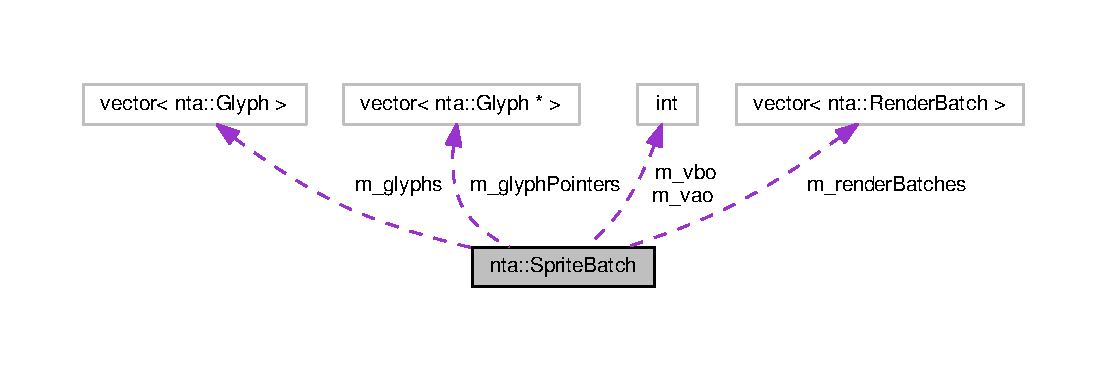
\includegraphics[width=350pt]{da/dc5/classnta_1_1SpriteBatch__coll__graph}
\end{center}
\end{figure}


The documentation for this class was generated from the following files\+:\begin{DoxyCompactItemize}
\item 
include/nta/Sprite\+Batch.\+h\item 
src/Sprite\+Batch.\+cpp\end{DoxyCompactItemize}

\hypertarget{classnta_1_1SpriteFont}{}\section{nta\+:\+:Sprite\+Font Class Reference}
\label{classnta_1_1SpriteFont}\index{nta\+::\+Sprite\+Font@{nta\+::\+Sprite\+Font}}


Loads in a .ttf file, creates a font texture from it, and is then used to render text.  




{\ttfamily \#include $<$Sprite\+Font.\+h$>$}

\subsection*{Public Member Functions}
\begin{DoxyCompactItemize}
\item 
\mbox{\Hypertarget{classnta_1_1SpriteFont_a195ee5502390cd373463a774641a4677}\label{classnta_1_1SpriteFont_a195ee5502390cd373463a774641a4677}} 
glm\+::vec2 \hyperlink{classnta_1_1SpriteFont_a195ee5502390cd373463a774641a4677}{measure} (crstring text) const
\begin{DoxyCompactList}\small\item\em returns the dimensions of the rectangle containing the text \end{DoxyCompactList}\item 
\mbox{\Hypertarget{classnta_1_1SpriteFont_afdd646f19b11d9c8128151afad994a77}\label{classnta_1_1SpriteFont_afdd646f19b11d9c8128151afad994a77}} 
void \hyperlink{classnta_1_1SpriteFont_afdd646f19b11d9c8128151afad994a77}{draw\+Text} (\hyperlink{classnta_1_1SpriteBatch}{Sprite\+Batch} \&batch, crstring text, crvec2 top\+Left, crvec2 scale, crvec4 color=glm\+::vec4(1), float depth=N\+T\+A\+\_\+\+D\+E\+F\+A\+U\+L\+T\+\_\+\+D\+E\+P\+TH) const
\begin{DoxyCompactList}\small\item\em renders text with specified location, color, scale, etc. \end{DoxyCompactList}\item 
\mbox{\Hypertarget{classnta_1_1SpriteFont_af2f85910e0f7fc8a2633088bf791da9f}\label{classnta_1_1SpriteFont_af2f85910e0f7fc8a2633088bf791da9f}} 
void {\bfseries draw\+Text} (\hyperlink{classnta_1_1SpriteBatch}{Sprite\+Batch} \&batch, crstring text, crvec4 pos\+Rect, crvec4 color=glm\+::vec4(1), float depth=N\+T\+A\+\_\+\+D\+E\+F\+A\+U\+L\+T\+\_\+\+D\+E\+P\+TH) const
\item 
\mbox{\Hypertarget{classnta_1_1SpriteFont_aafd62af3ce6a44354c07a372ba6db2fe}\label{classnta_1_1SpriteFont_aafd62af3ce6a44354c07a372ba6db2fe}} 
void {\bfseries draw\+Text} (\hyperlink{classnta_1_1SpriteBatch}{Sprite\+Batch} \&batch, crvec2 corner1, crvec2 corner2, crstring text, crvec4 color=glm\+::vec4(1), float depth=N\+T\+A\+\_\+\+D\+E\+F\+A\+U\+L\+T\+\_\+\+D\+E\+P\+TH) const
\item 
\mbox{\Hypertarget{classnta_1_1SpriteFont_ac5e60e0a7b6f9c0302c81f0d5b6628cc}\label{classnta_1_1SpriteFont_ac5e60e0a7b6f9c0302c81f0d5b6628cc}} 
void \hyperlink{classnta_1_1SpriteFont_ac5e60e0a7b6f9c0302c81f0d5b6628cc}{draw\+Texture} (\hyperlink{classnta_1_1SpriteBatch}{Sprite\+Batch} \&batch) const
\begin{DoxyCompactList}\small\item\em renders texture \end{DoxyCompactList}\end{DoxyCompactItemize}
\subsection*{Public Attributes}
\begin{DoxyCompactItemize}
\item 
\mbox{\Hypertarget{classnta_1_1SpriteFont_a1db301b9555c86340ea57bb2c5485dfc}\label{classnta_1_1SpriteFont_a1db301b9555c86340ea57bb2c5485dfc}} 
friend {\bfseries Resource\+Manager}
\end{DoxyCompactItemize}
\subsection*{Private Member Functions}
\begin{DoxyCompactItemize}
\item 
\hyperlink{classnta_1_1SpriteFont_a9dc96f31efd0830dcb476ea87534e358}{Sprite\+Font} (crstring font\+Path, unsigned int size)
\begin{DoxyCompactList}\small\item\em constructor -\/ creates a texture containing the font stored in font\+Path with glyphs of the given size \end{DoxyCompactList}\item 
\mbox{\Hypertarget{classnta_1_1SpriteFont_aa5292a1131ab6e04e23f282d2b067146}\label{classnta_1_1SpriteFont_aa5292a1131ab6e04e23f282d2b067146}} 
\hyperlink{classnta_1_1SpriteFont_aa5292a1131ab6e04e23f282d2b067146}{$\sim$\+Sprite\+Font} ()
\begin{DoxyCompactList}\small\item\em destructor \end{DoxyCompactList}\end{DoxyCompactItemize}
\subsection*{Private Attributes}
\begin{DoxyCompactItemize}
\item 
\mbox{\Hypertarget{classnta_1_1SpriteFont_a2fa17cff4bb7bd5125a01dcfa9b0fa88}\label{classnta_1_1SpriteFont_a2fa17cff4bb7bd5125a01dcfa9b0fa88}} 
\hyperlink{namespacenta_d4/d26/structnta_1_1CharGlyph}{Char\+Glyph} $\ast$ \hyperlink{classnta_1_1SpriteFont_a2fa17cff4bb7bd5125a01dcfa9b0fa88}{m\+\_\+char\+Glyphs} = nullptr
\begin{DoxyCompactList}\small\item\em a collection of glyphs for each char \end{DoxyCompactList}\item 
\mbox{\Hypertarget{classnta_1_1SpriteFont_ab74d460c526a4df82d206bba945fd711}\label{classnta_1_1SpriteFont_ab74d460c526a4df82d206bba945fd711}} 
G\+Luint \hyperlink{classnta_1_1SpriteFont_ab74d460c526a4df82d206bba945fd711}{m\+\_\+tex\+Id} = 0
\begin{DoxyCompactList}\small\item\em the idea of the generated texture \end{DoxyCompactList}\item 
\mbox{\Hypertarget{classnta_1_1SpriteFont_a689c80716d73871ea0d9abe08af9e8dc}\label{classnta_1_1SpriteFont_a689c80716d73871ea0d9abe08af9e8dc}} 
int \hyperlink{classnta_1_1SpriteFont_a689c80716d73871ea0d9abe08af9e8dc}{m\+\_\+font\+Height} = 0
\begin{DoxyCompactList}\small\item\em the height of the font \end{DoxyCompactList}\end{DoxyCompactItemize}


\subsection{Detailed Description}
Loads in a .ttf file, creates a font texture from it, and is then used to render text. 

Definition at line 52 of file Sprite\+Font.\+h.



Collaboration diagram for nta\+:\+:Sprite\+Font\+:
\nopagebreak
\begin{figure}[H]
\begin{center}
\leavevmode
\includegraphics[width=345pt]{da/dda/classnta_1_1SpriteFont__coll__graph}
\end{center}
\end{figure}


\subsection{Constructor \& Destructor Documentation}
\mbox{\Hypertarget{classnta_1_1SpriteFont_a9dc96f31efd0830dcb476ea87534e358}\label{classnta_1_1SpriteFont_a9dc96f31efd0830dcb476ea87534e358}} 
\index{nta\+::\+Sprite\+Font@{nta\+::\+Sprite\+Font}!Sprite\+Font@{Sprite\+Font}}
\index{Sprite\+Font@{Sprite\+Font}!nta\+::\+Sprite\+Font@{nta\+::\+Sprite\+Font}}
\subsubsection{\texorpdfstring{Sprite\+Font()}{SpriteFont()}}
{\footnotesize\ttfamily nta\+::\+Sprite\+Font\+::\+Sprite\+Font (\begin{DoxyParamCaption}\item[{crstring}]{font\+Path,  }\item[{unsigned int}]{size }\end{DoxyParamCaption})\hspace{0.3cm}{\ttfamily [private]}}



constructor -\/ creates a texture containing the font stored in font\+Path with glyphs of the given size 

\begin{DoxyRefDesc}{Todo}
\item[\hyperlink{todo__todo000003}{Todo}]Rename now that we\textquotesingle{}re no longer using simulated annealing \end{DoxyRefDesc}


Definition at line 7 of file Sprite\+Font.\+cpp.

Here is the call graph for this function\+:
\nopagebreak
\begin{figure}[H]
\begin{center}
\leavevmode
\includegraphics[width=350pt]{d6/d57/classnta_1_1SpriteFont_a9dc96f31efd0830dcb476ea87534e358_cgraph}
\end{center}
\end{figure}


The documentation for this class was generated from the following files\+:\begin{DoxyCompactItemize}
\item 
include/nta/Sprite\+Font.\+h\item 
src/Sprite\+Font.\+cpp\end{DoxyCompactItemize}

\hypertarget{structnta_1_1SpriteSheet}{}\section{nta\+:\+:Sprite\+Sheet Struct Reference}
\label{structnta_1_1SpriteSheet}\index{nta\+::\+Sprite\+Sheet@{nta\+::\+Sprite\+Sheet}}


Multiple sprites (each the same size) in one texture.  




{\ttfamily \#include $<$Animation2\+D.\+h$>$}

\subsection*{Public Member Functions}
\begin{DoxyCompactItemize}
\item 
\mbox{\Hypertarget{structnta_1_1SpriteSheet_acb0a6cab5e60d26a8e00d1e78974456b}\label{structnta_1_1SpriteSheet_acb0a6cab5e60d26a8e00d1e78974456b}} 
{\bfseries Sprite\+Sheet} (const \hyperlink{namespacenta_d3/dff/structnta_1_1GLTexture}{G\+L\+Texture} \&\hyperlink{structnta_1_1SpriteSheet_a6c55217abab2dbd76b61ad92fe902367}{tex}, crivec2 dims)
\item 
\mbox{\Hypertarget{structnta_1_1SpriteSheet_aca9119d89a8c2c9e8e88cc43844c264a}\label{structnta_1_1SpriteSheet_aca9119d89a8c2c9e8e88cc43844c264a}} 
{\bfseries Sprite\+Sheet} (crstring file\+\_\+path, crivec2 dims)
\item 
\mbox{\Hypertarget{structnta_1_1SpriteSheet_a68232c976caa805754f7b3863129ee09}\label{structnta_1_1SpriteSheet_a68232c976caa805754f7b3863129ee09}} 
{\bfseries Sprite\+Sheet} (crstring file\+\_\+path, int num\+\_\+cols)
\item 
glm\+::vec4 \hyperlink{structnta_1_1SpriteSheet_a618bc48e6978a19ad9eb56dda3307f5a}{get\+\_\+uv} (std\+::size\+\_\+t index) const
\item 
\mbox{\Hypertarget{structnta_1_1SpriteSheet_a98643a92390617ac5575b7a951e9805a}\label{structnta_1_1SpriteSheet_a98643a92390617ac5575b7a951e9805a}} 
glm\+::vec4 \hyperlink{structnta_1_1SpriteSheet_a98643a92390617ac5575b7a951e9805a}{get\+\_\+flipped\+\_\+uv} (std\+::size\+\_\+t index) const
\begin{DoxyCompactList}\small\item\em Like get\+\_\+uv except it flips the sprite horizontally. \end{DoxyCompactList}\end{DoxyCompactItemize}
\subsection*{Public Attributes}
\begin{DoxyCompactItemize}
\item 
\mbox{\Hypertarget{structnta_1_1SpriteSheet_a6c55217abab2dbd76b61ad92fe902367}\label{structnta_1_1SpriteSheet_a6c55217abab2dbd76b61ad92fe902367}} 
\hyperlink{namespacenta_d3/dff/structnta_1_1GLTexture}{G\+L\+Texture} \hyperlink{structnta_1_1SpriteSheet_a6c55217abab2dbd76b61ad92fe902367}{tex}
\begin{DoxyCompactList}\small\item\em The texture holding all the sprites. \end{DoxyCompactList}\item 
\mbox{\Hypertarget{structnta_1_1SpriteSheet_aad2a930c04420cdc26acbab618453d12}\label{structnta_1_1SpriteSheet_aad2a930c04420cdc26acbab618453d12}} 
\begin{tabbing}
xx\=xx\=xx\=xx\=xx\=xx\=xx\=xx\=xx\=\kill
union \{\\
\mbox{\Hypertarget{structnta_1_1SpriteSheet_a9cd7233cd82a28a0acbdbbec805e8a76}\label{structnta_1_1SpriteSheet_a9cd7233cd82a28a0acbdbbec805e8a76}} 
glm::ivec2 {\bfseries dims}\\
\mbox{\Hypertarget{structnta_1_1SpriteSheet_a0c707cf7e684dcea61a99b749fc90758}\label{structnta_1_1SpriteSheet_a0c707cf7e684dcea61a99b749fc90758}} 
\>struct \{\\
\mbox{\Hypertarget{structnta_1_1SpriteSheet_1_1_0D0_1_1_0D2_ac893c02f0affa345b63c86eb59f435b4}\label{structnta_1_1SpriteSheet_1_1_0D0_1_1_0D2_ac893c02f0affa345b63c86eb59f435b4}} 
int {\bfseries num\_rows}\\
\mbox{\Hypertarget{structnta_1_1SpriteSheet_1_1_0D0_1_1_0D2_a8f1bbf0a4ad76a8d7162354d9c19b41b}\label{structnta_1_1SpriteSheet_1_1_0D0_1_1_0D2_a8f1bbf0a4ad76a8d7162354d9c19b41b}} 
int {\bfseries num\_cols}\\
\>\} \\
\}; \\

\end{tabbing}\begin{DoxyCompactList}\small\item\em The dimensions of the sheat (rows x cols) \end{DoxyCompactList}\end{DoxyCompactItemize}


\subsection{Detailed Description}
Multiple sprites (each the same size) in one texture. 

Definition at line 8 of file Animation2\+D.\+h.



Collaboration diagram for nta\+:\+:Sprite\+Sheet\+:\nopagebreak
\begin{figure}[H]
\begin{center}
\leavevmode
\includegraphics[width=266pt]{d2/d89/structnta_1_1SpriteSheet__coll__graph}
\end{center}
\end{figure}


\subsection{Member Function Documentation}
\mbox{\Hypertarget{structnta_1_1SpriteSheet_a618bc48e6978a19ad9eb56dda3307f5a}\label{structnta_1_1SpriteSheet_a618bc48e6978a19ad9eb56dda3307f5a}} 
\index{nta\+::\+Sprite\+Sheet@{nta\+::\+Sprite\+Sheet}!get\+\_\+uv@{get\+\_\+uv}}
\index{get\+\_\+uv@{get\+\_\+uv}!nta\+::\+Sprite\+Sheet@{nta\+::\+Sprite\+Sheet}}
\subsubsection{\texorpdfstring{get\+\_\+uv()}{get\_uv()}}
{\footnotesize\ttfamily glm\+::vec4 nta\+::\+Sprite\+Sheet\+::get\+\_\+uv (\begin{DoxyParamCaption}\item[{std\+::size\+\_\+t}]{index }\end{DoxyParamCaption}) const\hspace{0.3cm}{\ttfamily [inline]}}

Gets U\+V-\/coordinates of specific sprite in the sheet

The topleft sprite is index 0 and indices increase moving to the right 

Definition at line 21 of file Animation2\+D.\+h.



Referenced by get\+\_\+flipped\+\_\+uv().

Here is the caller graph for this function\+:\nopagebreak
\begin{figure}[H]
\begin{center}
\leavevmode
\includegraphics[width=345pt]{d9/d85/structnta_1_1SpriteSheet_a618bc48e6978a19ad9eb56dda3307f5a_icgraph}
\end{center}
\end{figure}


The documentation for this struct was generated from the following files\+:\begin{DoxyCompactItemize}
\item 
include/nta/Animation2\+D.\+h\item 
src/Animation2\+D.\+cpp\end{DoxyCompactItemize}

\hypertarget{classnta_1_1SystemManager}{}\section{nta\+:\+:System\+Manager Class Reference}
\label{classnta_1_1SystemManager}\index{nta\+::\+System\+Manager@{nta\+::\+System\+Manager}}
\subsection*{Static Public Member Functions}
\begin{DoxyCompactItemize}
\item 
\mbox{\Hypertarget{classnta_1_1SystemManager_af37be3ff4538da0a95b5ca257187077c}\label{classnta_1_1SystemManager_af37be3ff4538da0a95b5ca257187077c}} 
static \hyperlink{classnta_1_1GLSLProgram}{G\+L\+S\+L\+Program} $\ast$ {\bfseries get\+G\+L\+S\+L\+Program} (crstring prog\+Path)
\item 
\mbox{\Hypertarget{classnta_1_1SystemManager_af3577fda5a1a1019f51fbc352047dc1f}\label{classnta_1_1SystemManager_af3577fda5a1a1019f51fbc352047dc1f}} 
static \hyperlink{classnta_1_1Window}{Window} $\ast$ {\bfseries get\+Window} (crstring window\+Title, int flags=0)
\item 
\mbox{\Hypertarget{classnta_1_1SystemManager_a69721eaa78fda16f0f028d2991672282}\label{classnta_1_1SystemManager_a69721eaa78fda16f0f028d2991672282}} 
static void {\bfseries destroy} ()
\end{DoxyCompactItemize}


\subsection{Detailed Description}


Definition at line 10 of file System\+Manager.\+h.



The documentation for this class was generated from the following files\+:\begin{DoxyCompactItemize}
\item 
include/nta/System\+Manager.\+h\item 
src/System\+Manager.\+cpp\end{DoxyCompactItemize}

\hypertarget{classnta_1_1utils_1_1ThreadPool}{}\section{nta\+:\+:utils\+:\+:Thread\+Pool Class Reference}
\label{classnta_1_1utils_1_1ThreadPool}\index{nta\+::utils\+::\+Thread\+Pool@{nta\+::utils\+::\+Thread\+Pool}}


Collection of threads for running scheduled functions.  




{\ttfamily \#include $<$Thread\+Pool.\+h$>$}

\subsection*{Classes}
\begin{DoxyCompactItemize}
\item 
struct \hyperlink{structnta_1_1utils_1_1ThreadPool_1_1worker}{worker}
\begin{DoxyCompactList}\small\item\em One thread available to the pool. \end{DoxyCompactList}\end{DoxyCompactItemize}
\subsection*{Public Member Functions}
\begin{DoxyCompactItemize}
\item 
\mbox{\Hypertarget{classnta_1_1utils_1_1ThreadPool_a3336e668eb283fcb65654058a9ed9113}\label{classnta_1_1utils_1_1ThreadPool_a3336e668eb283fcb65654058a9ed9113}} 
\hyperlink{classnta_1_1utils_1_1ThreadPool_a3336e668eb283fcb65654058a9ed9113}{Thread\+Pool} (size\+\_\+t num\+\_\+threads)
\begin{DoxyCompactList}\small\item\em Constructs a \hyperlink{classnta_1_1utils_1_1ThreadPool}{Thread\+Pool} with specified number of threads. \end{DoxyCompactList}\item 
\mbox{\Hypertarget{classnta_1_1utils_1_1ThreadPool_aa10c18b44db7449d04bb6577c70dc17b}\label{classnta_1_1utils_1_1ThreadPool_aa10c18b44db7449d04bb6577c70dc17b}} 
void \hyperlink{classnta_1_1utils_1_1ThreadPool_aa10c18b44db7449d04bb6577c70dc17b}{schedule} (const Thunk \&thunk)
\begin{DoxyCompactList}\small\item\em Schedules a function to be executed. \end{DoxyCompactList}\item 
\mbox{\Hypertarget{classnta_1_1utils_1_1ThreadPool_a267245d18bf040ebfb469cdce5221516}\label{classnta_1_1utils_1_1ThreadPool_a267245d18bf040ebfb469cdce5221516}} 
void \hyperlink{classnta_1_1utils_1_1ThreadPool_a267245d18bf040ebfb469cdce5221516}{wait} ()
\begin{DoxyCompactList}\small\item\em Waits for all scheduled functions to finish execution. \end{DoxyCompactList}\item 
\mbox{\Hypertarget{classnta_1_1utils_1_1ThreadPool_a3d928faed613a53dd61509dd8c10cf7a}\label{classnta_1_1utils_1_1ThreadPool_a3d928faed613a53dd61509dd8c10cf7a}} 
{\bfseries Thread\+Pool} (const \hyperlink{classnta_1_1utils_1_1ThreadPool}{Thread\+Pool} \&)=delete
\item 
\mbox{\Hypertarget{classnta_1_1utils_1_1ThreadPool_ac8f40f413b950d44672128dd9b51e5c7}\label{classnta_1_1utils_1_1ThreadPool_ac8f40f413b950d44672128dd9b51e5c7}} 
\hyperlink{classnta_1_1utils_1_1ThreadPool}{Thread\+Pool} \& {\bfseries operator=} (const \hyperlink{classnta_1_1utils_1_1ThreadPool}{Thread\+Pool} \&)=delete
\end{DoxyCompactItemize}
\subsection*{Private Member Functions}
\begin{DoxyCompactItemize}
\item 
void \hyperlink{classnta_1_1utils_1_1ThreadPool_a2ca98ba5ed4510e5aac90c0507859b8d}{dispatcher} ()
\begin{DoxyCompactList}\small\item\em Function run by dispatch thread. \end{DoxyCompactList}\item 
\mbox{\Hypertarget{classnta_1_1utils_1_1ThreadPool_ade9cec65b2ef535cb03fcc0ea941fe24}\label{classnta_1_1utils_1_1ThreadPool_ade9cec65b2ef535cb03fcc0ea941fe24}} 
void \hyperlink{classnta_1_1utils_1_1ThreadPool_ade9cec65b2ef535cb03fcc0ea941fe24}{worker\+\_\+func} (size\+\_\+t wid)
\begin{DoxyCompactList}\small\item\em Function run by worker threads. \end{DoxyCompactList}\item 
\mbox{\Hypertarget{classnta_1_1utils_1_1ThreadPool_a0cf734e83b83378a70a67864e9eeb732}\label{classnta_1_1utils_1_1ThreadPool_a0cf734e83b83378a70a67864e9eeb732}} 
size\+\_\+t \hyperlink{classnta_1_1utils_1_1ThreadPool_a0cf734e83b83378a70a67864e9eeb732}{get\+Available\+Worker} ()
\begin{DoxyCompactList}\small\item\em Returns id of an available worker. \end{DoxyCompactList}\item 
\mbox{\Hypertarget{classnta_1_1utils_1_1ThreadPool_a545314bb70fd5cd2ecbd8759d3251cc6}\label{classnta_1_1utils_1_1ThreadPool_a545314bb70fd5cd2ecbd8759d3251cc6}} 
bool \hyperlink{classnta_1_1utils_1_1ThreadPool_a545314bb70fd5cd2ecbd8759d3251cc6}{all\+Work\+Finished} ()
\begin{DoxyCompactList}\small\item\em Returns whether or not all work is finished. \end{DoxyCompactList}\end{DoxyCompactItemize}
\subsection*{Private Attributes}
\begin{DoxyCompactItemize}
\item 
\mbox{\Hypertarget{classnta_1_1utils_1_1ThreadPool_a7d4420324abe8ccd20040c9b66d2ae9e}\label{classnta_1_1utils_1_1ThreadPool_a7d4420324abe8ccd20040c9b66d2ae9e}} 
\begin{tabbing}
xx\=xx\=xx\=xx\=xx\=xx\=xx\=xx\=xx\=\kill
struct \{\\
\mbox{\Hypertarget{classnta_1_1utils_1_1ThreadPool_aea63e7307eb9e8202e4e7c7ee1ab0760}\label{classnta_1_1utils_1_1ThreadPool_aea63e7307eb9e8202e4e7c7ee1ab0760}} 
std::condition\_variable\_any {\bfseries cv}\\
\mbox{\Hypertarget{classnta_1_1utils_1_1ThreadPool_a04faf90c7795520116889f66d5b58b63}\label{classnta_1_1utils_1_1ThreadPool_a04faf90c7795520116889f66d5b58b63}} 
std::mutex {\bfseries m}\\
\} \hyperlink{classnta_1_1utils_1_1ThreadPool_a7d4420324abe8ccd20040c9b66d2ae9e}{m\_empty}\\

\end{tabbing}\begin{DoxyCompactList}\small\item\em Used to keep track of when the pool is empty. \end{DoxyCompactList}\item 
\mbox{\Hypertarget{classnta_1_1utils_1_1ThreadPool_a851ca4eb221b1d3961f345655bdabc7f}\label{classnta_1_1utils_1_1ThreadPool_a851ca4eb221b1d3961f345655bdabc7f}} 
std\+::vector$<$ \hyperlink{structnta_1_1utils_1_1ThreadPool_1_1worker}{worker} $>$ \hyperlink{classnta_1_1utils_1_1ThreadPool_a851ca4eb221b1d3961f345655bdabc7f}{m\+\_\+workers}
\begin{DoxyCompactList}\small\item\em The workers. \end{DoxyCompactList}\item 
\mbox{\Hypertarget{classnta_1_1utils_1_1ThreadPool_a36739b269f7de9e8676ec889ef0ec35b}\label{classnta_1_1utils_1_1ThreadPool_a36739b269f7de9e8676ec889ef0ec35b}} 
std\+::atomic$<$ bool $>$ \hyperlink{classnta_1_1utils_1_1ThreadPool_a36739b269f7de9e8676ec889ef0ec35b}{m\+\_\+kill}
\begin{DoxyCompactList}\small\item\em Sign to kill the pool. \end{DoxyCompactList}\item 
\mbox{\Hypertarget{classnta_1_1utils_1_1ThreadPool_a545160bd42d91789b0e91d33fe1a4c87}\label{classnta_1_1utils_1_1ThreadPool_a545160bd42d91789b0e91d33fe1a4c87}} 
\hyperlink{classnta_1_1utils_1_1Semaphore}{Semaphore} \hyperlink{classnta_1_1utils_1_1ThreadPool_a545160bd42d91789b0e91d33fe1a4c87}{m\+\_\+scheduled}
\begin{DoxyCompactList}\small\item\em Record of scheduled workers. \end{DoxyCompactList}\item 
\mbox{\Hypertarget{classnta_1_1utils_1_1ThreadPool_a2ae729ca0283f78900540a0109f418b5}\label{classnta_1_1utils_1_1ThreadPool_a2ae729ca0283f78900540a0109f418b5}} 
\hyperlink{classnta_1_1utils_1_1Semaphore}{Semaphore} \hyperlink{classnta_1_1utils_1_1ThreadPool_a2ae729ca0283f78900540a0109f418b5}{m\+\_\+available}
\begin{DoxyCompactList}\small\item\em Record of available workers. \end{DoxyCompactList}\item 
\mbox{\Hypertarget{classnta_1_1utils_1_1ThreadPool_a828f1c41f02f5ecce36e72a2a3328eb3}\label{classnta_1_1utils_1_1ThreadPool_a828f1c41f02f5ecce36e72a2a3328eb3}} 
std\+::queue$<$ Thunk $>$ \hyperlink{classnta_1_1utils_1_1ThreadPool_a828f1c41f02f5ecce36e72a2a3328eb3}{m\+\_\+funcs}
\begin{DoxyCompactList}\small\item\em The functions to be executed. \end{DoxyCompactList}\item 
\mbox{\Hypertarget{classnta_1_1utils_1_1ThreadPool_a6fe6bfa4607803f5f3f9b64b47c0417a}\label{classnta_1_1utils_1_1ThreadPool_a6fe6bfa4607803f5f3f9b64b47c0417a}} 
std\+::thread \hyperlink{classnta_1_1utils_1_1ThreadPool_a6fe6bfa4607803f5f3f9b64b47c0417a}{m\+\_\+dispatch\+\_\+thread}
\begin{DoxyCompactList}\small\item\em The thread for managing the pool. \end{DoxyCompactList}\end{DoxyCompactItemize}


\subsection{Detailed Description}
Collection of threads for running scheduled functions. 

Definition at line 38 of file Thread\+Pool.\+h.



Collaboration diagram for nta\+:\+:utils\+:\+:Thread\+Pool\+:\nopagebreak
\begin{figure}[H]
\begin{center}
\leavevmode
\includegraphics[width=350pt]{d2/d5d/classnta_1_1utils_1_1ThreadPool__coll__graph}
\end{center}
\end{figure}


\subsection{Member Function Documentation}
\mbox{\Hypertarget{classnta_1_1utils_1_1ThreadPool_a2ca98ba5ed4510e5aac90c0507859b8d}\label{classnta_1_1utils_1_1ThreadPool_a2ca98ba5ed4510e5aac90c0507859b8d}} 
\index{nta\+::utils\+::\+Thread\+Pool@{nta\+::utils\+::\+Thread\+Pool}!dispatcher@{dispatcher}}
\index{dispatcher@{dispatcher}!nta\+::utils\+::\+Thread\+Pool@{nta\+::utils\+::\+Thread\+Pool}}
\subsubsection{\texorpdfstring{dispatcher()}{dispatcher()}}
{\footnotesize\ttfamily void nta\+::utils\+::\+Thread\+Pool\+::dispatcher (\begin{DoxyParamCaption}{ }\end{DoxyParamCaption})\hspace{0.3cm}{\ttfamily [private]}}



Function run by dispatch thread. 

\begin{DoxyRefDesc}{Todo}
\item[\hyperlink{todo__todo000011}{Todo}]Can I reorganize to replace with a while(!kill)? \end{DoxyRefDesc}


Definition at line 28 of file Thread\+Pool.\+cpp.



Referenced by Thread\+Pool().

Here is the call graph for this function\+:\nopagebreak
\begin{figure}[H]
\begin{center}
\leavevmode
\includegraphics[width=350pt]{df/d5b/classnta_1_1utils_1_1ThreadPool_a2ca98ba5ed4510e5aac90c0507859b8d_cgraph}
\end{center}
\end{figure}
Here is the caller graph for this function\+:\nopagebreak
\begin{figure}[H]
\begin{center}
\leavevmode
\includegraphics[width=336pt]{df/d5b/classnta_1_1utils_1_1ThreadPool_a2ca98ba5ed4510e5aac90c0507859b8d_icgraph}
\end{center}
\end{figure}


The documentation for this class was generated from the following files\+:\begin{DoxyCompactItemize}
\item 
include/nta/Thread\+Pool.\+h\item 
src/Thread\+Pool.\+cpp\end{DoxyCompactItemize}

\hypertarget{classnta_1_1Timer}{}\section{nta\+:\+:Timer Class Reference}
\label{classnta_1_1Timer}\index{nta\+::\+Timer@{nta\+::\+Timer}}


represents a timer  




{\ttfamily \#include $<$Timer.\+h$>$}

\subsection*{Public Member Functions}
\begin{DoxyCompactItemize}
\item 
\mbox{\Hypertarget{classnta_1_1Timer_ac92420dd62672b399f1b4adfd81a4007}\label{classnta_1_1Timer_ac92420dd62672b399f1b4adfd81a4007}} 
\hyperlink{classnta_1_1Timer_ac92420dd62672b399f1b4adfd81a4007}{Timer} ()
\begin{DoxyCompactList}\small\item\em constructor and destructor \end{DoxyCompactList}\item 
\mbox{\Hypertarget{classnta_1_1Timer_a4192089df7b162096d119a7d9438173f}\label{classnta_1_1Timer_a4192089df7b162096d119a7d9438173f}} 
virtual void \hyperlink{classnta_1_1Timer_a4192089df7b162096d119a7d9438173f}{begin} ()
\begin{DoxyCompactList}\small\item\em begins timer \end{DoxyCompactList}\item 
\mbox{\Hypertarget{classnta_1_1Timer_adb7a179f51224cca3e4c2f8f8bc20a19}\label{classnta_1_1Timer_adb7a179f51224cca3e4c2f8f8bc20a19}} 
virtual long double \hyperlink{classnta_1_1Timer_adb7a179f51224cca3e4c2f8f8bc20a19}{end} () const
\begin{DoxyCompactList}\small\item\em return time since beginning of timer in nanoseconds \end{DoxyCompactList}\end{DoxyCompactItemize}
\subsection*{Protected Attributes}
\begin{DoxyCompactItemize}
\item 
\mbox{\Hypertarget{classnta_1_1Timer_adcd68ad6538a3e36b2f783996796ce56}\label{classnta_1_1Timer_adcd68ad6538a3e36b2f783996796ce56}} 
std\+::chrono\+::time\+\_\+point$<$ std\+::chrono\+::high\+\_\+resolution\+\_\+clock, std\+::chrono\+::nanoseconds $>$ {\bfseries m\+\_\+start\+Point}
\end{DoxyCompactItemize}


\subsection{Detailed Description}
represents a timer 

Definition at line 8 of file Timer.\+h.



Inheritance diagram for nta\+:\+:Timer\+:
\nopagebreak
\begin{figure}[H]
\begin{center}
\leavevmode
\includegraphics[width=165pt]{d3/d1b/classnta_1_1Timer__inherit__graph}
\end{center}
\end{figure}


Collaboration diagram for nta\+:\+:Timer\+:
\nopagebreak
\begin{figure}[H]
\begin{center}
\leavevmode
\includegraphics[width=221pt]{d3/def/classnta_1_1Timer__coll__graph}
\end{center}
\end{figure}


The documentation for this class was generated from the following files\+:\begin{DoxyCompactItemize}
\item 
include/nta/Timer.\+h\item 
src/Timer.\+cpp\end{DoxyCompactItemize}

\hypertarget{structnta_1_1Vertex2D}{}\section{nta\+:\+:Vertex2D Struct Reference}
\label{structnta_1_1Vertex2D}\index{nta\+::\+Vertex2D@{nta\+::\+Vertex2D}}


represents a vertex in 2 dimensions  




{\ttfamily \#include $<$Vertex.\+h$>$}

\subsection*{Public Member Functions}
\begin{DoxyCompactItemize}
\item 
\mbox{\Hypertarget{structnta_1_1Vertex2D_a696744d55f56ae170684266eab073c0f}\label{structnta_1_1Vertex2D_a696744d55f56ae170684266eab073c0f}} 
\hyperlink{structnta_1_1Vertex2D_a696744d55f56ae170684266eab073c0f}{Vertex2D} ()
\begin{DoxyCompactList}\small\item\em Initializes an \char`\"{}empty\char`\"{} vertex. \end{DoxyCompactList}\item 
\mbox{\Hypertarget{structnta_1_1Vertex2D_ab0988223c10ad83057c4ade8891b4814}\label{structnta_1_1Vertex2D_ab0988223c10ad83057c4ade8891b4814}} 
\hyperlink{structnta_1_1Vertex2D_ab0988223c10ad83057c4ade8891b4814}{Vertex2D} (crvec2 p)
\begin{DoxyCompactList}\small\item\em Initializes a white, textureless vertex with given position. \end{DoxyCompactList}\item 
\mbox{\Hypertarget{structnta_1_1Vertex2D_aa2e8619f157a72c64d2438f49ec65554}\label{structnta_1_1Vertex2D_aa2e8619f157a72c64d2438f49ec65554}} 
\hyperlink{structnta_1_1Vertex2D_aa2e8619f157a72c64d2438f49ec65554}{Vertex2D} (crvec2 p, crvec4 c)
\begin{DoxyCompactList}\small\item\em Initializes textureless, colorful vertex. \end{DoxyCompactList}\item 
\mbox{\Hypertarget{structnta_1_1Vertex2D_a1c2fe391aeb3ca6d0b8eebfbce1b5862}\label{structnta_1_1Vertex2D_a1c2fe391aeb3ca6d0b8eebfbce1b5862}} 
\hyperlink{structnta_1_1Vertex2D_a1c2fe391aeb3ca6d0b8eebfbce1b5862}{Vertex2D} (crvec2 p, crvec4 c, crvec2 u, float t=1.\+0)
\begin{DoxyCompactList}\small\item\em Initializes a vertex with everything. \end{DoxyCompactList}\item 
\mbox{\Hypertarget{structnta_1_1Vertex2D_a7079a91fd386eb3e4425c965f2ce2592}\label{structnta_1_1Vertex2D_a7079a91fd386eb3e4425c965f2ce2592}} 
void \hyperlink{structnta_1_1Vertex2D_a7079a91fd386eb3e4425c965f2ce2592}{set\+Position} (float x, float y)
\begin{DoxyCompactList}\small\item\em sets the position of the vertex \end{DoxyCompactList}\item 
\mbox{\Hypertarget{structnta_1_1Vertex2D_a12483720589a9836dd4628b2c2bc480c}\label{structnta_1_1Vertex2D_a12483720589a9836dd4628b2c2bc480c}} 
void \hyperlink{structnta_1_1Vertex2D_a12483720589a9836dd4628b2c2bc480c}{set\+Color} (float r, float g, float b, float a)
\begin{DoxyCompactList}\small\item\em sets the color of the vertex \end{DoxyCompactList}\item 
\mbox{\Hypertarget{structnta_1_1Vertex2D_a353285f6dc33e239b6c1290f50db1a3a}\label{structnta_1_1Vertex2D_a353285f6dc33e239b6c1290f50db1a3a}} 
void {\bfseries set\+Color} (crvec3 c)
\item 
\mbox{\Hypertarget{structnta_1_1Vertex2D_adb7b7e6498200e6f11965b0ecadeaa97}\label{structnta_1_1Vertex2D_adb7b7e6498200e6f11965b0ecadeaa97}} 
void \hyperlink{structnta_1_1Vertex2D_adb7b7e6498200e6f11965b0ecadeaa97}{set\+UV} (float u, float v)
\begin{DoxyCompactList}\small\item\em sets the uv coordinates of the vertex \end{DoxyCompactList}\end{DoxyCompactItemize}
\subsection*{Public Attributes}
\begin{DoxyCompactItemize}
\item 
\mbox{\Hypertarget{structnta_1_1Vertex2D_a27a44e1ca52b5a5a13d37495e9376636}\label{structnta_1_1Vertex2D_a27a44e1ca52b5a5a13d37495e9376636}} 
glm\+::vec2 \hyperlink{structnta_1_1Vertex2D_a27a44e1ca52b5a5a13d37495e9376636}{pos}
\begin{DoxyCompactList}\small\item\em the vertex\textquotesingle{}s position, color, and uv coordinates, respectively \end{DoxyCompactList}\item 
\mbox{\Hypertarget{structnta_1_1Vertex2D_a05016aff7572c60a2cb688e67b2a4a31}\label{structnta_1_1Vertex2D_a05016aff7572c60a2cb688e67b2a4a31}} 
glm\+::vec4 {\bfseries color}
\item 
\mbox{\Hypertarget{structnta_1_1Vertex2D_a71707b6c29cae0e883e76042e27e84d5}\label{structnta_1_1Vertex2D_a71707b6c29cae0e883e76042e27e84d5}} 
glm\+::vec2 {\bfseries uv}
\item 
\mbox{\Hypertarget{structnta_1_1Vertex2D_ac1b1fb722a89abaee9cddfb59543af85}\label{structnta_1_1Vertex2D_ac1b1fb722a89abaee9cddfb59543af85}} 
float {\bfseries has\+Texture}
\end{DoxyCompactItemize}
\subsection*{Static Public Attributes}
\begin{DoxyCompactItemize}
\item 
static const \hyperlink{namespacenta_df/d9d/structnta_1_1VertexAttrib}{Vertex\+Attrib} {\bfseries attribs} \mbox{[}N\+U\+M\+\_\+\+V\+E\+R\+T\+E\+X\+\_\+\+A\+T\+T\+R\+I\+BS\mbox{]}
\end{DoxyCompactItemize}


\subsection{Detailed Description}
represents a vertex in 2 dimensions 

Definition at line 20 of file Vertex.\+h.



Collaboration diagram for nta\+:\+:Vertex2D\+:\nopagebreak
\begin{figure}[H]
\begin{center}
\leavevmode
\includegraphics[width=350pt]{df/deb/structnta_1_1Vertex2D__coll__graph}
\end{center}
\end{figure}


\subsection{Member Data Documentation}
\mbox{\Hypertarget{structnta_1_1Vertex2D_a6be835338c31e6ce40e1a2f5a3039560}\label{structnta_1_1Vertex2D_a6be835338c31e6ce40e1a2f5a3039560}} 
\index{nta\+::\+Vertex2D@{nta\+::\+Vertex2D}!attribs@{attribs}}
\index{attribs@{attribs}!nta\+::\+Vertex2D@{nta\+::\+Vertex2D}}
\subsubsection{\texorpdfstring{attribs}{attribs}}
{\footnotesize\ttfamily const \hyperlink{namespacenta_df/d9d/structnta_1_1VertexAttrib}{Vertex\+Attrib} nta\+::\+Vertex2\+D\+::attribs\hspace{0.3cm}{\ttfamily [static]}}

{\bfseries Initial value\+:}
\begin{DoxyCode}
= \{
        \{2, GL\_FLOAT, GL\_FALSE, (\textcolor{keywordtype}{void}*)offsetof(\hyperlink{structnta_1_1Vertex2D_a696744d55f56ae170684266eab073c0f}{Vertex2D}, \hyperlink{structnta_1_1Vertex2D_a27a44e1ca52b5a5a13d37495e9376636}{pos})\},
        \{4, GL\_FLOAT, GL\_TRUE,  (\textcolor{keywordtype}{void}*)offsetof(\hyperlink{structnta_1_1Vertex2D_a696744d55f56ae170684266eab073c0f}{Vertex2D}, color)\},
        \{2, GL\_FLOAT, GL\_FALSE, (\textcolor{keywordtype}{void}*)offsetof(\hyperlink{structnta_1_1Vertex2D_a696744d55f56ae170684266eab073c0f}{Vertex2D}, uv)\},
        \{1, GL\_FLOAT, GL\_FALSE, (\textcolor{keywordtype}{void}*)offsetof(\hyperlink{structnta_1_1Vertex2D_a696744d55f56ae170684266eab073c0f}{Vertex2D}, hasTexture)\}
    \}
\end{DoxyCode}


Definition at line 62 of file Vertex.\+h.



The documentation for this struct was generated from the following files\+:\begin{DoxyCompactItemize}
\item 
include/nta/Vertex.\+h\item 
src/Vertex.\+cpp\end{DoxyCompactItemize}

\hypertarget{classnta_1_1Window}{}\section{nta\+:\+:Window Class Reference}
\label{classnta_1_1Window}\index{nta\+::\+Window@{nta\+::\+Window}}


Represent a window.  




{\ttfamily \#include $<$Window.\+h$>$}

\subsection*{Public Member Functions}
\begin{DoxyCompactItemize}
\item 
\mbox{\Hypertarget{classnta_1_1Window_a28534e4bb354c4b38b1d97aed78fd010}\label{classnta_1_1Window_a28534e4bb354c4b38b1d97aed78fd010}} 
\hyperlink{classnta_1_1Window_a28534e4bb354c4b38b1d97aed78fd010}{Window} ()
\begin{DoxyCompactList}\small\item\em constructor and destructor \end{DoxyCompactList}\item 
\mbox{\Hypertarget{classnta_1_1Window_a916d03b7cf059118106a4098eab11175}\label{classnta_1_1Window_a916d03b7cf059118106a4098eab11175}} 
S\+D\+L\+\_\+\+Window $\ast$ \hyperlink{classnta_1_1Window_a916d03b7cf059118106a4098eab11175}{get\+S\+D\+L\+Window} (\hyperlink{classnta_1_1GetSDLWindowKey}{Get\+S\+D\+L\+Window\+Key} key) const
\begin{DoxyCompactList}\small\item\em returns the underlying window \end{DoxyCompactList}\item 
\mbox{\Hypertarget{classnta_1_1Window_a461977bc0033732836ec56615ca0aa83}\label{classnta_1_1Window_a461977bc0033732836ec56615ca0aa83}} 
glm\+::vec2 \hyperlink{classnta_1_1Window_a461977bc0033732836ec56615ca0aa83}{get\+Dimensions} () const
\begin{DoxyCompactList}\small\item\em returns the window\textquotesingle{}s dimensions \end{DoxyCompactList}\item 
\mbox{\Hypertarget{classnta_1_1Window_a91f2eeac996c2f863b92601f8bb459aa}\label{classnta_1_1Window_a91f2eeac996c2f863b92601f8bb459aa}} 
std\+::string \hyperlink{classnta_1_1Window_a91f2eeac996c2f863b92601f8bb459aa}{get\+Title} () const
\begin{DoxyCompactList}\small\item\em returns the window\textquotesingle{}s title \end{DoxyCompactList}\item 
\mbox{\Hypertarget{classnta_1_1Window_ac6cb1a31bb8c219e189ca5f88e25dd45}\label{classnta_1_1Window_ac6cb1a31bb8c219e189ca5f88e25dd45}} 
int \hyperlink{classnta_1_1Window_ac6cb1a31bb8c219e189ca5f88e25dd45}{get\+Width} () const
\begin{DoxyCompactList}\small\item\em returns the width of the window \end{DoxyCompactList}\item 
\mbox{\Hypertarget{classnta_1_1Window_a0daae9b6ad0a0ea834f90e86a9416f88}\label{classnta_1_1Window_a0daae9b6ad0a0ea834f90e86a9416f88}} 
int \hyperlink{classnta_1_1Window_a0daae9b6ad0a0ea834f90e86a9416f88}{get\+Height} () const
\begin{DoxyCompactList}\small\item\em returns the height of the window \end{DoxyCompactList}\item 
\mbox{\Hypertarget{classnta_1_1Window_a23b55b95d017fe35655ed1287869bdf1}\label{classnta_1_1Window_a23b55b95d017fe35655ed1287869bdf1}} 
void \hyperlink{classnta_1_1Window_a23b55b95d017fe35655ed1287869bdf1}{resize} (int width, int height)
\begin{DoxyCompactList}\small\item\em resizes the window \end{DoxyCompactList}\item 
\mbox{\Hypertarget{classnta_1_1Window_a3dd8aab88817189b409643d75e476597}\label{classnta_1_1Window_a3dd8aab88817189b409643d75e476597}} 
void \hyperlink{classnta_1_1Window_a3dd8aab88817189b409643d75e476597}{set\+Dimensions} (int width, int height)
\begin{DoxyCompactList}\small\item\em updates the window\textquotesingle{}s stored dimensions \end{DoxyCompactList}\item 
\mbox{\Hypertarget{classnta_1_1Window_a5fdc643079410c14855a260ace84478e}\label{classnta_1_1Window_a5fdc643079410c14855a260ace84478e}} 
void \hyperlink{classnta_1_1Window_a5fdc643079410c14855a260ace84478e}{swap\+Buffers} () const
\begin{DoxyCompactList}\small\item\em updates the screen \end{DoxyCompactList}\item 
void \hyperlink{classnta_1_1Window_aa144f6bb014aaad3c91c3f3e6ad56f9c}{screenshot} () const
\begin{DoxyCompactList}\small\item\em stores a screenshot \end{DoxyCompactList}\end{DoxyCompactItemize}
\subsection*{Private Member Functions}
\begin{DoxyCompactItemize}
\item 
\mbox{\Hypertarget{classnta_1_1Window_a564ca2324e54c94f9e0f19d66017c07a}\label{classnta_1_1Window_a564ca2324e54c94f9e0f19d66017c07a}} 
void \hyperlink{classnta_1_1Window_a564ca2324e54c94f9e0f19d66017c07a}{create\+Window} (crstring title, int width, int height, int flags=0)
\begin{DoxyCompactList}\small\item\em creates a window \end{DoxyCompactList}\end{DoxyCompactItemize}
\subsection*{Private Attributes}
\begin{DoxyCompactItemize}
\item 
\mbox{\Hypertarget{classnta_1_1Window_a1e216236a7fdee82775fadef72a972ae}\label{classnta_1_1Window_a1e216236a7fdee82775fadef72a972ae}} 
S\+D\+L\+\_\+\+Window $\ast$ \hyperlink{classnta_1_1Window_a1e216236a7fdee82775fadef72a972ae}{m\+\_\+window}
\begin{DoxyCompactList}\small\item\em the window \end{DoxyCompactList}\item 
\mbox{\Hypertarget{classnta_1_1Window_a9034f9c0d5054ffd61782e2722432c63}\label{classnta_1_1Window_a9034f9c0d5054ffd61782e2722432c63}} 
std\+::string \hyperlink{classnta_1_1Window_a9034f9c0d5054ffd61782e2722432c63}{m\+\_\+title}
\begin{DoxyCompactList}\small\item\em the title of the window \end{DoxyCompactList}\item 
\mbox{\Hypertarget{classnta_1_1Window_aafa280d9434d31442028729eb0b01689}\label{classnta_1_1Window_aafa280d9434d31442028729eb0b01689}} 
int \hyperlink{classnta_1_1Window_aafa280d9434d31442028729eb0b01689}{m\+\_\+width}
\begin{DoxyCompactList}\small\item\em the dimensions of the window \end{DoxyCompactList}\item 
\mbox{\Hypertarget{classnta_1_1Window_a3857aecdc891f739b24030f7e8423529}\label{classnta_1_1Window_a3857aecdc891f739b24030f7e8423529}} 
int {\bfseries m\+\_\+height}
\end{DoxyCompactItemize}
\subsection*{Friends}
\begin{DoxyCompactItemize}
\item 
\mbox{\Hypertarget{classnta_1_1Window_ab1ef2aa9992dd8ae85793e1a1f980e1e}\label{classnta_1_1Window_ab1ef2aa9992dd8ae85793e1a1f980e1e}} 
class {\bfseries System\+Manager}
\end{DoxyCompactItemize}


\subsection{Detailed Description}
Represent a window. 

Definition at line 26 of file Window.\+h.



Collaboration diagram for nta\+:\+:Window\+:\nopagebreak
\begin{figure}[H]
\begin{center}
\leavevmode
\includegraphics[width=279pt]{da/daa/classnta_1_1Window__coll__graph}
\end{center}
\end{figure}


\subsection{Member Function Documentation}
\mbox{\Hypertarget{classnta_1_1Window_aa144f6bb014aaad3c91c3f3e6ad56f9c}\label{classnta_1_1Window_aa144f6bb014aaad3c91c3f3e6ad56f9c}} 
\index{nta\+::\+Window@{nta\+::\+Window}!screenshot@{screenshot}}
\index{screenshot@{screenshot}!nta\+::\+Window@{nta\+::\+Window}}
\subsubsection{\texorpdfstring{screenshot()}{screenshot()}}
{\footnotesize\ttfamily void nta\+::\+Window\+::screenshot (\begin{DoxyParamCaption}{ }\end{DoxyParamCaption}) const}



stores a screenshot 

\begin{DoxyRefDesc}{Todo}
\item[\hyperlink{todo__todo000017}{Todo}]Get rid of this? \end{DoxyRefDesc}


Definition at line 100 of file Window.\+cpp.

Here is the call graph for this function\+:\nopagebreak
\begin{figure}[H]
\begin{center}
\leavevmode
\includegraphics[width=350pt]{d4/dfb/classnta_1_1Window_aa144f6bb014aaad3c91c3f3e6ad56f9c_cgraph}
\end{center}
\end{figure}


The documentation for this class was generated from the following files\+:\begin{DoxyCompactItemize}
\item 
include/nta/Window.\+h\item 
src/Window.\+cpp\end{DoxyCompactItemize}

\hypertarget{structnta_1_1utils_1_1ThreadPool_1_1worker}{}\section{nta\+:\+:utils\+:\+:Thread\+Pool\+:\+:worker Struct Reference}
\label{structnta_1_1utils_1_1ThreadPool_1_1worker}\index{nta\+::utils\+::\+Thread\+Pool\+::worker@{nta\+::utils\+::\+Thread\+Pool\+::worker}}


One thread available to the pool.  


\subsection*{Public Attributes}
\begin{DoxyCompactItemize}
\item 
\mbox{\Hypertarget{structnta_1_1utils_1_1ThreadPool_1_1worker_a73546e576652ef9cded578d20e1de393}\label{structnta_1_1utils_1_1ThreadPool_1_1worker_a73546e576652ef9cded578d20e1de393}} 
std\+::thread \hyperlink{structnta_1_1utils_1_1ThreadPool_1_1worker_a73546e576652ef9cded578d20e1de393}{t}
\begin{DoxyCompactList}\small\item\em The thread owned by the worker. \end{DoxyCompactList}\item 
\mbox{\Hypertarget{structnta_1_1utils_1_1ThreadPool_1_1worker_af4dfab6b1c3168a40b90f518991d7efe}\label{structnta_1_1utils_1_1ThreadPool_1_1worker_af4dfab6b1c3168a40b90f518991d7efe}} 
Thunk \hyperlink{structnta_1_1utils_1_1ThreadPool_1_1worker_af4dfab6b1c3168a40b90f518991d7efe}{thunk}
\begin{DoxyCompactList}\small\item\em The function the worker is currently scheduled to execute. \end{DoxyCompactList}\item 
\mbox{\Hypertarget{structnta_1_1utils_1_1ThreadPool_1_1worker_ac891290ce8ae269990cbbd7243cd1817}\label{structnta_1_1utils_1_1ThreadPool_1_1worker_ac891290ce8ae269990cbbd7243cd1817}} 
std\+::atomic$<$ bool $>$ \hyperlink{structnta_1_1utils_1_1ThreadPool_1_1worker_ac891290ce8ae269990cbbd7243cd1817}{free}
\begin{DoxyCompactList}\small\item\em Whether or not the worker is free to take on a new function. \end{DoxyCompactList}\item 
\mbox{\Hypertarget{structnta_1_1utils_1_1ThreadPool_1_1worker_a7b1599c310dcbf3ed04639aff66fe06f}\label{structnta_1_1utils_1_1ThreadPool_1_1worker_a7b1599c310dcbf3ed04639aff66fe06f}} 
\hyperlink{classnta_1_1utils_1_1Semaphore}{Semaphore} {\bfseries task}
\end{DoxyCompactItemize}


\subsection{Detailed Description}
One thread available to the pool. 

Definition at line 40 of file Thread\+Pool.\+h.



Collaboration diagram for nta\+:\+:utils\+:\+:Thread\+Pool\+:\+:worker\+:
\nopagebreak
\begin{figure}[H]
\begin{center}
\leavevmode
\includegraphics[width=350pt]{da/d21/structnta_1_1utils_1_1ThreadPool_1_1worker__coll__graph}
\end{center}
\end{figure}


The documentation for this struct was generated from the following file\+:\begin{DoxyCompactItemize}
\item 
include/nta/Thread\+Pool.\+h\end{DoxyCompactItemize}

%--- End generated contents ---

% Index
\backmatter
\newpage
\phantomsection
\clearemptydoublepage
\addcontentsline{toc}{chapter}{Index}
\printindex

\end{document}
